% file: Propulsion.tex
% Propulsion, in unconventional ``grande'' format; fitting a widescreen format
% 
% github        : ernestyalumni
% linkedin      : ernestyalumni 
% wordpress.com : ernestyalumni
%
% This code is open-source, governed by the Creative Common license.  Use of this code is governed by the Caltech Honor Code: ``No member of the Caltech community shall take unfair advantage of any other member of the Caltech community.'' 
% 

\documentclass[10pt]{amsart}
\pdfoutput=1
%\usepackage{mathtools,amssymb,lipsum,caption}
\usepackage{mathtools,amssymb,caption}
\usepackage{graphicx}
\usepackage{hyperref}
\usepackage[utf8]{inputenc}
\usepackage{listings}
\usepackage[table]{xcolor}
\usepackage{pdfpages}
%\usepackage[version=3]{mhchem}
\usepackage{mhchem}

\usepackage{tikz}
\usetikzlibrary{matrix,arrows}

\usepackage{multicol}

\hypersetup{colorlinks=true,citecolor=[rgb]{0,0.4,0}}

\oddsidemargin=15pt
\evensidemargin=5pt
\hoffset-45pt
\voffset-55pt
\topmargin=-4pt
\headsep=5pt
\textwidth=1120pt
\textheight=595pt
\paperwidth=1200pt
\paperheight=700pt
\footskip=40pt








\newtheorem{theorem}{Theorem}
\newtheorem{corollary}{Corollary}
%\newtheorem*{main}{Main Theorem}
\newtheorem{lemma}{Lemma}
\newtheorem{proposition}{Proposition}

\newtheorem{definition}{Definition}
\newtheorem{remark}{Remark}

\newenvironment{claim}[1]{\par\noindent\underline{Claim:}\space#1}{}
\newenvironment{claimproof}[1]{\par\noindent\underline{Proof:}\space#1}{\hfill $\blacksquare$}

%This defines a new command \questionhead which takes one argument and
%prints out Question #. with some space.
\newcommand{\questionhead}[1]
  {\bigskip\bigskip
   \noindent{\small\bf Question #1.}
   \bigskip}

\newcommand{\problemhead}[1]
  {
   \noindent{\small\bf Problem #1.}
   }

\newcommand{\exercisehead}[1]
  { \smallskip
   \noindent{\small\bf Exercise #1.}
  }

\newcommand{\solutionhead}[1]
  {
   \noindent{\small\bf Solution #1.}
   }


\title{Propulsion}
\author{Ernest Yeung \href{mailto:ernestyalumni@gmail.com}{ernestyalumni@gmail.com}}
\date{13 novembre 2015}
\keywords{Propulsion, Rocket Propulsion, Thermodynamics, Fluid Flow, Fluid Mechanics}
\begin{document}

\definecolor{darkgreen}{rgb}{0,0.4,0}
\lstset{language=Python,
 frame=bottomline,
 basicstyle=\scriptsize,
 identifierstyle=\color{blue},
 keywordstyle=\bfseries,
 commentstyle=\color{darkgreen},
 stringstyle=\color{red},
 }
%\lstlistoflistings

\maketitle



\begin{multicols*}{2}

\setcounter{tocdepth}{1}
\tableofcontents



\begin{abstract}
Everything about Propulsion, with a focus on rocket propulsion.  

I also look at (rocket) propulsion for engineers from a (theoretical and mathematical) physicists' point of view.  I would like to seek more cross-polination between physicists and mathematicians and engineers in thermodynamics and fluid mechanics.
\end{abstract}

% This is my attempt at drawing a converging-diverging rocket nozzle in LaTeX picture environment. I ``eyeballed'' the dimensions from looking at the SpaceX Merlin engine picture on Wikipedia (``Merlin engine''), because I couldn't find on google search converging-diverging rocket nozzle dimensions; please let me know if there are any published diagrams, dimensions, or how people specify the dimensions on a drawing or mesh (or CAD?) of a rocket nozzle. Area expansion ratio is about 36
\setlength{\unitlength}{1cm}
\begin{picture}(10,5.5)(-5,-2.75)
\linethickness{1pt}
\put(0,1.0){\line(1,0){1.5}}
\put(0,-1.0){\line(1,0){1.5}}
\qbezier(1.5,1.0)(2.1,0.7)(2.3,0.6)
\qbezier(1.5,-1.0)(2.1,-0.7)(2.3,-0.6)
\put(2.3,0.6){\line(1,0){.2}}
\put(2.3,-0.6){\line(1,0){.2}}
\qbezier(2.5,0.6)(4.5,1.4)(7.5,1.8)
\qbezier(2.5,-0.6)(4.5,-1.4)(7.5,-1.8)
\end{picture}


\part{Notes and Solutions for \emph{Rocket Propulsion Elements} by George Sutton and Oscar Biblarz}


\section{Definitions and Fundamentals}

Ch. 2 Definitions and Fundamentals of Biblarz and Sutton (2001) \cite{GSuttonOBiblarz2001} 

Biblarz and Sutton (2001) \cite{GSuttonOBiblarz2001} says that \\
Propulsion is achieved by applying a force to a vehicle; \\
This propulsive force is obtained by ejecting propellant at high velocity.

Let surface $S$ of the rocket (with remaining fuel), choosing the normal unit vector of $S$, $\mathbf{n} \equiv \mathbf{n}_S$ to face outward. \\
Let the force, per unit area, field on a vehicle (also another word for rocket, plus remaining fuel) $\mathbf{f} = \mathbf{f}(t,\mathbf{x}), \, \forall \, \mathbf{x} \in S$. 

From pp. 144 of Frankel (2011) \cite{TFrankel2011}, vector integrals \emph{make no sense} on general manifolds (how could we add 2 vectors located at different points?!). The moral is that we naturally integrate differential forms, not vectors (i.e. vector fields) (cf. pp. xxxviii of Frankel (2011) \cite{TFrankel2011}).

\[
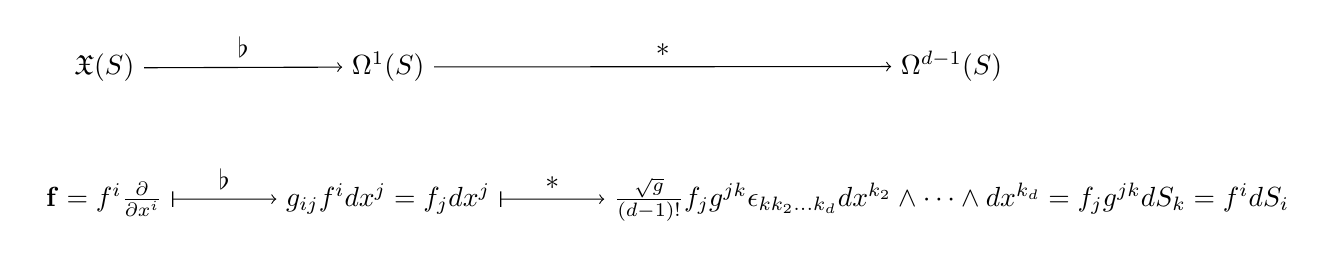
\begin{tikzpicture}
\matrix (m) [matrix of math nodes, row sep=2.8em, column sep=3.8em, minimum width=2.2em]
{
	\mathfrak{X}(S)         & \Omega^1(S) & \Omega^{d-1}(S)         \\
	\mathbf{f} = f^i \frac{\partial }{ \partial x^i}   &  g_{ij} f^i dx^j = f_j dx^j & \frac{\sqrt{g}}{ (d-1)!} f_j g^{jk} \epsilon_{k k_2 \dots k_d} dx^{k_2} \wedge \dots \wedge dx^{k_d} = f_j g^{jk} dS_k = f^i dS_i         \\
};
\path[->]
(m-1-1) edge node [auto] {$\flat$} (m-1-2)
(m-1-2) edge node [auto] {$*$} (m-1-3)
;
\path[|->]
(m-2-1) edge node [auto]  {$\flat$} (m-2-2)
(m-2-2) edge node [auto]  {$*$} (m-2-3)
;
\end{tikzpicture}
\]
for $dS_i := \frac{ \sqrt{g} }{ (d-1)! } \epsilon_{i i_2 \dots i_d } dx^{i_2} \wedge \dots \wedge dx^{i_d} \in \Omega^{d-1}(S)$, \\
and if $g_{ij} g^{jk} = \delta_i^{ \, \, k}$

Note that $f$ and $S$ are time-dependent in a fixed, inertial frame:
\[
\begin{aligned}
& \mathbf{f} = \mathbf{f}(t,\mathbf{x}) , \quad \, \forall \, \mathbf{x} \in S \\ 
& S = S(t)
\end{aligned}
\] 

Interpret 
\begin{equation}
\int_S * (\mathbf{f}(t, \mathbf{x}))^{\flat} \equiv F(t) \in \mathbf{R}
\end{equation}
as the net amount of force exerted on a rocket (with remaining fuel), by expelled propellants (at that instance, at the surface $S$).




\subsection{Definitions}

Section 2.1. ``Definitions'', Ch. 2 Definitions and Fundamentals of Biblarz and Sutton (2001) \cite{GSuttonOBiblarz2001} 

The \textbf{total impulse} $I_t$ is the thrust force $F_{\text{thrust}} = F_{\text{thrust}}(t)$ integrated over the burning time $T$, i.e. \\

total impulse $I_t = \int_0^T F_{\text{thrust}} dt $ \\
$t\equiv $ burning time $ \equiv t_p$ \\

specific impulse $I_s$, total impulse per unit weight of propellant

\[
I_s = \frac{ \int_0^t F_{\text{thrust}} dt }{ g_0 \int \dot{m} dt } = \frac{I_t}{ m_p g_0}
\]
\[
I_s = \frac{ \dot{m} u_e t_p }{ \dot{m} g t_p } = \frac{u_e}{g}
\]
If $F_{\text{thrust}} = \dot{m} u_e$, and constant propellant mass flow, $u_e$.

Instead, define 
\begin{definition}[total impulse]
\begin{equation}
\boxed{ I_{\text{tot}} \equiv I_t = \int_0^t dt F_{\text{thrust}}(t)	}
\end{equation}
\end{definition}

Let $m_{p, \text{exp}} = m_{p, \text{exp}}(t) = $ mass of propellant already expelled by time $t$. $m_{p, \text{exp}}(t) \in C^{\infty}(\mathbb{R})$.

Biblarz and Sutton (2001) \cite{GSuttonOBiblarz2001} defined \emph{specific impulse} to be the total impulse per unit weight of propellant as such:
\begin{definition}[Specific Impulse]
\begin{equation}
\boxed{ I_s := \frac{  \int_0^t dt F_{\text{thrust}}(t) }{ W_{p, \text{total expelled} }} }
\end{equation}
and so 
\begin{equation}
I_s = \frac{\int_0^t dt F_{\text{thrust}}(t) }{ g_0 \int dt \dot{m}_{p, \text{exp}}(t)}
\end{equation}
For practical calculations, 
\begin{equation}
I_s \frac{ \overline{F}_{\text{thrust} } }{ g_0 \overline{\dot{m}}_{p, \text{expelled}}  }
\end{equation}
\end{definition}
so it's more honest to say that it's the time-averaged specific impulse.

Note that $\int dt \dot{m}_{p, \text{exp}}(t) = m_{p, \text{exp}} = $ total effective propellant mass expelled through the nozzle.

If we are equipped with the exterior covariant derivative $D: \Omega^{d-1}(N; TN) \to \Omega^d(N; TN)$, then the force on a fluid over any general manifold is 
\[
F = \int_B \dot{m} \otimes \mathbf{u} + m \otimes \left( \frac{\partial \mathbf{u}}{ \partial t} + \nabla_{\mathbf{u}} \mathbf{u} \right) 
\]

If $\frac{\partial \mathbf{u}}{ \partial t} = 0$, $\nabla_{\mathbf{u}} \mathbf{u} = 0$ (no curved space),
\[
F = \int_B \dot{m} \otimes \mathbf{u}
\]
If $\mathbf{u}$ constant over $B$, call the \emph{effective exhaust velocity} $c \equiv u$ to be
\begin{equation}\label{Eq:ConstantEffectiveExhaustVelocity}
\begin{gathered}
F = \dot{m} u  \\
u = \frac{F}{\dot{m}} = I_s g_0
\end{gathered} 
\end{equation}
cf. Eq. 2-6 of Biblarz and Sutton (2001) \cite{GSuttonOBiblarz2001}

\textbf{Mass ratio} $\mathbf{MR}$ of a vehicle or \emph{particular vehicle stage} is defined as 
\[
\mathbf{MR} := \frac{m_f}{m_0}
\]
where, using Biblarz and Sutton (2001)'s notation, \\
$m_f \equiv $ final mass (after rocket operation has consumed all usable propellant), and \\
$m_0$ (before rocket operation).

$\mathbf{MR}$ applies to a single, or multistage vehicle.
\begin{itemize}
	\item Overall mass ratio is the product of the individual vehicle stage mass ratios
	\item Final mass $m_f$ is mass of vehicle after rocket has ceased to operate when all useful propellant mass $m_p$ has been consumed and ejected. 
	\item $m_f$ includes all components not useful propellant and may include guidance devices, navigation gear, \textbf{payload}
	\end{itemize} 

\subsubsection{Mass definitions for rockets, vehicles, propellants}

Instead, let the mass of the rocket $+$ remaining propellant be $M = M(t) \in C^{\infty}(\mathbb{R})$, such that $M \geq 0$, $\forall \, t \in \mathbb{R}$, always.

Let $M_f \in \mathbb{R}^+$ be a constant, what Biblarz and Sutton calls the final or inert propulsion mass, and denote as $m_f$.

Let $m_p = m_p(t) = $ propellant remaining on vehicle or stage. Thus,
\begin{equation}
\dot{m}_p \leq 0 
\end{equation}
which is expected by physical considerations.

Let 
\begin{equation}
m_p(t)  = m_p(0) - m_{p,\text{exp}}(t)
\end{equation}
where $m_{p,\text{exp}}(t) = $ total propellant that had been expelled. Clearly
\begin{equation}
\dot{m}_{p, \text{exp}}(t) > 0, \, m_{p,\text{exp}}(0) = 0
\end{equation}

Thus
\begin{equation}
\begin{aligned} 
& M(t) = M_f + m_p(t)  \\
& M(0) = M_f + m_p(0)
\end{aligned}
\end{equation}
and so define
\begin{definition}[Mass ratio]
\begin{equation}
\mathbf{MR} := \frac{M_f}{M(0)}	= \frac{M_f}{ M_f + m_p(0)}
\end{equation}
	\end{definition} 
and 
\begin{definition}[propellant mass fraction $\zeta$]
	\begin{equation}
	\zeta := \frac{m_p(0)}{ M(0)} = \frac{M(0) - M_f}{M(0)} = \frac{m_p(0)}{M_f + m_p(0)}
	\end{equation}
	\end{definition}
Biblarz and Sutton (2001) uses a different notation for the masses.

e.g. $\zeta = \frac{m_p(0)}{ M(0)} = 0.91$ means only 9 percent of mass is inert rocket hardware, and this small fraction contains, feeds, burns a substantially larger mass of propellant: a high value of $\zeta$ is desirable.

Impulse to weight ratio of a complete propulsion system:

\[
\frac{I_t}{w_0}
\]
$I_t \equiv $ total impulse, \\
$w_0 \equiv $ initial or propellant-loaded vehicle weight.

It's reasonable to suppose that 
\[
\begin{gathered}
\frac{I_t}{w_0} = \frac{I_t}{ M(0) g} = \frac{I_t}{  (M_f + m_p(0)) g_0} = \frac{I_s m_p(0) g_0}{ (M_f + m_p(0)) g_0} = \frac{ I_s}{ \frac{M_s}{m_p} + 1}
\end{gathered}
\]

thrust-to-weight ratio $F/w_0$





Example 2-1 of Biblarz and Sutton (2001) \cite{GSuttonOBiblarz2001} has some subtleties about the mass definitions that wasn't covered clearly (at least for me) by the discussion.

Let $M_r$ is the mass of the propulsion system, $r$ standing for "rocket." If there is \emph{no payload}, then 
\[
\begin{aligned} 
& M(0) = M_r + m_p(0) \\
& M(t) = M_r + m_p(t)
\end{aligned}
\]

\emph{But}, if payload is considered, observe that payload can be considered to be part of the whole of the vehicle (imagine an imaginary box surrounding the entire system or "vehicle"), \emph{and also} can be considered to be separate and distinct (no overlap) from the propulsion system plus propellant (imagine an imaginary box surrounding only the rocket (propulsion system) and fuel, and another imaginary box surrounding the payload; the two imaginary boxes do not overlap).

\[
\begin{aligned}
& M(0) = M_r + M_{\text{pay}} + m_p(0) \\
& M(t) = M_r + M_{\text{pay}} + m_p(t) 
\end{aligned}
\]

Recall that mass ratio is defined as $\mathbf{MR} := \frac{M_f}{ M(0)}$. But remember that $\mathbf{MR}$ can be considered for different, discrete imaginary boxes (subsystems). So for Example 2-1 of Biblarz and Sutton:

\[
\begin{aligned}
&	\mathbf{MR}_{\text{tot}} = \frac{M_{f, \text{tot}}}{M(0)} = \frac{M_r + M_{\text{pay}}}{ M(0) } \\
	& \mathbf{MR}_r = \frac{ M_r }{ M_r+ m_p(0)} = \frac{M_r }{ M(0) - M_{\text{pay}}}
\end{aligned}
\]
Notice how you can not take the payload mass into account; imagine only dealing with what's in the imaginary box surrounding only the rocket plus propellant.

If $\frac{\partial \mathbf{u}}{ \partial t} = 0$, assuming flat space, $F = \int_S \dot{m}_S \otimes \mathbf{u}$. Notice that for the units to make sense, $\dot{m}_S$ is the mass per unit (surface) area. If $\dot{m}_S , \mathbf{u}$ constant over surface area $S$, $F= \dot{m} \mathbf{u}$.  Then, $u = \frac{F}{\dot{m}} = I_s g_0$.

Then $\overline{u} = I_s g_0$.  
$I_{\text{tot}} = I_s m_p(0) = I_s(M(0) - (M_r + M_{\text{pay}}))$

Given the burn duration $T$, estimate $\dot{m}_{p, \text{exp}}$ with the simplest (linear) approximation:
$\dot{m}_{p, \text{exp}} = \frac{m_p(0)}{T}$.

$\overline{F}_{\text{thrust}} = \overline{ \dot{m}}_{p, \text{exp}} g_0 I_s$

Consider $\overline{F}_{\text{thrust}}$ on rocket, only. For a horizontal trajectory, max. acceleration is found at end of the thrusting schedule, just before shutdown (because while thrust is unchanged the mass is now at its minimum value). Think of "Max-Q".

\[
\Longrightarrow a_f = \frac{ \overline{F}_{\text{thrust}} }{ M_f}
\]
 
\subsection{Definitions with Thrust; effective exhaust velocity revisited}

Thrust is the force produced by a rocket propulsion system acting upon a vehicle.

In a simplified way, it's the reaction experienced by the structure due to ejection of matter at high velocity.

It represents the same phenomenon that pushes garden hose backwards or makes a gun recoil.  

In the latter case, forward momentum of the bullet and powder charge is equal to recoil or rearward momentum of gun barrel.

From pp. 30, Sec. 2.1. "Definitions" of Biblarz and Sutton (2001) \cite{GSuttonOBiblarz2001}, effective exhaust velocity $c$ was defined:
\begin{definition}[effective exhaust velocity]
effective exhaust velocity $c :=$ average equivalent velocity at which propellant is ejected from vehicle.
\end{definition}
Further, Biblarz and Sutton (2001) makes the assumption of uniform axial velocity $c$. But, in a rocket nozzle, the actual exhaust velocity is not uniform over the entire exit cross section, and doesn't represent the entire thrust magnitude. Nevertheless, Biblarz and Sutton (2001) gives the following formulas:
\[
c = I_s g_0 = F/\dot{m} 
\]
cf. Eq. 2-6 of Biblarz and Sutton (2001) \cite{GSuttonOBiblarz2001}.

Let's derive the thrust, due to the change in momentum.

\subsubsection{Momentum flux as a differential form}

Consider this object:
\[
u_x dx \wedge dy \wedge dz + u_y dy \wedge dz \wedge dx + u_z dz \wedge dx \wedge dy
\]

It is invariant under transformation $P$ such that $(x,y,z) \xrightarrow{P} (-x, -y, -z)$.

It is also invariant under $x \mapsto -x$ \textbf{and} $\mathbf{u} \mapsto -\mathbf{u}$, where $x$ could be $x, y$ or $z$.

Now
\[
\begin{gathered}
	u_x dx \wedge dy \wedge dz + u_y dy \wedge dz \wedge dx + u_z dz \wedge dx \wedge dy = \sum_{i=1}^3 \left( u_i dx^i \wedge \frac{\epsilon_{ijk}}{ 2!} dx^j \wedge dx^k \right) = \sum_{i=1}^3 \frac{u_i \epsilon_{ijk}}{ 2!} dx^i \wedge dx^j \wedge dx^k
\end{gathered}
\]

While the last expression is "manifestly covariant" in the indices $j$ and $k$ (i.e. the pair of "up" and "down" indices "match up"), it doesn't appear the case for the $i$ index. 



\subsubsection{Mass conservation}

Recall the derivation of mass conservation:

For time $t\in \mathbb{R}$ being a 1-dim. parameter, \\
given mass density $\rho = \rho(t,x) \in \mathbb{R} \times N$, $x\in N$, \\
volume form $\text{vol}^n\in \Omega^n(N)$ \\
on a smooth (spatial) manifold $N$, smooth submanifold with boundary $B(t) \subset N$, representing the control volume, \\
total mass inside a control volume $B(t)$, $m=m(t)$, is given by 
\[
m := \int_{B(t)} \rho \text{vol}^n
\]
Then for mass conservation,
\begin{equation}\label{Eq:MassConservationDerivation}
\begin{gathered}
\dot{m} \equiv \frac{d}{dt} m = \frac{d}{dt} \int_{B(t)} \rho \text{vol}^n = \int_{B(t)} \mathcal{L}_{\frac{\partial}{\partial t} + \mathbf{u}} (\rho \text{vol}^n) = \int_{B(t)} \left[ \frac{ \partial \rho }{ \partial t} \text{vol}^n + \mathcal{L}_{\mathbf{u}} (\rho \text{vol}^n) \right] = \int_{B(t)} \left[ \frac{ \partial \rho }{ \partial t} \text{vol}^n + \mathbf{d}(i_{\mathbf{u}} \rho \text{vol}^n) \right] = \\ 
 = \int_{B(t)} \frac{ \partial \rho }{ \partial t} \text{vol}^n + \int_{\partial B} i_{\mathbf{u}} \rho \text{vol}^n = \\
 = \int_{B(t)} \frac{ \partial \rho }{ \partial t} \text{vol}^n + \int_{\partial B}\rho u^i dS_i 
\end{gathered}
\end{equation}
where 
\[
\begin{gathered}
\mathcal{L}_{\mathbf{u}} (\rho \text{vol}^n ) = (\mathbf{d} i_{\mathbf{u}} + i_{\mathbf{u}} \mathbf{d}) (\rho \text{vol}^n) = \mathbf{d}(i_{\mathbf{u}} \rho \text{vol}^n) + 0 = \mathbf{d}i_{\mathbf{u}} \rho \text{vol}^n
\end{gathered} 
\]
is due to Cartan's magic formula, and 
\[
\int_{B(t)} \mathbf{d} (i_{\mathbf{u}} \rho \text{vol}^n) = \int_{\partial B(t)} i_{\mathbf{u}} \rho \text{vol}^n
\]
is by Stoke's law.


If $\frac{ \partial \rho }{ \partial t} = 0$ (steady-state condition), then
\[
\dot{m} = \int_{\partial B} \rho u^i dS_i
\]



\section{Nozzle Theory and Thermodynamic Relations}

\subsection{Isentropic Flow Through Nozzles}

Subsection 3.3 ``Isentropic Flow Through Nozzles'' of Biblarz and Sutton (2001) \cite{GSuttonOBiblarz2001} 

The Bernoulli invariant for compressible flow \footnote{\href{https://en.wikipedia.org/wiki/Euler_equations_\%28fluid_dynamics\%29\#Compressible_case}{``Euler equations (fluid dynamics)''}, Wikipedia} gives us this:
\[
\begin{gathered}
  h_1 + \frac{1}{2} v_1^2 = h_2 + \frac{1}{2} v_2^2 \text{ or } v_2 = \sqrt{ 2 (h_1 - h_2) + v_1^2 } \\
\Longrightarrow h_1 - h_2 = \frac{C_p}{MN}(\tau_1 - \tau_2) = \frac{ \gamma}{ \gamma -1} \frac{\tau_1}{M} \left( 1 - \frac{\tau_2}{\tau_1} \right) = \frac{ \gamma}{\gamma-1} \frac{\tau_1}{M} \left( 1 - \left( \frac{p_2}{p_1} \right)^{\frac{\gamma-1}{\gamma} } \right) = \frac{\gamma RT_1}{ \gamma -1} (1 - \left( \frac{p_2}{p_1} \right)^{\frac{\gamma-1}{\gamma } } )
\end{gathered}
\]
so that 
\[
v_2  = \sqrt{ \frac{2\gamma RT_1}{\gamma -1} \left(1- \left( \frac{p_2}{p_1} \right)^{\frac{\gamma-1}{\gamma} } \right) + v_1^2}
\]

When chamber section is large compared to nozzle throat section, chamber velocity or nozzle approach velocity comparatively small and $v_1^2$ can be neglected.\cite{GSuttonOBiblarz2001}

Chamber temperature $T_1$ at nozzle inlet; under isentropic conditions, $T_1$ differs little from stagnation temperature or (for chemical rocket) combustion temperature.\cite{GSuttonOBiblarz2001}

  

Ch. 4 Flight Performance of Biblarz and Sutton (2001) \cite{GSuttonOBiblarz2001} should probably be read before Ch. 3 Nozzle Theory and Thermodynamic Relations or before.  In AE121 Fall 2015, the material for Ch. 4 was covered in lectures (I think, from the problem sets) before Thermodynamics and Nozzle Theory.  

\cite{GSuttonOBiblarz2001}

\section{Flight Performance}

cf. Chapter 4 Flight Performance of Biblarz and Sutton (2001) \cite{GSuttonOBiblarz2001} 

\subsection{Gravity-Free, Drag-Free Space Flight}

Let \\
$m_p \equiv $ (total) propellant mass (initially) \\
$t_p \equiv$ propellant burning duration time  \\
Let mass of rocket $+$ propellant $M=M(t) = M(0) -m(t)$ s.t. $\begin{aligned} & \quad \\
  & m(0) = 0 \\
  & M(0) = M_0 +m_p \\
  & m(t_p) = m_p \\
  & M(t_p) = M_0 \end{aligned}$

If $\dot{m} = \frac{m_p}{t_p}$ (assume constant propellant flow rate),

\[
\begin{gathered}
  M=M(0) - \frac{m_p}{t_p}t = M(0)\left( 1 - \frac{m_p}{M(0)} \frac{t}{t_p} \right) = M(0) \left( 1 - \left( 1 - \frac{M(0) - m_p}{M(0) } \right) \frac{t}{t_p} \right)
\end{gathered}
\]
cf. Eq. 2-7 of Biblarz and Sutton (2001) \cite{GSuttonOBiblarz2001}.

Define some quantities:  mass ratio $= \frac{m_f}{m_0}$ where \\
$m_f := $ final mass (after rocket operation had consumed all usable propellant), which is $M_0$ above \\
$m_0 := $ mass before rocket operation, which is $M(0)$

propellant mass fraction $\frac{m_p}{M(0)}$ cf. Eq. 2-8 of Biblarz and Sutton (2001) \cite{GSuttonOBiblarz2001}.

For thrust $F_{\text{thrust}}$,
\[
\begin{gathered}
  F_{\text{thrust}} = \dot{m}u_e = M \frac{du}{dt} \Longrightarrow \frac{\dot{m}dt }{M} = \frac{du}{u_e} \text{ or } \frac{ \Delta u  }{u_e } = \int \frac{ \frac{m_p}{t_p} dt }{ M(0) - \frac{m_p}{t_p} t } = -\ln{ (M(0)- \frac{m_p}{t_p} t )} = \\
  = -\ln{ (M(0) - \frac{m_p}{t_p} t_p ) } + \ln{(M(0))} = \ln{ \left( \frac{M(0) }{M(0) - \frac{m_p}{t_p} t_p } \right) } = \ln{ \left( \frac{M(0)}{ M(0) - m_p } \right) }
\end{gathered}
\]
Thus
\[
\begin{gathered}
  \Delta u = u_e \ln{ \left( \frac{M(0)}{ M(0) - m_p } \right) } = u_e \ln{ \left( \frac{M(0)}{ M_0} \right) } \text{ or } \\
  \exp{ \left( \frac{ \Delta u }{ u_e } \right) }  = \frac{M(0)}{M(0) - m_p } = \frac{M(0)}{M_0} \text{ or } \frac{M_0}{M(0)} = \exp{ \left( \frac{ - \Delta u}{ u_e } \right) }
\end{gathered}
\]

Also remember that $F = \dot{m}u_e = \dot{m}I_{\text{sp}}g_0$, so $u_e \equiv $ effective exhaust velocity can be related directly to the specific impulse $I_{sp}$.  

Also note that for propellant mass fraction $\frac{m_p}{M(0)} < 1$, $\frac{m_p}{M(0)} = \frac{M(0) - M_0 }{M(0)} = 1 - \frac{M_0}{M(0)}$

\subsection{Forces Acting on a Vehicle in the Atmosphere}

assume starting and stopping transients very short and neglected, $F = u_e \dot{m}$

if mass rate of propellant consumption $\dot{m}$ constant, $\dot{m} = \frac{m_p}{t_p}$ so $F = \frac{m_p}{t_p} u_e$ 

drag $D$ \quad \, opposite to flight path due to resistance of body to motion in fluid \\
lift $L$ \quad \, normal to flight path 
\[
\begin{aligned}
  & L = C_L \frac{1}{2} \rho A u^2 \\ 
  & D = C_D \frac{1}{2} \rho A u^2 
\end{aligned}
\]
cf. Eqns. (4-10), (4-11) of Biblarz and Sutton (2001) \cite{GSuttonOBiblarz2001} 

density of earth's atmosphere can vary by factor up to 2 (for altitudes of 300 to 1200 km) \\
\phantom{\quad \, } depending on solar activity and night-to-day temperature variations. major unknown in drag

Assume neglect variation of gravity with geographical features and oblate shape of earth, 
\[
\begin{gathered}
  F = \frac{GM_e m}{r^2} \\
  mg_0 = \frac{GM_e}{R_0^2} m 
\end{gathered} \Longrightarrow \begin{gathered}
  g = g_0 \frac{R_0^2}{R^2} = g_0 \left( \frac{R_0}{R_0 + h } \right)^2
\end{gathered}
\]

\subsection{Basic Relations of Motion}

cf. Section 4.3 ``Basic Relations of Motion,'' Chapter 4 Flight Performance of Biblarz and Sutton (2001) \cite{GSuttonOBiblarz2001} 

\[
m \dot{\mathbf{u}} = \mathbf{F} - \mathbf{D} - m\mathbf{g}
\]
\[
\begin{gathered}
  \Longrightarrow \begin{aligned} & m \dot{u} = F\cos{(\psi - \theta) } - D - mg \sin{\theta}   \\
    & mu \frac{d\theta}{dt} = F\sin{(\psi - \theta) } + L - mg \cos{\theta} \end{aligned}
\end{gathered}
\]
$\psi = $ direction of thrust angle from horizontal reference

Consider perturbation effects (cf. Sec. 4.6, listed), drag and gravity

\[
\Longrightarrow \begin{aligned}
  & \dot{u} = \frac{F}{m} \cos{ (\psi - \theta) } - \frac{C_D}{2m} \rho Au^2 - g\sin{\theta} \\ 
  & u\dot{\theta} = \frac{F}{m} \sin{(\psi-\theta) } + \frac{C_L}{2m} \rho Au^2 - g\cos{\theta}
\end{aligned}
\]
$C_D,C_L$ are functions of velocity or Mach number (!!!)

For actual trajectory analyses, perturbation effects in Sec. 4.6 must be considered \\
\phantom{\quad \, } 3-body theory considered \\
\phantom{\quad \, } when propellant flow and thrust not constant 

from optical or radar tracking data, thrust or actual specific impulse during actual vehicle flights determined from accurately observed trajectory data. \\
\phantom{\quad \, } make assumption or measurement on propellant flow (which usually varies in a predetermined manner)

If $L=0$ (wingless rocket projectile), $\psi -\theta=0$ (flight direction $\theta$ same as thrust direction), and \\
$M(t) = M(0) - \dot{m}$; assume constant $\dot{m} = \frac{t}{t_p} m_p$ \\
$M(t) = M(0) - \frac{tm_p}{t_p} = M(0) ( 1 - \frac{m_p}{M(0)} \frac{t}{t_p} )$, with $\xi \equiv \frac{m_p}{M(0)}$ propellant mass ratio

\[
\begin{gathered}
  \dot{u} = \frac{F}{M} - \frac{C_D}{2M} \rho Au^2 - g\sin{\theta} = \frac{u_e \dot{m} }{ M} - \frac{C_D \rho Au^2}{2M} - g\sin{\theta} = \\
  = \frac{ u_e \xi \frac{t}{t_p} }{ 1 - \xi \frac{t}{t_p} }  - \frac{C_D \rho Au^2}{ 2M(0) ( 1 - \xi \frac{t}{t_p} ) } - g\sin{\theta}
\end{gathered}
\]
and 
\[
u\dot{\theta} = -g\cos{\theta}
\]

\textbf{Example 4-1}. Consider ``a simple-stage rocket for a rescue flare has the following characteristics and its flight path nomenclature is shown in the sketch.''

Neglect drag ``since flight velocities are low,'' assume no wind, assume local acceleration of gravity to be equal to sea level $g_0$, invariant throughout flight.  

\subsection*{Problems}

\problemhead{1} 
Recall that \[
\frac{M_0}{M(0)} = \exp{ \left( \frac{ - \Delta u}{ u_e } \right) }
\]
and so (in Python)
\begin{lstlisting}
import sympy
from sympy import *
>>> exp(-1600/2000.)
0.449328964117222
\end{lstlisting}

\problemhead{2} 
\[
\frac{m_p}{M(0)} = \frac{ M(0) - M_0 }{M(0)} = 1 - \frac{M_0}{M(0)} = 1 - \frac{1}{5} = 4/5 = 0.8
\]

\problemhead{3} dragless projectile, so $D=0$.  

\[
\dot{u} = -g_0 + \frac{ u_e }{ t_p( M(0)/m_p - t/t_p ) } \Longrightarrow \Delta u = -g_0 t -u_e \ln{ (1 - \frac{m_0 t}{M(0)t_p} ) }
\]
Plugging in $u_e = 2209 \, m/\text{sec}$, $m_p/M(0) = 0.57$, $t_p=5.0 \, \text{sec}$, $u_0=h_0=0$,

\verb|Propulsion.py|
\begin{lstlisting}
>>> integrate( flightpathdirection.subs(Drag,0).subs(psi,theta).subs(theta,pi/2).subs(F_thrust, m_p/t_p*u_e).
subs(M,M_constantflow).subs(m_p,M0*0.57).subs(t_p,5.).subs(u_e,2209.).subs(g_0,9.8).factor(M0).rhs, (t,0,5.0) )
1815.32988528061

Problem0403 = flightpathdirection.subs(Drag,0).subs(psi,theta).subs(theta,pi/2).subs(F_thrust, m_p/t_p*u_e).
subs(M,M_constantflow).subs(m_p,M0*0.57).subs(t_p,5.).subs(u_e,2209.).subs(g_0,9.8).factor(M0).rhs
\end{lstlisting}
\[
\boxed{ u_p = 1815 \, m/\text{sec}}
\]

\begin{lstlisting}
>>> integrate( integrate(Problem0403,(t,0,t) ),(t,0,5.0) )
3890.37850288891
\end{lstlisting}
\[
\boxed{ h_p = 3.89 \times 10^3 }
\]

\problemhead{4} How to estimate $A$ of the projectile?

\problemhead{5} 

Now
\[
\begin{gathered}
  M(t) a = F_{\text{thrust}} \\ 
  I_{sp} = \frac{ F_{\text{thrust}} t_p }{ g_0 \frac{m_p}{t_p }t_p } = \frac{ F_{\text{thrust}} t_p }{ g_0 m_p }
\end{gathered}
\]
and for $M(t) = M(0)- \frac{m_p}{t_p}t$, 
\[
\begin{gathered}
  a = \frac{ I_{sp} \left( \frac{g_0 m_p }{t_p} \right) }{ M(0) - \frac{m_p}{t_p} t } \leq a(t=t_p)
\end{gathered} \Longrightarrow a(t=t_p) = \frac{I_{sp} \left( \frac{g_0 m_p }{ t_p } \right) }{M_0 } = \frac{ I_{sp} g_0 }{t_p} \left( \frac{1}{ \frac{M(0)}{m_p} - 1 } \right)
\]
Plugging $a = 50 \, m/\text{sec}^2$ and solving for $t_p$, 
\begin{lstlisting}
>>> 260.*9.8/50.*(1/ ( 1/0.88 - 1 ) )
373.70666666666637
\end{lstlisting}
\begin{enumerate}
\item[(a)]
\[
\boxed{ 373.71 \, \text{sec} }
\]
maximum allowable burn time, assuming steady propellant mass flow
\item[(b)]
\[
a = \frac{I_{sp} g_0 \xi / t_p }{ 1 - \xi t/t_p } \Longrightarrow \Delta u = - I_{sp} g_0 \ln{ ( 1 - \xi t/t_p ) }
\]
so
\[
\Delta u = 5402.4 \, m/\text{sec}
\]
for maximum velocity relative to the launch vehicle
\end{enumerate}

\problemhead{6} Satellite in circular orbit
\[
\begin{gathered}
  F = \frac{GM_em}{(R_0+h)^2} = \frac{mv^2}{(R_0 + h) } \Longrightarrow \sqrt{ \frac{GM_0}{R_0 + h} } = v \\
  \frac{ 2 \pi (R_0 + h ) }{T} = v \Longrightarrow T = \frac{ 2\pi (R_0 +h)^{3/2} }{\sqrt{GM_e} } \\
  \frac{1}{2} mv^2 + \frac{-GM_e m }{ R_0 + h} - \left( \frac{ -GM_e m }{ R_0 } \right) = m \left[ \frac{1}{2} \frac{GM_e}{R_0 + h} - \frac{GM_e}{R_0 + h } + \frac{GM_e}{R_0} \right] = m \left[ GM_e \left( \frac{-1}{ 2(R_0 + h ) } + \frac{1}{R_0} \right) \right]
\end{gathered}
\]

Then run \verb|Propulsion.py| which now imports (\verb|import|) in Physique, a small package with the NIST (National Institute of Standards and Technology) Fundamental Constants \verb|FundConst|, NIST SI conversions \verb|conv|, and NASA Planetary Fact Sheet \verb|plnfacts| as Python \verb|pandas| DataFrames.  


\begin{lstlisting}
M_earth = plnfacts.loc[plnfacts['Planet']=="EARTH","Mass (1024kg)"].values[0]*10**(24) # in kg
R_earth = plnfacts.loc[plnfacts['Planet']=="EARTH","Diameter (km)"].values[0]/Decimal(2)

Gconst = FundConst[ FundConst["Quantity"].str.contains("gravitation") ].loc[243,"Value"]
v0406 = sqrt( Gconst*M_earth/((R_earth + Decimal(500))*10**3) )  
# velocity of satellite v of Chapter 4, Problem 6 of Biblarz and Sutton
7611.17633707692

T0406 = (2.*N(pi)*float((R_earth + Decimal(500))*10**3 )**(3./2))/float(sqrt( Gconst*M_earth)) 
# 5678 secs. or 1.58 hours

Eperm0406 = Gconst*M_earth*(-1/(2*((R_earth+Decimal(500))*10**3)) + 1/(R_earth*10**3)) 
# Energy per mass
'%.6E' % Eperm0406 # 33.51 MJ/kg
\end{lstlisting}  
\[
v = \boxed{ 7611 \, m/\text{sec} \, \quad \, T = 5678 \, s \text{ or } 1.58 \, \text{ hours }  \quad \, 33.51 \, MJ/kg }
\]

\part{Notes and Solutions for \emph{Space Propulsion Analysis and Design} by Humble, Henry, Larson}

cf. Humble, Henry, and Larson (1995) \cite{HHL1995}




\section{Thermodynamics of Fluid Flow; cf. Ch. 3. of Humble, Henry, and Larson (1995) \cite{HHL1995}}




cf. Humble, Henry, and Larson (1995), Ch. 3. Thermodynamics of Fluid Flow \cite{HHL1995} 


Chamber \\
Chamber conditions 
\[
(p_c, T_c, \rho_c) \in \mathbb{R}^2 \times \mathbb{R}_+
\]
$p_c = $ chamber pressure \\
$T_c = $ chamber temperature \\
$\rho_c = $ chamber density

Chamber characteristics \\
\begin{itemize} 
\item Combustion
\item high pressure $p_c$ 
\item high temperature $T_c$ 
\item very low net fluid velocity 
\end{itemize}

Nozzle. \\
exit conditions
$(p_e, T_e, \rho_e) \in \mathbb{R}^2 \times \mathbb{R}_+$ \\
$p_e = $ exit pressure \\
$T_e = $ exit temperature \\
$\rho_e = $ exit density 

Exit characteristics. 
\begin{itemize}
	\item flow expands to fill enlarged volume 
	\item reduced $p_e$ 
	\item reduced $T_e$
	\item very high fluid velocity 
\end{itemize}
Generalized View of a Rocket Thrust Chamber: \\
Understanding the thermodynamic conditions is key to understanding its performance

\subsection{3.1 Mass Transfer}

mass flow rate perpendicular to duct of cross-sectional area (A) is 
\[
\dot{m} = \rho v A
\]
$\dot{m} = $ mass flow rate (kg/s) \\
$\rho =$ fluid density (kg/$\text{m}^3$) \\
$v = $ fluid velocity ($m/s$) \\
$A = $ cross-sectional area of duct ($\text{m}^2$)

Control volume - region with constant shape and size that stays fixed in space \\
system approach (a.k.a. control mass approach) focus on fixed amount of matter \\
envelope containing the matter may change its size and shape, location \\
mass conservation (control-volume approach)

\[
\frac{d}{dt} (m_{cv}) = \dot{m}_{\text{in}} - \dot{m}_{\text{out}}
\]

$m_{cv} = $ amount of mass in control volume (kg) \\
$\dot{m}_{\text{in}} = $ mass flow rate into control volume (kg$/s$) \\
$\dot{m}_{\text{out}} = $ mass flow rate out of control volume (kg$/s$)

\[
\dot{m}= \int_{cs} \rho v dA
\]
$cs  = $ control surface \\
$\dot{m} = $ total mass flow through control surface (kg$/s$) \\
$\rho = $ fluid density in flow (kg$/m^3$) \\
$v = $ velocity of particles in flow (m$/s$)  \\
$dA = $ elemental area in control surface ($m^2$)



\subsection{3.2 Thermodynamic Relations (Energy and Entropy)}

cf. Humble, Henry, and Larson (1995), Ch. 3. Thermodynamics of Fluid Flow \cite{HHL1995}

\subsubsection{3.2.5. Isentropic Flow in One-Dimension}

cf. Humble, Henry, and Larson (1995), Ch. 3. Thermodynamics of Fluid Flow \cite{HHL1995}, pp. 95

\textbf{Simplifying Assumptions}

Fluid flow in a duct, applies to gaseous propellant in a nozzle, liquid or gaseous propellant in fuel plumbing, and coolant through nozzle's cooling tubes

\begin{enumerate}
\item isentropic flow, i.e. reversible and adiabatic; from the chamber (after combustion of propellant) to the nozzle exit. 
  \begin{itemize}
    \item \emph{adiabatic flow} means heat transfer doesn't dissipate energy from flow 
    \item   although heat transfer through chamber walls is significant, it's relatively small percentage of the total energy generated.
    \item This assumption also neglects effects of friction and fluid viscosity and doesn't apply to shock waves
  \end{itemize}
\item 1-dim. flow.\\

  larger nozzle cone half angle, less acceptable this assumption becomes.  For most nozzles, assumption causes less than 5% error.
\item products of combustion constitute a perfect gas
\item Frozen flow.  Once established in chamber, products of combustion don't change in hcemical composition while traversing nozzle
  \item steady flow
  \end{enumerate}

\emph{Isentropic Relations}  

energy conservation $\Longrightarrow Q = dU - W = dU + pdV$

reversible process $\Longrightarrow  Q = \tau d\sigma$ 

\[
\begin{aligned}
 &  \tau d\sigma = dU + pdV \\
  & dU = C_V d\tau \\
  & d\sigma = \frac{C_V}{\tau}d\tau + \frac{p}{\tau} dV = \frac{C_V}{\tau}d\tau + \frac{N}{V} dV 
\end{aligned}
\]

$d\sigma =0$ isentropic process
\[
\Longrightarrow 0 = \frac{C_V}{\tau}d\tau + \frac{N}{V} dV \text{ or } \frac{C_V}{\tau} d\tau = -\frac{N}{V} dV
  \]
  \[
\begin{gathered}
  \begin{aligned}  C_V \ln{ ( \tau_2 /\tau_1 ) } & = N \ln{ ( V_1 / V_2 ) } = \\
    & = (C_p - C_V) \ln{ (V_1/V_2) } \end{aligned} \\
  C_p = C_V + N \Longrightarrow \\
  \Longrightarrow \ln{ ( \tau_2/\tau_1) } = (\gamma -1) \ln{ (V_1/V_2) } \\
 \Longrightarrow \frac{\tau_2}{\tau_1} = \left( \frac{V_1}{V_2} \right)^{\gamma -1} = \left( \frac{\rho_2 }{\rho_1} \right)^{\gamma -1}
\end{gathered}
\]
with
\[
\begin{aligned}
  \gamma & \equiv \frac{C_p}{C_v} \\ 
  \gamma - 1 & = \frac{N}{C_V}
  \end{aligned}
\]

And so for \emph{isentropic, 1-dim., steady flow} and calorically perfect gas:

\begin{equation}
\begin{gathered}
  \begin{aligned}
    & (\tau_1, \rho_1) \mapsto (\tau_2, \rho_2) \\ 
    & (\tau_1, p_1) \mapsto (\tau_2, p_2) \\ 
    & (\rho_1, p_1) \mapsto (\rho_2, p_2) \\ 
  \end{aligned} \qquad \, \text{ with } \qquad \, \begin{aligned}
&    \frac{\tau_2}{\tau_1} = \left( \frac{\rho_2}{\rho_1} \right)^{\gamma-1} \text{ or } \frac{ \rho_1^{\gamma-1} }{ \tau_1} = \frac{ \rho_2^{\gamma-1}}{\tau_2} \\ 
 & \frac{p_2}{p_1} = \left( \frac{ \tau_2}{\tau_1} \right)^{ \frac{\gamma}{\gamma -1} } \\   
 & \frac{p_2}{p_1} = \left( \frac{ \rho_2}{\rho_1} \right)^{ \gamma } 
    \end{aligned}
\end{gathered}
  \end{equation}

From the Bernoulli invariant, and assuming
\begin{enumerate}
\item steady flow
\item adiabatic process (no heat transfer)
\item no significant changes in potential energy
  \item No shaft work or shear work done
\end{enumerate}
\begin{equation}
  h_1 + \frac{1}{2}u_1^2 = h_2 + \frac{1}{2}u_2^2
  \end{equation}
From
\[
\begin{gathered}
  \mathfrak{M} := \frac{u}{a} \\
a^2 = \frac{ \gamma \tau }{M} \\ 
 c_p \equiv \frac{ C_p}{MN}
\end{gathered} \text{ and } \begin{gathered}
  C_p = \frac{N}{\gamma -1} + N = N \left( \frac{\gamma}{\gamma -1} \right) \\
  \frac{C_p}{N} = \frac{\gamma }{ \gamma -1}  
\end{gathered} \Longrightarrow
\]
\[
\Longrightarrow 
\begin{gathered}
  c_p(\tau_1 - \tau_2) = \frac{1}{2} ( u_2^2 - u_1^2 ) = \\
  = \frac{1}{2} ( \mathfrak{M}_2^2 \gamma \tau_2 - \mathfrak{M}_1 \gamma \tau_1 ) \frac{1}{M} \\
  \Longrightarrow c_p \tau_1 + \frac{1}{2} \mathfrak{M}_1^2 \gamma \frac{\tau_1}{M} = ( c_p + \frac{1}{2} \mathfrak{M}_2^2 \frac{\gamma}{M } ) \tau_2 
  \end{gathered}
\]
\[
\begin{gathered}
  \Longrightarrow \frac{\tau_1}{\tau_2} = \frac{ \frac{C_p}{N} + \frac{1}{2} \mathfrak{M}_2^2 \gamma }{  \frac{C_p}{N} + \frac{1}{2} \mathfrak{M}_1^2 \gamma } = \frac{ \frac{\gamma}{\gamma -1} + \frac{1}{2} \mathfrak{M}_2^2 \gamma }{   \frac{\gamma}{\gamma -1} + \frac{1}{2} \mathfrak{M}_1^2 \gamma } = \frac{ 1 + \frac{1}{2} \mathfrak{M}_2^2 (\gamma -1 ) }{ 1 + \frac{1}{2} \mathfrak{M}_1^2 (\gamma -1 ) }
  \end{gathered}
\]

\textbf{Area ratio}

From Eq. \ref{Eq:AreastoMachs}, 
\begin{definition}[Expansion ratio]
  \begin{equation}
    \epsilon \equiv \text{ expansion ratio } := \frac{ A_{\text{exh}}}{ A_t} = \frac{1}{ \mathfrak{M}_{\text{exh}} } \left[ \left( 1 + \frac{\gamma -1}{2}  \mathfrak{M}_{\text{exh}}^2 \right) \frac{2}{ \gamma +1} \right]^{ \frac{\gamma +1}{ 2(\gamma -1) }}
    \end{equation}
  \end{definition}


So from
\[
\begin{gathered}
  \text{ mass conservation } \Longrightarrow  \dot{m} = \rho_t u_t A_T \\
  \text{ Mach number (definition) } \Longrightarrow \mathfrak{M}_t := u_t/a_t \\
  \frac{ \rho_t \tau_0}{M} = \frac{ \rho_0 \left( \frac{2}{\gamma +1} \right)^{\frac{1}{\gamma -1} } \tau_0 }{ M} = p_0 \left( \frac{2}{\gamma +1 } \right)^{ \frac{1}{\gamma -1} } \\
  \frac{1}{\gamma -1} + \frac{1}{2} = \frac{ 2 + \gamma - 1}{ \gamma -1} = \frac{ \gamma +1}{ \gamma -1} 
  \end{gathered}
\]

\[
\begin{gathered}
  \dot{m} u_{\text{exh}} = \rho_t \mathfrak{M}_t a_t A_t u_{\text{exh}} = \rho_t \left( \frac{\gamma \tau_t }{M} \right)^{1/2} A_t \left[ \frac{ 2\gamma }{\gamma -1} \frac{ \tau_0 }{M} \left( 1 - \left( \frac{p_e}{p_0} \right)^{\frac{\gamma -1}{\gamma } } \right) \right]^{1/2} = \frac{ \rho_t A_t }{M} \left[ \frac{ 2\gamma^2 \tau_t\tau_0 }{ \gamma -1} \left( 1 - \left( \frac{p_e}{p_0} \right)^{\frac{ \gamma -1}{\gamma } } \right) \right]^{1/2} = \\
  = p_0 \left( \frac{2}{\gamma + 1} \right)^{\frac{1}{\gamma -1 } } A_t \left[ \frac{2 \gamma^2}{ \gamma -1} \frac{ 2 }{ \gamma + 1} \left( 1 - \left( \frac{p_e}{p_0} \right)^{ \frac{\gamma -1}{\gamma } } \right) \right]^{1/2} = A_t p_0 \left[ \frac{ 2\gamma^2 }{ \gamma -1 } \left( \frac{2}{ \gamma + 1} \right)^{ \frac{ \gamma + 1}{ \gamma -1 } } \left( 1 - \left( \frac{p_e}{ p_0 } \right)^{ \frac{\gamma -1}{ \gamma } }\right) \right]^{1/2}
\end{gathered}
\]
So from
\[
F_{\text{thrust}} = \dot{m} u_{\text{exh}} + (p_e - p_a) A_e
\]
\begin{equation} \label{Eq:thrustidealrocket}
  \boxed{ 
  F_{\text{thrust}} = A_t p_0 \left[ \frac{ 2\gamma^2 }{ \gamma -1 } \left( \frac{2}{ \gamma + 1} \right)^{ \frac{ \gamma + 1}{ \gamma -1 } } \left( 1 - \left( \frac{p_e}{ p_0 } \right)^{ \frac{\gamma -1}{ \gamma } }\right) \right]^{1/2} + (p_e - p_a) A_{\text{exh}}  }
  \end{equation}

Eq. \ref{Eq:thrustidealrocket} is Eq. (3.129) of Humble, Henry, and Larson (1995), Ch. 3. Thermodynamics of Fluid Flow \cite{HHL1995}, pp. 112, Eq. (3-29) of Biblarz and Sutton (2001) \cite{GSuttonOBiblarz2001}, Ch. 3, pp. 63.  






\part{1-dim. propulsion (revisited)}

\section{Fluid Flow (review)}

\subsection{Mass conservation, revisited}

Let $m$ also denote the $d=3$ (differential) form, $m \in \Omega^d(N)$, where $N \equiv $ spatial manifold, $\text{dim}N = d =3$. Let $V$ be the control volume. Then
\[
\begin{gathered}
	M = \int_V m = \int_V \rho \text{vol}^d
\end{gathered}
\]

Recall then Eq. \ref{Eq:MassConservationDerivation}, so that 

\[
\begin{gathered}
\dot{M} \equiv \frac{d}{dt} M = \frac{d}{dt} \int_V \rho \text{vol}^d = \int_V \frac{ \partial \rho }{ \partial t} \text{vol}^d + \int_{\partial V} \rho u^i dS_i
\end{gathered}
\]

\subsection{Newton's second law on continuum, fluid flow}

For $(\mathbf{d}, - ) : \Omega^{d-1}(N) \otimes TN \to \Omega^d(N) \otimes TN$, where \\
smooth (spatial) manifold $N$, \\
$\Omega^{d}(N)$ is the space of all $d$-forms on $N$, \\
$TN \equiv $  tangent space on $N$, \\
$\Omega^d(N) \otimes TN$ is the tensor product space of tensor products of $d$ differential forms and tangent vectors, then

\[
\begin{gathered}
F = \frac{d}{dt} \Pi \equiv \dot{\Pi} := \frac{d}{dt} \int_V m \otimes u = \int_V \dot{m} \otimes u + m \left( \frac{\partial u}{ \partial t} + u^k \frac{ \partial u }{ \partial x^k } \right) = \int_V \frac{\partial ( \partial u ) }{ \partial t} \text{vol}^d  + \int_{\partial V} \rho u^k dS_k \otimes u
\end{gathered}
\]
where, recall,
\[
\frac{\partial (\rho u) }{ \partial t} \text{vol}^d = \frac{\partial \rho }{ \partial t} \text{vol}^d \otimes u + \rho \text{vol}^d \otimes \frac{ \partial u}{ \partial t} = \dot{m} \otimes u + m \frac{\partial u }{ \partial t}
\]

Hill and Peterson (1992) \cite{HiPe1992} says it's important to note that  $F \equiv \sum F$ is the sum of the forces applied to the control volume by its environment. \\

$\int_V \frac{ \partial (\rho u) }{ \partial t} \text{vol}^d$ is interpreted as the changing of the total momentum instantaneously contained within the control volume $V$. \\

$\int_{\partial V} \rho u^k dS_k \otimes u$ is interpreted as the changing of the net flow rate of momentum leaving the control volume. \\

Practical advice from "Newton's Second Law and the Momentum Equation", pp. 26, Hill and Peterson (1992) \cite{HiPe1992}:

\begin{itemize}
	\item Steady flow means velocity, density, and "so on" (what does Hill and Peterson (1992) \cite{HiPe1992} mean by "so on") at any point in space don't change with time (though they may well vary from point to point in space). \\
	Thus for steady flow $\frac{ \partial ( \rho u ) }{ \partial t } = 0$, \\
	so one can do \emph{complete thermodynamic analysis} by considering only inputs and outputs of a control volume, not its contents.
	\item If one can convert an unsteady flow problem to a steady one by moving coordinate system of observer, it's usually a good idea. 
\end{itemize}






\section{Ideal Rocket Equation}

Sec. 1, Humble, Henry, and Larson (1995)

Looking at pp. 40-41 of \cite{GOates1997}, Chapter 2, ``Thermodynamics and Fluid Flows'', 
\[
\begin{gathered}
  (\rho u^2 A)_2 - (\rho u^2 A)_1 = \int_{ A_2 \coprod A_1 \coprod \text{side }} T^{ij} dS_j \otimes e_1
\end{gathered}
\]
$\int_{ A_2 \coprod A_1 \coprod \text{side }} T^{ij} dS_j \otimes e_1$ comprise of the contribution from the fluid being a perfect fluid, $T=-pg$, so consider that \emph{only} first:
\[
\int_{A_2 \coprod A_1} - p g^{1j} dS_j\otimes e_1 = -pA_2 + pA_1
\]


Suppose shear stress (which happens at solid boundary; by no slip condition, there's a boundary layer), occurs at wall.  
\[
\int_{\text{side}}T^{1j}dS_j \otimes e_1 = \int_{\text{side}} (T^{12} (2dx^3 \wedge dx^1) + T^{13} (2dx^1 \wedge dx^2 ) ) e_1
\]

Assume average (constant) shear over ``infinitesimal'' or differential cross section: $T^{12}=T^{13} = \frac{\tau}{2}$
\[
\Longrightarrow \tau \int_{\text{side}} dx^3 \wedge dx^1 + dx^1 \wedge dx^2 = \tau (\text{circumference}) \int dx^1
\]

Thus, this explains the last equation on pp. 40, and first 2 equations, including Eq. (2.62) on pp.41 of ``Thermodynamics and Fluid Flows'', Chapter 2, of  Gas Turbine and Rocket Propulsion of Oates (1997) \cite{GOates1997}



Oates (1997) \cite{GOates1997}

\[
\begin{gathered}
  \tau d\sigma = dU + pdV \\
  \Longrightarrow \tau d\sigma = \left( \frac{ \partial U}{ \partial \tau} \right)_V d\tau  + \left( \frac{ \partial U}{ \partial V} \right)_{\tau} dV + p dV \equiv C_V d\tau + \left( \frac{ \partial U}{ \partial V} \right)_{\tau} dV + pdV
\end{gathered}
\]
with $U = U(\tau,V)$.  

For (calorically) perfect gas, $U=U(\tau)$ and so
\[
\begin{gathered}
  d\sigma = C_V \frac{d\tau}{\tau} + \frac{N}{V} dV = C_V \frac{d\tau}{\tau} + \frac{-Nd\rho }{\rho} \\
  \Longrightarrow \sigma_2 - \sigma_1 = C_V \ln{ \left( \frac{\tau_2}{\tau_1} \right) } + N \ln{ \left( \frac{V_2}{V_1} \right)} = \ln{ \left[ \left( \frac{\tau_2}{\tau_1} \right)^{C_V} \left( \frac{V_2}{V_1} \right)^N \right] } \\
  \Longrightarrow \exp{ ( \sigma_2 - \sigma_1) } = \left[ \left( \frac{\tau_2}{\tau_1} \right)^{ \frac{C_V}{N} + 1 } \frac{p_1}{p_2} \right]^{N} \text{ or } \frac{p_2}{p_1} = \left( \frac{\tau_2}{\tau_1} \right)^{\frac{\gamma}{\gamma-1}} \exp{ \left[ \frac{\sigma_2-\sigma_1}{-N} \right] }
\end{gathered}
\]

Starting from Sec. 2.16 \emph{The Channel Flow Equations} of Ch. 2 of Oates (1997) \cite{GOates1997}, pp. 39-40, consider how heating $Q'$ inside an (control volume) element of fluid in a duct changes the (specific) enthalpy $h'$:
\[
\begin{aligned}
  & Q' \in \Omega^1(\Sigma) \otimes \Omega^n(N) \\ 
  & h' \in \Omega^1(\Sigma) \otimes \Omega^{n-1}(N)
\end{aligned}
\]
where it is now clear that the integration over the (control volume) element of the fluid on spatial manifold $N$ is distinguished from the integration (usually along a curve representing a thermodynamic process) over the manifold $\Sigma$ of \emph{thermodynamic states}.  

By energy conservation, 
\[
Q' = \mathbf{d}h'
\]
 where $\mathbf{d}$ is the exterior derivative \emph{on} $N$, not on $\Sigma$.  $h'$, the ``specific enthalpy'', is a \emph{Bernoulli invariant} of the flow \footnote{``Euler equations (fluid dynamics)'' \emph{Wikipedia}, \url{https://en.wikipedia.org/wiki/Euler_equations_(fluid_dynamics)}}.  

$h'$ is also called \emph{stagnation enthalpy}.  

For instance, integrate over the control volume, and then over a 1-dimensional flow (cylindrical volume element)
\[
\int_{V_0} Q' = \int_{V_0} \mathbf{d}h' = (h')_2 A_2 - (h')_1A_1 = (h_0+\frac{u^2}{2})_2 \rho_2 A_2 - (h_0 + \frac{u^2}{2})_1 \rho_1 A_1
\]
But one also have to account for the thermodynamic process during the flow across the element control volume, on $\Sigma$:
\[
\tau d\sigma = dU + pdV = dH - Vdp = dH - \frac{dp}{\rho/NM}
\]
So for the Bernoulli invariant $h'$, $h'$ has a piece $h \equiv H/NM \in C^{\infty}(\Sigma)$, that lives on $\Sigma$.  

In conclusion,
\begin{equation}\label{Eq:flowwithQ}
Q' = \mathbf{d}\left( \frac{u^2}{2} \right) + \mathbf{d}h = \mathbf{d}\left( \frac{u^2}{2} \right) + \frac{\tau}{NM} d\sigma + \frac{dp}{\rho} \equiv \mathbf{d}\left( \frac{u^2}{2} \right) + \tau ds + \frac{dp}{\rho}
\end{equation}
which is Eq. (2.61) of Oates (1997) \cite{GOates1997}.  

Consider mass conservation for fluid flow across a control volume element:
\[
\begin{gathered}
  \dot{m} = \frac{d}{dt} \int_{V_0} \rho \text{vol}^n = \int_{V_0} \frac{ \partial \rho}{ \partial t} \text{vol}^n + \int_{V_0} di_u \rho \text{vol}^n = 0 + \int_{ \partial V_0} i_u \rho \text{vol}^n = (\rho u A)_2 - (\rho u A)_1
\end{gathered}
\]
Then for $\rho u A = \text{ const. }$, $\frac{d\rho}{\rho} + \frac{du}{u} + \frac{dA}{A}=0$.  

Assuming an ideal gas, $p=\frac{N\tau}{V} = \frac{\rho \tau}{M}$
\[
\begin{gathered}
  \frac{dA}{A} + \frac{du}{u} + \frac{d\rho}{\rho} = \frac{dA}{A} + \frac{du}{u} + \frac{d (pM/\tau) }{\rho}
\end{gathered}
\]
Then for $\frac{d (pM/\tau) }{\rho}$ only, and using Eq. \ref{Eq:flowwithQ}, which is from energy conservation where $Q'$ heating (or heat dissipation) is also included,
\[
\begin{gathered}
 \frac{d (pM/\tau) }{\rho} = \frac{M}{\tau} \frac{dp}{\rho} + \frac{pM}{-\tau^2} \frac{d\tau}{\rho} = \\
 = \left( Q' - \mathbf{d} \left( \frac{u^2}{2} \right) - \frac{\tau d\sigma}{NM} \right) \frac{M}{\tau} + \frac{pM}{-\tau^2} \frac{d\tau}{\rho} 
\end{gathered}
\]
The last term, $\frac{pM}{-\tau^2} \frac{d\tau}{\rho}$, is resolved by considering again the Bernoulli invariant $h$, and the fact that it remains constant along the flow:
\[
\begin{gathered}
  \frac{pM}{-\tau^2} \frac{d\tau}{\rho} = \frac{ pMV}{-\tau^2 MN} d\tau = -\frac{ d\tau }{\tau} \quad \, (\text{ideal gas}) \\
h = h_1 + \frac{u_1^2}{2} =  h_2 + \frac{u_2^2}{2}  \Longrightarrow dh = C_p/(MN) d\tau = udu \\
\Longrightarrow \frac{d\tau}{\tau} = \frac{udu}{(C_p/MN) \tau} = \frac{ udu }{ \left( \frac{\gamma  }{ M(\gamma -1) } \right)\tau } = M\frac{\gamma -1}{ \gamma} \frac{udu}{ \tau } 
\end{gathered}
\]
Thus
\[
Q' \frac{M}{\tau} - \frac{d\sigma}{N} - \frac{M}{\gamma} \frac{udu}{\tau} = Q' \frac{M}{\tau} - \frac{d\sigma}{N} - \mathfrak{M}^2 \frac{du}{u}
\]
with Mach number $\mathfrak{M} := \frac{u}{a}$ and speed of sound $a^2 = \frac{\gamma \tau}{M}$ which comes from the adiabatic process of compressing and the expansion of gas longitudinally $ \left( \frac{ \partial p }{ \partial \rho } \right)_{\text{adiabatic}} = a^2$.  

And so for fluid (ideal gas) flow through a (control volume, differential) element of a (area) duct, including heating (or heat dissipation), 
\begin{equation}\label{Eq:ductflowwithQ}
  \frac{dA}{A} + (1 - \mathfrak{M}^2) \frac{du}{u} = \frac{d\sigma}{N} - Q' \frac{M}{\tau}
\end{equation}

\subsubsection{Adiabatic Flow of Ideal Gas}

Let $Q'=0$ for adiabatic flow (by definition of ``adiabatic'').  Then from Eq. \ref{Eq:ductflowwithQ}
\[
\frac{dA}{A} + (1-\mathfrak{M}^2) \frac{du}{u} = \frac{d\sigma}{N}
\]
Now $d\sigma >=0$, always (2nd. law of Thermodynamics).  $N>0$.  

$dA<0$ for \emph{converging} nozzle.  
$dA >0$ for \emph{diverging} nozzle.

For isentropic flow $d\sigma =0$,  \\
for $dA<0$, for $\mathfrak{M}<1$, $du >0$ (flow is accelerating) \\
\phantom{for $dA<0$, } for $\mathfrak{M}>1$, $du <0$ (flow is decelerating)
\phantom{for $dA<0$, } At the throat, $dA=0$, $\mathfrak{M}=1$.  

However, for $d\sigma >0$, at the throat, $dA=0$, for acceleration $du>0$, $\mathfrak{M}<1$ and for deceleration $du<0$, $\mathfrak{M}>1$.  So from subsonic flow in the initial part (usually the converging part), then the ``effective throat'' of the nozzle is shifted slightly downstream.  




cf. Ch. 2 Problems, Oates (1997) \cite{GOates1997}

\problemhead{2.1}

Starting from the thermodynamic identity,
\[
\begin{gathered}
  d\sigma = \frac{dU}{\tau} + \frac{p}{\tau} dV  = \frac{dU}{\tau} + \frac{N dV}{V} 
\end{gathered}
\]
$U=U(\tau)$ for an (perfect) ideal gas, and $C_V = \left( \frac{ \partial U}{ \partial \tau} \right)_V = \frac{dU}{d\tau}$ so
\[
\begin{gathered}
  d\sigma = C_V \frac{d\tau}{\tau} + \frac{N}{V} dV
\end{gathered}
\]
For an isentropic process, $\int d\sigma =0$, so 
\[
\int d\sigma = 0 = \int C_V \frac{d\tau}{\tau} + N \ln{ \frac{V_2}{V_1}}
\]
For $C_V = A + B\tau + C\tau^2 + D\tau^3$,
\[
\begin{gathered}
  N \ln{ \frac{V_1}{V_2}} = N \ln{ \frac{\rho_2}{\rho_1} } = A\ln{ \left( \frac{\tau_2}{\tau_1} \right) } + B(\tau_2 - \tau_1) + \frac{C(\tau_2 - \tau)^2}{2} + D \frac{(\tau_2-\tau_1)^3}{3} \\
  \Longrightarrow \frac{ \rho_2}{\rho_1} = \left( \left( \frac{\tau_2}{\tau_1} \right) \exp{ \left[ \frac{B}{A} (\tau_2-\tau_1) + \frac{C}{2A} (\tau_2-\tau_1)^2 + \frac{D}{3A} (\tau_2-\tau_1)^3 \right] } \right)^{A/N}
\end{gathered}
\]

\hrulefill

Over a ``wide'' temperature range, $C_p$ is usually given as a polynomial, from empirically measured parameters.  

For $C_p$, consider 
\[
\begin{gathered}
  dH = dU + pdV + Vdp = \tau d\sigma + Vdp = \left( \frac{ \partial H}{ \partial \tau} \right)_p d\tau + \left( \frac{ \partial H}{ \partial p} \right)_{\tau} dp \\
  Q = dU + pdV = dH - Vdp \\
  C_p = \left( \frac{ \partial H}{ \partial \tau} \right)_p 
\end{gathered}
\]
\[
\begin{gathered}
  Q = \tau d\sigma = dH - Vdp  \text{ or } d\sigma = \frac{dH}{\tau} - \frac{V}{\tau} dp = \frac{dH}{\tau} - \frac{Ndp}{p} \\
  \Longrightarrow \int d\sigma = \int \frac{C_pd\tau}{\tau} - N \ln{ \frac{p_2}{p_1}} \\
  \Longrightarrow \frac{p_2}{p_1} = \left( \left( \frac{\tau_2}{\tau_1} \right) \exp{ \left[ \frac{B}{A} (\tau_2 - \tau_1) + \frac{C}{2A}(\tau_2 - \tau_1)^2 + \frac{D}{3A}(\tau_2 - \tau_1)^3 \right] } \right)^{A/N}
\end{gathered}
\]


cf. Ch. 3 Chemical Rockets, Oates (1997) \cite{GOAtes1997}

rocket volume $R_0$ \\
$\partial R_0$ includes \\
\phantom{\quad \, } internal surfaces wetted by fluid (chamber, pipes, pumps, etc.) 

Consider rocket on thrust stand.  Consider force on thrust stand.  \\
$\sum_0$ outer surface area. \\
$\sum_c$ inner chamber surface area. 

Now consider the total mass of the gas propellant, in the chamber and nozzle, represented by a differential $n$-form on (spatial) manifold $N$, representing spatial points, of dimension $\text{dim}N=n$, denoted by $m$:
\[
m = \int_{B(t)} \rho \text{vol}^n
\]
where $B(t)$ is the control volume, as a function of time $t$, and $\text{vol}^n \in \Omega^n(N)$ is the volume form, $\Omega^n(N)$ is the set of all $n$-forms on $N$.  

Then, by differential geometry, 
\[
\begin{gathered}
  \dot{m} = \int_{B(t)} \left[ \frac{ \partial \rho }{ \partial t} \text{vol}^n + \mathcal{L}_u \rho \text{vol}^n \right] = \int_{B(t)} \left[ \frac{ \partial \rho }{ \partial t} \text{vol}^n + di_u \rho \text{vol}^n \right]   = \int_{B(t)} \frac{ \partial \rho}{ \partial t} \text{vol}^n + \int_{\partial B} i_u \rho \text{vol}^n = \int_{B(t)} \frac{ \partial \rho }{ \partial t} \text{vol}^n + \int_{\partial B} \rho u^i dS_i
\end{gathered}
\]
where the last equality was obtained by Stoke's law.  

\setlength{\unitlength}{1cm}
\begin{picture}(10,5.5)(-5,-2.75)
\linethickness{1pt}
\put(-0.7,0.0){{ $\Sigma_c$ }}
\put(0.1,0.0){{ $\Sigma_{c'}$ }}
\put(0,1.0){\line(1,0){1.5}}
\put(0,1.0){\line(0,-1){2.0}}
\put(0,-1.0){\line(1,0){1.5}}
\qbezier(1.5,1.0)(2.1,0.7)(2.3,0.6)
\qbezier(1.5,-1.0)(2.1,-0.7)(2.3,-0.6)
\put(2.3,0.6){\line(1,0){.2}}
\put(2.3,-0.6){\line(1,0){.2}}
\qbezier(2.5,0.6)(4.5,1.4)(7.5,1.8)
\qbezier(2.5,-0.6)(4.5,-1.4)(7.5,-1.8)
\put(7.5,0.0){{ $\Sigma_e$}}
\end{picture}


Consider the total momentum, the sum of all the momentums of the fluid particles, $\Pi$, and its time derivative, $\dot{\Pi}$, 
\[
\begin{aligned}
  & \Pi = \int_{B(t)} \rho u^i \text{vol}^n \otimes e_i \\ 
  & \dot{\Pi} = \int_{B(t)} \frac{ \partial (\rho u^i ) }{ \partial t} \text{vol}^n \otimes e_i + \int_{B(t)} d(\rho u^i i_u \text{vol}^n ) \otimes e_i = \int_{B(t)} \frac{ \partial (\rho u^i )}{ \partial t} \text{vol}^n \otimes e_i + \int_{\partial B(t)} \rho u^i i_u \text{vol}^n \otimes e_i
\end{aligned}
\]
For steady state $\frac{ \partial (\rho u^i)}{ \partial t} =0$, $\dot{\Pi} = \int_{\partial B(t)} \rho u^i i_u \text{vol}^n \otimes e_i$.

Now
\[
\partial B(t) = A_e \coprod \Sigma_{c'}
\]
$\Sigma_{c'} \equiv$ internal surface of chamber (orientation, or outward normal, chosen to point into rocket stages, i.e. outward from engine). 

Suppose $u=0$ on $\Sigma_{c'}$.  Then
\[
\dot{\Pi} = \int_{A_e} \rho u^i i_u \text{vol}^n \otimes e_i
\]

Consider the external forces on a fluid.  The external forces on a fluid, acting on the surface of the fluid, is ``wrapped up'' in the stress tensor $T = T^{ij} e_i \otimes e_j \in TN \otimes TN$.  On a surface,
\[
\int T^{ij} dS_j \otimes e_i
\]
and so the external forces on a fluid, decomposing $T$, is 
\begin{equation}\label{Eq:extFonfluid}
\begin{gathered}
  \int_{\Sigma_{c'} + A_e } T^{ij}dS_j \otimes e_i = \\
  = -\int_{ \Sigma_{c'} + A_e } (p-p_a) g^{ij}dS_j \otimes e_i + (\text{visc})_{\Sigma_{c'}} + (\text{visc})_{A_e} = \\
  = \int_{A_e} \rho u^i i_u \text{vol}^n \otimes e_i 
\end{gathered}
\end{equation}
where in the last equality, we equate the sum of the external forces on the fluid, to the kinematics of the external fluid, which is what Newton's second law tells us to do.  

Consider the $-\int_{\Sigma_{c'} + A_e} (p-p_a) g^{ij} dS_j \otimes e_i$ term.  Consider a gas bubble in water.  For a gas bubble of high pressure $p$, expanding, after, say, an explosion underwater, then $-p g^{ij}dS_j \otimes e_i$ is from Newton's 3rd. law, the pressure pushing back on expanding gas bubble, pushing inward $(-dS_j)$.  $p_ag^{ij}dS_j otimes e_i$ is due to the ambient pressure, pushing outward.  In the context of the gas propellant in the rocket nozzle, immersed in the atmosphere, (the atmospheric) air pushes outward to try to disperse the gas propellant.  If $p_a=0$ (in vacuum), there's no other gas molecules around; the gas bubble drifts if $p=0$, or expands out unrestrained, if $p\neq 0$ or $p >0$ (defined how I defined it, $p \geq 0$ always).  

Rearranging Eq. \ref{Eq:extFonfluid}, 
\begin{equation}\label{Eq:exFonfluidoninteng}
\begin{gathered}
\int_{\Sigma_{c'}} T^{ij} dS_j \otimes e_i = -\int_{A_e} T^{ij}dS_j \otimes e_i + \int_{A_e} \rho u^i i_u \text{vol}^n \otimes e_i = \int_{A_e} (p-p_a) g^{ij} dS_j \otimes e_i - (\text{visc})_{\Sigma_{c'} } - (\text{visc})_{A_e} + \int_{A_e} \rho u^i i_u \text{vol}^n \otimes e_i
\end{gathered}
\end{equation}

\setlength{\unitlength}{1cm}
\begin{picture}(10,5.5)(-8,-2.75)
\linethickness{1pt}
\put(0,0.55){\line(-2,1){1.5}}
\put(0,-0.55){\line(-2,-1){1.5}}
\put(-1.45,1.32){\line(-1,0){4.5}}
\put(-1.45,-1.32){\line(-1,0){4.5}}
\put(-5.95,1.32){\line(-1,-1){1.32}}
\put(-5.95,-1.32){\line(-1,1){1.32}}
\put(-7.77,0){{$\Sigma_o$}}

\put(-0.7,0.0){{ $\Sigma_c$ }}
\put(0,0.5){\line(1,0){0.75}}
\put(0,-0.5){\line(1,0){0.75}}
\put(0,0.5){\line(0,-1){1.0}}
\qbezier(0.75,0.5)(1.05,0.35)(1.15,0.3)
\qbezier(0.75,-0.5)(1.05,-0.35)(1.15,-0.3)
\put(1.15,0.3){\line(1,0){.1}}
\put(1.15,-0.3){\line(1,0){.1}}
\qbezier(1.25,0.3)(2.25,0.7)(3.75,0.9)
\qbezier(1.25,-0.3)(2.25,-0.7)(3.75,-0.9)
\end{picture}

Now consider the (sum of all external) forces on the rocket (i.e. the vehicle, rocket, and the ``interesting part'', payload), and plugging in Eq. \ref{Eq:exFonfluidoninteng}, but not including body forces,
\begin{equation}\label{Eq:extFrocket}
\begin{gathered}
  \sum_{\text{rocket}} F_{\text{ext}} = \int_{ \Sigma_0 + \Sigma_c } T^{ij} dS_j \otimes e_i   = \int_{\Sigma_o} T^{ij} dS_j \otimes e_i + \int_{\Sigma_c} T^{ij}dS_j \otimes e_i =  \int_{\Sigma_o} T^{ij} dS_j \otimes e_i - \int_{\Sigma_{c'}} T^{ij}dS_j \otimes e_i = \\
  = -\int_{\Sigma_o} p_a g^{ij} dS_j \otimes e_i + (\text{visc})_{\Sigma_o} - \left[ \int_{A_e} (p-p_a) g^{ij} dS_j \otimes e_i - (\text{visc})_{\Sigma_{c'} } - (\text{visc})_{A_e} + \int_{A_e} \rho u^i i_u \text{vol}^n \otimes e_i \right] = \\
  = -\int_{A_e} \rho u^i i_u \text{vol}^n \otimes e_i - \int_{A_e} (p-p_a) g^{ij} dS_j \otimes e_i + (\text{visc})_{\Sigma_o}  -\int_{\Sigma_o} p_a g^{ij} dS_j \otimes e_i + (\text{visc})_{\Sigma_{c'} } + (\text{visc})_{A_e}
\end{gathered}
\end{equation}

Compare this to Eq. (3.1) or Eq. (3.3) on pp. 64, Ch. 3 of Oates (1997) \cite{GOates1997}:
\[
\mathbf{F} = -\iint_{A_e} (\rho \mathbf{u}) \mathbf{u}\cdot d\mathbf{s} - \iint_{A_e} (p-p_a) d\mathbf{s} + (\text{visc})_{\Sigma_o} - \iint_{\Sigma_o} (p-p_a) d\mathbf{s}
\]
I agree with the first 3 terms of Eq. (3.3) on pp. 64 of Oates (1997), with Eq. \ref{Eq:extFrocket}.  I don't agree with Oates on the fourth term.  The fourth term represents form drag, which depends on the shape of the external, outward rocket shell, and the atmosphere.  Oates says that it ``represents the effect of the pressure imbalance on the external surface and is termed the form drag.'' However, it is unclear to me what the $p$ is for Oates \cite{GOates1997} other than the ambient atmospheric pressure.  And, if we're in vacuum, form drag should go to $0$.  So for $p_a=0$, then form drag is zero.  

In summary,
\[
\begin{aligned}
  & (\text{visc})_{\Sigma_o} & =: \text{ skin drag } \\
  & -\int_{\Sigma_o} p_a g^{ij} dS_j \otimes e_i & =: \text{ form drag }
\end{aligned}
\]
Term $(\text{visc})_{A_e}$ of Eq. \ref{extFrocket} is neglected, which I agree with.  $(\text{visc})_{\Sigma_{c'}}$ was subtracted away when reversing orientation.  I do not agree with this step.  What remains invariant is stress tensor $T$, which should be orientation preserving.  The shear force, in off-diagonal entries of $T$, include viscosity.  Because clearly, in vector form, 
\[
\int (\mathbf{T} \cdot \mathbf{n} ) dA = \int ( T(\cdot , \mathbf{n} ) dA \xrightarrow{ \mathbf{n} \to -\mathbf{n} } \int (T\cdot (-\mathbf{n} ) ) dA = -\int T\cdot \mathbf{n} dA
\]

Nevertheless, the thrust, denoted $F_T$, is 
\begin{equation}\label{Eq:GeneralizedThrust}
F_T = M(t) \mathfrak{a} = -\int_{A_e} \rho u^i i_u \text{vol}^n \otimes e_i - \int_{A_e} (p-p_a)g^{ij} dS_j \otimes e_i 
\end{equation}
Assume $u^i = u_{\text{exh}}$ on $A_e$ (constant), and $p$,$p_a$ uniform (constant) on $A_e$, 
\begin{equation}
F_T \equiv T = \dot{m} u_e + (p_{\text{exh}} - p_a) A_e
\end{equation}
Compare this to Eq. (2-14) of Biblarz and Sutton (2001) \cite{GSuttonOBiblarz2001}.

Let $T = \dot{m} u_c$, where $u_c$ is the effective velocity (cf. Eq. \ref{Eq:ConstantEffectiveExhaustVelocity}).
\[
\begin{gathered}
T = \dot{m} u_c = \dot{m} u_{\text{exh}} + (p_{\text{exh}} - p_a) A_e
\end{gathered}
\]
so that
\begin{equation}\label{Eq:EffectiveExhaustVelocity1}
u_c = u_{\text{exh}} + (p_{\text{exh}} - p_a) A_e/ \dot{m} 
\end{equation}
Compare this to Eq. (2-16) of Biblarz and Sutton (2001) \cite{GSuttonOBiblarz2001}.

Biblarz and Sutton (2001) \cite{GSuttonOBiblarz2001} then considers the following special case and approximation: approximate $u_c = u_{\text{exh}}$ (due to the special case that $p_{\text{exh}} = p_a$, approximately), then
\begin{equation}\label{Eq:ThrustWhenAmbientPressureEqualsExhaustPressure}
F_T = \dot{m} u_c
\end{equation}
Compare this to Eq. (2-17) of Biblarz and Sutton (2001) \cite{GSuttonOBiblarz2001}.

\subsubsection{Effective exhaust velocity, Specific impulse $I_{\text{sp}}$}

From Eq. \ref{Eq:EffectiveExhaustVelocity1}, 
\begin{equation}
\begin{gathered}
u_c = u_{\text{exh}} + (p_{\text{exh}} - p_a) A_e/ \dot{m} = u_{\text{exh}} \left( 1 + \frac{ (p_{\text{exh}} - p_a) A_e }{u_{\text{exh}} \dot{m} } \right)= u_{\text{exh}} \left( 1 + \frac{(p_{\text{exh}} - p_a) }{ u_{\text{exh}} ( \rho_{\text{exh}} u_{\text{exh}}) } \right) = \\
= u_{\text{exh}} \left( 1 + \frac{p_{\text{exh}}}{ \rho_{\text{exh}} u^2_{\text{exh}} } \left( 1 - \frac{ p_a}{ p_{\text{exh}} } \right) \right) = u_{\text{exh}} \left( 1 + \frac{1}{ \gamma \mathfrak{M}^2_{\text{exh}} } \left( 1 - \frac{p_a}{p_{\text{exh}}} \right) \right) 
\end{gathered}
\end{equation}

$\mathfrak{M} := \frac{u}{a}$, speed of sound $a^2 = \frac{\gamma \tau}{M}$, $pV = N\tau$ or $p=\rho \frac{\tau}{M}$; \quad \, $\mathfrak{M}^2_{\text{exh}} = \frac{u^2_{\text{exh}}}{a^2} = \frac{u^2_{\text{exh}} \rho_{\text{exh}} }{ \gamma p_{\text{exh}}}$. 

On Section 3.3 Acceleration of a Rocket, pp. 66, of Oates (1997) \cite{GOates1997}, the acceleration of a rocket, in general, is 
\[
M \mathfrak{a} = -\int_{A_e} u^i \rho i_u \text{vol}^n \otimes e_i - \int_{A_e} (p-p_a)g^{ij} dS_j \otimes e_i - Mg - D
\]
In direction of flight,
\[
\begin{gathered}
  M\frac{dv}{dt} = \dot{m} u_{\text{exh}} + (p_{\text{exh}} - p_a)A_e - Mg \cos{\theta} - D \text{ or } \\
  \frac{dv}{dt} = \frac{ \dot{m} u_{\text{exh}} }{ M } + \frac{ (p_{\text{exh}} - p_a)A_e}{ M} - g\cos{\theta} - \frac{D}{M}
\end{gathered}
\]
Let the mass of the rocket be 
\[
\begin{gathered}
  M= M(t) = M(0) - m(t) \text{ s.t. } \\
  \begin{aligned}
    & m(0) = 0 \\
    & m(t_p) = m_p \text{ so }  \\
    & M(0) = M_0 + m_p 
\end{aligned}
\end{gathered}
\]

Now let 
\[
\begin{aligned}
  & \lambda = \frac{m_L}{m_0}  \quad \, & \text{ payload ratio } \equiv \lambda \\  
  & \delta = \frac{m_d}{m_0} \quad \, & \text{ dead weight ratio } \equiv \delta   
\end{aligned} \quad \quad \, \begin{aligned}
  & \lambda = \frac{m_L}{M(0)} \\ 
  &  \delta = \frac{m_d}{M(0) }
\end{aligned}
\]
and so, in terms of the payload ratio $\lambda$ and dead weight ratio $\delta$,
\[
\frac{M(0)}{M(0) - m_p } = \frac{M(0)}{m_d + m_L } = \frac{1}{\delta + \lambda}
\]

Assume constant burn rate: $M(t) = M(0) - \frac{m_p}{t_f} t$.  

Free space case: $g=D=0$ 
\[
\begin{gathered}
\frac{dv}{dt} = \frac{- \dot{M} u_{\text{exh} } }{ M }  + \frac{(p_{\text{exh} } - p_a ) A_e }{M} \\ \begin{aligned}
  \Delta v_{\text{tot}} & = -u_{\text{exh}} ( \ln{ \left( \frac{M(0) - m_p }{M(0) } \right) } + \left. \frac{ (p_{\text{exh}} - p_a)A_e }{ \frac{-m_p}{t_f} } \ln{ \left( M(0) - \frac{m_p}{t_f} t \right) } \right|_0^{t_f} = \\
  & = -u_{\text{exh}} \ln{ \left( \frac{M(0) - m_p }{M(0) } \right) } + \frac{ (p_{\text{exh} } - p_a )A_e }{ \frac{-m_p}{t_f} } \ln{ \left( \frac{M(0) - m_p }{ M(0) } \right) } =  \\
  & = \left[ u_{\text{exh}} + \frac{ (p_{\text{exh}} - p_a )A_e }{\dot{m}} \right] \ln{ \left( \frac{M(0)}{ M(0) - m_p } \right) }
\end{aligned}
\end{gathered}
\]

For an atmosphere-free planet, $D=0$, 
\[
\begin{gathered}
  \dot{v} = \frac{-\dot{M} u_{\text{exh} } }{M} + \frac{ (p_{\text{exh}} - p_a )A_e }{ M} - g\cos{\theta} \\
  \Longrightarrow \Delta v= \left( u_{\text{exh}} + \frac{ (p_{\text{exh}} - p_a ) A_e }{\dot{m}} \right) \ln{ \left( \frac{M(0) }{ M(0) - m_p } \right) } - g\cos{\theta}t_f
\end{gathered}
\]





\section{Multiple Staging}

cf. pp. 67, \textbf{Multiple-Stage Rockets}, Ch. 3, Oates (1997) \cite{GOates1997}

\section{Lagrangian}

\subsection{Review}




Consider a solid cylinder with surface area $A_{\text{cyl}} = A_{\text{sides}} \coprod A_{\text{top}} \coprod A_{\text{bottom} }$ s.t. 
\[
\begin{aligned}
  & dA_{\text{sides}} = ad\varphi dz \\ 
  & dA_{\text{top}} = dA_{\text{bottom}} = 2\pi r dr 
\end{aligned} \quad \quad \, \begin{aligned}
  & \widehat{n} = \frac{ x\mathbf{e}_x + y\mathbf{e}_y }{ \| x \mathbf{e}_x + y \mathbf{e}_y \| } = \mathbf{e}_r = \cos{\varphi} \mathbf{e}_x + \sin{\varphi} \mathbf{e}_y \\ 
  &  \widehat{n} = \pm \mathbf{e}_z \quad \, \text{ (for top and bottom, respectively) }
\end{aligned}
\]
for a fixed, \emph{body-frame} coordinates $\mathbf{e}_x ,\mathbf{e}_y, \mathbf{e}_z$.  

Let 
\[
A_{\text{projected}} = \int_A (\cos{\beta}) dA \chi_{\cos{\beta}\geq 0}
\]
where $A$ is the original area \\
\phantom{where} $\beta$ is the angle between normal to surface $A$ and normal to arbitrary plane onto which we project and \\
\phantom{where} $\chi_{\cos{\beta} \geq 0}$ is an indicator function, a fancy way/terminology for saying s.t. $\chi_{\cos{\beta}\geq 0} = \begin{cases} 1 & \text{ if } \cos{\beta} \geq 0 \\
  0 & \text{ otherwise } \end{cases}$.  

Consider $\frac{ \mathbf{u}}{ \| u \| } \equiv \widehat{u} = \widehat{u}_x \mathbf{e}_x + \widehat{u}_y \mathbf{e}_y + \widehat{u}_z \mathbf{e}_z$.  

Consider now these sanity checks: consider $\widehat{u} = \mathbf{e}_z$.  \[
\begin{gathered}
  \int_{A_{\text{top}} } \widehat{u} \cdot \widehat{n} 2\pi r dr = 2\pi \int_0^a r dr = \pi a^2 \\
  \int_{A_{\text{bottom}} } \widehat{u} \cdot \widehat{n} 2\pi r dr \chi_{\widehat{u}\cdot \widehat{n} \geq 0 } = 0 \text{ since $\widehat{u} \cdot  \widehat{n} = -1$ } \\
  \int_{A_{\text{side}}} \widehat{u} \cdot \widehat{n} 2\pi r dr = 0 \text{ since $\widehat{u} \cdot \widehat{n} = 0$ } \\
  \Longrightarrow A_{\text{projected}} = \pi a^2
\end{gathered}
\]

Consider $\widehat{u} = \mathbf{e}_x$ or $= \mathbf{e}_y$ or $= \mathbf{e}_r$.  $\widehat{u}\cdot \widehat{n} =0$ on $A_{\text{top}}$ and on $A_{\text{bottom}}$.  

\[
\begin{gathered}
  \int_{A_{\text{side}}} \widehat{u}\cdot \widehat{n} a d\varphi dz \chi_{\widehat{u}\cdot \widehat{n} \geq 0 } = ah \int_{-\pi}^{\pi} d\varphi \cos{\varphi} \chi_{\cos{\varphi} \geq 0} = ah \int_{-\pi/2}^{\pi/2} d\varphi \cos{\varphi} = 2ah
\end{gathered}
\]
Indeed, this result is rotationally symmetric about $\mathbf{e}_z$, for if $\widehat{u} = \mathbf{e}_y$.
\[
\int_{A_{\text{side}}} \sin{\varphi} d\varphi \chi_{\sin{ \varphi} \geq 0 } = \int_0^{\pi} d\varphi \sin{\varphi } = \left. - \cos{\varphi} \right|_0^{\pi} = 2 
\]
and so $A_{\text{projected}} = 2ah$.  

Consider $\widehat{u} = \widehat{u}_{\rho} \mathbf{e}_{\rho} + \widehat{u}_z \mathbf{e}_z$.  Then $A_{\text{projected}} = \widehat{u}_z \pi a^2 + \widehat{u}_{\rho} 2ah$.  

Returning back to the drag
\[
\mathbf{F}_d = \frac{-1}{2} \rho C_a A | \mathbf{u} | \mathbf{u}
\]
The components of the drag force in 2-dim. Cartesian coordinates are
\[
\begin{aligned}
  & (\mathbf{F}_d)_1 = \frac{-1}{2} \rho C_a A(\dot{x}_1^2 + \dot{x}_2^2)^{1/2} \dot{x}_1 \\ 
  & (\mathbf{F}_d)_2 = \frac{-1}{2} \rho C_a A(\dot{x}_1^2 + \dot{x}_2^2)^{1/2} \dot{x}_2 
\end{aligned}
\]
In spherical coordinates, 
\[
\begin{aligned}
  & Q_r = F_1 \frac{ \partial x^1}{ \partial r} + F_2 \frac{ \partial x_2 }{ \partial r } = \frac{-1}{2} \rho C_a A (\dot{r}^2 + (r\dot{\varphi})^2)^{1/2} \dot{r} \\ 
  & Q_{\varphi} = F_1 \frac{ \partial x^1}{ \partial \varphi} + F_2 \frac{ \partial x_2 }{ \partial \varphi } = \frac{-1}{2} \rho C_a A (\dot{r}^2 + (r\dot{\varphi})^2)^{1/2} r^2 \dot{\varphi}
\end{aligned}
\]
since $\begin{aligned} & \quad \\
  & (\dot{r} c_{\varphi} - rs_{\varphi} \dot{\varphi} )c_{\varphi} + (\dot{r} s_{\varphi} + rc_{\varphi} \dot{\varphi} )s_{\varphi} = \dot{r} \\ 
  & (\dot{r} c_{\varphi} - rs_{\varphi} \dot{\varphi} )(-s_{\varphi}) + (\dot{r} s_{\varphi} + rc_{\varphi} \dot{\varphi} )c_{\varphi} = r \dot{\varphi}
\end{aligned}$ (cf. Chapter 6 ``Lagrangian Dynamics'' \footnote{\url{http://ice.as.arizona.edu/~dpsaltis/Phys422/chapter6.pdf}})



Clearly, the so-called ``Rayleigh's dissipation function'' (Eq. (1.67) on pp. 23 of Goldstein, et. al. \cite{HGoldsteinCPooleJSafko2001}) is 
\[
\mathcal{F} = \frac{1}{3} \rho C_a A (\dot{x}_1^2 + \dot{x}_2^2)^{3/2}
\]

One can also write down a generalized force for the thrust
\[
F_{\text{thrust}} = T = \dot{m}_p \mathbf{u}_{e} + (p_e- p_a) A_e \mathbf{e}_z 
\]
where $\mathbf{u}_e$ is in the direction opposite of the $z$ axis of symmetry of the \emph{body-frame}, as with $\mathbf{e}_z$.  

One should also consider $\mathbf{e}_z$ to be a vector in the \emph{body-frame} that's arbitrary to represent cold-gas thrusters:
\[
F_{\text{thrust}} \equiv T = (\dot{m}_p u_e + (p_e- p_a) A_e) \mathbf{e}_z
\]

\section{Mission Design}

\subsection{Motion in a central field}

\subsubsection{Reduced Mass}

cf. Sec. 30, \emph{The reduced mass}, Landau and Lifshitz (1976) \cite{LLandauELifshitz1976})

Lagrangian of system of 2 interacting particles, with potential energy of interaction of 2 particles depending only on distance between them, i.e. magnitude of difference in their radius vectors:
\begin{equation}
\mathcal{L} = \frac{1}{2} m_1 \dot{ \mathbf{r}}_1^2 + \frac{1}{2} m_2 \dot{\mathbf{r}}_2^2 - U( | \mathbf{r}_1 - \mathbf{r}_2 |)
\end{equation}
Let $\mathbf{r} \equiv \mathbf{r}_1 - \mathbf{r}_2$ be the relative position vector. 

Let origin be at the center of mass $\mathbf{r}_{\text{cm}}$. In general, 
\begin{equation}
\mathbf{r}_{\text{cm}} = \frac{m_1 \mathbf{r}_1 + m_2 \mathbf{r}_2 }{ m_1 + m_2 }
\end{equation}

Then
\[
\begin{gathered}
	\mathbf{r}_{\text{cm}} = \frac{m_1 \mathbf{r}_1 + m_2(\mathbf{r}_2 - \mathbf{r}) }{ m_1 + m_2} \Longrightarrow \begin{aligned} 	
	& \mathbf{r}_1 = \mathbf{r}_{\text{cm}} + \frac{m_2 \mathbf{r}}{ m_1 + m_2 } \\
	& \mathbf{r}_2 = \mathbf{r}_{\text{cm}} + \frac{m_1 \mathbf{r}}{ m_1 + m_2 } 
	\end{aligned} 
\end{gathered}
\]

With
\[
\begin{gathered} 
\frac{1}{2} m_1 \dot{\mathbf{r}}_1^2 = \frac{1}{2} m_1 \left( \dot{\mathbf{r}}_{\text{cm}}^2 + \frac{m_2}{M} \dot{\mathbf{r}}_{\text{cm}} \cdot \dot{\mathbf{r}} + \frac{m_2^2}{M^2} \dot{\mathbf{r}}^2 \right) 
\end{gathered} 
\]
Then
\begin{equation}
 \mathcal{L} = \frac{1}{2} M \dot{\mathbf{r}}_{\text{cm}}^2 + m \dot{\mathbf{r}}_{\text{cm}} \cdot \dot{ \mathbf{r}} + \frac{1}{2} \frac{m}{M} \dot{\mathbf{r}}^2 - U(r)
\end{equation}
where \emph{reduced mass} is given by
\begin{equation}
\text{ reduced mass } \mu \equiv m = \frac{ m_1 m_2 }{m_1 + m_2} = \frac{m_1 m_2}{M}
\end{equation}

Thus the problem of motion of 2 interacting particles is equivalent to that of motion of 1 particle in a given external field $U(r)$.  

Problem: system consists of 1 particle of mass $M$, and $n$ particles with equal masses $m$.  (cf. pp. 30, Landau and Lifshitz (1976) \cite{LLandauELifshitz1976}).  

Let $\mathbf{R} \equiv$ radius vector particle of mass $M$, \\
$\mathbf{R}_{\alpha}$, $\alpha = 1,2, \dots n$ radius vectors of particles of mass $m$, \\
$\mathbf{r}_{\alpha} \equiv \mathbf{R}_{\alpha} - \mathbf{R}$ (just define this vector), then

\[
\begin{gathered}
\mathbf{r}_{\text{cm}} = \frac{ M \mathbf{R} + \sum_{\alpha = 1}^n m_{\alpha} \mathbf{R}_{\alpha} }{ M + \sum_{\alpha = 1}^n m_{\alpha} } = \frac{M \mathbf{R} + m \sum_{\alpha = 1}^n ( \mathbf{r}_{\alpha} + \mathbf{R}) }{ M_{\text{tot}} } = \mathbf{R} + \frac{m}{ M_{\text{tot}}} \sum_{\alpha = 1}^n \mathbf{r}_{\alpha} \\
\mathbf{R} = \mathbf{r}_{\text{cm}} - \frac{m}{ M_{\text{tot}}}  \sum_{\alpha = 1}^n \mathbf{r}_{\alpha} \\ 
	\mathbf{R}_{\alpha} = \mathbf{r}_{\alpha} + \mathbf{R} 
	\end{gathered}
	\]
	

and so for the kinetic energy part of 
\[
\mathcal{L} = \frac{1}{2} M \dot{\mathbf{R}}^2 + \frac{1}{2} m \sum \dot{\mathbf{R}}_{\alpha}^2 - U
\]

consider 
\[
\begin{gathered}
 M V^2 + m \sum ( \mathbf{v}_{\alpha} + \mathbf{V})^2 = M V^2 + m \sum \left( v_{\alpha}^2 + 2 \mathbf{v}_{\alpha} \cdot \mathbf{V} + V^2 \right) = M_{\text{tot} } V^2 + m \sum v^2_{\alpha} + 2m \sum \mathbf{v}_{\alpha} \cdot \mathbf{V} = \\
 M_{\text{tot}} \left( v^2_{\text{cm}} - 2 \frac{m}{M_{\text{tot}}} \mathbf{v}_{\text{cm}} \cdot \sum_{\alpha = 1}^n \mathbf{v}_{\alpha} + \frac{ m^2}{  M_{\text{tot}}^2 }  \left( \sum_{\alpha = 1}^n v_{\alpha} \right)^2 \right) + m \sum v_{\alpha}^2 + 2m \sum \mathbf{v}_{\alpha} \cdot \left( \mathbf{v}_{\text{cm}} - \frac{m}{M_{\text{tot}} } \sum \mathbf{v}_{ \alpha} \right) = \\
 M_{\text{tot}} v^2_{\text{cm}}  - \frac{m^2}{ M_{\text{tot}}} \left(\sum_{\alpha =1}^n v_{\alpha} \right)^2 + m \sum v_{\alpha}^2 
\end{gathered}
\]	
Thus
\[
\mathcal{L} = \frac{1}{2} \left(  M_{\text{tot}} v^2_{\text{cm}}  - \frac{m^2}{ M_{\text{tot}}} \left(\sum_{\alpha =1}^n v_{\alpha} \right)^2 + m \sum v_{\alpha}^2  \right) - U
\]	
\part{AE121}


Let's translate $\frac{\gamma}{\gamma -1}$ between physicists and engineers:
\begin{equation}
  \boxed{ \frac{\gamma}{\gamma -1} = \frac{ \frac{C_p}{C_V}}{ \frac{N}{C_V}} = \frac{C_p}{N} = \frac{c_p MN}{N} = \frac{c_p k_B}{R} }
\end{equation}

\subsubsection{Speed of sound}

From pp. 179, Problem 10 ``Isnetropic relations of ideal gas'' of Chapter 6: Ideal Gas of Kittel and Kroemer \cite{CKittelHKroemer1980}, recall isentropic bulk moduli $B_{\sigma}$
\[
B_{\sigma} := -v\left( \frac{ \partial p}{ \partial V} \right)_{\sigma} = \gamma \frac{ p_i V_i^{\gamma } }{ V^{\gamma }} = \gamma p
\]
with $p = \frac{p_i V_i^{\gamma }}{ V^{\gamma}}$.  

Very little heat transfer in sound wave.  For velocity (magnitude) i.e. speed of sound, $a$
\[
a = \left( \frac{ B \sigma }{ \rho } \right)^{1/2} = \left( \frac{ \gamma p }{ \rho } \right)^{1/2}
\]
Now
\[
\begin{gathered}
  \begin{aligned}
    & p = \frac{N\tau }{V} \\ 
    & \frac{p}{\rho} = \frac{N\tau}{V} \frac{1}{ \left( \frac{MN}{V} \right) } = \frac{\tau}{M}
\end{aligned}
\end{gathered}
\]
Now $p = \rho RT$ (outside of theoretical physics, people use the so-called universal gas constant $R$).  
\[
\begin{gathered}
  p = \rho R T = \frac{N\tau}{V} = \frac{MN}{V} R \frac{\tau}{k_B}
\end{gathered}
\]
and so 
\begin{equation}
  R := \frac{k_B}{M}
\end{equation}
so, as Polk says, $R$ is different for different gases.  

And so
\[
\frac{ \gamma p }{ \rho } = \frac{ \gamma \tau }{M}
\]


\section{Isentropic Flow Eqns. with Area Change}

\[
\begin{aligned}
  & \frac{p}{p_i} = \left( \frac{\tau}{\tau_i} \right)^{\frac{\gamma}{\gamma -1} } \\ 
  & \frac{\tau}{\tau_i} = \left( \frac{V_i}{V} \right)^{\gamma -1}  = \left( \frac{\rho}{\rho_i} \right)^{\gamma - 1 }   \\
  & \frac{p}{p_i} = \left( \frac{V_i}{V} \right)^{\gamma} = \left( \frac{\rho}{ \rho_i} \right)^{\gamma}
\end{aligned}
\]
cf. ``Isentropic relations of ideal gas''  of Kittel and Kroemer \cite{CKittelHKroemer1980}

cf. 20151105 AE121 Polk

\[
\begin{aligned}
  & h_0 = h + \frac{v^2}{2} \\ 
  & C_p T_0 = C_p T + \frac{v^2}{2} \\ 
  & \frac{T_0}{T} = 1 + \frac{v^2}{2C_p T}
\end{aligned}
\]
Define $\mathfrak{M} = \frac{v}{a}$, Mach $\#$ \\
\phantom{\quad \, } sound speed $a = (\gamma RT)^{1/2}$

\begin{equation}
\boxed{ \frac{T_0}{T} = 1 + \frac{\gamma - 1 }{2} \mathfrak{M}^2 }
\end{equation}

\[
\begin{aligned}
  & \frac{p_0}{p} = \left( 1 + \frac{\gamma -1}{2} \mathfrak{M}^2 \right)^{\frac{\gamma}{\gamma - 1 } } \\ 
  &  \frac{\rho_0}{\rho } = \left( 1 + \frac{\gamma - 1}{2} \mathfrak{M}^2 \right)^{\frac{1}{\gamma - 1 } }
\end{aligned}
\]

(EY : 20151118 says 
\[
\begin{aligned}
  & h := \frac{H}{MN} \\ 
  & c_p := \frac{C_p}{MN} \\ 
  & H_0 = H + \frac{MNu^2}{2} \\
  & H = C_p \tau 
\end{aligned} \Longrightarrow \begin{gathered}
  h_0 = h + \frac{u^2}{2} \\
  c_p \tau_0 = c_p \tau + \frac{u^2}{2} 
\end{gathered}
\]
and now 
\[
\begin{gathered}
  \mathfrak{M} = \frac{u}{a} = \frac{u}{ (\gamma \tau / M )^{1/2}} \\ 
  a = \left( \frac{ \gamma \tau }{M} \right)^{1/2} = \left( \frac{ \gamma k_B T }{ M} \right)^{1/2} = (\gamma R T)^{1/2} 
\end{gathered} \quad \quad \quad \, \begin{gathered}
  C_p = C_V + N \\
\Longrightarrow   \gamma- 1 = \frac{N}{C_V}
\end{gathered}
\]
and so 
\[
\frac{\tau_0}{\tau} = 1 + \frac{u^2}{2 c_p \tau } = 1 + \frac{1}{2 c_p \tau} \mathfrak{M}^2 \frac{\gamma \tau }{M} = 1 + \frac{ \gamma \mathfrak{M}^2 }{2 C_p /N} = 1 + \frac{ \mathfrak{M}^2}{ 2 C_V / N} = 1 + \frac{\gamma -1}{2} \mathfrak{M}^2
\])

Now we need to get $\mathfrak{M}$ in terms of area so we can apply these to a nozzle.  

Use continuity: 
\[
\rho_1 v_1 A_1 = \rho_2 A_2 v_2
\]
Thus
\[
\frac{A_2}{A_1} = \frac{ \rho_1 v_1}{ \rho_2 v_2} = \frac{ \mathfrak{M}_1}{\mathfrak{M}_2} \left( \frac{ T_1 \rho_1^2 }{ T_2 \rho_2^2} \right)^{1/2}
\]

EY : 20151120 One can also relate a point in the flow, 1, to another point ``downstream'' to the flow, 2:

\[
\frac{T_1}{T_2} = \frac{T_1 /T_0 }{ T_2/T_0 }
\]

Substitute for $T_1/T_2 $ and $p_1/p_e$, $e$ or $\text{exh}$ for exhaust,
\begin{equation}\label{Eq:AreastoMachs}
\frac{A_2}{A_1} = \frac{ \mathfrak{M}_1}{\mathfrak{M}_2} \left[ \left( \frac{ 1 + \frac{\gamma-1}{2} \mathfrak{M}_2^2 }{ 1 + \frac{\gamma-1}{2} \mathfrak{M}_1^2 } \right)^{\frac{ \gamma+1}{\gamma -1} } \right]^{1/2}
\end{equation}




To get thrust, we need an expression for mass flow rate
\[
\begin{gathered}
  \begin{aligned}
    & \dot{m} = \rho v A \\ 
    & \frac{\dot{m}}{A} = \rho v
  \end{aligned} \quad \quad \, \text{ (Recall) } a = (\gamma R T)^{1/2}  \\
  v = \mathfrak{M}a = \mathfrak{M} (\gamma RT)^{1/2} = \mathfrak{M} (\gamma RT_0)^{1/2} \left( \frac{T}{T_0} \right)^{1/2} = \mathfrak{M} \left[ \frac{ \gamma RT_0}{ 1 + \frac{ \gamma - 1 }{2} \mathfrak{M}^2 } \right]^{1/2}
\end{gathered}
\]

Now
\[
\begin{aligned}
  & \rho = \rho_0 \left( \frac{ \rho}{\rho_0 } \right) = \rho_0 \left[ \frac{1}{ 1 + \frac{\gamma - 1 }{2} \mathfrak{M}^2  } \right]^{\frac{1}{\gamma -1 } }  \\
  & \rho v = \frac{\dot{m}}{A} = \frac{ \rho_0 \mathfrak{M} (\gamma RT_0)^{1/2}}{ \left( 1 + \frac{ \gamma -1 }{2} \mathfrak{M}^2 \right)^{1/2} \left( 1 + \frac{ \gamma -1 }{2} \mathfrak{M}^2 \right)^{ \frac{1}{\gamma -1 } } }
\end{aligned}
\]
Using the ideal gas law
\[
\frac{\dot{m}}{A} = \frac{ p_0 \gamma^{1/2} }{ (RT_0)^{1/2} } \mathfrak{M} \frac{1}{ \left( 1 + \frac{ \gamma -1}{2} \mathfrak{M}^2 \right)^{\frac{\gamma + 1}{ 2(\gamma -1 ) } } }
\]
At the throat, $\mathfrak{M} =1$,
\begin{equation}\label{Eq:massflowratefromthroatareastag}
\frac{\dot{m}}{ A^*} = \frac{p_0 \gamma^{1/2} }{ (RT_0)^{1/2} } \left( \frac{2}{\gamma +1 } \right)^{ \frac{\gamma +1 }{ 2(\gamma -1 ) } }
\end{equation}

Thus, from Eq. \ref{Eq:massflowratefromthroatareastag} above (giving the mass flow from throat area and stagnation $p_0$, $T_0$), and plugging this into thrust (force) equation, 
\begin{equation}\label{Eq:thrustfromnozzle}
\begin{gathered}
  T = \dot{m}v_e + (p_e - p_a)A_e = \\ 
  = \frac{A^*p_0 \gamma^{1/2} }{ (RT_0)^{1/2} } \left( \frac{2}{\gamma +1 } \right)^{ \frac{\gamma +1 }{ 2(\gamma -1 ) } } \sqrt{ \frac{2\gamma RT_0}{\gamma -1} \left(1- \left( \frac{p_e}{p_0} \right)^{\frac{\gamma-1}{\gamma} } \right) } + (p_e-p_a)A_e
\end{gathered}
\end{equation}

\setlength{\unitlength}{1cm}
\begin{picture}(10,5.5)(-5,-2.75)
\linethickness{1pt}
\put(0,1.0){\line(1,0){1.5}}
\put(0,-1.0){\line(1,0){1.5}}
\qbezier(1.5,1.0)(2.1,0.7)(2.3,0.6)
\qbezier(1.5,-1.0)(2.1,-0.7)(2.3,-0.6)
\put(2.3,0.6){\line(1,0){.2}}
\put(2.3,-0.6){\line(1,0){.2}}
\qbezier(2.5,0.6)(4.5,1.4)(7.5,1.8)
\qbezier(2.5,-0.6)(4.5,-1.4)(7.5,-1.8)
\end{picture}


\section{PSs}

\subsection{PS2}

\problemhead{1: Ares I launch vehicle} Consider a 2-stage rocket.  It's also interesting to explore the properties of polybutadiene acrylonitrile (PBAN) (first stage solid rocket motor fuel), liquid oxygen/liquid hydrogen (LOX/LH2) (second stage liquid rocket engine fuel).  

$\epsilon$, according to wikipedia \footnote{\url{https://en.wikipedia.org/wiki/Multistage_rocket}}, is the ``ratio between the empty mass of the stage, and the combined empty mass and propellant mass'', which is, in the notation of Biblarz and Sutton (2001) \cite{GSuttonOBiblarz2001}, $\zeta \equiv \frac{m_p}{M(0)}$.   

Neglect drag and earth's gravity.

Assume constant mass flow.  

Let 
\[
M(t) = M_2(t) + M_{\text{payl}} + M_{01} - m_1(t)
\]
with $M=M(t)$ being the total mass of the entire system during the first stage, with $m_1=m_1(t) \in \mathbb{R}$ s.t. \\
$m_1(0)=0$ \\
$m_1(t_{p1}) = m_{p1}$ (total mass of propellant of stage 1) \\
$t_{p1} \equiv $ burn time of first stage \\
$M_{01} \equiv $ total mass of empty stage 1 $+$ propellant mass for stage 1 \\
$M_{01} - m_{p1} \equiv $ mass of empty stage $1$.  

Also,
\[
\epsilon_1 = \frac{ M_{01} - m_{p1} }{ M_{01}} = 1 - \frac{m_{p1}}{ M_{01}}
\]
and 
\[
I_{sp} = \frac{ \int F_{\text{thrust}} dt }{W} = \frac{ F_{\text{thrust}} t_p }{ g_0 \dot{m} t_p } = \frac{u_e}{g_0}
\]

Now for the second stage,
\[
M_2(t) = \begin{cases} M_{02} & \text{ if } 0 \leq t \leq t_{p1} \\ 
  M_{02} - m_2(t) \end{cases} 
\]
for $\begin{aligned} & \quad \\
  & m_2(t_{p1} ) = 0 \\
  & m_2(t_{p2} + t_{p1}) = m_{p2}\end{aligned}$

From physics, equating kinematics, dynamics $M\dot{u}$ to the external force, $F_{\text{thrust}}$,
\[
\begin{gathered}
  M\dot{u} = F_{\text{thrust}} = \dot{m}_1 (I_{sp1} g_0) = \frac{m_{p1}}{t_{p1} } I_{sp1} g_0 \text{ so } \\
  \dot{u} = \frac{ \frac{m_{p1}}{t_{p1}} I_{sp1} g_0 }{ M_2(t) + M_{\text{payl} } + M_{01} - \frac{m_{p1}}{t_{p1}} t } \Longrightarrow \Delta u_1 = -I_{sp1} g_0 \ln{ \left( \frac{M_2(t) + M_{\text{payl}} + M_{01} - m_{p1} }{ M_2(t) + M_{\text{payl}} + M_{01} } \right) }
\end{gathered}
\]
Also,
\[
\Delta u_2 = -I_{sp2} g_0 \ln{ \left( \frac{M_{\text{payl}} + M_{02} - m_{p2} }{ M_{\text{payl}} + M_{02}} \right) }
\]


\begin{enumerate}
\item[(a)]\begin{lstlisting}
gstd = FundConst[ FundConst["Quantity"].str.contains("gravity") ].loc[303,:].Value 
# get standard acceleration of gravity
M_0 = Symbol('M_0',positive=True)
Deltau = -I_sp*g_0*ln( (M_0 -m_p)/M_0) 
# part (a)
Deltau.subs(I_sp,268.8).subs(g_0,gstd).subs(M_0,805309.).subs(m_p, (1-0.1396)*586344) 
# 2595.74521034101 m/s
\end{lstlisting}
\[
\boxed{ \Delta u_1 = 2595.7 \, m/s }
\]
\item[(b)]
\begin{lstlisting}
Deltau.subs(I_sp,452.1).subs(g_0,gstd).subs(M_0,183952+35013.).subs(m_p, (1-0.1110)*183952) 
# 6090.68716730318 m/s
\end{lstlisting}
\[
\begin{gathered}
  \Delta u_2 = 6090.7 \, m/s \text{ and so } \\
  u_{2f} = 8686.4 \, m/s
\end{gathered}
\]
\item[(c)] Now 
\[
\begin{gathered}
  \frac{ F_{\text{thrust}}}{W} = \frac{ \dot{m}_1 u_{e1} }{ g_0 M(0)} = 1.5
\end{gathered}
\]
is the thrust to weight ratio at the instant of takeoff.  

Now $u_{e1} = I_{sp1} g_0$ and so
\[
\dot{m}_1 = \frac{1.5 M(0)}{I_{sp1}}
\]
and so
\begin{lstlisting}
>>> 1.5*805309./268.8
# 4493.911830357143
\end{lstlisting}
\end{enumerate}
so
\[
\boxed{ \dot{m}_1 = 4493.9 \, kg/s }
\]
Over 4 tons of propellant reactants is dumped out per second!

\problemhead{2} \textbf{Continuous staging}
\begin{enumerate}
\item[(a)]
$M_{\text{payl}} \equiv $ payload mass; $M_{\text{payl}} \in \mathbb{R}^+$. 

Assume structure mass discarded at $0$ velocity.  

structure mass continuously jettisoned during the burn.  

$M=M(t) \in C^{\infty}(\mathbb{R})$ represents mass of structure undiscarded at time $t$, i.e. system of structure $+$ propellant, at ``control volume'' at time $t$.  So consider \\
$ M = M_{\text{payl}} + m_s(t) + m_p(t)$ s.t. 

$m_s = m_s(t) \in C^{\infty}(\mathbb{R})$, mass of structure not yet thrown out, and propellant mass $m_p = m_p(t) \in C^{\infty}(\mathbb{R})$

If we assume constant propellant burn (out), constant propellant flow rate, then
\[
\dot{m}_p(t) = \frac{-m_p }{t_p}
\]
with 
$m_p \in \mathbb{R}^+$ total mass of propellant \\
$t_p \in \mathbb{R}^+$ burn time of propellant fuel. \\

$m_p(t) = m_p - \frac{m_p}{t_p} t = m_p (1 - \frac{t}{t_p})$

Assume constant dead mass ratio $\delta = m_s(t)/m_p(t)$ (EY: my intuition is we're throwing out as much propellant out in fixed proportion to structure being discarded out; the name ``dead'' refers to what's still left that's being propelled forward by thrust, I think (???))

$m_s(t) = \delta m_p(t) = \delta (m_p) (1- t/t_p)$

Assume $I_{sp}$ constant
\[
I_{sp} \equiv \frac{ \int F_{\text{thrust}} dt }{ W_{\text{propellant}} } = \frac{ (-\dot{m}_p )u_e t_p }{ m_p g_0 } = \frac{u_e}{g_0}
\]

Consider the instantaneous rest frame of spacecraft $+$ propellant fuel system $\sum_{\alpha} \Delta p_{i\alpha } = 0 $\\
Consider before and after, after an instant.  So for $\sum_{\alpha} p _{f\alpha}$,

Now $M=M(t) = M_{\text{payl}} + m_s(t) + m_p(t)$ \\
$M(t+\delta t) = M(t) + \dot{M} \delta t$

Then the momentum of the part that's going to be propelled by the thrust at time $t+\delta t$ is 
\[
M(t+\delta t)u(t+\delta t) = (M(t) + \dot{M} \delta t)(u(t) + \dot{u} \delta t) = (M(t) + \dot{M} \delta t)(0 + \dot{u} \delta t) = M\dot{u} \delta t+ O((\delta t)^2)
\]
The momentum of the propellant expelled out $+$ structure that's discarded is 
\[
(-\dot{m}_p dt)(-u_e) + (-\dot{m}_s dt)\cdot 0 = -\dot{m}_p dt(-u_e)
\]
\[
\begin{gathered}
  \Longrightarrow M \dot{u} \delta t + \dot{m}_p u_e \delta t = 0 \Longrightarrow \dot{u} = -\frac{\dot{m}_p u_e}{ M_{\text{payl}} + m_s(t) + m_p(t) } = \frac{ \frac{m_p}{t_p} u_e }{ M_{\text{payl}} + (\delta + 1) m_p(t) } = \frac{ \frac{m_p u_e}{t_p } }{ M_{\text{payl} } + (1+ \delta )m_p (1-  \frac{t}{t_p} ) }  \\
  \Longrightarrow \Delta u = \frac{-u_e}{1+ \delta } \left[ \ln{ ( M_{\text{payl}} + (1+\delta)m_p (1- \frac{t}{t_p} ) ) } - \ln{ (M_{\text{payl} } + (1+ \delta )m_p ) } \right] = \frac{I_{sp}g_0}{1+\delta } \ln{ \left[ \frac{ M_{\text{payl} } + (1+ \delta ) m_p }{ M_{\text{payl} } + (1+ \delta )m_p (1 - \frac{t}{t_p } ) } \right] }
\end{gathered}
\]
For $t=t_p$, $\Delta u = \frac{I_{sp}g_0}{1+ \delta } \ln{ \left[ \frac{ M_{\text{payl}} + (1+\delta ) m_p }{ M_{\text{payl}} } \right] }$

\item[(b)] Payload fraction is defined as the weight of payload over the takeoff weight (cf. wikipedia \footnote{ ``Payload fraction'',  \emph{Wikipedia} \url{https://en.wikipedia.org/wiki/Payload_fraction}}. Then for part (a), the $\Delta u$, $\Delta u_a$, is 
\[
(\Delta u)_a  = \frac{ I_{sp} g_0 }{ 1+\delta } \ln{ \left[ \frac{1}{\lambda} \right] } = \frac{-I_{sp} g_0 }{ 1 + \delta } \ln{\lambda}
\]
\begin{enumerate} 
\item[(i)] $M = M(t) = M_{\text{payl}} + M_s + m_p(t)$ s.t. $\begin{aligned} & \quad \\
  & m_p(0) = M_p \\
  & m_p(t_p) = 0 \end{aligned}$ if assume constant mass flow out.  $m_p(t) = M_p(1- \frac{t}{t_p})$

\[
M\dot{u} = -\dot{m}_p u_{\text{exh}} \Longrightarrow \dot{u} = \frac{ \frac{M_p}{t_p} u_e }{ M_{\text{payl}} + M_s + M_p(1- \frac{t}{t_p} ) } 
\]
So
\[
\begin{gathered}
  u(t) = -I_{\text{sp}} g_0 [ \ln{ (M_{\text{payl}}+M_s + M_p(1- \frac{t}{t_p} ) ) } - \ln{(M_{\text{payl}} + M_s + M_p ) } ] \\
  \Delta u = I_{sp} g_0 \ln{ \left[ \frac{M_{payl} + M_s + M_p }{ M_{\text{payl}} + M_s } \right] }
\end{gathered}
\]
Then it's just algebra to put the ratio of the masses above in terms of $\lambda, \delta$ (there's 3 unknowns, $M_{\text{payl}}$, $M_s$, $M_p$ masses, and we're given $\lambda, \delta$ and a ratio we want, $\frac{M_{payl} + M_s + M_p }{ M_{\text{payl}} + M_s }$).  Instead of doing the algebra entirely by hand, let's use Python and the sympy library:
\begin{lstlisting}
import sympy
from sympy import *
>>> M_payl = Symbol(``M_payl'', positive=True)
>>> M_s = Symbol(``M_s'', positive=True)
>>> ratio_bi = (M_payl + M_s )/(M_payl + M_s + M_p)
>>> payloadfrac = Symbol(``payloadfrac'',positive=True)
>>> delta = Symbol(``delta'',positive=True)
>>> ratio_bi_new = ratio_bi.subs(M_payl, (M_s + M_p)/(1/payloadfrac -1)).subs(M_s, M_p*delta)
>>> ratio_bi_new.expand().factor(M_p).simplify().factor()
(delta + payloadfrac)/(delta + 1)
\end{lstlisting}
and so 
\[
(\Delta u)_i = I_{sp} g_0 \ln{ \left[ \frac{ 1 + \delta }{ \lambda + \delta } \right] }
\]

\item[(ii)] \[
(\Delta u )_{ii} = I_{sp} g_0 \ln{ \left[ \frac{M_{\text{payl}} + M_p }{ M_{\text{payl}}} \right] } = I_{sp} g_0 \ln{ \left( \frac{1}{\lambda} \right) }
\]
\item[(iii)] For 1 (total number of) stage(s), 
\[
\Delta u = I_{sp} g_0 \ln{ \left[ \frac{ 1 + \delta }{ \lambda + \delta } \right] } 
\]
as in part (b)(i).  



Let $N$ be the number of stages.  
\end{enumerate}
\end{enumerate}




\subsection{Lagrangian point of view for gravity-free, drag-free rocket}

Let $M = M(t) = M(0) - m(t)$ s.t. $\begin{aligned} & \quad \\
  & m(0) = 0 \\
  & m(t_p) = M_p \end{aligned}$ where $M_p$ is the total mass of the propellant to be used, and $M(0)$ represents the (initial) mass of the propellant $+$ spacecraft or payload or the interesting part we want to launch out.  $t_p$ is the burn time of the propellant.  

Then kinetic energy of $M$ at instantaneous time $t$ is $\frac{1}{2} Mu^2$.  Also note that $\int_0^{t_p} \dot{m} dt = M_p$.  

Now take the exterior derivative of $m$: $dm = \dot{m}dt$.  Consider the infinitesimal piece of mass $dm$ at the (instantaneous) time $t$; its kinetic energy will be 
\[
\frac{1}{2} dm(u-u_e)^2
\]
Note that its velocity is $(u-u_e)$ because mass $dm$ is being expunged out of the rocket at constant exhaust velocity $u_e$ \emph{relative} to the rocket (i.e. change, transform, or ``boost'' into the instantaneous inertial reference frame of the rocket, so that the rocket has $0$ velocity in this frame; now return back to the ``lab'' frame-the propellant expunged has gained velocity $u$ as well).  

Now
\[
\begin{gathered}
  \frac{1}{2} dm (u-u_e)^2 \xrightarrow{ \int_0^t dt } \frac{1}{2} \int_0^t dm(u-u_e)^2 = \frac{1}{2} \int_0^t \dot{m} d\tau (u-u_e)^2
\end{gathered}
\]
The full Lagrangian at time $t$ is 
\[
\mathcal{L} = \frac{1}{2} M u^2 + \frac{1}{2} \int_0^t \dot{m} d\tau (u-u_e)^2
\]
Notice that $\mathcal{L}$ in this specific case does not depend on position.  So $\frac{ \partial \mathcal{L}}{\partial x^i} =0$.  

Now
\[
\frac{ \partial \frac{1}{2} M u^2 }{ \partial u^i} = Mu_i \xrightarrow{ \frac{d}{dt} } \frac{d}{dt} \frac{ \partial \frac{1}{2} M u^2 }{ \partial u^i }  = \dot{M} u_i + M\dot{u}_i = -\dot{m} u_i + M \dot{u}_i
\]
and
\[
\begin{gathered}
\frac{ \partial }{ \partial u^i} \frac{1}{2} \int_0^t \dot{m} dt (u-u_e)^2 = \frac{1}{2} \int_0^t \dot{m} d\tau 2(u_i-u_e) = \int_0^t \dot{m} d\tau (u_i - u_e) \\
\xrightarrow{ \frac{d}{dt} } \frac{d}{dt} \frac{ \partial }{ \partial u^i} \frac{1}{2} \int_0^t \dot{m} dt (u-u_e)^2 = \frac{d}{dt} \int_0^t \dot{m} d\tau (u_i - u_e) = \dot{m}(t) (u_i - u_e)
\end{gathered}
\]
for clearly, if $\int_0^t \dot{m} d\tau (u_i - u_e) = F(t) - F(0)$, then applying the total time derivative, will result in $F'(t)$ and so we can read off the antiderivative, namely $\dot{m}(t)(u_i-u_e)$ at time $t$.  

The Euler-Lagrange equation tells us that $\frac{ \partial \mathcal{L}}{ \partial x^i} - \frac{d}{dt} \frac{ \partial \mathcal{L}}{ \partial \dot{x}^i } =0$ and so 
\[
\begin{gathered}
  -\dot{m} u_i + M\dot{u}_i + \dot{m} u_i - \dot{m}u_e = 0 \text{ or } M\dot{u}_i = \dot{m} u_e \\
  \Longrightarrow \boxed{ \dot{u}_i = \frac{\dot{m} u_e }{M} }
\end{gathered}
\]


\problemhead{4} \textbf{Ballistic trajectories with atmospheric drag}

\begin{enumerate}
\item[(a)] Now 
\[
\begin{gathered}
  M_0 \dot{u}  =-M_0 g + F_d \\ 
  \dot{u} = - g + \frac{F_d}{M_0}
\end{gathered}
\]
In components, 
\[
\begin{aligned}
  & \dot{u}_x = \frac{F_d}{M_0} \left( \frac{-u_x}{|u|} \right) \\ 
  & \dot{u}_y = -g + \frac{F_d}{M_0} \left( \frac{-u_y}{|u|} \right) 
\end{aligned}
\]
And so, for 
\[
F_d = \frac{1}{2} \rho C_D u^2 A = \frac{1}{2} \rho C_D (u_x^2 + u_y^2) A
\] 
and 
\[
\rho = \rho_0 e^{-y/\lambda}
\]
\[
\begin{aligned}
  & \ddot{x} = \frac{1}{2M_0} \rho_0 e^{-y/\lambda} C_D (\dot{x}^2 + \dot{y}^2 )A \left( \frac{-\dot{x} }{ (\dot{x}^2 + \dot{y}^2 )^{1/2} } \right) \\ 
  & \ddot{y} = -g + \frac{1}{2M_0} \rho_0 e^{-y/\lambda} C_D (\dot{x}^2 + \dot{y}^2 )A \left( \frac{-\dot{y} }{ (\dot{x}^2 + \dot{y}^2 )^{1/2} } \right) 
\end{aligned}
\]
Note that we can rewrite this as the following system of equations:
\[
\begin{aligned}
  & \dot{u}_x = \frac{1}{2M_0} \rho_0 C_D A e^{-y/\lambda} (u_x^2 + u_y^2)^{1/2} (-u_x) \\ 
  & \dot{u}_y = -g_0 + \frac{1}{2M_0} \rho_0 C_D A e^{-y/\lambda} (u_x^2 + u_y^2)^{1/2} (-u_y) \\ 
  & \dot{x} = u_x \\ 
  & \dot{y} = u_y
\end{aligned}
\]

In \verb|Propulsion.py|, (just run it with \verb|python -i Propulsion.py| in its directory)
\begin{lstlisting}
import scipy
from scipy import exp, array
from scipy.integrate import ode

import matplotlib.pyplot as plt

M_cannonball = (7.8*(10**2)**3/(10**3))*4./3.*N(pi)*(15./2./100.)**3
(1.225)*(0.1)/(2.*M_cannonball)*(N(pi)*(15./2./100.)**2)  # 7.85256410256411e-5

# to use scipy.integrate.ode, the ODE system must be declared as a "callable", a Python function
def deriv(t,u): # return derivatives of the array u
    """
    cf. http://bulldog2.redlands.edu/facultyfolder/deweerd/tutorials/Tutorial-ODEs.pdf

    """
    uxdot = (7.853*10**(-5))*exp( -u[3]/(10000.))*(u[0]**2 + u[1]**2)**(0.5)*(-u[0])
    uydot = -9.8 + (7.853*10**(-5))*exp(-u[3]/(10000.))*(u[0]**2 + u[1]**2)**(0.5)*(-u[1])
    return array([ uxdot,uydot,u[0],u[1] ])

# initial conditions
u0 = [300.*cos(50./180.*N(pi)), 300.*sin(50./180.*N(pi)),0,0]

# declare the ODE to be integrated
Prob0203 = ode(deriv).set_integrator('dopri5')  # Problem 3 from Problem Set 2 for AE121 Fall 2015
# cf. http://stackoverflow.com/questions/26738676/does-scipy-integrate-ode-set-solout-work
Prob0203.set_initial_value(u0)

t1 = 41.575
dt = 0.005
# print out the solution to the ODE for various times as a sanity check
while Prob0203.successful() and Prob0203.t < t1:
    Prob0203.integrate(Prob0203.t+dt)
    print(" %g " % Prob0203.t )
    print Prob0203.y

# store the solutions in a Python list for plotting
Prob0203.set_initial_value(u0)
Prob0203_solution = []
while Prob0203.successful() and Prob0203.t < t1:
    Prob0203_solution.append( [Prob0203.t+dt,] + list( Prob0203.integrate(Prob0203.t+dt) ) )
# take the transpose of a list of lists
Prob0203_solution = map(list, zip(*Prob0203_solution))

plt.figure(1)
plt.plot( Prob0203_solution[3],Prob0203_solution[4])
plt.xlabel('x (m)')
plt.ylabel('y (m)')
plt.title('Cannonball trajectory with Drag: Variable density')
\end{lstlisting}

Horizontal range is $6.11\, km$
\item[(b)]
\begin{lstlisting}
def deriv_b(t,u): # return derivatives of the array u
    """
    cf. http://bulldog2.redlands.edu/facultyfolder/deweerd/tutorials/Tutorial-ODEs.pdf

    """
    uxdot = (7.853*10**(-5)) *(u[0]**2 + u[1]**2)**(0.5)*(-u[0])
    uydot = -9.8 + (7.853*10**(-5)) *(u[0]**2 + u[1]**2)**(0.5)*(-u[1])
    return array([ uxdot,uydot,u[0],u[1] ])

Prob0203b = ode(deriv_b).set_integrator('dopri5')
Prob0203b.set_initial_value(u0)
Prob0203b.integrate(41.23)

t1b = 41.225
Prob0203b.set_initial_value(u0)
Prob0203b_solution = []
while Prob0203b.successful() and Prob0203b.t < t1b:
    Prob0203b_solution.append( [Prob0203b.t+dt,] + list( Prob0203b.integrate(Prob0203b.t+dt) ) )
Prob0203b_solution = map(list, zip(*Prob0203b_solution))

plt.figure(2)
plt.plot( Prob0203b_solution[3],Prob0203b_solution[4])
plt.xlabel('x (m)')
plt.ylabel('y (m)')
plt.title('Cannonball trajectory with Drag: Constant density')
\end{lstlisting}

Horizontal range is $5.89\, km$.  This makes sense because the cannonball finds it easier to fly ``through the air'' at higher altitudes, higher up the atmosphere, because the ``air is thinner'' in the ``upper atmosphere.''  
\item[(c)] For no drag, this can be solved analytically:
\[
\begin{gathered}
  \begin{aligned}
    & \dot{u}_x = 0 \\ 
    & \dot{u}_y = -g 
\end{aligned} \Longrightarrow 
\begin{aligned}
  & u_x = u_0 \cos{\theta} \\ 
  & u_y = -gt + u_0 \sin{\theta}
\end{aligned} \Longrightarrow 
\begin{aligned}
  & x(t) = u_0 \cos{\theta} t \\ 
  & y(t) = -\frac{1}{2} gt^2 + u_0 \sin{\theta} t = t(u_0 \sin{\theta} - \frac{gt}{2} )
\end{aligned}
\end{gathered}
\]
So the horizontal range is $x(t_f) = u_0 \cos{\theta} \left( \frac{2u_0 \sin{\theta}}{g} \right) = \frac{u_0^2}{g} \sin{(2\theta)} = 9044.m$ for
\begin{lstlisting}
>>> 300.**2/9.8*sin(2.*50./180.*N(pi) )
9044.15283378558
\end{lstlisting}

\begin{lstlisting}
#parabola trajectory data
Prob0203c_x = [i*10 for i in range(905)]
Prob0203c_y = [ tan(50./180.*N(pi))*x - (9.8/2.)*x**2/(300.*cos(50./180.*N(pi)))**2 for x in Prob0203c_x]

# plot all 3 trajectories together
plt.figure(3)
plt.plot( Prob0203_solution[3],Prob0203_solution[4], label="Drag: Variable density")
plt.plot( Prob0203b_solution[3],Prob0203b_solution[4], label="Drag: Constant density")
plt.plot( Prob0203c_x,Prob0203c_y, label="No Drag")
plt.xlabel('x (m)')
plt.ylabel('y (m)')
plt.title('Trajectories of cannonball with Drag of variable density, Drag of constant density, and no drag')
plt.legend()
\end{lstlisting}

If there was no drag, then the cannonball will fly out farther, and higher.  It's important to consider air resistance, as the horizontal range difference between drag and no drag is almost 3000 m (!!!).  It's important to consider variation of atmospheric drag with altitude for horizontal range for precision landing (about a 300 m difference).  
\end{enumerate}

\subsection{PS4}



\problemhead{1: Kinetic theory connection to thermodynamics properties}

\begin{enumerate}
\item[(a)]
\item[(b)] Now the Maxwellian velocity distribution, $P(v)$, where $P(v)dv$ is the probability that the particle has speed in $(v,v+dv)$, is given by 
\[
P(v) = 4\pi \left( \frac{ M}{2\pi \tau} \right)^{3/2} v^2 \exp{ \left( \frac{-Mv^2}{2\tau} \right)}
\]
If $N$ particles had the same kinetic energy, then the entire system of $N$ particles would have a total internal energy of $N\frac{1}{2}Mv^2$, with $M$ being the mass of a single particle.  

Thus, the total internal energy $U$ is calculated by weighting by $P(v)$ the above total kinetic energy, which in this case of only 3 translational degrees of freedom, coincides with the total internal energy:

\[
\begin{gathered}
  U = N \int_0^{\infty} dv \left( \frac{1}{2} Mv^2 \right) P(v) = \int_0^{\infty} dv \frac{MN}{2} \cdot 4\pi \left( \frac{M}{2\pi \tau} \right)^{3/2} v^4 \exp{ \left( \frac{-Mv^2 }{ 2\tau} \right)} = 2 \pi MN \left( \frac{M}{2\pi \tau} \right)^{3/2} \int_0^{\infty} dv v^4 \exp{ \left( \frac{-Mv^2}{2\tau } \right) } = \\
  = 2\pi MN \left( \frac{M}{2\pi \tau} \right)^{3/2} \frac{3}{4 \left( \frac{M}{2\tau } \right)^2} \frac{ \sqrt{\pi }}{ 2 \left( \frac{M}{2\tau } \right)^{1/2} } = 2\pi MN \frac{3}{4} \frac{1}{ \left( \frac{M}{2\tau } \right) } \frac{ \sqrt{\pi }}{ 2\pi^{3/2} } =  \frac{3\tau N}{2}
\end{gathered}
\]
Also, $\frac{U}{N} = \frac{3\tau}{2}$.  

EY : 20151117 I want to reiterate that there must be a more systematic and sane and rational way of looking up Physical Constants and other physical data than by manually looking it up a book or manually looking it up a website.  People can make a mistake copying and pasting!  Thus, I wrote the Python package \verb|Physique| that you copy into your working directory and can import in (this is all in the script \verb|Propulsion.py|: 
\begin{lstlisting}
import Physique
from Physique import FCconv, KCconv, FundConst, conv, plnfacts, T_C, T_K, T_F

k_Boltz = FundConst[ FundConst["Quantity"].str.contains("Boltzmann") ].loc[49,:]
>>> k_Boltz.Value
Decimal('1.38064852E-23')
>>> k_Boltz.Unit
'J K^-1'
\end{lstlisting}
So for $T=300K$ and $T=1000K$,
\begin{lstlisting}
>>> k_Boltz.Value *300*Decimal(1.5)
Decimal('6.21291834000E-21')
>>> k_Boltz.Value *1000*Decimal(1.5)
Decimal('2.070972780000E-20')
\end{lstlisting}
or 
\begin{lstlisting}
>>> k_Boltz.Value *300*Decimal(1.5)/ JovereV.Multiplyby
Decimal('0.03877797733958233079116726804')
>>> k_Boltz.Value *1000*Decimal(1.5)/ JovereV.Multiplyby
Decimal('0.1292599244652744359705575601')
\end{lstlisting}
and so $U/N = 6.213 \times 10^{-21} J$ or $0.0388 eV$ for $T=300K$ and $2.071 \times 10^{-20}J$ or $0.129 eV$ for $T=1000K$ 
\item[(c)] Now
\[
C_V = \left( \frac{ \partial U}{ \partial \tau} \right)_V = \frac{3N}{2}
\]
From the definition of $C_V$.  Also, for enthalpy $H$, $H = U+pV = U+N\tau$, for ideal gas law still holds,
\[
C_P = \left( \frac{ \partial H}{ \partial \tau} \right)_V = \left( \frac{ \partial U }{ \partial \tau} \right)_V + N = C_V + N 
\]
and so 
\[
C_P = \frac{5N}{2}
\]
\end{enumerate}

These are all, above, physicists' quantities.  For engineers, \emph{specific heat capacities} are useful with real-world material.  \emph{Specific} heat capacities are obtained from physicists' heat capacities by dividing by what physicists would've deemed as $M$, the (straight-up) mass.  

\[
\begin{aligned}
  & c_V := \frac{C_V}{M} = \frac{3N}{2M} \\ 
  & c_P := \frac{C_P}{M} = \frac{5N}{2M} \\ 
\end{aligned}
\]
\begin{lstlisting}
N_Avog = FundConst[FundConst[``Quantity''].str.contains(``Avogadro'') ]
>>> c_V = float( Decimal(1.5)*(N_Avog.Value)*(k_Boltz.Value))/M_0
>>> c_P = float( Decimal(2.5)*(N_Avog.Value)*(k_Boltz.Value))/M_0
>>> c_V.subs(M_0, 39.948/1000.)
312.198102337360
>>> c_V.subs(M_0, 131.293/1000.)
94.9912774647001
>>> c_P.subs(M_0, 39.948/1000.)
520.330170562267
>>> c_P.subs(M_0, 131.293/1000.)
158.318795774500
\end{lstlisting}
So $c_V$ and $c_P$ for argon is $312.2 J/(kg K)$ and $520.3 J/(kg K)$, respectively, and $c_V$ and $c_P$ for xeon is $94.99 J/(kg K)$ and $158.3 J/(kg K)$, respectively.  

The so-called \emph{molar heat capacity} is the amount of heat needed to increase the temperature of 1 mole of substance.  Now, physicists' $C_V$ and $C_P$ is the heat capacities for the amount of heat needed to raise the temperature of a system of $N$ number of particles.  Then certainly, dividing $C_V$,$C_P$ by $N$ will result in the amount of heat needed to raise the temperature of a \emph{single} particle.  Use Avogadro's number to convert between number of particles and moles.  

\[
\begin{aligned}
  & c_V = \frac{C_V}{N} = \frac{3}{2} \\ 
  & c_P = \frac{C_P}{N} = \frac{5}{2}
\end{aligned}
\]
\begin{lstlisting}
>>> Decimal(1.5)*(N_Avog.Value)*(k_Boltz.Value)
42    12.471689792172872460
Name: Value, dtype: object
>>> Decimal(2.5)*(N_Avog.Value)*(k_Boltz.Value)
42    20.786149653621454100
\end{lstlisting}
and so $c_V = 12472. J/ ( \text{kmol} K  )$ and $c_P = 20786. J/ ( \text{kmol} K  )$


\problemhead{2: Mean thermal velocity}

Wikipedia article ``Thermal velocity'' has 3 mean thermal velocities \footnote{``Thermal Velocity'', \emph{wikipedia}, \url{https://en.wikipedia.org/wiki/Thermal_velocity}}

\begin{itemize}
  \item $P(v) = 4\pi \left( \frac{M}{2\pi \tau} \right)^{3/2} v^2 \exp{ \left( \frac{-Mv^2}{2\tau} \right) }$

Now
\[
\begin{gathered}
  \int_0^{\infty} dv v^4 \exp{ (-\alpha v^2 )} = \int_0^{\infty} v^3 \left( \frac{ \exp{ (-\alpha v^2) } }{ -2 \alpha } \right)' = 0 - \int 3v^2 \frac{ \exp{ (-\alpha v^2)} }{ -2\alpha } = \int_0^{\infty} \frac{3}{2\alpha} v^2 \exp{ (-\alpha v^2 )} = \\
  = \frac{3}{2\alpha } \int v \left( \frac{e^{-\alpha v^2 }}{ -2\alpha } \right)' = \frac{3}{2\alpha } \left[ 0 - \int \frac{e^{-\alpha v^2 } }{ -2\alpha } \right] = \frac{3}{4\alpha^2 } \frac{ \sqrt{ \pi }}{ 2\sqrt{ \alpha }}
\end{gathered}
\]
So
\[
\langle v^2 \rangle = \int_0^{\infty} v^2 P(v) = 4\pi \left( \frac{M}{2\pi \tau } \right)^{3/2} \frac{3}{4 \left( \frac{M}{2\tau} \right)^2 } \frac{ \sqrt{\pi }}{ \sqrt{ \frac{M}{2\tau} } } \frac{1}{2} = \frac{3}{ \frac{M}{2\tau} } \frac{1}{2} = \frac{3\tau }{M}
\]
so 
\[
\boxed{ v_{rms} = \left( \frac{3\tau}{M} \right)^{1/2} }
\]
Now
\[
\langle v^2 \rangle = 3\langle v_x^2 \rangle = \frac{3\tau}{M} \text{ so } \langle v_x^2 \rangle^{1/2} = \left( \frac{\tau}{M} \right)^{1/2}
\]
  \item \[
\begin{gathered}
  \frac{ \partial P(v) }{ \partial v} = \frac{2 P(v)}{v} + P(v) \left( \frac{-M}{\tau} \right)v = P(v) \left[ \frac{2}{v} - \frac{M}{\tau}v \right] = 0  \text{ if } v_{mp} = 0 \text{ or } v_{mp} = \boxed{ \sqrt{ \frac{2\tau}{M} } }
\end{gathered}
\]
where $mp$ stands for most probable.  

\[
v_{mp} = \sqrt{ \frac{2\tau}{M} } < \sqrt{ \frac{3\tau}{M} } = v_{rms}
\]
  \item \[
\begin{gathered}
  \overline{c} = \int_0^{\infty} dv v P(v) =: \langle v \rangle = \int_0^{\infty}dv 4\pi \left( \frac{M}{ 2\pi \tau} \right)^{3/2} v^3 \exp{ \left( \frac{-Mv^2}{2\tau} \right) } = 4 \pi \left( \frac{M}{2\pi \tau} \right)^{3/2} \int_0^{\infty}dv v^2 \left( \frac{ e^{ -\frac{Mv^2}{2\tau} } }{ \frac{-M}{\tau} } \right)' = \\
  = 4\pi \left( \frac{M}{2\pi \tau} \right)^{3/2} \left[ 0 - \int_0^{\infty} dv 2v \frac{e^{ -\frac{Mv^2}{2\tau } } }{ \frac{-M}{\tau} } \right] = 4\pi \left( \frac{M}{2\pi \tau} \right)^{3/2} \left[ \frac{2\tau}{M} \left. \left( \frac{e^{-\frac{Mv^2}{ 2\tau } } }{ -\frac{M}{\tau} } \right) \right|_0^{\infty} \right] = 4 \pi \left( \frac{M}{2\pi \tau} \right)^{3/2} \frac{2\tau^2}{M^2} = \\
   = \frac{1}{(2\pi )^{3/2} } 8 \pi \sqrt{ \frac{\tau}{M}} = \boxed{ \sqrt{ \frac{8\tau}{\pi M} } }
\end{gathered}
\]
Note
\[
\begin{gathered}
  \frac{v_{rms}}{ \overline{c}} = \frac{ \left( \frac{3\tau}{M} \right)^{1/2} }{ \left( \frac{8\tau}{\pi M} \right)^{1/2} } = \left( \frac{3\pi }{8} \right)^{1/2}
\end{gathered}
\]
\end{itemize}

\problemhead{3: Ideal vs. real rocket analysis}


\subsection{PS5}

\problemhead{1: Nozzle flow in liquid rocket engines}

Viking series liquiad rocket engines used on first 2 stages of Ariane 4 launch vehicle.   \\
Rocket engines are storable propellant motors that use \\
nitrogen tetroxide and UDMH25 (unsymmetrical dimethyl hydrazine with 25 percent hydrazine hydrate) as propellants.

suitable mean value for molecular weight of the combustion product mixture $23 \, g/\text{mol}$
ratio of specific heats approximately $1.2$

Combustion chamber temperatures for both $3350 K$ approximately.  \\
Viking 5C motor: chamber pressure $5800 \, kPa$ \\
propellant mass flow rate $275.2 \, kg/s$ \\
nozzle expansion ratio $10.5$ 

Viking 4B engine: chamber pressure $5850 \, kPa$ \\
mass flow $278.0 \, kg/s$ \\
expansion ratio $30.8$

\begin{enumerate}
\item[(a)] Use Eq. \ref{Eq:massflowratefromthroatareastag},
\[
\frac{\dot{m}}{ A^*} = \frac{p_0 \gamma^{1/2} }{ (RT_0)^{1/2} } \left( \frac{2}{\gamma +1 } \right)^{ \frac{\gamma +1 }{ 2(\gamma -1 ) } }
\]
Opening up \verb|NozzleTheory.py|, using Python's \verb|sympy| library,
\begin{lstlisting}
Viking5Cnozzle = massflowrateExp.subs(gamma, 1.2).subs(massflow, 275.2).subs(p_0,5800*1000).subs(T_0,3350).\
subs(R, k_Boltz.Value/ (Decimal(23/1000.)/N_Avog.Value ))
Viking4Bnozzle = massflowrateExp.subs(gamma, 1.2).subs(massflow, 278.0).subs(p_0,5850*1000).subs(T_0,3350).\
subs(R, k_Boltz.Value/ (Decimal(23/1000.)/N_Avog.Value ))

solve(Viking5Cnozzle, Astar)[0] # 0.0805128291046479
solve(Viking4Bnozzle, Astar)[0] # 0.0806368550290290
\end{lstlisting}
So the area of throat for Viking 5C and Viking 4B is $0.08051 \, m^2$ and $0.08126 \, m^2$, respectively.  Then, the expansion ratio gives the expanded area for Viking 5C and Viking 4B of $0.8454 \, m^2$ and $2.484 \, m^2$, respectively.
\item[(b)] We need a relationship relating (cross-sectional) area ratio to Mach number, Eq. \ref{Eq:AreastoMachs}
\[
\frac{A_2}{A_1} = \frac{ \mathfrak{M}_1}{\mathfrak{M}_2} \left[ \left( \frac{ 1 + \frac{\gamma-1}{2} \mathfrak{M}_2^2 }{ 1 + \frac{\gamma-1}{2} \mathfrak{M}_1^2 } \right)^{\frac{ \gamma+1}{\gamma -1} } \right]^{1/2}
\]
At the throat, $\mathfrak{M}=1$, and denote the area by $A^*$.  Thus
\[
\frac{A_e}{A^*} = \frac{1}{\mathfrak{M}} \left[ \left( \frac{1 + \frac{\gamma - 1}{2} \mathfrak{M}^2 }{ \frac{\gamma + 1}{2} } \right)^{\frac{\gamma +1 }{ \gamma -1 }} \right]^{1/2}
\]
and so $\frac{A_e}{A^*}$ is the expansion ratio.  

This is implemented in \verb|NozzleTheory.py| as a sympy object \verb|Eq|:
\begin{lstlisting}
# Area Ratio to Mach numbers
Mach_1 = Symbol('Mach_1',positive=True)
Mach_2 = Symbol('Mach_2',positive=True)
A_1    = Symbol('A_1', positive=True)
A_2    = Symbol('A_2', positive=True)
AreastoMachs = Eq( A_2/A_1 , Mach_1/Mach_2*( ( (Rat(1) + (gamma-Rat(1))/(Rat(2) )*Mach_2**2 )/\
(Rat(1) + (gamma-Rat(1))/(Rat(2) )*Mach_1**2 ) )**( (gamma +1)/(gamma-1) ) )**0.5 )
\end{lstlisting}
and one substitutes in the desired, given numbers (parameters):
\begin{lstlisting}
Viking5CMachEq = AreastoMachs.subs(Mach_1,Rat(1) ).subs(gamma,1.2).subs(A_2,A_1*10.5)
# 10.5 == (0.0909090909090909*Mach_2**2 + 0.909090909090909)**5.5/Mach_2
\end{lstlisting}
Notice that now we have a so-called ``root-finding'' problem, with non-integer exponents.  One should use a numerical solver so that finding this root is done ``efficiently''.  Also, to do this in Python's \verb|scipy|, we have to create a Python function object, and so I used sympy's \verb|lambdify| to turn a sympy expression into an actual Python function:
\begin{lstlisting}
Viking5CMach = lambdify(Mach_2, Viking5CMachEq.rhs - Viking5CMachEq.lhs ) 
# Remember to move all terms to 1 side, and so the other side equals 0

scipy.optimize.newton( Viking5CMach, 3) # Newton Raphson method
# 3.3123573073570207

scipy.optimize.bisect( Viking5CMach, 3,4)  # Bisection method
# 3.312357307356251
\end{lstlisting}
\href{https://sites.google.com/a/aims-senegal.org/scipy/roots-finding-numerical-integrations-and-differential-equations}{AIMS Senegal} had a nice, easy introduction to scipy's root finding methods \footnote{Roots finding, Numerical integrations and differential equations, \emph{AIMS Senegal}, \href{https://sites.google.com/a/aims-senegal.org/scipy/roots-finding-numerical-integrations-and-differential-equations}{AIMS Senegal}}.  

Next, the static temperature, static pressure, static density at the nozzle exit can be easily calculated from the isentropic relations:
\[
\begin{gathered}
  \frac{ \tau}{ \tau_0 } = \left( 1 + \frac{\gamma -1}{2} \mathfrak{M}^2 \right)^{-1} \quad \quad \, 
  \begin{aligned}
    & \frac{p}{p_0} = \left( \frac{ \tau }{ \tau_0 } \right)^{ \frac{\gamma}{\gamma -1} } \\ 
    & \frac{\rho}{\rho_0} = \left( \frac{ \tau }{ \tau_0 } \right)^{ \frac{1}{\gamma -1} } \\ 
  \end{aligned} \quad  \quad \, \rho_0 = \frac{p_0}{RT_0}
\end{gathered}
\]
Then the static pressure, static temperature, static density for Viking 5C and Viking 4B engines are
\[
\begin{aligned}
& \mathfrak{M}_{exh} = 3.312 \\
& p = 68.2 \, \text{kPa} \\
& T = 1597.4 \, K \\
& \rho = 0.1181 \, \text{kg}/m^3
\end{aligned}
\]

\[
\begin{aligned}
  & \mathfrak{M}_{exh} = 4.057 \\
  & p = 17.0 \, \text{kPa} \\
  & T = 1265.9 \, K \\
  & \rho = 0.0372 \, \text{kg}/m^3
\end{aligned}
\]
\item[(c)]
\item[(d)] Look at Eq. \ref{Eq:thrustfromnozzle} again:
\[
\begin{gathered}
  T = \dot{m}v_e + (p_e - p_a)A_e = \\ 
  = \dot{m} \sqrt{ \frac{2\gamma RT_0}{\gamma -1} \left(1- \left( \frac{p_e}{p_0} \right)^{\frac{\gamma-1}{\gamma} } \right) } + (p_e-p_a)A_e
\end{gathered}
\]

\setlength{\unitlength}{1cm}
\begin{picture}(10,5.5)(-5,-2.75)
\linethickness{1pt}
\put(0,1.0){\line(1,0){1.5}}
\put(0,-1.0){\line(1,0){1.5}}
\qbezier(1.5,1.0)(2.1,0.7)(2.3,0.6)
\qbezier(1.5,-1.0)(2.1,-0.7)(2.3,-0.6)
\put(2.3,0.6){\line(1,0){.2}}
\put(2.3,-0.6){\line(1,0){.2}}
\qbezier(2.5,0.6)(4.5,1.4)(7.5,1.8)
\qbezier(2.5,-0.6)(4.5,-1.4)(7.5,-1.8)
\end{picture}


So if $p_e=p_a$, then
\[
T  = \dot{m} \sqrt{ \frac{2\gamma RT_0}{\gamma -1} \left(1- \left( \frac{p_a}{p_0} \right)^{\frac{\gamma-1}{\gamma} } \right) }
\]

\item[(e)] Look at this webpage: \url{http://www.engapplets.vt.edu/fluids/CDnozzle/cdinfo.html} for a good recap of the physics of shocks, accompanying the lecture by Polk in AE121.  

Also ``Choked flow'' wikipedia article \url{https://en.wikipedia.org/wiki/Choked_flow}

Consider normal shock at the exit of the nozzle.  Then before, $\mathfrak{M}_1>1$ (supersonic), and right after the shock, $\mathfrak{M}_2<1$ (subsonic)
\end{enumerate}




\problemhead{3: Duct flow with heating}

\begin{enumerate}
\item[(a)]  In this case, I think that the correct heat capacity to use is $C_p$ because the process occurs at the constant ambient pressure (that ambient pressure, external to the (constant area) duct, remains constant and on the duct).  

Now 
\[
Q = C_p d\tau
\]
For $c_p:= \frac{C_p}{MN}$, $q = mc_p dT$ (experimental physicists' and engineers' expression).  Thus
\[
\begin{gathered}
  \dot{q} = \dot{m} c_p dT
\end{gathered}\Longrightarrow \int_{\gamma} \dot{q} = \Delta \dot{q} = \dot{m} c_p (T_f-T_i) \text{ or } \frac{\Delta \dot{q}}{ \dot{m}c_p } = T_f -T_i
\]
Now this heating raises the temperature of the \emph{stagnation} (enthalpy) temperature, because we're considering this heating as a (adiabatic?) thermodynamic process, separate from what's going on with the flow.  

For instance, along the flow, at a point, the thermodynamic property is $(T,p)$.  We can always ``pull'' this ``back'' to the stagnation properties, whether hypothetical or real:

\[
\begin{gathered}
 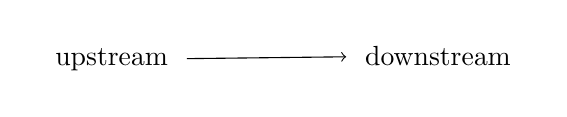
\begin{tikzpicture}
  \matrix (m) [matrix of math nodes, row sep=4.8em, column sep=5.8em, minimum width=2.2em]
  {
\text{ upstream } & \text{ downstream } \\ 
};
  \path[->]
  (m-1-1) edge node [above] {$ $} (m-1-2);
\end{tikzpicture}  \\
 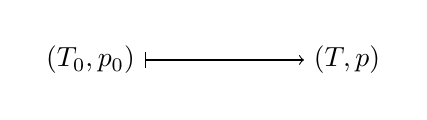
\begin{tikzpicture}
  \matrix (m) [matrix of math nodes, row sep=4.8em, column sep=5.8em, minimum width=2.2em]
  {
(T_0,p_0) & (T,p) \\ 
};
  \path[|->]
  (m-1-1) edge node [auto]  {$$} (m-1-2)
  ;
\end{tikzpicture}   \\
 \frac{T_0}{T} = 1 + \frac{\gamma -1}{2} \mathfrak{M}^2 \\ 
 \frac{p_0}{p} = \left( 1 + \frac{\gamma -1}{2} \mathfrak{M}^2 \right)^{\frac{\gamma}{\gamma -1} }
\end{gathered}
\]

Thus, when one considers heat addition, the thermodynamic process, $\Delta \dot{q}$ occurs on stagnation temperature, and then can be related to the actual, physical fluid flow and its properties, through formulae we've derived: \\
 \begin{tikzpicture}
  \matrix (m) [matrix of math nodes, row sep=4.8em, column sep=5.8em, minimum width=2.2em]
  {
    x_0   \\
    x_1 \\
};
  \path[|->]
  (m-1-1) edge node [auto] {$u$} (m-2-1)
  ;
\end{tikzpicture} 
 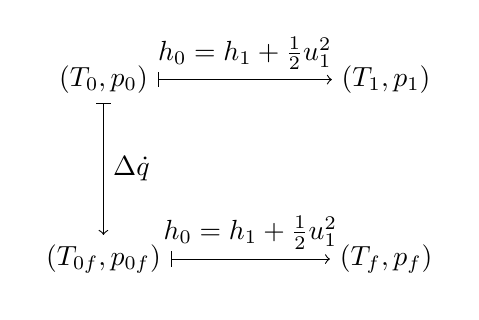
\begin{tikzpicture}
  \matrix (m) [matrix of math nodes, row sep=4.8em, column sep=5.8em, minimum width=2.2em]
  {
    (T_0,p_0) & (T_1,p_1)  \\
    (T_{0f},p_{0f}) & (T_f,p_f) \\ 
};
  \path[|->]
  (m-1-1) edge node [auto] {$h_0 = h_1 + \frac{1}{2}u_1^2$} (m-1-2)
          edge node [auto] {$\Delta \dot{q}$} (m-2-1)
  (m-2-1) edge node [auto] {$h_0 = h_1 + \frac{1}{2}u_1^2$} (m-2-2)
  ;
\end{tikzpicture} 

\begin{lstlisting}
(1.*10**6)/(40.*15.6)
# 1602.5641025641025
\end{lstlisting}
So
\[
\Delta T_0 = 1602.6 \, K
\]
\item[(b)] Now consider the converging section at the inlet to each 1 \, $cm$ diameter channel, that ``accelerates the flow to a relatively low Mach number and produces a flow rate of $40 \, g/s$''.  

Mass continuity (conservation) still holds:
\[
\begin{gathered}
  \dot{m} = \rho A u = \frac{p}{RT} A \mathfrak{M} \sqrt{ \gamma RT } = \frac{p}{\sqrt{RT}} A\mathfrak{M} \sqrt{\gamma } = \frac{p_0 \sqrt{\gamma }}{ \sqrt{RT_0 } } A \mathfrak{M} (1 + \frac{\gamma -1}{2} \mathfrak{M}^2 )^{ \frac{\gamma+1}{-2(\gamma -1) } }
\end{gathered}
\]
where the ``pullback'' to the stagnation properties for each point of the flow, before the converging section and after the converging section, was used:
\[
\begin{aligned}
  & \frac{p_0}{p} = \left( 1 + \frac{\gamma-1}{2} \mathfrak{M}^2 \right)^{\frac{\gamma}{\gamma -1} } \\
  &  \frac{T_0}{T} = 1 + \frac{\gamma-1}{2} \mathfrak{M}^2
\end{aligned}
\]
\begin{lstlisting}
massconsEq = Eq(massflow,p_0*sqrt(gamma/(R*T_0))*A*Mach*(1+(gamma-Rat(1))/Rat(2)*Mach**2)**\
((gamma+1)/(-Rat(2)*(gamma-1))))
massconsProb0503 = massconsEq.subs(massflow,40.*10**(-3)).subs(gamma,1.4).subs(p_0,6.8*10**(6)).\
subs(T_0,673.).subs(A,N(pi)*(10**(-2)/2.)**2).subs(R,k_Boltz.Value/(Decimal(2.0159*10**(-3))/N_Avog.Value))
\end{lstlisting}
where for $R$, $R = \frac{k_B}{M}$ and where for $M$, I used $2.0159 g/\text{mol}$ for \ce{H2}, and Avogadro's number, $N_A = 6.022140857\times 10^{23}$, which is number of particles per mole.  So in this example, $R = 4124.4$ for \ce{H2} as
\begin{lstlisting}
>>> k_Boltz.Value/(Decimal(2.0159*10**(-3))/N_Avog.Value)
Decimal('4124.440627733807619868515695')
\end{lstlisting}

Let's try to use the derived relation, relating the stagnation temperatures before and after (denoted $1$) heat addition:
\[
\frac{T_0}{T_{01}} = \left[ \frac{ 1 + \gamma \mathfrak{M}_1^2 }{1 + \gamma \mathfrak{M}^2}\left( \frac{\mathfrak{M}}{\mathfrak{M}_1}\right)\right]^2\left[\frac{1+\frac{\gamma-1}{2}\mathfrak{M}^2}{1+\frac{\gamma-1}{2}\mathfrak{M_1}^2}\right]
\]
This is implemented in \verb|NozzleTheory.py|:
\begin{lstlisting}
T_01=Symbol('T_01',real=True)
heataddTvsMachEq=Eq(T_0/T_01,((Rat(1)+gamma*Mach_1**2)/(Rat(1)+gamma*Mach**2)*Mach/Mach_1)**2*\
(Rat(1)+(gamma-Rat(1))/Rat(2)*Mach**2)/(1+(gamma-Rat(1))/Rat(2)*Mach_1**2) )

heataddTvsMachProb0503=heataddTvsMachEq.subs(gamma,1.4).subs(T_0,675).subs(T_01,675+(1.*10**6)/\
(40.*15.6)).subs(Mach,MachProb0503)
Mach1Prob0503lamb=lambdify(Mach_1,heataddTvsMachProb0503.rhs-heataddTvsMachProb0503.lhs)
plot(heataddTvsMachProb0503.rhs,(Mach_1,0,10))
Mach1Prob0503=scipy.optimize.newton(Mach1Prob0503lamb,0.1)
\end{lstlisting}
where $\mathfrak{M}$ was obtained for the acceleration by the converging nozzle, $T_0$ is the stagnation temperature that was given, and $T_{01}$ is obtained from part (a).  

Thus,
\[
\mathfrak{M}_1 = 0.2024
\]
The flow through the channel isn't thermally choked as $\mathfrak{M}$ doesn't become $1$ by the heat addition.  
\item[(c)] After exiting the ducts, the converging-diverging nozzle results in a Mach number given by
\[
\frac{A_e}{A^*} = \frac{1}{\mathfrak{M}} \left[ \left( \frac{1 + \frac{\gamma-1}{2} \mathfrak{M}^2 }{ \frac{\gamma+1}{2} } \right)^{\frac{\gamma+1}{\gamma-1} } \right]^{1/2}
\]
and from the Mach number definition and energy equation (Bernoulli invariant), we can get the exhaust velocity
\[
u_e = \mathfrak{M}a = \mathfrak{M}\sqrt{\gamma RT} = \mathfrak{M} \sqrt{ \gamma R \frac{ T_0 }{ 1 + \frac{\gamma-1}{2} \mathfrak{M}^2 } }
\]
\end{enumerate}


\textbf{Hydrazine monopropellant thrusters}

Consider in general 2 reactions of the form 
\[
\sum_j \nu_j A_j = 0 
\]
and 
\[
\xi_K A_K + \sum_k \xi_k B_k = 0 
\]
with the convention that the stoichiometric coefficients ``on the left'' (reactants) are negative integers.  

Clearly, 
\[
\begin{gathered}
  dN_j = \nu_j d\widehat{N} \\ 
  dN_k = \xi_k d\widehat{N}_2
\end{gathered}
\]
where 
\[
\begin{aligned}
  & d\widehat{N} \equiv \text{ how many times reaction 1 takes place } \\ 
  & d\widehat{N}_2 \equiv \text{ how many times reaction 2 takes places }
\end{aligned}
\]
since in chemical reactions, chemical species can't be ``broken down'' or ``destroyed'' into smaller parts (we're not considering nuclear reactions).  

Then for the particular chemical species $A_K$, \[
\begin{aligned}
  & dN_K = \nu_K d\widehat{N} \text{ and } \\
  & dN_{K_2} = \xi_{K_2} d\widehat{N}_2
\end{aligned}
\]  for chemical species $K$ to occur in the second reaction.  Thus, given the fraction $X$ that participates in the second chemical reaction, observe, importantly, that
\[
\begin{gathered}
  XdN_k = -dN_{K_2} = - \xi_{K_2} d\widehat{N}_2 \\
  \frac{-X\nu_K}{\xi_{K_2}} d\widehat{N} = d\widehat{N}_2
\end{gathered}
\]
and so for the other chemical species (molecules) in the second reaction, their ``stoichiometric'' coefficients change in the following manner:
\begin{equation}\label{Eq:stoichiometriccoeffsreaction2}
  dN_k = \xi_k \frac{X \nu_k}{-\xi_{K_2}} d\widehat{N}
\end{equation}
and so writing the first reaction as 
\[
\sum_j \nu_j A_j =0 = \sum_{k \neq K} \nu_k A_k + \nu_K A_K 
\]
then we simply only need to add up reactions 1 and 2, with reaction 2 taking new stoichiometric coefficients according to Eq. \ref{Eq:stoichiometriccoeffsreaction2}:
\begin{equation}\label{Eq:dissociationreactiongeneral}
\boxed{ \sum_{k\neq K} \nu_k A_k + \nu_K(1-X) A_K + \sum_l \frac{ \xi_l X \nu_l }{ -\xi_{K_2} } B_l = 0 }
\end{equation}
Indeed, consider the (exothermic) decomposition of hydrazine and then the dissociation of ammonia into elevated temperatures:
\[
\begin{aligned}
  &  \ce{3N2H4 -> 4NH3 + N2} \\ 
  &  \ce{4NH3 -> 2N2 + 6H2 }
\end{aligned}
\]
Then plugging into our formula, Eq. \ref{Eq:dissociationreactiongeneral}, 
\[
\begin{gathered}
  -3 \ce{N2H4} + 4(1-X) \ce{NH3} + \ce{N2} + \frac{2\cdot X\cdot 4}{4} \ce{N2} + \frac{6 \cdot X \cdot 4}{4} \ce{H2} = 0 = -3 \ce{N2H4} + 4(1-X) \ce{NH3} + (1+2X)\ce{N2} + 6X\ce{H2} \\
\Longrightarrow \boxed{ \ce{N2H4 -> } 4(1-X) \ce{NH3} + (1+2X) \ce{N2} + 6X \ce{H2} }
\end{gathered}
\]
Indeed, for the following limits, 
\[
\begin{aligned}
X \to 0  \qquad \, &  \ce{3N2H4 -> 4NH3 + N2} \\ 
 X \to 1  \qquad \, &  \ce{3N2H4 -> 3N2 + 6H2 }
\end{aligned}
\]

\emph{adiabatic flame temperature}

Remember that for adiabatic processes, $Q=0$, and so $Q=0=\Delta H = H_{\text{products}} - H_{\text{reactants}}$ and so for adiabatic processes, $H_{\text{products}} = H_{\text{reactants}}$, given by 
\begin{equation}
\begin{aligned}
  H_P(\tau_P) = \sum_{i\in \lbrace \text{products}\rbrace } n_i \left[ \Delta_f \overline{h}_i^0 + \overline{h}_i(\tau_P) - \overline{h}_i^0 \right]   \\
  H_R(\tau_R) = \sum_{i\in \lbrace \text{reactants} \rbrace } n_i \left[ \Delta_f \overline{h}_i^0 + \overline{h}_i(\tau_R) - \overline{h}_i^0 \right]
\end{aligned}
\end{equation}
where $P$ denotes products and $R$ denotes reactants.  

The upper bound of the adiabatic flame temperature is given by no dissociation $(X=0)$.  The lower bound of the adiabatic flame temperature is given by the flame temperature with full dissociation $(X=1)$.  

EY : 20160121 My question is this: is this because the dissociation of ammonia is endothermic, as the heat of formation of ammonia is $\Delta H_f^{\circ} = -45.894 \, kJ/\text{mol}$, and so heat is given off in its formation, and so for full dissociation, the temperature goes down.  Is this also because of Le Chatelier's principle?  A clear explanation according to Le Chatelier's principle would also be appreciated.

Remember that the heat of formation for stable elements is $0$.  

For the case of $X=0$, $Q=0$ leads to
\[
\begin{gathered}
  3 \cdot \left[ \Delta_{f;\ce{N2H4}}^{\circ} + 0 \right] = 4 \cdot \left[ \Delta_{f;\ce{NH3}}^{\circ} + (H-H(T^{\circ}))_{\ce{NH3} }  \right]+ 1 \left[ 0 + (H-H(T^{\circ}))_{\ce{N2}} \right]
\end{gathered}
\]

For the case of $X=1$, $Q=0$ leads to
\[
\begin{gathered}
  3 \cdot \left[ \Delta_{f;\ce{N2H4}}^{\circ} + 0 \right] =  3 \left[ 0 + (H-H(T^{\circ}))_{\ce{N2}} \right] +  6 \left[ 0 + (H-H(T^{\circ}))_{\ce{H2}} \right]
\end{gathered}
\]

We were given a quadratic polynomial fit to data taken from JANAF (or JANNAF?) tables for \ce{N2},\ce{H2},\ce{NH3}:
\[
\begin{aligned}
  \ce{N2} \qquad  & H-H(T^{\circ}) = -8.553 + 27.77 \theta + 2.317 \theta^2 \\  
  \ce{H2} \qquad  & H-H(T^{\circ}) = -8.292 + 27.39 \theta + 1.586 \theta^2 \\ 
  \ce{NH3} \qquad & H-H(T^{\circ}) = -10.37 + 31.32 \theta + 11.77 \theta^2
\end{aligned}
\]
where $\theta = T/1000$ and $T$ is in Kelvins ($K$).  

Solving for a quadratic function is easy with \verb|scipy| using the module \verb|optimize| and the method \verb|newton|.  The code is in \verb|combustion.py|.  

The upper bound of the adiabatic flame temperature $T_{ad}$ was found to be
\[
T_{ad} = 1644 \, K = 1371 \, C = 2498 \, F
\]
and the lower bound of the adiabatic flame temperature was found to be 
\[
T_{ad} = 866 \, K = 593 \, C = 1099 \, F
\]

\textbf{Gibbs function for a mixture of gases}

Let $\Sigma$ be a 2-dimensional (i.e. $\text{dim}{\Sigma}=2$) manifold representing all possible thermodynamic states of the system (in this case, of an ideal gas).  Let $\Sigma$ have  coordinates $\tau,p$, representing the temperature $\tau$, and pressure $p$, of the system, respectively, which could've been obtained from (successive) Legendre transformations of (global) coordinates $U, V$, where $U$ is energy.  

Let $Q$, representing heat applied onto, or heat into, the system, be a 1-form of $\Sigma$, i.e. $Q \in \Omega^1(\Sigma)$.  

Then $Q$ can be written, in general, as 
\[
Q = C_p d\tau + \frac{ \partial Q}{ \partial p} dp
\]
Let's determine $\frac{\partial Q}{\partial p}$.  From energy conservation (i.e. ``First law'' of thermodynamics), $Q = dU + pdV$ (i.e. $Q$ in (global) coordinates of $U,V$ for $\sigma$.  Next, consider a curve $\gamma:\mathbb{R}\to \Sigma$ in $\Sigma$, representing a thermodynamic process, such that $d\tau(\dot{\gamma})=0$ which says that the process occurs at constant temperature $\tau$.  Note that $\dot{\gamma}$ is a vector field in $\Sigma$, i.e. $\dot{\gamma} \in \mathfrak{X}(\Sigma)$.  Then
\[
\begin{gathered}
  Q(\dot{\gamma}) = C_p d\tau(\dot{\gamma}) + \frac{ \partial Q}{ \partial p} dp(\dot{\gamma}) = 0 + \frac{ \partial Q}{ \partial p} dp(\dot{\gamma})= dU(\dot{\gamma}) + pdV(\dot{\gamma})
\end{gathered}
\]
For an ideal gas, $U = \frac{1}{\gamma -1} N\tau$ and so $dU = \frac{1}{\gamma-1}Nd\tau$ and so $dU(\dot{\gamma}) = \frac{1}{\gamma -1}Nd\tau(\dot{\gamma}) =0$.  It also sufficed to say that for an ideal gas, $U=U(\tau)$, i.e. $U$ is only a function of temperature, and so $U$ is constant during a process where temperature remains constant. 

Then, using $pV=N\tau$ which must always hold for an ideal gas in equilibrium, 
\[
V= \frac{N\tau}{p} \Longrightarrow dV = \frac{N\tau}{-p^2} dp
\]
and so 
\[
\frac{ \partial Q}{ \partial p } dp = 0 + p\left( \frac{N\tau}{-p^2} \right)dp = \frac{-N\tau}{p} dp = -Vdp
\]
Thus $\frac{\partial Q}{ \partial p} = -V$.  One can (physically) interpret this as showing how heat, applied to this ideal gas system, can cause our system to be able to do (physical) work.  

Then equating $Q = \tau d\sigma$, 
\[
\begin{gathered}
\tau d\sigma = Q = C_p d\tau - V dp \Longrightarrow d\sigma = \frac{C_p}{\tau}{d\tau}  - \frac{V}{\tau} dp = \frac{C_p d\tau}{\tau} - \frac{N dp}{p}
\end{gathered}
\]
Taking the integral,
\[
\sigma -\sigma_0 = \int_{\tau_0}^{\tau} \frac{C_p d\tau}{\tau} - N\ln{ \frac{p}{p_0} }
\]
Let's talk about, for a mixture of ideal gases,  partial pressures $p_i$ for each of the (kinds of) species $i$.  It makes (physical) sense that the contribution to the total pressure $p$ from a single species labeled $i$ would be proportional to the number of particles $N_i$ of the species $i$ (imagine (infinitesimally small) colliding billiard balls).  Then $p_i = \frac{N_i}{N} p$ and so 
\[
N_i \ln{ \frac{p_i}{p_0} } = N_i \ln{ \frac{N_i p}{Np_0} } = N_i \ln{ \frac{p}{p_0}} + N_i \ln{ \frac{N_i}{N} }
\]
For a mixture of ideal gases, there is no interaction energy (by definition of \emph{ideal}), and so entropies are \emph{additive} \cite{LLandauELifshitz1980}.  So 
\[
\begin{gathered}
  \sigma = \sum_i \sigma_i = \sum_i \left( \int_{\tau_0}^{\tau} \frac{C_{pi} d\tau }{\tau} + \sigma_{i0} \right) - N \ln{ \frac{p}{p_0} } - \sum_i N_i \ln{ \frac{N_i}{N} }
\end{gathered}
\]
$\sigma$ in its current state is unitless.  Multiply by the Boltzmann constant $k_B$ and Avogadro's number $N_A$ as appropriate to obtain the desired units for entropy $S$.  

\subsubsection{ig thermo.xls; Dealing with tables}

Doing a search on Google for \verb|ig_thermo.xls| yields this link: \\
\url{http://www.google.com/url?q=http://shepherd.caltech.edu/EDL/projects/pde/ig_thermo.xls&sa=U&ved=0ahUKEwjt2ta8x7nKAhVB8GMKHa-tCBYQFggUMAA&usg=AFQjCNGcu2ryEOaIZqwumHooxDjcxTf3gQ}

However, ammonia is not to be found in \verb|ig_thermo.xls| \emph{off the Web}.  

Let's consider the work-flow or process of scraping the NIST website for JANAF table data.  Starting from the \href{http://kinetics.nist.gov/janaf/}{NIST-JANAF Thermochemical Tables} webpage, one can enter, as a string, the CAS number, chemical formula, or compound name, or search by the periodic table.  However, using the periodic table, for element \ce{N} or \ce{H}, ammonia wasn't to be found (as of 20160120).  However, entering \ce{NH3} or Ammonia (the search text box ``field'' is case-sensitive), leads to the ammonia gas JANAF table.  Then one clicks on the link for ``\href{http://kinetics.nist.gov/janaf/html/H-083.html}{view}'' for the HTML-formatted table and then follow the bottom link for the tab-separated table.  

So it would be nice to do the following:
\begin{itemize}
  \item Obtain a \emph{comprehensive} list of all available compounds of this NIST JANAF database and with that 
  \item scrape all the tab-separated tables.  
\end{itemize}
A comprehensive list appears to be in this pdf link for \href{http://kinetics.nist.gov/janaf/pdf/JANAF-FourthEd-1998-1Vol1-Intro.pdf}{Volume 1} of the JANAF tables.  Perhaps this pdf could be ``scraped'' to obtain a list of compounds in text format?  



\subsubsection{entropy of a mixture of ammonia, nitrogen, and hydrogen}

Recall that 
\[
\ce{N2H4 -> } 4(1-X) \ce{NH3} + (1+2X) \ce{N2} + 6X \ce{H2}
\]
and that we had derived
\[
S(T,P) = \sum_i N_i \left( \int_{T_0}^T c_{pi} \frac{dT}{T} + s_{i0} \right) - NR \ln{ \frac{P}{P_0} } - R \sum_i N_i \ln{ \frac{N_i}{N} }
\]

The values we want are for $P = 1 \, \text{atm}$ and $P=10 \, \text{atm}$  

Note that 
\[
N=4(1-X) + (1+2X) + 6X = 4X +5
\]
and 
\[
\sum_i N_i \ln{\frac{N_i}{N} } = 4(1-X) \ln{ \left( \frac{4(1-X)}{4X+5} \right) } + (1+2X)\ln{ \left( \frac{1+2X}{4X+5} \right) } + 6X \ln{ \left( \frac{6X}{4X+5} \right) }
\]


\section{Equilibrium flow vs. frozen flow for Nozzle Flow and the Example of the Space Shuttle Main Engine (SSME)}

\begin{enumerate}
  \item Remember that from Newton's 2nd law, the so-called momentum equation, is 
\[
  \rho \frac{Du}{Dt}  = \text{div}(\mathbf{T}) \text{ or } \rho \left[ \frac{ \partial \mathbf{u} }{ \partial t} + u^j \frac{ \partial \mathbf{u} }{ \partial x^j} \right] = \text{div}(\mathbf{T})
\]

Let 
\begin{equation}
  k := \frac{1}{2} \rho u^2 
\end{equation}
which is a scalar quantity that depends on time $t$ and spatial coordinates $\mathbf{x} = (x^1 \dots x^n) \in N$ and represents the density of kinetic energy of the bulk fluid at time $t$ and spatial point $\mathbf{x}$.  

Clearly, product rule still applies when using the material derivative $\frac{D}{Dt}:= \frac{ \partial }{ \partial t} + u^j \frac{ \partial }{ \partial x^j}$:
\[
\begin{gathered}
  \frac{D}{Dt} k =\frac{D}{Dt} \frac{1}{2} \rho u^2 = \frac{1}{2} \left[ u^2 \frac{D\rho }{Dt} + \rho \left( \frac{D}{Dt} u^2 \right)\right] = \frac{1}{2} \left[ u^2 (-\rho \text{div}u ) + \rho \left( \frac{D}{Dt} u^2 \right) \right]
\end{gathered}
\]
If, say, $g = 1$, then $u^2 = u_i u^i = (u^i)^2$, and so 
\[
\begin{gathered}
 \rho \frac{D}{Dt} u^2 = 2\rho u^i \frac{D}{Dt} u^i = 2 u^i \text{div}(T^i)
\end{gathered}
\]
and so in this case,
\[
\frac{D}{Dt} k = \frac{-1}{2} \rho u^2 \text{div}(u) + u^i \text{div}(T^i) = -k \text{div}(u) + u^i \text{div}(T^i)
\]
and since
\[
u^j \frac{ \partial k}{ \partial x^j} + k\text{div}(u) = \text{div}(ku)
\]
then we could also write
\[
\frac{D}{Dt}k + k \text{div}(u) = \frac{ \partial k}{ \partial t } + \text{div}(ku) = u^i \text{div}(T^i)
\]

What about the case where $g \neq 1$ but could be dependent upon time and space?  

Invoke the ``Fundamental Theorem on Time-Dependent Flows'' (Theorem 9.48 in Chapter 9 Integral Curves and Flows, pp. 237 of Lee (2012) \cite{JLee2012}, which guarantees the existence of a time-dependent flow $\phi$ for our velocity vector field $\mathbf{u}$.  

So for our time-dependent velocity vector field, $\mathbf{u} \in \mathfrak{X}(\mathbb{R}\times N)$, i.e.
\[
\begin{aligned}
  & \mathbf{u}: \mathbb{R} \times N \to TN \\
  & \mathbf{u} = \mathbf{u}(t,\mathbf{x}) = u^i(t,\mathbf{x}) \frac{ \partial }{ \partial x^i}
\end{aligned}
\]
there exists a flow, given initial conditions, $\phi = \phi(t) \in N$, such that 
\[
\begin{aligned}
  & \phi(t) = (x^1(t) \dots x^n(t) ) \\ 
  & \dot{\phi}(t) = (\dot{x}^1(t) \dots \dot{x}^n(t)) = (u^1 \dots u^n)
\end{aligned}
\]
Thus, again emphasizing on any Riemannian manifold $(M,g)$, equipped with metric $g$,
\[
u^2 = g_{ij} u^i u^j = g_{ij} \dot{\phi}^i \dot{\phi}^j
\]

Consider any time and space dependent scalar quantitiy, $f$, $f \in C^{\infty}(\mathbb{R}\times N)$, i.e. $f:\mathbb{R}\times N \to \mathbb{R}$.  On a flow $\phi$ for a time-dependent vector field $\mathbf{u}$ generating this flow,
\[
\begin{gathered}
  \frac{d}{dt}f = \frac{d}{dt}f(t,\mathbf{x}) = \frac{d}{dt}f(t,\mathbf{x}(t)) = \frac{ \partial }{ \partial t}f + \frac{ \partial f}{ \partial x^i} \dot{x^i} = \frac{ \partial }{ \partial t} f + u^i \frac{ \partial f}{ \partial x^i} =  \\
  = \frac{D}{Dt}f
\end{gathered}
\]
Thus, in this scenario, then $\forall \, f \in C^{\infty}(\mathbb{R}\times N)$, the material derivative $\frac{D}{Dt}$ of $f$ is equal to the total time derivative $\frac{d}{dt}$.  

Then for scalar quantity $u^2 = u^2(t,\mathbf{x}) = g_{ij}(\phi(t)) \dot{\phi}^i \dot{\phi}^j$, 
\[
\frac{d}{dt} u^2 = \frac{ \partial g_{ij}}{ \partial x^k } \dot{\phi}^k \dot{\phi}^i \dot{\phi}^j + 2 g_{ij} \dot{\phi}^i \ddot{\phi}^j = 2 g_{ks} \Gamma_{ij}^k \dot{\phi}^i \dot{\phi}^j \dot{\phi}^s + 2 g_{sk} \dot{\phi}^s \dot{\phi}^k = 2g_{ks} \dot{\phi}^s \left[ \ddot{\phi}^k + \Gamma^k_{ij} \dot{\phi}^i \dot{\phi}^j \right]
\]
where the identity
\[
\frac{ \partial g_{ij} }{ \partial x^k} \dot{\phi}^k \dot{\phi}^i \dot{\phi}^j = 2 g_{ks} \Gamma^k_{ij} \dot{\phi}^i \dot{\phi}^j \dot{\phi}^s
\]
was used, which is in the proof for Theorem 3.25 on pp. 49 of section 3.8 The natural Lagrangian on manifolds of Calin and Chang (2005) \cite{OCalinDChang2005}.  I want to remark that Calin and Chang (2005) \cite{OCalinDChang2005} has explicit computations showing this identity to be the case locally, and at least for me, I don't see many other sources that are this thorough with presenting explicit computations.  

Noting that 
\[
\nabla_u u = \nabla_{u^j \frac{ \partial }{ \partial x^j} } u = u^j \nabla_{\frac{\partial }{ \partial x^j} } u = u^j \left( \frac{ \partial u^k}{ \partial x^j} + \Gamma^k_{ij} u^i \right) \frac{ \partial }{ \partial x^k} = \left( \ddot{\phi}^k + \Gamma^k_{ij} \dot{\phi}^i \dot{\phi}^j \right) \frac{ \partial }{ \partial x^k}
\]
and so
\[
\begin{gathered}
g_{ks}\dot{\phi}^s \left[ \ddot{\phi}^k + \Gamma^k_{ij} \dot{\phi}^i \dot{\phi}^j \right] = \langle u , \nabla_uu\rangle \Longrightarrow \frac{d}{dt}u^2 = 2 \langle u , \nabla_u u \rangle
\end{gathered}
\]
Thus, in general (on a Riemannian manifold), 
\begin{equation}\label{Eq:KEdensityflow}
\boxed{ \frac{\partial k}{\partial t} + \text{div}(ku) = \frac{Dk}{Dt} + k\text{div}(u) = \rho \langle u, \nabla_u u \rangle = \langle u, \text{div}(T) \rangle }
\end{equation}

Now when following a volume element $\text{vol}^n$, along the flow of the fluid, one should be concerned that in a ``lab frame'', the volume itself can change with time:
\[
\begin{gathered}
  \dot{V} = \frac{d}{dt} \int_V \text{vol}^n = \int_V \mathcal{L}_{ \frac{\partial }{ \partial t} + \mathbf{u} } \text{vol}^n = \int_V 0 + \mathcal{L}_{\mathbf{u}} \text{vol}^n = \int_V (\mathbf{d}i_{\mathbf{u}} + i_{\mathbf{u}} \mathbf{d} ) \text{vol}^n = \int_V\mathbf{d}i_{\mathbf{u}} \text{vol}^n + 0 = \\
  = \int_{\partial V} i_{\mathbf{u}} \text{vol}^n = \int_{ \partial V} u^j dS_j
\end{gathered}
\]
Indeed, if the time-dependent velocity vector field $\mathbf{u}$ changes at the boundary $\partial V$, then so does our volume, in this frame.  

The correct way out of this conundrum is to switch to the frame where the bulk velocity of the fluid is $0$, so it's at rest in this frame.  This is paramount to choosing $\mathbf{u}=0$ above, and so $\dot{V}=0$.  

The strategy is this: one should recognize that number of particles $N$, or in general, number of particles for species $i$, $N_i$ and entropy $\sigma$ are invariants under Galilean (or Lorentz) transformation: observers, whether in the lab frame, or the frame in which the bulk velocity of the fluid is $0$ so the bulk fluid flow is at rest, or any other frame, must agree upon these numbers (that can be objectively measured).  So we've fixed our ``control volume'' that remains constant in time in this fluid-at-rest frame, and count the number of particles that come in, and the entropy.  

For only 1 kind of particle, let 
\[
\begin{aligned}
  & \check{\sigma} \equiv \sigma/N \text{ entropy per particle } \\ 
  & \check{\epsilon} \equiv E/N \text{ energy per particle }
\end{aligned}
\]
Thus
\[
\tau d\sigma = \tau d(N \check{\sigma}) = \tau N d\check{\sigma} + \tau \check{\sigma} dN
\]
where 
\[
\begin{aligned}
  & \tau N d\check{\sigma} \text{ is entropy change due to change in entropy per particle, i.e. \textbf{ conduction term } } \\
  & \tau \check{\sigma} dN \text{ is entropy change due to change in number of particles, i.e. \textbf{ convection term } }
\end{aligned}
\]
Generalizing this to $\mathcal{N}$ species, indexed by $i=1\dots \mathcal{N}$, 
\[
\begin{aligned}
  & \check{\sigma}_i \equiv \sigma_i/N_i \text{ entropy per particle of species $i$ } 
\end{aligned}
\]
Assuming that entropies are additive (which is a reasonable assumption if the interaction between species is negligible \cite{LLandauELifshitz1980}), then for total entropy of the system in volume $V$ in this fluid-at-rest frame (which will be denoted with prime as needed), 
\[
\sigma = \sum_i \sigma_i = \sum_i \check{\sigma}_i N_i
\]
So
\[
\tau d\sigma = \tau \sum_i N_i d\check{\sigma}_i + \tau \sum_i \check{\sigma}_i dN_i
\]
where 
\[
\begin{aligned}
  & \tau \sum_i N_i d\check{\sigma}_i \text{ is entropy change due to change in entropy per particle for each species, i.e. \textbf{ conduction term } } \\
  & \tau \sum_i \check{\sigma}_i dN_i \text{ is entropy change due to change in number of particles for each species, i.e. \textbf{ convection term } }
\end{aligned}
\]
Using the above result for the decomposition of $\tau d\sigma$ into a conduction term and convection term, then
\begin{equation}\label{Eq:dEconductionconvectiondecomposition}
\begin{gathered}
  dE = \tau d\sigma - p dV + \sum_i \mu_i dN_i = \tau \sum_i N_i d\check{\sigma}_i + \tau \sum_i \check{\sigma}_i dN_i - pdV + \sum_i \mu_i dN_i = \\
  = \tau \sum_i N_i d\check{\sigma}_i + \sum_i ( \tau \check{\sigma}_i + \mu_i ) dN_i - pdV = \tau \sum_i N_i d\check{\sigma}_i + \sum_i \check{h}_i dN_i - pdV = \tau \sum_i N_i d\check{\sigma}_i + \sum_i \check{h}_i dN_i 
\end{gathered}
\end{equation}
since $dV=0$ for any thermodynamic process in this constant volume and that
\[
G_i = F_i + p_iV = E_i - \tau \sigma_i + p_i V = H_i - \tau \sigma_i = \mu_i N_i \Longrightarrow \check{h}_i = \mu_i + \tau\check{\sigma}_i
\]
since Gibbs free energy $G_i$ for each species $i$ should be additive, partial pressures $p_i$ for each species $i$ should be additive to the total pressure $p$, as forces are additive, and from the definition of enthalpy $H_i = E_i + p_iV$ for each species $i$.  

For the case of 1 species, and for this volume at rest in the fluid-at-rest frame, $V$, then defining
\[
\begin{aligned}
  & h := \frac{H}{V} \\
  & s := \frac{\sigma}{V} \\
  & \epsilon := \frac{E}{V}
\end{aligned}
\]
and so from Eq. \ref{Eq:dEconductionconvectiondecomposition},
\[
\begin{gathered}
  d\epsilon  = \tau \frac{N}{V} d\left( \frac{\sigma}{N} \right) + \frac{H}{N} d\left( \frac{N}{V} \right) = \tau \frac{N}{V} \left( \frac{d\sigma}{N} + -\frac{ \sigma dN}{ N^2 } \right) + \frac{H}{N} \frac{d\sigma}{M} = \tau ds - \frac{\tau s}{\rho} d\rho + \frac{h d\rho}{\rho} = \tau ds + \frac{h-\tau s}{ \rho} d\rho 
\end{gathered}
\]
We should denote with prime symbols ($'$) the quantities that transform under change of observer's frame, and is specific, in value, to this fluid-at-rest frame:
\[
d\epsilon' = \tau ds + \frac{h'-\tau s}{\rho} d\rho
\]
For many species, then generalizing the above,
\[
d\epsilon' = \tau \sum_i \frac{N_i}{V} d\left( \frac{\sigma_i}{N_i} \right) + \sum_i \frac{H_i}{N_i}d\frac{N_i}{V} = \tau \sum_i \frac{N_i}{V} \left( \frac{d\sigma_i}{N_i} + - \frac{\sigma_i dN_i}{N_i^2} \right) + \sum_i \frac{h_i'}{\rho_i}d\rho_i = \tau ds + \sum_i \frac{ h_i' - \tau s_i }{\rho_i} d\rho_i 
\]

Thus, in this fluid-at-rest frame,
\begin{equation}\label{Eq:internalenergyfluidatrest}
  \boxed{ d\epsilon' = \tau ds + \sum_i \frac{h_i'-\tau s_i}{\rho_i} d\rho_i}
\end{equation}

Next, use the fact that for a fluid in the ``lab frame'', the current density for the total energy $E$ is carried by $(k+h')\mathbf{u}$ and \emph{not} $(k+\epsilon')\mathbf{u}$.  This comes from the fact that for compressible flows, the Bernoulli invariant is $k+h' = \frac{1}{2} \rho u^2 + h'$, and not $k+\epsilon'$.  The physical interpretation is that the enthalpy $h'$ is needed to account for all convection terms, to account for the ``energy balancing'' needed, done by the compression of the volume by $vdN_i := V/N_i dN_i$ to return to the initial volume $V$ in the fluid-at-rest frame, when particles of species $i$ flow through the volume $V$, convection.  

Thus
\begin{equation}\label{Eq:totalenergyfluxbyenthalpy}
\begin{gathered}
  \frac{ \partial \epsilon }{ \partial t} + \text{div}( (k+h')\mathbf{u} ) = 0 \text{ or } \frac{ \partial \epsilon }{ \partial t} + \text{div}(ku) = -\text{div}(h'u)
\end{gathered}
\end{equation}

With all these ingredients, begin with the account of all energies in the lab frame, for a fluid:
\[
E= KE + U \Longrightarrow \epsilon = k + \epsilon' \Longrightarrow \frac{ \partial \epsilon }{ \partial t} = \frac{ \partial k }{ \partial t} + \frac{ \partial \epsilon'}{ \partial t}
\]
From Eq. \ref{Eq:KEdensityflow}, to substitute into $\frac{ \partial k}{ \partial t}$, 
\[
\frac{ \partial \epsilon}{ \partial t} = -\text{div}(ku) + \langle u, \text{div}T \rangle + \frac{ \partial \epsilon'}{ \partial t}
\]
From Eq. \ref{Eq:internalenergyfluidatrest}, we can consider a thermodynamic process where we vary the time, generated by vector $\frac{ \partial }{ \partial t}$, so that we have
\[
\frac{ \partial \epsilon'}{ \partial t} = \tau \frac{ \partial s}{ \partial t} + \sum_i \frac{h_i'-\tau s_i}{\rho_i} \frac{ \partial \rho_i}{ \partial t}
\]
and so 
\[
\frac{ \partial \epsilon}{ \partial t} = -\text{div}(ku) + \langle u, \text{div}T \rangle + \tau \frac{ \partial s}{ \partial t} + \sum_i \frac{h_i'-\tau s_i}{\rho_i} \frac{ \partial \rho_i}{ \partial t} = -\text{div}(ku) - \text{div}(h'u)
\]
where in the last equality, we used Eq. \ref{Eq:totalenergyfluxbyenthalpy}.  Eliminating $-\text{div}(ku)$ from both sides, noting that 
\[
\text{div}(h'u) = \frac{1}{\sqrt{g}} \frac{ \partial (h'u^j \sqrt{g} )}{ \partial x^j} = u^j \frac{ \partial h'}{ \partial x^j} + h'\text{div}(u)
\]
and using $T = -p1$, the case where the stress tensor is only the isotropic (same in all directions) pressure $p$, then
\begin{equation}\label{Eq:provingisentropicflow}
-u^j \frac{ \partial p}{ \partial x^j} + \tau \frac{ \partial s}{ \partial t} + \sum_i \frac{ h_i' - \tau s_i}{ \rho_i} \frac{ \partial \rho_i}{ \partial t} =  - u^j \frac{ \partial h'}{ \partial x^j} - h'\text{div}(u)
\end{equation}
Now we'll need to use a mass conservation law for each of the species $i$, which I'm not sure is valid (please correct me if I'm wrong):
\[
\frac{ \partial \rho_i}{ \partial t} + \text{div}(\rho_i u) =0 \Longrightarrow \frac{ \partial \rho_i}{ \partial t} = - \rho_i \text{div}u - u^j \frac{ \partial \rho_i}{ \partial x^j}
\]
and so
\[
\begin{gathered}
  \sum_i \frac{ h_i' - \tau s_i}{ \rho_i} \frac{ \partial \rho_i}{ \partial t} = \sum_i -h_i' \text{div}u + \tau s_i \text{div}u - \frac{ h_i' - \tau s_i }{ \rho_i} u^j \frac{ \partial \rho_i}{ \partial x^j} = -h' \text{div}u + \tau s \text{div}u - \sum_i \frac{ h_i' - \tau s_i }{ \rho_i} u^j \frac{ \partial \rho_i}{ \partial x^j}
\end{gathered}
\]
Plugging this into Eq. \ref{Eq:provingisentropicflow}, 
\[
\begin{gathered}
  -u^j \frac{ \partial p}{ \partial x^j} + \tau \frac{ \partial s}{ \partial t} + -h' \text{div}u + \tau s \text{div}u - \sum_i \frac{ h_i' - \tau s_i }{ \rho_i} u^j \frac{ \partial \rho_i}{ \partial x^j}  =  - u^j \frac{ \partial h'}{ \partial x^j} - h'\text{div}(u)
\end{gathered}
\]
Noting that by definition, $h':= H'/V = \epsilon' +p$
Using Eq. \ref{Eq:internalenergyfluidatrest} one more time so that
\[
 \frac{ \partial \epsilon'}{ \partial x^j} u^j= \left[ \tau \frac{ \partial s}{ \partial x^j} + \sum_i \frac{h_i'-\tau s_i}{\rho_i} \frac{ \partial \rho_i}{ \partial x^j} \right]u^j
\]
and thus
\[
\tau \frac{ \partial s}{ \partial t} + \tau s\text{div}u + \tau u^j \frac{ \partial s }{ \partial x^j} = 0 \Longrightarrow \boxed{ \frac{ \partial s}{ \partial t} + \text{div}(su) }
\]
Thus, entropy is conserved over time.  Indeed
\[
\dot{S} = \frac{d}{dt} \int_V s \text{vol}^n = \int_V \left( \frac{ \partial s}{ \partial t} + \text{div}(su)  \right) \text{vol}^n
\]
Also notice that I did not assume incompressibility.  This, and the statements above, are true for compressible and incompressible flow.  Also, note that all the above was proven for any Riemannian manifold $N$ representing space.  \item I supposed the reaction was \[
\begin{gathered}
  \ce{2H2 + O2 -> 2H2O }   
\end{gathered}
\]
But the reaction listed for \verb|h2o2.cti| or \verb|h2o2_highT.cti| is 
\[
\ce{H2 + O2 -> H + HO2 }
\]
\end{enumerate}

\section{Liquid-Vapor Equilibrium}

From \href{https://en.wikipedia.org/wiki/Clausius–Clapeyron_relation}{wikipedia}'s article on ``Clausius-Clapeyron relation'', start from the definition of particle diffusion equilibrium, that 
\[
\begin{aligned}
  \mu_v & = \mu_l \\
  d \mu_v & = d \mu_l
\end{aligned}
\]
Using the Gibbs-Duhem relation for each side of the above, that $N d\mu = Vdp - \sigma d\tau$, then
\[
\begin{aligned}
  & d\mu_v = v_v dp- s_v d\tau \\ 
  & d\mu_l = v_l dp- s_l d\tau
\end{aligned}
\]
Thus
\[
(v_v - v_l) dp = (s_v - s_l) d\tau \Longrightarrow \boxed{ \frac{dp}{d\tau} = \frac{s_v - s_l }{ v_v - v_l } }
\]
Using the definition of enthalpy $H:= U + pV$, so that 
\[
dH = dU + Vdp + pdV = \tau d\sigma + Vdp \text{ or } \frac{1}{\tau} ( dH - Vdp) = d\sigma
\]
where $\tau d\sigma = dU + pdV$ was used.  

Considering the thermodynamic process at constant pressure $dp=0$ that begins with a single molecule being in a liquid state and changing into vapor state, then
\[
\frac{1}{\tau} (\Delta H_v) = \sigma_v - \sigma_l
\]
Thus
\[
\frac{dp}{dT} = \frac{ \Delta H_v}{ T (V_v-V_l ) } \approx \frac{\Delta H_v}{ TV_v}
\]
since it's reasonable to assume that the volume of the vapor molecule is much greater than when the molecule is in a liquid state.  

Using the ideal gas law for a single molecule, $pV = \tau$, then
\[
\begin{gathered}
  \frac{dp}{dT} = \frac{ p\Delta H_v}{T^2} \text {or } \frac{dp}{p} = \frac{\Delta H_v dT}{T^2} \\
  \Longrightarrow p(T) = p_0 \exp{ \left( \frac{- \Delta H_v}{T} \right) }
\end{gathered}
\]


\part{Basic Feeling}

\section{Box with a hole rocket; bottled (box) rocket}

Recall Ch. 14: Kinetic Theory, Section ``Kinetic Theory of the Ideal Gas Law'' of Kittel and Kroemer \cite{CKittelHKroemer1980}.

\subsection*{Kinetic Theory of the Ideal Gas Law}

Consider molecule strike unit area of wall. \\
Let $v_z \equiv $ velocity component normal to plane of wall. \\
Suppose molecules, of mass $M$, reflected specularly (mirror-like) from wall,
\[
\Delta p_z = -2M|v_z|
\]
Let $a(v_z)dv_z$, number of molecules per unit volume with $z$-component of velocity between $v_z$ and $v_z + dv_z$.  
\[
\int a(v_z)dv_z = \frac{N}{V} = n
\]
$a(v_z) v_z dv_z$ number of molecules in $(v_z, v_z + dv_z)$  velocity range that strike unit area of wall in (per) unit time
\[
\text{pressure } p = \int_0^{\infty}2M v_za(v_z)v_z dv_z = M\int_{-\infty}^{\infty}v_z^2 a(v_z) dv_z = Mn\langle v_z^2 \rangle
\]
$\frac{1}{2}M\langle v_z^2 \rangle = \frac{1}{2} \tau$ by equipartition of energy (Ch.3)
\[
p = nM \langle v_z^2 \rangle = n\tau = \frac{N\tau}{V}
\]
\subsubsection*{Maxwell Distribution of Velocities}  

cf. Ch.6. distribution function of ideal gas $f(\epsilon_n) = \lambda \exp{ \left( \frac{-\epsilon_n}{\tau} \right)}$

Recall, Ch. 6, Sec. ``Classical Limit'' of Kittel and Kroemer \cite{CKittelHKroemer1980}, \textbf{an ideal gas is defined as a system of free noninteracting particles in the classical regime}.  \\
$f(\epsilon) \equiv $ average occupancy of an orbital at energy $\epsilon$ \\
$\epsilon \equiv $ energy of orbital occupied by 1 particle; not energy of system of $N$ particles \\
Fermi-Dirac and Bose-Einstein distribution $f(\epsilon) = \frac{1}{ \exp{ [ (\epsilon - \mu )/\tau ] } \pm 1 }$ \\
In order for $f(\epsilon) \ll 1$ $\forall \, $ orbitals, $\exp{ [ (\epsilon-\mu)/\tau ] } \gg 1\, \forall \, \epsilon$.  
\[
\Longrightarrow f(\epsilon) \simeq \exp{ [(\mu - \epsilon )/\tau]} = \lambda \exp{ (-\epsilon/\tau)} \quad \, \lambda \equiv \exp{ \left( \frac{ \mu }{\tau} \right) }
\]
$f(\epsilon)$, average occupancy of orbital of energy $\epsilon$, is classical distribution function.  

particle in a box: $\epsilon_n = \frac{1}{2M} \left( \frac{\pi n}{L} \right)^2 $ (for, recall $\frac{1}{2M} \left( \frac{1}{i} \partial \right)^2 \psi = \frac{-1}{2M} \partial^2 \psi = E \psi$)

number of orbitals in range of quantum number $(n,n+dn)$, probability such orbital is occupied

\[
(\frac{1}{2} \pi n^2 dn)f(\epsilon_n) = \frac{1}{2} \pi n^2 \lambda \exp{ (-\epsilon_n/\tau) } dn
\]
\[
\frac{1}{2} Mv^2 = \frac{1}{2M} \left( \frac{ \pi n}{ L } \right)^2 \text{ or } n^2 = \frac{ (ML)^2 }{ \pi^2} v^2 \text{ or } n = \frac{MLv}{\pi}
\]

Consider system of $N$ particles in volume $V$.  

Let $NP(v) dv$ number of atoms with velocity magnitude in range $dv$ at $v$
\[
NP(v) dv = \frac{1}{2} \pi n^2 \lambda \exp{ ( -\epsilon_n /\tau)} \frac{dn}{dv} dv = \frac{1}{2} \pi \lambda \left( \frac{ ML }{ \pi } \right)^3 v^2 \exp{ \left( \frac{ -Mv^2 }{2\tau } \right) }dv
\]
cf. Ch. 6, $\lambda = \frac{n}{n_Q} = \frac{N}{L^3} \left( \frac{ 2\pi \hbar^2 }{ M \tau } \right)^{3/2}$

\[
\frac{1}{2} \pi \frac{N}{L^3} \left( \frac{2\pi }{ M \tau} \right)^{3/2} \left( \frac{ ML }{\pi } \right)^3 = 4\pi N \left( \frac{N}{2\pi \tau} \right)^{3/2}
\]
\begin{equation}
\Longrightarrow P(v) = 4\pi \left( \frac{M}{2\pi \tau } \right)^{3/2} v^2 \exp{ \left( \frac{- Mv^2}{ 2\tau } \right) } 
\end{equation}
$P(v)$ is \textbf{Maxwell velocity distribution}, $P(v)dv$ is probability particle has speed in $dv$ at $v$

\subsubsection*{Experimental verification}

velocity distribution of atoms which exit from slit of oven.  

exit beam weighted in favor of atoms of high velocity at expense of those at low velocity. 

weight factor is velocity component $v\cos{\theta}$ normal to plane of hole. 

\[
\begin{gathered}
  \int (\cos{\theta}) dr rd\varphi r \sin{\theta} d\theta = (\frac{1}{3} (2\pi ) R^3) \int \cos{\theta} \sin{\theta} d\theta = ( \frac{2\pi}{3} R^3) \int \frac{\sin{2\theta} d\theta}{ 2 } = \frac{2\pi R^3}{3} \left. \left( \frac{ - \cos{2\theta} }{4} \right) \right|_0^{\pi/2} = \\
  = \frac{ 2\pi R^3}{3} \left( \frac{1+ 1}{4} \right) = \frac{ 2\pi R^3}{3} \left( \frac{1}{2} \right)
\end{gathered}
\]
Probability atom leaves hole will have velocity in $(v,v+dv)$ : $P_{\text{beam}}(v) dv$

\[
P_{\text{beam}}(v) \propto vP_{\text{Maxwell} } \propto v^3 \exp{ \left( \frac{ -Mv^2}{ 2\tau } \right) }
\]
with, recall $P_{\text{Maxwell}} = 4\pi \left( \frac{ M }{ 2\pi \tau } \right)^{3/2} v^2 \exp{ \left( \frac{-Mv^2}{ 2\tau } \right) }$ 

$P_{\text{beam}}$ distribution of transmission through a hole is Maxwell transmission distribution. 

\begin{equation}\label{Eq:meanvofairbeamouthole}
\begin{gathered}
  \langle v_{\text{out}} \rangle = \int \int_0^{\pi/2} v\cos{\theta} \sin{\theta} d\theta P_{\text{Maxwell}}(v) dv = 4\pi \left( \frac{ M}{ 2\pi \tau} \right)^{3/2} \frac{1}{2} \int_0^{\infty} v^3 \exp{ \left( \frac{-M}{2\tau} v^2 \right) } dv = \\
  = 4\pi \left( \frac{M}{2\pi \tau} \right)^{3/2} \frac{1}{2} \left( \frac{1}{-2\alpha} \right) \left[ 0 - \frac{1}{\alpha} \right] = 4\pi \left( \frac{ M}{2\pi \tau} \right)^{3/2} \frac{1}{4} \left( \frac{4\tau^2}{M^2} \right) = \boxed{ \frac{ 2^{1/2} }{ \pi^{1/2} } \left( \frac{\tau}{M} \right)^{1/2} }
\end{gathered}
\end{equation}
for (doing the integration by hand) 
\[
\begin{aligned}
  & (e^{-\alpha v^2} )' = -2\alpha v e^{-\alpha v^2} \\
  & (v^2 e^{-\alpha v^2} )' = -2\alpha v^3 e^{-\alpha v^2} + 2v e^{-\alpha v^2} \\ 
  & (v^2 e^{-\alpha v^2} + \frac{e^{-\alpha v^2} }{ \alpha } )' = -2\alpha v^3 e^{-\alpha v^2}
\end{aligned}
\]

Armed with this mean velocity $\langle v_{\text{out}} \rangle$ out of a hole of a box, we want the \emph{thrust} that results on a box if we had a box of air, at some pressure, and at some temperature, and then we punch a hole at one end.  

What's happening?  Air that's swirling around the box is then accelerated out of the hole.  There's fluid flow out.  For low enough velocities, use \emph{Bernoulli's equation}, and assume at the starting point of the air's streamline, the velocity is $0$:
\[
\begin{gathered}
  \frac{1}{2} u^2 + \frac{p}{\rho} = \frac{1}{2}u_f^2 + \frac{p_f}{\rho_f} \\
  \Longrightarrow \frac{p}{\rho}  = \frac{1}{2} u_f^2 + \frac{p_f}{\rho_f}
\end{gathered}
\]
$\rho$ is really $\frac{MN}{V}$ and by the ideal gas law (still applies), $pV=N\tau$ and $\frac{p}{\tau} = \frac{N}{V}$ but the point is the gas density didn't change much.  

% https://en.wikibooks.org/wiki/LaTeX/Picture
% cf. http://timmurphy.org/2010/08/20/drawing-pictures-in-latex/
\setlength{\unitlength}{1cm}
\begin{picture}(10, 5)(-1, -1)
\put(0,0){\line(0,4){4}}
\put(0,0){\line(4,0){4}}
\put(0,4){\line(4,0){4}}
\put(4,0){\line(0,1){1.75}}
\put(4,4){\line(0,-1){1.75}}
\end{picture}

Thus,
\[
\begin{gathered}
  \frac{p -p_f}{\rho} = \frac{1}{2} u_f^2
\end{gathered}
\]
The thrust is going to be given by the difference in pressure against the walls, the wall in front of the box opposite to the wall with a hole.  \emph{You don't need the area of the hole.}  This thrust is $(p-p_f)$
\[
\begin{gathered}
  (p-p_f)A = \rho \frac{1}{2} u_f^2 A = \frac{MN}{V} \frac{1}{2}u_f^2 A = \frac{MN}{L} \frac{1}{2}u_f^2
\end{gathered}
\]
Now from Eq. \ref{Eq:meanvofairbeamouthole}, $u_f^2 = \frac{2}{\pi} \frac{\tau}{M}$, and so 
\[
(p-p_f)A = \frac{N\tau}{\pi L} = \frac{pV}{\pi L} = \frac{pL^2}{\pi}
\]
Thus, the thrust on this box is given by 
\[
F_{\text{thrust}} = \frac{N\tau}{\pi L} = \frac{pL^2}{\pi}
\]




\part{Combustion}

\section{mass fraction vs. mole fraction vs. molecular mass i.e. ``molecular weight''}

This follows Powers (2014) \cite{JPowers2014}, Section 2.1. Some general issues, Chapter 2. Gas Mixtures, as some of the following concepts need to be clarified.  

Consider a mixture of $\mathcal{N}\in\mathbb{Z}^+$, each ``a pure substance''.  

Let the total mass of the mixture be $M$ such that ($\equiv$ s.t.)
\[
M = \sum_{j=1}^{\mathcal{N}} m_j
\]
where $m_j \equiv $ is the mass of the $j$th substance.  

Let $N$ be the total number of \emph{particles} s.t. 
\[
N = \sum_{j=1}^{\mathcal{N}} N_j
\]
where $N_j$ is the (total) number of particles of the $j$th substance.  

Define
\[
N_j/N_A =: n_j
\]
with $n_j$ be the number of moles of the $j$th substance, and where $N_A$ is \emph{Avogadro's number}, which really is a conversion \emph{factor} between units of moles to units for number of particles.

Then
\[
n = \sum_{j=1}^{\mathcal{N}} n_j
\]
is the (total) number of moles of the mixture, or the ``total number'' (pp. 73, Powers (2014)) \cite{JPowers2014}.  
Define 
\begin{equation}
  Y_j := \frac{m_j}{M} \qquad \, \text{ (mass fraction) }
\end{equation}  
$Y_j$ to be the mass fraction.  

Define 
\begin{equation}
  X_j := \frac{n_j}{n} = \frac{N_j}{N} \qquad \, \text{ (mole fraction or particle fraction) }
\end{equation}
$X_j$ to be the mole fraction or particle fraction or just fraction.  

Define the \emph{molecular mass} or ``molecular weight'' $\widehat{m}_j$ to be
\begin{equation}
  \widehat{m}_j := \frac{m_j}{n_j} = \frac{m_j}{N_j} N_A
\end{equation}

Then the mass fraction $Y_j$ in terms of molecular mass and in terms of mole fraction, respectively, is
\[
Y_j = \frac{m_j}{m} = \frac{ \widehat{m}_j n_j}{ \sum_{\xi=1}^{\mathcal{N}} n_{\xi} \widehat{m}_{\xi} } = \frac{ \widehat{m}_j X_j }{ \sum_{\xi=1}^{\mathcal{N}} X_{\xi} \widehat{m}_{\xi} }
\]

Mole fraction in terms of mass fraction is 
\[
X_j = \frac{n_j}{n} = \frac{ m_j/\widehat{m}_j }{ \sum_{k=1}^{\mathcal{N}} m_k/\widehat{m}_k } = \frac{ Y_j / \widehat{m}_j }{ \sum_{k=1}^{\mathcal{N}} Y_k / \widehat{m}_k }
\]
The mean molecular mass (of the mixture) is 
\[
\widehat{M} := \frac{M}{n} = \sum_{j=1}^{\mathcal{N}} \frac{n_j}{n} \widehat{m}_j = \sum_{j=1}^{\mathcal{N}} X_j \widehat{m}_j
\]

Example 2.1 of Powers (2014) \cite{JPowers2014}



I will now follow the second edition (2000) of Turns \cite{STurns2011} (note that there is a third edition for 2011, but I only have the second edition available to me).  

On the end of subsection ``Ideal-Gas Mixtures'' (pp. 15) of Chapter 2 Combustion and Thermochemistry of Turns (2000) \cite{STurns2011}, recall the Sackur-Tetrode equation for monatomic ideal gas \cite{CKittelHKroemer1980} 
\[
\begin{gathered}
  \sigma = N \left[ \ln{ \left( \frac{n_Q}{n} \right) } + \frac{d}{2} + 1 \right]
\end{gathered} \text{ where } \begin{gathered}
  n \equiv N/V \\ 
  n_Q = \left( \frac{M\tau}{2\pi \hbar^2} \right)^{d/2}
\end{gathered}
\]
Now $\forall \, j$th substance, let $n_{Q;j} := \left( \frac{M_j \tau}{2\pi \hbar^2} \right)^{d/2}$, since each substance will have a different mass $M_j$ for each of its molecules, and let $n = n_j = \frac{N_j}{V} = \frac{p_j}{\tau}$.   Then
\[
\sigma_j = N_j \left[ \ln{(n_{Q;j} \tau )} - \ln{p_j} + \frac{d}{2} + 1 \right]
\]
where $\mathcal{N}$ is the total number of substances in the mixture.

If we were to add these entropies up for each of the substances, assuming the additivity of entropies, and thus assuming that the interaction between the disparate substances is negligible, 
\[
\begin{gathered}
  \sum_{j=1}^{\mathcal{N}} \sigma_j = \sum_{j=1}^{\mathcal{N}} N_j \left[ \ln{ n_{Q;j} } - \ln{p_j} \right] + N_j [ \ln{\tau} + \frac{d}{2} + 1 ]  = \sum_{j=1}^{\mathcal{N}} N_j( \ln{ n_{Q;j} }- \ln{p_j} )  + N ( \ln{\tau} + 1 + \frac{d}{2}  ) 
\end{gathered}
\]
If we wanted to also include internal degrees of freedom (e.g. vibrational and rotational degrees of freedom), the expression for the entropy becomes (derived in \verb|thermo.pdf|, notes on thermodynamics by me)
\[
  \sigma = N \left[ \ln{ \left( \frac{n_Q}{n} \right) } + \left( \frac{d}{2} + 1 \right) \right] + \sigma_{\text{int}}
\]
and so 
\[
\sum_{j=1}^{\mathcal{N}} \sigma_j = \sum_{j=1}^{\mathcal{N}} N_j \ln{ n_{Q;j} } + \sigma_{\text{int};j} - N_j\ln{p_j}   + N ( \ln{\tau} + 1 + \frac{d}{2}  ) 
\]
with
\[
\sigma_j = N_j \ln{n_{Q;j}} + \sigma_{\text{int};j} - N_j \ln{p_j} + N_j (\ln{\tau} + 1 + \frac{d}{2})
\]

We can make a \emph{formal} definition, with respect to a reference pressure $p_{\text{ref}}$, of $\sigma_j$ so that 
\begin{equation}
  \sigma_j(\tau,p_j) = \sigma_j(\tau,p_{\text{ref}}) - N_j \ln{ \frac{p_j}{p_{\text{ref}}} }
\end{equation}
recovering Eq. (2.17a) of Turns (2000) \cite{STurns2011}.  







\section{Enthalpy}
\subsection{Stoichiometry}

cf. pp. 18, Chapter 2 Combustion and Thermochemistry, Section Reactant and Product Mixtures, Subsection Stoichiometry of Turns (2000) \cite{STurns2011}.  

\begin{equation}\label{Eq:hydrocarbonairstoich}
C_xH_y + a (O_2 + 3.76  N_2 ) \ce{->} x CO_2 + \left( \frac{y}{2} \right) H_2O + 3.76 \ce{ a N_2 }
\end{equation}
and so $a = x+\frac{y}{4}$.  

Therefore, the \emph{stoichiometric air-fuel ratio} in this case is 
\[
\left( \frac{A}{F} \right)_{\text{stoic}} \equiv \left( \frac{m_{\text{air}} }{ m_{\text{fuel} } } \right)_{\text{stoic} } = \frac{4.76 a \, MW_{\text{air}} }{ 1 \, MW_{\text{fuel}} }
\]
where $MW_{\text{air}}$; $MW_{\text{fuel}}$ are molecular weights of air and fuel.  

To reproduce Table 2.1 on pp. 19 of Turns (2000) \cite{STurns2011}, consider the following: \\
reusing Eq. \ref{Eq:hydrocarbonairstoich}, then for methane, \ce{CH_4}, $x=1,y=4$ in this case, and so $a = 2$.  For \ce{H_2 + O_2}, consider \ce{2 H_2 + O_2 -> 2H_2O}.  For \ce{C(s)+ \text{air}}, consider a ``1 to 1'' reaction, of 1 C and 1 ``air'' reacting with each other.  

Then consider how the $O/F$ ratio is \textbf{defined}:
\begin{equation}
  \frac{O}{F} := \frac{m_{\text{Ox} } }{ m_F } = \frac{ \nu_{\text{Ox} } MW_{\text{Ox}} }{ MW_F } \equiv \frac{ \nu_{\text{Ox}} \widehat{m}_{\text{Ox}} }{ \nu_F \widehat{m}_F } 
\end{equation}

Thus, for example, for \ce{CH_4} and air, $\nu_{\ce{CH_4}}=1$, $\nu_{\text{air}}$, for \ce{H_2 + O_2}, $\nu_{\ce{H_2}}=2$ and $\nu_{\ce{O_2}}=1$, and $\nu_{\ce{C(s)}} = 1, \nu_{\text{air}}=1$.  Then look up the molecular masses or ``molecular weights'' for the constituents.  

I suggest using the Python library \verb|thermopy3| in this \href{https://github.com/fmv1992/thermopy3.git}{github repository} in the following manner (and the following  code snippet is in \verb|combustion.py| of my github repository for \href{https://github.com/ernestyalumni/Propulsion.git}{Propulsion}:
\begin{lstlisting}
import thermopy3
from thermopy3 import nasa9polynomials as nasa9p
nasa9pDB = nasa9p.Database() # this initializes or ``instantiates'' the database that contains the 
 # coefficients and other data using NASA 9 polynomials

# find if a compound is in the database using the list_compound method
# then initialize or ``create'' the compound by the method set_compound
nasa9pDB.list_compound("methane")
CH4 = nasa9pDB.set_compound("methane")

nasa9pDB.list_compound("N2")
N2 = nasa9pDB.set_compound('N2')

nasa9pDB.list_compound("O2")
O2 = nasa9pDB.set_compound("O2")

nasa9pDB.list_compound("H2")
H2 = nasa9pDB.set_compound("H2")

nasa9pDB.list_compound("C")
C = nasa9pDB.set_compound("C")

CH4.molecular_weight # 0.016042459999999998 kg/mol
O2.molecular_weight # 0.0319988 kg/mol
N2.molecular_weight # 0.0280134 kg/mol
airMW = O2.molecular_weight + 3.76*N2.molecular_weight # 0.137329184 kg/mol

# O/F for oxidizer air and fuel methane
2*airMW / CH4.molecular_weight # 17.12071390547335

# O/F for oxidizer oxygen and fuel hydrogen
O2.molecular_weight / (2.*H2.molecular_weight) # 7.936682739051927

# O/F for oxidizer air and fuel Carbon
airMW / C.molecular_weight # 11.433903436102808
\end{lstlisting}


\emph{equivalence ratio} $\Phi$
\[
\Phi := \frac{ (A/F)_{\text{stoic}} }{ (A/F) } = \frac{(F/A)}{(F/A)_{\text{stoic}} }
\]


fuel rich $\Phi > 1$ \\
\phantom{fuel } lean $\Phi <1$


So the immediate previous expressions are in Turns' notation\cite{STurns2011}.  In the notation used above, the stoichiometric oxidizer-fuel ratio is 
\[
\left( \frac{m_{\text{Ox}}}{m_{\text{fuel}} } \right)_{\text{stoic} }  = \frac{N_{\text{Ox}} \widehat{m}_{\text{Ox}} }{ N_{\text{fuel}} \widehat{m}_{\text{fuel}} } = \frac{ n_{\text{Ox}} \widehat{m}_{\text{Ox}} }{ n_{\text{fuel} } \widehat{m}_{\text{fuel}} }
\]












\subsection{Absolute (or standardized) Enthalpy and Enthalpy of Formation}
cf. Turns (2000) \cite{STurns2011}

\emph{enthalpy of formation} $h_f$ - takes into account energy associated iwth chemical bonds \\
\emph{sensible enthalpy change} $\delta h_s$ - enthalpy associated only with temperature     \\
absolute (or standard) enthalpy $\overline{h}_i(\tau) := \overline{h}^0_{f,i}(\tau) + \Delta \overline{h}_{s,i}(\tau_{\text{ref}})$  where

$\overline{h}_i(\tau) \equiv $ absolute enthalpy at temperature $\tau$ \\
$\overline{h}_{f,i}^0(\tau_{\text{ref}}) \equiv $ enthalpy of formation at standard reference state $(\tau_{\text{ref}},p^0)$ \\
$\Delta \overline{h}_{s,i}(\tau_{\text{ref}}) \equiv $ sensible enthalpy change in going from $\tau_{\text{ref}}$ to $\tau$ \\
$p_{\text{ref}} = p^0 = 1$ \, atm









Example 2.3.\cite{STurns2011} gas stream at 1 atm. a mixture of \ce{CO}, \ce{CO2}, \ce{N2}; given $\begin{aligned} & \quad \\
  & X_{CO} = 0.1 \\
  & X_{CO_2} \end{aligned}$, gas stream temperature $T=1200 \, K$

$X_{N_2} = 1 - X_{CO} - X_{CO_2} = 0.7$








\section{Thermochemistry of combustion}

cf. 20151203 Dr. Polk AE121a Fall 2015 Lecture

The key is how we define enthalpy.  We need to agree on 
\begin{enumerate}
  \item how to include enthalpy due to chemical changes in addition to the sensible enthalpy (due to temperature changes)
  \item Reference state for sensible and chemical enthalpy
\end{enumerate}

Taking into account the above, then

\[
\begin{gathered}
  H_P(T_P) = \sum_i^{\text{products}} \mathcal{N}_i \left[ \underbrace{ \Delta_f \overline{h}_i^0}_{ \substack{ \text{chemical} \\ \text{  (enthalpy of formation)} } } + \underbrace{\overline{h}_i(T_P)  - \overline{h}_i^0 }_{\text{sensible}} \right] \\
  H_R(T_R) = \sum_i^{\text{reactants}} \mathcal{N}_i \left[ \Delta_f \overline{h}_i^0 + \overline{h}_i(T_R) - \overline{h}_i^0 \right]
\end{gathered}
\]
where $P$ denotes products and $R$ denotes reactants, and notation is Polk's.

To reiterate, in my notation,
\begin{equation}\label{Eq:enthalpyreactantsproducts}
\begin{aligned}
  H_P(\tau_P) = \sum_{i\in \lbrace \text{products}\rbrace } n_i \left[ \Delta_f \overline{h}_i^0 + \overline{h}_i(\tau_P) - \overline{h}_i^0 \right]   \\
  H_R(\tau_R) = \sum_{i\in \lbrace \text{reactants} \rbrace } n_i \left[ \Delta_f \overline{h}_i^0 + \overline{h}_i(\tau_R) - \overline{h}_i^0 \right]
\end{aligned}
\end{equation}

\subsection{Law of Mass Action}

Let's recall the \emph{law of mass action}, derived from Kittel and Kroemer \cite{CKittelHKroemer1980} and mentioned for how chemical reactions go in Ch. 3 Chemical Rockets pp. 77 of Oates (1997) \cite{GOates1997}.  

For an ideal gas, $pV= N\tau$ or $p = n\tau$, 
\begin{equation}
  \begin{gathered}
    \prod_j n_j^{\nu_j} = K(\tau) := \prod_j n_{Q_j}^{\nu_j} \exp{ (-\nu_j F_j(\text{int})/\tau) } \xrightarrow{ \frac{1}{ \tau^{\sum_j \nu _j }} } \prod_j p_j^{\nu_j} \equiv K_p(\tau) \text{ equilibrium constant } \\
      \prod_j X_j^{\nu_j} = K_p(\tau) p^{ -(\nu_1 + \nu_2 + \dots + \nu_n) }
\end{gathered}
\end{equation}
where $\frac{p_j}{p} = \frac{n_j}{ \sum_i n_i} = X_j$ is the usual mole (molar; particle) fraction for species $j$.  
\subsubsection{Example - \ce{H}-\ce{O} Reaction}

Consider
\[
\ce{H2 + l O2  -> m H2O + n H2 + q O2 }
\]
\ce{H} : $m+n =1$ \\
\ce{O} : $m+2q = 2l$  





cf. Chapter 7 Simplified Conservation Equations for Reacting Flows of Turns (2011) \cite{STurns2011}








Start from
\begin{equation}
  m_i = \int_V \rho_i \text{vol}^n
\end{equation}
and so
\[
\frac{dm_i}{dt} \equiv \dot{m}_i = \int_V \frac{ \partial \rho_i}{ \partial t} \text{vol}^n + \int_{\partial V} \rho_i i_{u_i} \text{vol}^n = \int_V \frac{ \partial \rho_i}{ \partial t} \text{vol}^n + \int_{\partial V} \rho_i u^j_i dS_j = \dot{m}_i = \int_V \dot{m}_i'''\text{vol}^n
\]
where we've defined
\[
\dot{m}_i''' \equiv \text{ rate of mass production per unit volume }
\]
Thus
\[
\Longrightarrow \frac{ \partial \rho_i}{ \partial t} + \text{div}(\rho_i u_i) = \dot{m}_i'''
\]
where 
\[
\text{div}(\rho_i u_i) := \frac{1}{\sqrt{g}} \frac{ \partial (\rho_i u^j \sqrt{g})}{ \partial x^j }
\]
Now
\[
\begin{gathered}
  \rho_i = \frac{M_i N_i }{V} \\ 
  \Longrightarrow \sum_i \rho_i = \rho \equiv \frac{M}{V} \text{ with } \sum_i M_i N_i \equiv M 
\end{gathered}
\]
where we assume negligible interaction between species.  

Now
\[
\begin{gathered}
  \sum_i \rho_i \mathbf{u}_i = \rho \mathbf{u} \text{ since } \\
  \sum_i \rho_i \mathbf{u}_i = \sum_i \frac{M_i N_i \mathbf{u}_i }{ V } = \frac{M \mathbf{u}}{V} = \rho\mathbf{u}
\end{gathered}
\]
and so for 
\[
\begin{gathered}
  Y_i := \frac{m_i}{m} 
\end{gathered}
\]
Then
\begin{equation}
  \mathbf{u} = \sum_i Y_i \mathbf{u}_i = \sum_i \frac{m_i}{m} \mathbf{u}_i = \sum_i \frac{M_i N_i \mathbf{u}_i }{ M }
\end{equation}
is the \textbf{bulk velocity} in usual fluid equations.  

So taking the sum over species labeled by $i$, $\sum_i$, 
\begin{equation}
  \sum_i \frac{ \partial \rho_i}{ \partial t} + \text{div}(\sum_i \rho_i u_i ) = \sum_i \dot{m}_i''' \Longrightarrow \frac{ \partial \rho }{ \partial t} + \text{div}(\rho u) = \dot{m}''' = 0 
\end{equation}

Use Galilean invariant, or rather \emph{Galilean transformation}, between ``lab frame'' (denoted with unprimed notation), and fluid-at-rest frame, or bulk velocity-is-zero frame (primed notation).  
\begin{equation}
  \mathbf{u}_i' = \mathbf{u}_i - \mathbf{u} \text{ so } \mathbf{u}_i = \mathbf{u}_i' + \mathbf{u}
\end{equation}

Thus
\begin{equation}
  \frac{ \partial \rho_i}{ \partial t} + \text{div}(\rho_i(u_i' + u)) = \frac{ \partial \rho_i}{ \partial t} + \text{div}(\rho_i u_i') + \text{div}(\rho_i u) = \dot{m}_i'''
\end{equation}
where 
\begin{equation}
\begin{aligned}
  \text{div}( \rho_i u_i') & \qquad \text{ diffusion } \\ 
 \text{div}(\rho_i u)  &  \qquad \text{ convection }
\end{aligned}
\end{equation}

Define \textbf{diffusion flux}
\begin{equation}
  \mathbf{j}_i = \rho_i \mathbf{u}_i'
\end{equation}

Now, note that 
\[
\begin{gathered}
  Y_i = \frac{m_i}{m} = \frac{M_i N_i}{ \sum_j M_j N_j } \text{ for } \\
  \begin{aligned}
    Y_i m & = m_i \\ 
    Y_i \rho & = \rho_i
\end{aligned}
\end{gathered}
\]
and so
\[
\begin{gathered}
  \frac{ \partial (\rho Y_i)}{ \partial t} + \text{div}(\rho Y_i u_i') + \text{div}(\rho Y_i u) = \dot{m}_i''' \\
  \Longrightarrow \rho \frac{ \partial Y_i}{ \partial t} + Y_i \frac{ \partial \rho }{ \partial t} + Y_i \text{div}(\rho u) + \rho u^j \frac{ \partial Y_i}{ \partial x^j} = -\text{div}j_i + \dot{m}_i''' \\
  \xrightarrow{ \frac{ \partial \rho }{ \partial t} + \text{div}(\rho u) = 0 } \rho \frac{ \partial Y_i}{ \partial t} + \rho u^j \frac{ \partial Y_i}{ \partial x^j} + \text{div}j_i = \dot{m}_i'''
\end{gathered}
\]

To recap our results, armed with the definitions (and resulting identities) $\rho_i := \frac{M_iN_i}{V} \equiv M_i n_i$, $Y_i:= \frac{m_i}{m} = \frac{\rho_i}{\rho}$ and so $Y_i\rho = \rho_i$, and starting from $m_i = \int_V \rho_i \text{vol}^n$, and using Galilean transformation $u_i = u_i' +u$
\[
\begin{gathered}
  \dot{m}_i = \int_V \left( \frac{ \partial \rho_i }{ \partial t} + \text{div}(\rho_i u_i ) \right) \text{vol}^n = \int_V \text{vol}^n \left[ \frac{ \partial \rho Y_i}{ \partial t} + \text{div}(\rho_i(u_i' +u)) \right] =  \int_V \text{vol}^n \left[ Y_i \frac{ \partial \rho }{ \partial t} + \rho \frac{ \partial Y_i}{ \partial t} + \text{div}(\rho_i u_i') + \text{div}(\rho Y_i u) \right] = \\
  =  \int_V \text{vol}^n \left[ Y_i \frac{ \partial \rho }{ \partial t} + \rho \frac{ \partial Y_i}{ \partial t} + \text{div}(\rho_i u_i') + Y_i \text{div}(\rho u) + \rho u^j \frac{ \partial Y_i}{ \partial x^j} \right] = \int_V \text{vol}^n \left[ \rho \frac{ \partial Y_i}{ \partial t} + \text{div}(\rho_i u_i') + \rho u^j \frac{ \partial Y_i}{ \partial x^j} \right]
\end{gathered}
\]
where total mass conservation $\dot{m} =0 \Longrightarrow \frac{ \partial \rho}{ \partial t} + \text{div}(\rho u)=0$ was used in the last equality, which must be true, even if chemical reactions occur.  

Then use Fick's law for particle diffusion for each species:
\[
\rho_i u_i' = j_{m_i} = -\rho D_{AB} \text{grad}Y_i
\]
and so
\begin{equation}\label{Eq:SpeciesConservation}
  \boxed{ \dot{m}_i = \int_V \text{vol}^n \left[ \rho \frac{ \partial Y_i}{ \partial t} + - \text{div}(\rho D_{AB} \text{grad}Y_i ) + \rho u^j \frac{ \partial Y_i}{ \partial x^j} \right] }
\end{equation}
Compare this to Eq. 3.31, where steady flow is assumed ($\partial (\rho Y_A)/\partial t =0$) in the section on \textbf{Species Conservation} of Chapter 3 Introduction to Mass Transfer of Turns (2011) \cite{STurns2011}.  I don't agree with his usage of this steady flow assumption because one needs to use the \emph{total} mass conservation first as shown above.  Eq. 3.31 of Turns (2011) \cite{STurns2011} is, for reference,
\[
\dot{m}_A''' - \frac{d}{dx} \left[ Y_A \dot{m}'' - \rho D_{AB} \frac{dY_A}{dx} \right] = 0 
\] 
What is useful from Turns (2011) \cite{STurns2011} is the physical interpretation he provides: from Eq. \ref{Eq:SpeciesConservation}, $\dot{m}_i$ is the net rate of production of species $i$ by chemical reaction by the entire system.  $\rho \frac{ \partial Y_i}{ \partial t} + -\text{div}(\rho D_{AB} \text{grad}Y_i ) + \rho u^j \frac{ \partial Y_i}{ \partial x^j}$ is the net flow of species $i$ out of the (control) volume $V$ per unit volume.  

Then take a look at the section on \textbf{Species Mass Conservation (Species Continuity)} on pp. 218 of Chapter 7 ``Simplified Conservation Equations'' of Turns (2011) \cite{STurns2011}, namely Eq. (7.8) and (7.10).  Further physical interpretation is provided there, and so we can interpret terms in Eq. \ref{Eq:SpeciesConservation} as follows:
\[
\begin{aligned}
  -\text{div}(\rho D_{AB} \text{grad}Y_i) & \qquad  \text{ mass flow of species $i$ due to molecular diffusion per unit volume (kg$/s\cdot m^3$) } \\ 
    \rho u^j \frac{ \partial Y_i}{ \partial x^j} & \qquad \text{ mass flow of species $i$ due to convection (advection by bulk flow) per unit volume (kg$/s\cdot m^3$) }  \\
    \dot{m}_i & \qquad \text{ net mass production rate of species $i$ by chemical reaction (for the entire system) $\text{kg}/s$ }
\end{aligned}
\]



\subsection{Energy Conservation applied to Combustion}

Following the Section \textbf{Energy Conservation} on pp. 334, Chapter 7 Simplified Conservation Equations, of Turns (2011) \cite{STurns2011}, 

\[
\dot{E} = -\int_V \text{div}((k+h')\mathbf{u}) \text{vol}^n 
\]
where we keep in mind the difference in notation and meaning of $h$ and $h'$: $h' := \frac{H}{V}$ where $H = \int_V h'\text{vol}^n$, is the enthalpy density, whereas $h:= \frac{H}{m}$ where $H = \int_V hm = \int_V h\rho \text{vol}^n$ is the so-called \emph{specific enthalpy}, enthalpy per unit mass.  So $\rho h = h'$



Noting that 
\[
\text{div}((\frac{\rho u^2}{2} + h' )u) = \text{div}((\frac{\rho u^2}{2} + \rho h)u) = \text{div}(\rho u)(h + \frac{u^2}{2} ) + \rho u^j \frac{ \partial }{ \partial x^j}(h+\frac{u^2}{2} )
\]
and that 
\[
u^2 = g_{ij} u^i u^j \Longrightarrow  \, 
\begin{gathered}
  \quad \\
  u^k \frac{ \partial }{ \partial x^k } u^2 = 2 u^k g_{ij} \frac{ \partial u^i}{ \partial x^k} u^j + \frac{ \partial g_{ij} }{ \partial x^k } u^k u^i u^j = 2u^k \langle u, \frac{ \partial u}{ \partial x^k} \rangle + 2g_{ks} \Gamma^k_{ij} u^i u^j u^s = \\ 
  = 2g_{ks}u^s \left[ u^j \frac{ \partial u^k}{\partial x^j} + \Gamma^k_{ij} u^i u^jr \right]  = 2 g_{ks} u^s (\nabla_u u) = 2\langle u , \nabla_u u \rangle
\end{gathered}
\]
where the identity
\[
\frac{ \partial g_{ij} }{ \partial x^k} \dot{\phi}^k \dot{\phi}^i \dot{\phi}^j = 2 g_{ks} \Gamma^k_{ij} \dot{\phi}^i \dot{\phi}^j \dot{\phi}^s  \text{ with } u^i = \dot{\phi}^i
\]
was used, which is in the proof for Theorem 3.25 on pp. 49 of section 3.8 The natural Lagrangian on manifolds of Calin and Chang (2005) \cite{OCalinDChang2005}

Then
\[
\begin{gathered}
  \dot{E} = -\int_V \text{vol}^n \left[ \text{div}(\rho u)(h + \frac{u^2}{2} ) + \rho u^j \frac{ \partial }{ \partial x^j} (h+ \frac{u^2}{2} ) \right] = \int_V \frac{ \partial \rho }{ \partial t}(h+ \frac{u^2}{2} )\text{vol}^n - \int_V \text{vol}^n \left[ \rho u^j \frac{ \partial h}{ \partial x^j} + \rho \langle u, \nabla_u u \rangle \right]
\end{gathered}
\]

Now consider the heat $Q \in \Omega^1(\Sigma)$.  If we define the heat density $q' \in C^{\infty}(\mathbb{R} \times N) \times \Omega^1(\Sigma)$, then
\[
\dot{Q} = \int_V \left( \frac{ \partial q'}{ \partial t} + \text{div}(q'u) \right) \text{vol}^n \xrightarrow{ \frac{ \partial q'}{ \partial t} = 0 } \int_V \text{vol}^n \left[ u^j \frac{ \partial q' }{ \partial x^j } + q' \text{div}u \right]
\]
where we'd have to deal with whether the fluid is compressible $\text{div}u\neq 0$ or incompressible $\text{div}u =0$.  

If we define the ``specific heat,'' the heat per unit mass, $q$, defined via $Q = \int \rho q \text{vol}^n$, $q \in C^{\infty}(\mathbb{R}\times N) \times \Omega^1(\Sigma)$,
\[
\begin{gathered}
  \dot{Q} = \int_V \left( \rho \frac{ \partial q}{ \partial t} + q \frac{ \partial \rho }{ \partial t} \right) \text{vol}^n + \text{div}(\rho q u) \text{vol}^n = \int_V \left( \rho \frac{ \partial q}{ \partial t} + q \frac{ \partial \rho}{ \partial t} \right) \text{vol}^n + q\text{div}(\rho u) \text{vol}^n + \rho u^j \frac{ \partial q}{ \partial x^j} \text{vol}^n  = \\
   = \int_V \rho \text{vol}^n \left( \frac{ \partial q }{ \partial t} + u^j \frac{ \partial q}{ \partial x^j } \right)
\end{gathered}
\]where total mass conservation was used (which should still be valid even if chemical reactions occur; the masses for individual species can change, but the total mass doesn't change for chemical reactions),
so that 
\[
u^j \frac{ \partial q}{ \partial x^j} = -u^j \frac{ \partial h }{ \partial x^j} - \langle u , \nabla_u u \rangle \text{ or } - \frac{ \partial q}{ \partial x^j} = \frac{ \partial h}{ \partial x^j} + ( \nabla_u u)_j
\]

Compare this expression we had just derived
\begin{equation}
  - \frac{ \partial q}{ \partial x^j} = \frac{ \partial h}{ \partial x^j} + ( \nabla_u u)_j
\end{equation}
with Eq. 7.51 on pp. 235 of Chapter 7 of Turns (2011) \cite{STurns2011}
\[
-\frac{d \dot{Q}_x''}{ dx} = \dot{m}'' \left( \frac{dh}{dx} + v_x \frac{d v_x}{ dx} \right)
\]


\section{Droplet Evaporation}

\subsection{Evaporation Rate}

cf. Chapter 3 Introduction to Mass Transfer, Droplet Evaporation section, Evaporation Rate SubSection of Turns (2011) \cite{STurns2011}.  

Starting from $m = \int_V \rho \text{vol}^n$, 
\begin{equation}\label{Eq:DropletEvaporationRateSphericalSymmetry}
\begin{gathered}
  \dot{m} = \int_V \frac{ \partial \rho }{ \partial t} \text{vol}^n + \int_{ \partial V} d(\rho i_u \text{vol}^n ) = \int_V \frac{ \partial \rho}{ \partial t} \text{vol}^n + \int_{\partial V} \rho u^i dS_i \\
  = 0 + \rho u^r(r_s)4\pi r_s^2 \equiv 4\pi r^2 \dot{m}''
\end{gathered}
\end{equation}
where we had assumed, first, steady state for the density $\rho$, and second, spherical symmetry.

Consider $m = \sum_i m_i$.  For binary collisions condition, $m = m_A + m_B$.  Then \\
\phantom{Consider } $\dot{m} = \sum_i \dot{m}_i$.  Assuming the above just like in Eq. \ref{Eq:DropletEvaporationRateSphericalSymmetry}, steady-state density and spherical symmetry, then $\dot{m}'' = \dot{m}_A'' + \dot{m}_B = \dot{m}_A''$, since $\dot{m}_B'' =0$ (assumed \emph{no flow into droplet}).  

\subsubsection{Separating diffusion and bulk flow}

Beginning with $m_i = \int_V \rho_i \text{vol}^n$ (and $m = \sum_i m_i = \int_V \rho \text{vol}^n$, where $\rho = \sum_i \rho_i$, which is allowed if we assume \emph{negligible interaction} between species, until chemical reactions), 
\[
\begin{gathered}
  \dot{m}_i = \int_V \frac{ \partial \rho_i}{ \partial t} \text{vol}^n + \int_{\partial V} \rho_i u_i^j dS_j = \int_V \frac{ \partial \rho_i }{ \partial t} \text{vol}^n + \int_{\partial V} \rho_i(u_i')^j dS_j + \int_{\partial V} \rho_i u^j dS_j = \int_V \frac{ \partial \rho_i}{ \partial t} \text{vol}^n + \int_{\partial V} j_{i,\text{diff}} \cdot dS + \int_{\partial V} \rho_i u \cdot dS \text{ using } \\
  \int_{ \partial V} \rho_i u_i^j dS_j = \int_{\partial V} \rho_i((u_i')^j + u^j)dS_j 
\end{gathered}
\]
Assuming steady state density $\rho_i$, \\
\phantom{Assuming } constant physical parameters on a particular choice of the surface boundary $\partial V$, with surface area $A$, 
\[
\frac{\dot{m}_i}{A} \equiv \dot{m}_i'' = 0 + (j_{i,\text{diff}})^r + \rho_i u^r
\]
Now for the total mass of all (i.e. all the species), $m = \sum_i m_i$, 
\[
\dot{m} = \int \frac{ \partial \rho }{ \partial t} \text{vol}^n + \int_{\partial V} \rho u^j dS_j
\]
Assuming steady state density $\rho$, \\
\phantom{Assuming } constant physical parameters on a particular choice of the surface boundary $\partial V$, with surface area $A$,
\[
\dot{m}/A \equiv \dot{m}'' = 0 + \rho u^r
\]
So one \emph{must define carefully} the choice of volume $V$ (and thus surface $\partial V$).  For we want to consider a choice of volume $V$ s.t. the choice of $\partial V$ results in a \emph{net flux} of the bulk flow (we want a measure of that across the surface $\partial V$.  In this case,
\[
\dot{m}'' = \rho u^r \equiv \rho u^n
\]
From the definition of $Y_i := \frac{m_i}{m}$, then 
\[
\rho_i u = Y_i \rho u \equiv Y_i (\dot{m}'')
\]
Thus
\begin{equation}
  \dot{m}_i'' = Y_i(\dot{m}'') + (j_{i,\text{diff}}) 
\end{equation}
which is Eqns. (3.1), (3.5) in Turns (2011) \cite{STurns2011}.  


From Le Bellac, Mortessagne, Batrouni (2004) \cite{MLeBellacFMortessagneGBatrouni2004}, namely Chapter 6 on Irreversible Processes, for the section on ``Particle Diffusion'', for particle diffusion of species $A$, with the number of particles of species $A$, 
\[
j_{\alpha}^{N_A} = \sum_{j,\beta} L^{\alpha \beta}_{N_A j} \partial_{\beta} \gamma_j = \sum_{j,\beta} L^{\alpha \beta}_{N_A j} \partial_{\beta} \left( \frac{-\mu_j}{\tau} \right) = \sum_{j,\beta} \frac{-L_{N_A j}^{\alpha \beta} }{ \tau } \sum_i \frac{ \partial \mu_j}{ \partial n_i} \frac{ \partial n_i}{ \partial x^{\beta} }
\]
If $\mu_i = \mu_i(n_i)$, so that $\mu_i$ doesn't depend on $\mu_j$, $j\neq i$, i.e. the chemical potential of species $i$ does not depend on the concentrations of the other species, 
\[
\sum_{j,\beta} \frac{-L_{N_A j}^{\alpha \beta} }{\tau} \frac{ \partial \mu_j}{ \partial n_j} \frac{ \partial n_j}{ \partial x^{\beta} } = \sum_{j,\beta} \frac{-L_{N_Aj}^{\alpha \beta} }{ \tau} \frac{1}{ \kappa_T n_j^2 } \frac{ \partial n_j}{ \partial x^{\beta} }
\]and so 
\begin{equation}\label{Eq:diffusionfluxmultispecies}
\mathbf{j}_{N_A} = \sum_j \frac{-L_{N_Aj} }{ \tau \kappa_T n_j^2 } \nabla n_j
\end{equation}
Now
\[
\begin{gathered}
  \frac{N_i}{V} \equiv n_i = \frac{Y_i m/M_i}{V} = \frac{Y_i m }{ M_iV} = \frac{Y_i \rho }{ M_i} \text{ so } \boxed{ \nabla n_i = \nabla \frac{Y_i \rho }{M_i} = \frac{ \rho}{ M_i} \nabla Y_i } \text{ for } \\ 
  \sum_i \rho_i = \rho := \frac{M}{V} \Longrightarrow \sum_i M_i n_i = \frac{M}{V}
\end{gathered}
\]
So then we can reexpress Eqn. \ref{Eq:diffusionfluxmultispecies} in terms of \emph{mass fractions} $Y_i$ as 
\[
\mathbf{j}_{N_A} = -\rho \sum_j \frac{L_{N_Aj}}{\tau \kappa_T n_j^2  M_j } \nabla Y_j
\]
Note that $\kappa_T$ is the \textbf{coefficient of isothermal compressibility} which was defined in Le Bellac, Mortessagne, Batrouni (2004) \cite{MLeBellacFMortessagneGBatrouni2004}, 
\[
\kappa_T = \frac{-1}{V} \left. \frac{ \partial V}{ \partial p } \right|_{\tau} 
\]
Now I guess that $L_{N_Aj} \propto \delta_{N_Aj}$ meaning $L_{N_A j} \neq 0$ only if $j = N_A$, and so $\mathbf{j}_{N_A}$ only depends on the gradient $\nabla Y_{N_A}$, the gradient for what is the concentration of species $A$, and \emph{not} on the gradient of the concentrations of the other species.  I \emph{think} (please contact me if this is wrong) this is because the species are nonreacting, and even when including chemical reactions, the chemical reactions does not affect this diffusion process; the diffusion process is independent of what goes on with the chemical reactions after the chemical reactions occur.  

I conjecture that $L_{N_Aj}$ does not depend on direction (i.e. \emph{isotropic}), which is reasonable, by spatial symmetry.  

If so, then
\begin{equation}\label{Eq:diffusionfluxsinglespeciesisotropic}
\mathbf{j}_{N_A} = -\rho \left( \frac{L_{N_A N_A}}{ \tau \kappa_T n_A^2 M_A} \right) \nabla Y_A
\end{equation}
%Notice the inverse temperature relation, $\frac{1}{\tau}$.  This is reasonable: hotter it is, the more excited the particles are and they'll just sit around.  Notice the $\frac{1}{n_A^2}$ relation.  This is reasonable: the more particles there already are, the less likely it'll move away from the bunch.  Same with $\frac{1}{M_A}$ inverse individual particle mass relation: the heavier the particle, the less it'll want to move away.  

%For the factor in parentheses in Eq. \ref{Eq:diffusionfluxsinglespeciesisotropic}, $\left( \frac{L_{N_A N_A}}{ \tau \kappa_T n_A^2 M_A} \right)$, one should keep in mind the temperature dependence, $\frac{1}{\tau}$.  For the $\frac{1}{ n_A^2 M_A}$ dependence, this could be ``wrapped up'' in a diffusion 


\subsubsection{Particle Diffusion}

cf. pp. 399 of Kittel and Kroemer \cite{CKittelHKroemer1980}

Consider a system.  \\
One end in diffusive contact with reservoir at chemical potential $\mu_1$ \\
Other end in diffusive contact with reservoir at chemical potential $\mu_2$ \\
Constant temperature $\tau$.  \\
If $\mu_1 > \mu_2$, particle flow through system from reservoir 1 to reservoir 2; $1\to 2$.   \\
$n_i \equiv $ particle concentration in $i$ 

Take
\begin{equation}\label{Eq:Fickslaw}
\mathbf{j}_n = -D \text{grad}n
\end{equation}
which is \textbf{Fick's law}, and where $D \equiv$ particle diffusion constant or \textbf{diffusivity}.  

Mean free path $l$.  Particles freely travel over $l$.  

Assume in a collision at $z$, particles come into local equilibrium at local chemical potential $\mu(z)$, local concentration $n(z)$.  

At $z$, particle flux density in positive $z$ direction \qquad $\frac{1}{2} n(z-l_z) \overline{c}_z$ \\
\phantom{At $z$, } particle flux density in negative $z$ direction \qquad $-\frac{1}{2} n(z+l_z) \overline{c}_z$

Note $n(z-l_z)$ is particle concentration at $z-l_z$
\[
J_n^z = \frac{1}{2} \left[ n(z-l_z) - n(z+l_z) \right] \overline{c}_z = -\frac{dn}{dz} \overline{c}_z l_z
\]
where $\begin{aligned} & \quad \\
  & \overline{c}_z = \overline{c} \cos{\theta}  \\
  & \overline{l}_z = \overline{l} \cos{\theta}  
\end{aligned}$

\[
\langle \overline{c}_z l_z \rangle = \overline{c} \overline{l} \frac{ \int_{\text{hemisphere} } \cos^2{\theta} dS }{ \int_{\text{hemisphere} } dS } = \overline{c}\overline{l} \frac{ \int_0^{\pi/2}d\theta \int_0^{2\pi } d\varphi \cos^2{\theta} \sin{\theta} d\theta }{ \int_0^{\pi/2} d\theta \sin{\theta} \int_0^{2\pi } d\varphi } = \overline{c} \overline{l} \frac{1}{3}
\]
Comparing with Fick's law, 
\[
J_n^z = \frac{-1}{3} \overline{c}\overline{l} \frac{dn}{dz} \text{ or } \mathbf{J}_N = -\frac{1}{3} \overline{c}\overline{l} \nabla n
\]
For diffusivity $D$ is then $D = \frac{1}{3} \overline{c}\overline{l}$.  

Now recall that $\overline{l}$, the \emph{mean free path}, was derived from kinetic theory:
\[
l = \frac{1}{n\pi d^2}
\]
where $d$ is the diameter of the particle.  

The mean thermal velocity was derived from the Maxwell distribution:
\[
\overline{c} = \left( \frac{ 8 \tau }{M \pi} \right)^{1/2}
\]

\subsection{Binary case for Fick's law for mass transfer; $A$ and $B$ species only}

It seems that for combustion, we only worry about 2 species, $A$ and $B$, coming together, most of the time.  

I am following pp. 84 Chapter 3 Introduction to Mass Transfer, Section \textbf{Mass Transfer Rate Laws} of Turns (2011) \cite{STurns2011} here, applying Fick's law of Diffusion from my own development and comparing results from Turns.

Recall the basic quantities for summing up masses and particles (in this case, only two kinds), and mass fraction vs. mole fraction:

\[
\begin{gathered}
  \begin{gathered}
  m_A + m_B = m \\
  Y_A := \frac{m_A}{m} = \frac{M_A N_A}{ M_A N_A + M_B N_B} \\ 
  m_A + m_B = Y_Am + Y_Bm = m
\end{gathered} \qquad \qquad \begin{gathered}
    N_A + N_B = N \\
    X_A:= \frac{N_A}{N} \\
    M_A X_A + M_BX_B = \frac{m}{N} \\
    \rho_A =\frac{M_A N_A}{V} \text{ so } Y_A(\rho_A + \rho_B) = \rho_A
\end{gathered}
\end{gathered}
\]
Now
\[
\dot{m}_A = \frac{d}{dt} \int_V \rho_A \text{vol}^n = \int_V \left[ \frac{ \partial \rho_A}{\partial t} + \text{div}(\rho_A u_a)  \right] \text{vol}^n
\]
Using Galilean transformation $\mathbf{u}_A - \mathbf{u} = \mathbf{u}_A'$ or $\mathbf{u}_A = \mathbf{u} + \mathbf{u}_A'$, 
\[
\begin{gathered}
  \text{div}(\rho_A u ) = \text{div}(\rho_A(u+u_A')) = \text{div}(\rho_A u) + \text{div}(\rho_A u_A')  
\end{gathered}
\]
Considering the term $\text{div}(\rho_A u)$, 
\[
\begin{gathered}
  \text{div}(\rho_Au) = \text{div}(Y_A\rho u) \text{ and also note that } \\
  \int_V \text{div}( Y_A \rho u) = \int_{\partial V} dS\cdot Y_A \rho \mathbf{u}
\end{gathered}
\]

Now for term $\text{div}(\rho_Au_A')$, using Eq. \ref{Eq:Fickslaw}, Fick's law, 
\[
\begin{gathered}
  \text{div}(\rho_A u_A') = \text{div}(j_{\rho_A}) = \text{div}( -M_A \mathcal{D}_{AB} \text{grad}n_A ) = -\text{div}(\mathcal{D}_{AB} \text{grad}\rho_A) = -\text{div}(\rho \mathcal{D}_{AB} \text{grad}Y_A)
\end{gathered}
\]
Putting everything in terms of a surface area integral,
\[
\dot{m}_A = \int_{\partial V} dS \cdot \dot{m}_A'' = \int_{\partial V} dS\cdot \rho uY_A - \int_{\partial V} dS \cdot \rho \mathcal{D}_{AB} \text{grad}Y_A
\]
Then
\begin{equation}
\boxed{   \dot{m}_A '' = Y_A \rho u -\rho \mathcal{D}_{AB} \text{grad}Y_A }
\end{equation}
Note that $\mathcal{D}_{AB}$ is in units of $[m^2/2]$.  

The physical interpretation for the terms is as follows: \\
$\dot{m}_A''$ is the mass flow of species $A$ per unit area \\
$Y_A \rho u$ is the mass flow of species $A$ associated with bulk flow per unit area \\
$\rho \mathcal{D}_{AB} \text{grad}Y_A$ is the mass flow of species $A$ associated with molecular diffusion per unit area.  

Compare this to Eq. 3.1, 3.5 of Turns (2011) \cite{STurns2011}: 
\begin{equation}
\dot{m}_A'' = Y_A(\dot{m}''_A + \dot{m}''_B) - \rho \mathcal{D}_{AB} \text{grad}Y_A
\end{equation}

\section{Droplet Evaporation and Burning}



I am following Chapter 10 Droplet Evaporation and Burning of Turns (2011) \cite{STurns2011}.  

``There are two types of liquid rockets: \textbf{pressure-fed}, in which the fuel and oxidizer are pushed into the combustion chamber by a high-pressure gas; and \textbf{pump-fed}, where turbopumps deliver the propellants.''\cite{STurns2011}






\section{Shvab-Zeldovich forms}

Lewis number ($\text{Le} := \frac{K}{\rho c_p D }$) $\text{Le}=1$ by assumption.  

Species flux and Fick's law.  
\[
\mathbf{j}_q = -K \text{grad}\tau + \sum_i \dot{m}''_{i \, \text{diff}} h_i = -K\text{grad}\tau - \sum_i \rho D(\text{grad}Y_i)h_i = -K\text{grad}\tau - \rho D\text{grad} \sum_i Y_i h_i + \rho D \sum_i Y_i \text{grad}h_i
\]
Noting that 
\[
\sum_i Y_i \text{grad}h_i = \sum_i Y_i c_{pi} \text{grad}\tau = c_p \text{grad}\tau
\]
then
\[
j_q = -K \text{grad}\tau - \rho D \text{grad} h + \rho D c_p \text{grad}\tau
\]
thermal diffusivity $\alpha := \frac{K}{\rho c_p}$.  

If $\text{Le}=1$, $K= \rho Dc_p$ and so $j_q = -\rho D\text{grad}h$ or $\dot{Q}'' = -\rho D\text{grad}h$.  



\subsection{Heat $Q$ }

Again $Q \in \Omega^1(\Sigma)$ represents heat on the system.  

The conundrum is whether $Q$ is best served with the heat density $q':= Q/V$ or ``specific heat'' per mass, $q:= Q/m$, because it'll affect whether we have to deal with the compressibility or incompressibility of the fluid or mass conservation, and the form of the ``heat flux.''

So
\[
Q = \int_V q \rho \text{vol}^n = \int_V qm = \int_V q' \text{vol}^n
\]
Then
\[
\begin{aligned}
  \dot{Q} & = \int_V \left( \rho \frac{ \partial q }{ \partial t} + q \frac{ \partial \rho }{ \partial t} \right) \text{vol}^n + \int_V \text{div}( \rho qu ) \text{vol}^n = \int_V \left[ \rho \left( \frac{ \partial q}{ \partial t} + u^j \frac{ \partial q }{ \partial x^j} \right) + q \left( \frac{ \partial q}{ \partial t} + \text{div}(\rho u) \right) \right] \text{vol}^n = \\
   & = \int_V \left( \frac{ \partial q'}{ \partial t} + \text{div}(q'u) \right) \text{vol}^n = \int_V \left( \frac{ \partial q'}{ \partial t} + \text{div}(\mathbf{j}_{q'}) \right) \text{vol}^n
\end{aligned}
\]
where
\[
\text{div}(\mathbf{j}_{q'} ) = \frac{1}{\sqrt{g}} \frac{ \partial }{ \partial x^j} (- \rho D \sqrt{g} \text{grad}h ) = \frac{1}{\sqrt{g}} \frac{ \partial }{ \partial x^j} (-\rho D \frac{ \partial h}{ \partial x^k} g^{jk} \sqrt{g} )
\]



Employ the definition of absolute (or standardized) enthalpy in Turns (2011) \cite{STurns2011}:
\[
h = \sum_i Y_i \Delta_f \overline{h}_i^{\circ} + \int_{T_{\text{ref}}}^T c_p d\tau
\]

The proper way to treat the usage of energy conservation with the Shvab-Zeldovich form is this: starting from $Q = dE - W$, and having no external work done on the system $\dot{W}=0$
\begin{equation}\label{Eq:EconservationShvabZeldovich}
\begin{gathered}
  Q\left( \frac{d}{dt} \right) = \dot{Q} = \int_V \text{vol}^n \left( \frac{ \partial q'}{ \partial t} + \text{div}(j_{q'}) \right) = dE\left( \frac{d}{dt} \right) = \dot{E} = -\int_V \text{vol}^n \left[ (\rho u^j) \left( \frac{ \partial h}{ \partial x^j} + (\nabla_u u)_j \right) \right]
\end{gathered}
\end{equation}
where on the right hand side (RHS) of Eq. \ref{Eq:EconservationShvabZeldovich} is from the energy conservation of the total energy density of the fluid system, 
\[
\frac{ \partial \epsilon}{ \partial t} + \text{div}((h'+k)u) = 0 
\]
which is from 6.5.2 of Le Bellac, Mortessagne, Batrouni (2004) \cite{MLeBellacFMortessagneGBatrouni2004}).  Then for steady-state assumption, $\frac{ \partial q'}{ \partial t}=0$, 
\[
\text{div}(j_{q'}) = -(\rho u^j) \left( \frac{ \partial h}{ \partial x^j} + (\nabla_u u)_j \right)
\]
The Shvab-Zeldovich form for $j_{q'}$ is
\begin{equation}
  j_q = -\rho D \text{grad}h 
\end{equation}
and so
\begin{equation}\label{Eq:basicenergyequation}
\text{div}(\mathbf{j}_{q'} ) = \frac{1}{\sqrt{g}} \frac{ \partial }{ \partial x^j} (- \rho D \sqrt{g} \text{grad}h ) = \frac{1}{\sqrt{g}} \frac{ \partial }{ \partial x^j} (-\rho D \frac{ \partial h}{ \partial x^k} g^{jk} \sqrt{g} ) = - (\rho u^j) \left( \frac{ \partial h}{ \partial x^j} + (\nabla_u u)_j \right) 
\end{equation}
Compare Eq. \ref{Eq:basicenergyequation} to Eq. (7.61) of Turns (2011) \cite{STurns2011}.  

Employ now Turns' definition of absolute (or standardized) enthalpy \cite{STurns2011}:
\[
h = \sum_i Y_i \Delta_f \overline{h}_i^0 +\int_{T_{\text{ref}}}^T c_p dT
\]
Then applying this definition to Eq. \ref{Eq:basicenergyequation},
\[
\begin{gathered}
  \text{div}(\rho D \text{grad}h ) = \text{div}\left( \rho D \sum_i \Delta_f \overline{h}_i^0 \text{grad}Y_i + \rho D \text{grad} \int_{T_{\text{ref}}}^T c_pdT  \right)  = \\
  = (\rho u^j) \left( \frac{ \partial h}{ \partial x^j} + (\nabla_u u)_j \right) = (\rho u^j) \left( \sum_i \Delta_f \overline{h}_i^0 \frac{ \partial Y_i}{ \partial x^j} + \frac{ \partial }{ \partial x^j} \int_{T_{\text{ref}}}^T c_p dT + (\nabla_u u)_j \right) \text{ or (moving terms from left to right and vice versa) } \\ 
  (\rho u^j) \frac{ \partial }{ \partial x^j} \int c_p dT - \text{div}(\rho D\text{grad} \int c_p dT ) + \rho u^j (\nabla_u u)_j = \sum_i \text{div}(\rho D\Delta_f \overline{h}_i^0 \text{grad}Y_i ) - (\rho u^j) \Delta_f \overline{h}_i^0 \frac{ \partial Y_i}{ \partial x^j}
\end{gathered}
\]
Use Eq. \ref{Eq:SpeciesConservation}, the generalized equation for species conservation, 
\[
\begin{gathered}
  \sum_i \Delta_f \overline{h}_i^0 (\text{div}(\rho D\text{grad}Y_i) - (\rho u^j) \frac{ \partial Y_i}{ \partial x^j}) = \sum_i \Delta_f \overline{h}_i^0 (-\dot{m}_i''')
\end{gathered}
\]
where $\dot{m}_i = \int_V \text{vol}^n \dot{m}_i'''$.  

Thus, in general,
\begin{equation}
  \boxed{   (\rho u^j) \frac{ \partial }{ \partial x^j} \int c_p dT - \text{div}(\rho D\text{grad} \int c_p dT ) + \rho u^j (\nabla_u u)_j = -\sum_i \Delta_f \overline{h}_i^0 \dot{m}_i''' }
\end{equation}
where Turns (2011) \cite{STurns2011} gives the (important) physical interpretations:
\[
\begin{aligned}
  (\rho u^j) \frac{ \partial }{ \partial x^j} \int c_p dT & \qquad \text{ rate of sensible enthalpy transport by convection (advection) per unit volume ($W/m^3$)  } \\ 
- \text{div}(\rho D\text{grad} \int c_p dT )  & \qquad \text{ rate of sensible enthalpy transport by diffusion per unit volume ($W/m^3$)  } \\ 
-\sum_i \Delta_f \overline{h}_i^0 \dot{m}_i'''   & \qquad \text{ rate of formation enthalpy production by chemical reaction per unit volume ($W/m^3$) } 
\end{aligned}
\]
Turns (2011) \cite{STurns2011} says that $-\sum_i \Delta_f \overline{h}_i^0 \dot{m}_i'''$ is the ``rate of sensible enthalpy production by chemical reaction per unit volume ($W/m^3$)'', but I think this is wrong because the terms are dealing with the formation enthalpy, the enthalpy locked in the chemical bonds of the constituents.  

It will pay to consider the case of spherical symmetry for droplets.  Assuming only dependence upon $r$ for all quantities by spherical symmetry, and keeping in mind that total mass conservation holds, i.e.
\[
\begin{gathered}
\dot{m} =0 \Longrightarrow \frac{ \partial \rho}{ \partial t} + \text{div}(\rho u ) = 0 \xrightarrow{ \text{ spherical symmetry } } \frac{1}{r^2} \frac{d}{dr} ( \rho u^r r^2 ) = -\frac{ \partial \rho}{ \partial t} \\
  \xrightarrow{ \frac{ \partial \rho }{ \partial t } = 0 \text{ steady state } } \frac{1}{r^2} \frac{d}{dr} (\rho u^r r^2 ) = 0 
\end{gathered}
\]
then
\[
\begin{gathered}
  -\text{div}( \rho D \text{grad} \int c_p dT) = -\frac{1}{r^2} \frac{d(\rho Dr^2 \frac{d \int c_p dT }{dr} ) }{ dr} \\ 
  \frac{d}{dr} ( r^2 \rho u^r \int c_p dT  ) = \left( \frac{d}{dr} (r^2 \rho u^r) \right) \int c_p dT + r^2 \rho u^r \frac{d}{dr} \int c_p dT \xrightarrow{\dot{m}=0} 0 + r^2 \rho u^r \frac{d}{dr} \int c_p dT
\end{gathered}
\]
so
\begin{equation}\label{Eq:enthalpyproductionspherical}
\frac{1}{r^2} \frac{d}{dr} \left[ r^2 \rho u^r \int c_p dT - \rho Dr^2 \frac{d\int c_p dT}{dr} \right] = -\sum_i \Delta_f h_i^0 \dot{m}_i'''
\end{equation}
Compare this to Eq. (7.65) of Turns (2011) \cite{STurns2011}.  

\subsubsection{Temperature distribution in the gas phase for Droplet Evaporation }

From Eq. \ref{Eq:enthalpyproductionspherical}, supposing steady state mass conservation with spherical symmetry:
\[
\dot{m} = 4\pi r^2 \rho u^r
\]
and supposing that 
\[
\sum_i \Delta_f \overline{h}_i^0 \dot{m}_i''' = 0 
\]
which means that ``reaction rate term is zero, since no reactions occur for pure evaporation'' (cf. pp. 372 Ch. 10 Droplet Evaporation and Burning, Eq. (10.3), of Turns (2011) \cite{STurns2011}), and that the Lewis number $\text{Le} := \frac{K}{\rho c_pD}$ is $1$, then for the remaining terms in Eq. \ref{Eq:enthalpyproductionspherical}
\[
\begin{gathered}
  r^2 \rho u^r \frac{d}{dr} \int c_p dT = r^2 \rho u^r c_p \frac{dT}{dr} = \frac{ \dot{m}}{4\pi } c_p \frac{dT}{dr} \\ 
  \frac{d}{dr} \left[ \rho Dr^2 \frac{d\int c_p dT }{ dr} \right] = \frac{d}{dr} \left[ \rho Dr^2 c_p \frac{dT}{dr} \right] = \frac{d}{dr} \left[ K r^2 \frac{dT}{dr} \right]
\end{gathered}
\]
\[
\Longrightarrow \frac{d}{dr} \left[ r^2 \frac{dT}{dr} \right] = \frac{ \dot{m} c_{pg}}{ 4\pi K} \frac{dT}{dr} \equiv Z \dot{m} \frac{dT}{dr} 
\]

Let's solve this (easy) ODE (ordinary differential equation):
\[
\frac{d (r^2 \frac{dT}{dt})}{dr} = Z\dot{m} \frac{dT}{dr}
\]
Then 
\[
\begin{gathered}
  \Longrightarrow 2r\dot{T} + r^2 \ddot{T} = Z\dot{m} \dot{T} \text{ or } \ddot{T} = \frac{(Z\dot{m}-2r)}{r^2} \dot{T} \text{ so } \ln{ \dot{T}} = \frac{Z\dot{m}}{-r} - 2\ln{r} + C \text{ or } \dot{T} = \frac{C_1}{r^2} \exp{ \left( \frac{-Z\dot{m }}{r} \right) } \\ 
  \xrightarrow{ \int dr } T(r) = \frac{C_1 \exp{ \left( \frac{-Z\dot{m}}{r} \right) } }{ Z\dot{m}} + C_2
\end{gathered}
\]
Let's consider the (important physically) boundary conditions:
\begin{equation}
  \begin{aligned}
    & T_b \equiv T_{\text{boil}} = T(r=r_s) \\ 
    & T(r=\infty) = T_{\infty} = \frac{C_1}{Z\dot{m}} + C_2
  \end{aligned}
\end{equation}
which is physically interpreted (importantly) that out in $r=\infty$, the system is in thermal equilibrium to some temperature $T_{\infty}$, and at the surface of the droplet, $r=r_s$, the liquid making up the droplet is evaporating away, and this occurs at the boiling temperature $T_b$.  Thus, the temperature at $r=r_s$, the surface of the droplet, has to be $T_b$.  

Then
\[
\begin{gathered}
  \begin{aligned}
    &  T_{\infty} = \frac{C_1}{Z\dot{m}} + C_2
    &  T_b = \frac{C_1 \exp{ \left( -\frac{Z\dot{m}}{r_s} \right) } }{Z\dot{m} } + C_2
  \end{aligned} \\
\Longrightarrow \begin{gathered} C_1 \left( \frac{1- \exp{ \left( -\frac{Z\dot{m}}{r_s} \right) } }{Z\dot{m}} \right) = T_{\infty} - T_b \\
  C_2 = T_{\infty} - \frac{T_{\infty} - T_b }{ 1 - \exp{ \left( \frac{-Z \dot{m}}{ r_s } \right) } } = \frac{ T_b - T_{\infty} \exp{ \left( \frac{-Z\dot{m}}{r_s } \right) } }{ 1 - \exp{ \left( \frac{-Z\dot{m}}{r_s } \right) } }
\end{gathered}
\end{gathered}
\]
Therefore
\begin{equation}
\boxed{   T(r) = \frac{ (T_{\infty} - T_b  ) \exp{ \left( \frac{-Z\dot{m}}{r} \right) } + T_b - T_{\infty} \exp{ \left( \frac{-Z\dot{m}}{r_s} \right) } }{ 1 - \exp{ \left( \frac{-Z\dot{m}}{r_s} \right) } } }
\end{equation}

Note that the dependence on $r$ of $T(r)$, $\frac{dT(r)}{dr}$ is easily given by
\begin{equation}\label{Eq:dTdrdroplet}
\frac{dT(r)}{dr} = \frac{ (T_{\infty} -T_b) \exp{ \left( \frac{ -Z\dot{m}}{r} \right) } \left( Z\dot{m} \frac{1}{r^2} \right) }{ 1 - \exp{ \left( \frac{-Z\dot{m}}{r_s} \right) } }
\end{equation}

Let's consider the surface of the droplet.  Obviously, if it's evaporating off the surface, then heat $Q$ is supplied at the surface, raising the temperature of the droplet molecules at the surface to boiling temperature, enough to change (its state) into a vapor.  This is the so-called latent heat of vaporization.  Denote this heat by $Q_{\text{conduction}}$.  

Starting from the general statement that $Q = dH - Vdp$, then the thermodynamic process $\gamma:\mathbb{R} \to \Sigma$ we want to consider here results in the following:
\[
\int Q(\dot{\gamma}) = H_{\text{vap}} - H_{\text{liq}}
\]
Then 
\begin{equation}\label{Eq:dropletsurfaceenthalpychange}
\dot{Q}_{\text{conduction}} = \frac{d}{dt} \int_{\gamma} Q(\dot{\gamma}) = \dot{m}(h_{\text{vap}} -h_{\text{liq}}) \equiv \dot{m}h_{fg} 
\end{equation}

Now consider Fourier's law for heating (cf. pp. 401 Eq. (26) of Kittel and Kroemer (1980) \cite{CKittelHKroemer1980}).  It says
\[
j_u = -K \text{grad}\tau
\]
This implies, for the steady-state case, that 
\[
\dot{Q}_{\text{conduction}} = \int_{\partial V} dS_j j_u^j = K 4\pi r_s^2 \left. \frac{dT}{dr} \right|_{r_s}
\]
Note that the direction is such that positive heat flows \emph{into} the droplet system, whereas, geometrically, the normal to the surface is outward and \emph{out} of the droplet.  Plugging this into Eq. \ref{Eq:dropletsurfaceenthalpychange}, 
\[
\dot{m}h_{fg} = K4\pi r_s^2 \left. \frac{dT}{dr} \right|_{r_s}
\]
Plugging in Eq. \ref{Eq:dTdrdroplet},
\[
\begin{gathered}
  \frac{ (T_{\infty} - T_b)\exp{ \left( \frac{-Z\dot{m}}{r_s} \right) } (Z\dot{m} \frac{1}{r_s^2} ) }{ 1 - \exp{ \left( \frac{-Z\dot{m}}{r_s} \right) } } \left( \frac{K4\pi r_s^2}{h_{fg}} \right) = \dot{m}  \Longrightarrow 
\begin{gathered}
  \frac{ (T_{\infty} - T_b)\exp{ \left( \frac{-Z\dot{m}}{r_s} \right) } (Z \frac{1}{r_s^2} ) }{ 1 - \exp{ \left( \frac{-Z\dot{m}}{r_s} \right) } } \left( \frac{ \frac{c_{pg}}{Z} r_s^2}{h_{fg}} \right) = 1 \\
  \Longrightarrow \frac{ (T_{\infty} - T_b)\exp{ \left( \frac{-Z\dot{m}}{r_s} \right) }  }{ 1 - \exp{ \left( \frac{-Z\dot{m}}{r_s} \right) } }  = \frac{h_{fg}}{c_{pg}} \\
\Longrightarrow  \ln{ \left( \frac{c_{pg}}{h_{fg}} (T_{\infty} - T_b) + 1 \right) } = \frac{Z\dot{m}}{r_s} 
\end{gathered} \\
\Longrightarrow \dot{m} = \frac{ 4\pi K_g r_s }{c_{pg}} \ln{ \left( \frac{c_{pg}}{h_{fg}}(T_{\infty} - T_b) + 1 \right) }
\end{gathered}
\]
Noting that $m_d = \rho_l V = \rho_l \frac{4}{3} \pi \left( \frac{  D}{2} \right)^3$, then 
\[
\dot{m}_d = \rho_l 4\pi \frac{D^2}{8} \frac{dD}{dt}
\]
Keeping in mind that $\dot{m}_d = - \dot{m}$ because the mass of the droplet decreases with each layer of mass on the surface moving outward and away as a vapor,
\[
\frac{dD^2}{dt} = - \frac{ 8 K_g}{ c_{pg} \rho_l } \ln{ \left( 1 + \frac{c_{pg}}{h_{fg}} (T_{\infty} - T_b) \right) }
\]




\[
\frac{dD^2}{dt} = -\frac{ 8 K_g}{\rho_l c_{pg}} \ln{ \left[ 1 + \frac{ c_{pg} (T_{\infty} - T_b)}{h_{fg} } \right] } = -\text{ const. } \equiv -k_{\text{evap}}
\]
The decrease in $D^2$ is constant!  Then simply $D^2(t) = D_0^2 - k_{\text{evap}}t$.  Thus, the lifetime of the droplet $t_d$ is
\[
t_d = \frac{D_0^2}{k_{\text{evap}}} = \frac{D_0^2}{ \frac{8k_g}{ \rho_l c_{pg}} \ln{ \left[ 1 + \frac{c_{pg} (T_{\infty} - T_b) }{ h_{fg}} \right] }  }
\]

\subsubsection{Gas Phase Composition}

\begin{equation}
\boxed{
  \frac{d\phi_g}{dx} = \frac{1}{ (F/O)_{\phi = 1}} \frac{1}{ \dot{m}_{\text{Ox}}(0)} \frac{d\dot{m}_g}{dx}
}
\end{equation}

\section{Droplet model; Burning Droplets}

cf. 20160129 Dr. Jay Polk Ae121b Winter 2016

What we want to solve for:
\[
\begin{aligned}
  \dot{m}_f \Longrightarrow \text{ fuel production rate } \\
  D(t) \Longrightarrow \text{ applet lifetime }
\end{aligned}
\]
5 unknowns: 
\[
\begin{aligned}
  T_f \\
  T_s \\
  Y_{f,s} \\
  r_f \\
  \dot{m}_f
\end{aligned}
\]

The assumptions for this model is also given on pp. 379 of Turns (2011) \cite{STurns2011}, with the section \textbf{Simple Model of Droplet Burning}.  

Note Assumption 3: ``The fuel is a single-component liquid with zero solubility for gases.''  Thus, there cannot be any net mass flux or mass flow of products inward from the flame to the droplet surface, since products cannot dissolve in the liquid by assumption 3.  

Thus, in the inner zone $r \in [r_s,r_f]$, $\dot{m}_{\text{Products}} \equiv \dot{m}_{\text{Pr}}$.  However, there is products in the inner zone, that form a stagnant film through which the fuel vapor flows through.    

\subsection{Species Conservation (Inner Zone) } $F$ denotes fuel. We're thinking about the diffusion of fuel vapor, according to Fick's law, and so $\mathcal{D}$ is the diffusivity constant in Fick's law, and is for binary diffusion (fuel vapor and combustion products), and for fuel vapor, in this case.  $\rho$ is for the fuel density.  

Let $Z_F := \frac{1}{4\pi \rho \mathcal{D}}$.  

The boundary conditions (BCs) are 
\[
\begin{aligned}
  & Y_F(r_s) = Y_{F,s}(T_s) \\ 
  & Y_F(r_f) = 0
\end{aligned}
\]
\[
Y_F(r) = 1 - \frac{ (1-Y_{F,s} ) \exp{ (-Z_F \dot{m}_F/r ) }}{ \exp{ (-Z_F \dot{m}_F /r_s ) } }
\]
Applying boundary condition $Y_F(r_f)=0$, 
\[
\Longrightarrow \frac{ (1 - Y_{F,s})\exp{ (-Z_F \dot{m}_F/r_f ) } }{ \exp{ (-Z_F \dot{m}_F/r_s ) } } = 1 
\]
So 
\begin{equation}\label{Eq:DropletI}
\boxed{   Y_{F,s}(r_s) = 1 - \frac{ \exp{(-Z_F \dot{m}_F /r_s ) } }{ \exp{ (-Z_F \dot{m}_F /r_f ) } }   }
\end{equation}











\subsection{Species Conservation (Outer Zone)}

Assume stoichiometric combustion.  

1 kg fuel $ + \nu $ kg oxidizer $\to $ $\underbrace{ (\nu + 1) }_{ \text{ get from stoichiometry } } $ kg of products.  

EY : 20160216 Note that by mass conservation, 
\[
\begin{gathered}
  m_f + m_{\text{Ox}} = m_p \Longrightarrow 1 + \frac{m_{\text{Ox}}}{ m_f} = \frac{ m_p }{m_f } \\ 
  \nu_f M_f + \nu_{\text{Ox}} M_{\text{Ox}} = m_p \Longrightarrow 1 + \frac{ \nu_{\text{Ox}} }{ \nu_f } \frac{M_{\text{Ox}}}{M_f} = \frac{m_p}{ \nu_f M_f }
\end{gathered}
\]

The boundary conditions (BCs) are 
\[
\begin{aligned}
  & Y_{\text{Ox}}(r_f) = 0 \\ 
  & Y_{\text{Ox}}(\infty) = 1
\end{aligned}
\]

With
\[
Y_{\text{Ox}}(r) = \nu \left[ \frac{ \exp{ (-Z_F \dot{m}_F /r ) } }{ \exp{ (-Z_F \dot{m}_F /r_f )} } - 1 \right]
\]
then, from $Y_{\text{Ox}}(\infty)=1$, 
\begin{equation}\label{Eq:DropletII}
\boxed{   \exp{ ( Z_F \dot{m}_F /r_f) } = \frac{\nu+1}{\nu} }
\end{equation}

One needs to take care in using the above.  For instance, for the \emph{outer zone}, by Assumption 5, \emph{only} the \emph{oxidizer and products} are there.  
So in 
\[
\dot{m}_F = 4\pi r^2 \frac{\rho_{\mathcal{D}}}{\nu + Y_{\text{Ox}}} \frac{dY_{\text{Ox}}}{dr}
\]
and in solving it
\[
\begin{gathered}
  \Longrightarrow \frac{dr}{r^2} = \frac{4\pi \rho \mathcal{D}\dot{m}_F}{ \nu + Y_{\text{ox}} } dY_{\text{Ox}} \\
\Longrightarrow \frac{-1}{r} + \frac{1}{r_f} = \frac{4\pi \rho \mathcal{D}}{\dot{m}_F} \left( \ln{(\nu + Y_{\text{ox}} ) }  - \ln{ (\nu + Y_{\text{Ox}}(r_f)) } \right)
\end{gathered}
\]
then $Z_f = \frac{1}{4\pi \rho \mathcal{D}}$ was used, but in this case, with binary diffusion between species $A$, which is the oxidizer, Ox, in this case, and species $B$ which is the products, Pr, in this case, then $\rho = \rho_A + \rho_B$ is for the total density of Ox and Pr in this case, not fuel F and Pr.  Also, $\mathcal{D}$ in this case refers to the binary diffusion of Ox and Pr, not to F and Pr, as in the inner zone, previously.  

\subsection{Energy conservation at droplet}
Chemical reactions confined to occur only at the boundary i.e. the flame sheet (flame front).  The reaction rate term is $0$ both inside and outside the flame.  

Thus, the energy equation for droplet evaporation is used.  

$Z_T = \frac{c_{pg}}{ 4\pi k_g} = Z_F$ if $\text{Le}=1$, Lewis number is $1$.  

\[
\begin{gathered}
  \underbrace{ \dot{q}_{i-l} }_{ \text{ interface into liquid } } \qquad \qquad \underbrace{ \dot{q}_{g-i} }_{ \text{ gas to interface } } = - \left[ - k_g 4\pi r^2 \left. \frac{dT}{dr} \right|_{r_s} \right]
\end{gathered}
\]

\begin{equation}\label{Eq:DropletIII}
  \boxed{ \frac{ c_{pg} (T_f- T_s) }{(q_{i-l} + h_{fg}  )} \frac{ \exp{ (-Z_T \dot{m}_F/r_s ) } }{ \left[ \exp{ \left( - Z_T\dot{m}_F / r_s  \right) } - \exp{ \left( -Z_T \dot{m}_F /r_f \right) } \right] }  + 1 = 0 }
\end{equation}



\subsection{Energy Conservation at Flame Front}

Chemical energy released at flame taken account by absolute enthalpy fluxes for fuel, oxidizer, and products:
\[
\dot{m}_F h_F + \dot{m}_{\text{Ox}} h_{\text{Ox}} - \dot{m}_{\text{Pr}} h_{\text{Pr}} = \dot{Q}_{f-i} + \dot{Q}_{f-\infty}
\]
Enthalpies are defined as
\[
\begin{aligned}
  h_F := h^{\circ}_{f,F} + c_{pg} (T-T_{\text{ref}}) \\ 
  h_{\text{Ox}} := h^{\circ}_{f,\text{Ox}} + c_{pg} (T-T_{\text{ref}}) \\ 
  h_{\text{Pr}} := h^{\circ}_{f,\text{Pr}} + c_{pg} (T-T_{\text{ref}}) \\ 
\end{aligned}
\]
Heat of combustion $\Delta h_c$ per unit mass of fuel given by
\[
\Delta h_c(T_{\text{ref}}) = (1) h_{f,F}^{\circ} + (\nu) h_{f,\text{Ox}}^{\circ} - (1+\nu) h^{\circ}_{f,\text{Pr}}
\]
Note that although products exist in inner region, $\nexists$ net flow of products between droplet surface and flame; thus all products flow radially outward away from flame, i.e.

 \begin{tikzpicture}
  \matrix (m) [matrix of math nodes, row sep=0.9em, column sep=7.8em, minimum width=2.2em]
  {
r_s & r_f & \, &  \,  \\
\, & \, & \, & \, \\
};
  \path[->]
  (m-1-1) edge node [above] {$ \dot{m}_F $} (m-1-2)
  (m-1-3) edge node [above] {$ \dot{m}_{\text{Ox}} $ } (m-1-2)
  (m-1-2) edge node [below] {$ \dot{m}_{\text{Pr}} $ } (m-2-4)
  ;
\end{tikzpicture}
Thus $\dot{m}_F + \dot{m}_{\text{Ox}} = -\dot{m}_{\text{Pr}}$, or $\dot{m}_F + \nu \dot{m}_F = -\dot{m}_{\text{Pr}}$ or thus $\dot{m}_F(1+\nu) = -\dot{m}_{\text{Pr}}$

Hence
\[
\begin{gathered}
\dot{m}_F [ h_F + \nu h_{\text{Ox}} - (\nu + 1) h_{\text{Pr}} ] = \dot{Q}_{f-i} + \dot{Q}_{f-\infty} \\
\Longrightarrow \dot{m}_F \Delta h_c + \dot{m}_F c_{pg} [ (T_f - T_{\text{ref}} ) + \nu (T_f - T_{\text{ref}} ) - (\nu + 1) (T_f - T_{\text{ref}} ) ] = \dot{Q}_{f-i} + \dot{Q}_{f-\infty}
\end{gathered}
\]
Since we assume $c_{pg}$ constant, then $\Delta h_c $ independent of temperature; thus choose flame temperature as reference state,
\[
\Longrightarrow \dot{m}_F \Delta h_c = \dot{Q}_{f-i} + \dot{Q}_{f-\infty}
\]
Therefore, the trick that we can employ is to simply only consider the $\Delta h_c$ at the flame temperature.  


%\text{ interface } & \underbrace{|}_{ \text{ flame } } & \infty \\ 
%\text{ i } & \underbrace{|}_{ \text{ f } } & \infty \\ 
%           & \underbrace{|}_{ \text{ f } } & \infty \\ 

\[
 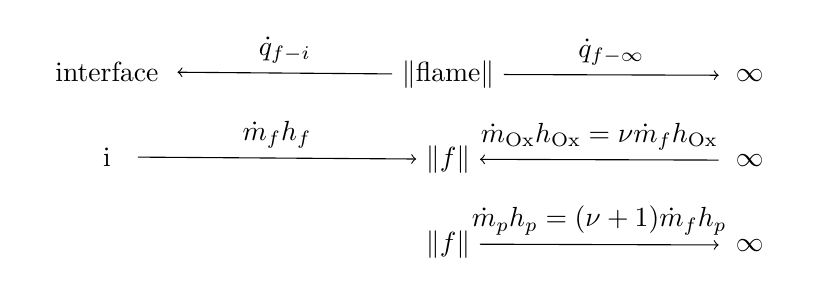
\begin{tikzpicture}
  \matrix (m) [matrix of math nodes, row sep=1.4em, column sep=7.8em, minimum width=2.2em]
  {
\text{ interface } & \| \text{flame} \| & \infty \\ 
\text{ i } & \|f \| & \infty \\ 
           & \| f \| & \infty \\ 
};
  \path[->]
  (m-1-2) edge node [above] {$ \dot{q}_{f-i} $} (m-1-1)
  (m-1-2) edge node [above] {$ \dot{q}_{f-\infty} $ } (m-1-3)
  (m-2-1) edge node [above] {$ \dot{m}_f h_f $ } (m-2-2)
  (m-2-3) edge node [above] {$ \dot{m}_{\text{Ox}}h_{\text{Ox}} = \nu \dot{m}_f h_{\text{Ox}} $ } (m-2-2)
  (m-3-2) edge node [above] {$ \dot{m}_p h_p = (\nu + 1) \dot{m}_f h_p $ } (m-3-3)
  ;
\end{tikzpicture} 
\]

Thus
\[
\begin{gathered}
  \dot{m}_f [ h_f + \nu h_{\text{Ox}} - (\nu + 1) h_f ]  = \dot{q}_{f-i} + \dot{q}_{f-\infty} \\
  \Delta h_c (T_{\text{ref}}) = h_{f,f}^{\circ} + \nu h^{\circ}_{\text{Ox},f} - (\nu +1)h_{f,f}^{\circ} \\ 
  \dot{m}_f \Delta h_c = \dot{q}_{f-i} + \dot{q}_{f-\infty}
\end{gathered}
\]
Using $\left. \frac{dT}{dr} \right|_{\text{rs}}$ from inner+outer energy conservation.  
\begin{equation}\label{Eq:DropletIV}
\boxed{   \frac{c_{pg}}{\Delta h_c} \left[ \frac{ (T_s - T_f )\exp{ (-Z_T \dot{m}_F /r_f ) } }{ \exp{ (-Z_T \dot{m}_F /r_s ) } - \exp{ (-Z_T \dot{m}_F /r_f ) } } - \frac{ (T_{\infty} - T_f )\exp{ (-Z_T \dot{m}_F /r_f ) } }{ [ 1 - \exp{ (-Z_T \dot{m}_F /r_f ) } ] } \right] - 1 = 0  }
\end{equation}

\subsection{Liquid-Vapor Equilibrium at Droplet Surface}

Clausius-Clapeyron Eqn. 
\[
p_v = p_0 \exp{ \left[ \frac{h_{fg} }{R} \left( \frac{1}{T_0 } - \frac{1}{T} \right) \right] }
\]
can rewrite as 
\[
p_v = A \exp{ \left( \frac{-B}{T_s} \right) }
\]
$A,B$ are constants for a given liquid.  

So fuel partial pressure at surface $\simeq $ equilibrium vapor.  

pressure $p_{F,s} = A\exp{ \left( \frac{-B}{T_s} \right) }$

Fuel mole fraction $X_{Fs} = \frac{p_{Fs}}{p}$ and 
\[
Y_{F,s} = \frac{N_F m_F}{ N_F m_F + N_P m_P } = X_F \frac{m_F}{ X_F m_F + (1-X_F)m_P }
\]

\begin{equation}\label{Eq:DropletV}
  \boxed{ Y_{F,s} = \frac{A \exp{ (-B/T_s) } m_F }{ A\exp{ (-B/T_s) }m_F + [p- A \exp{ (-B/T_s) }]m_P } }
\end{equation}


\subsubsection{Empirical relations}

Turns (2011) \cite{STurns2011} quotes Law and Williams (1972) (cf. Law, C.K., and Williams, F.A., ``Kinetics and Convection in the Combustion of Alkane Droplets,'' \emph{Combustion and Flame}, 19(3): 393-406 (1972)) for empirical relations to use for $k_g$ and $c_{pg}$ (EY : 20160227 I need to check this article out myself).  

Therefore, 
\begin{equation}
  \boxed{
\begin{gathered}
  c_{pg} = c_{pF}(\overline{T}) \\ 
  k_g = 0.4 k_F(\overline{T}) + 0.6 k_{\text{Ox}}(\overline{T}) \\ 
  \rho_l = \rho_l(T_s)
\end{gathered}
}
\end{equation}

Also, from 20160129 Dr. Polk, Ae121b Winter 2016, $\overline{T} = (T_s + T_f)/2$, and a good initial guess for $T_s$ and $T_f$ are $T_b(P)$ and $T_{\text{ad}}$, the adiabatic flame temperature for stoichiometric mixture.  






After algebraic manipulations (which can be done in \verb|BurningDroplet.py| with \verb|sympy| in Python, instead of by hand), then we have 5 equations
\begin{itemize}
\item \begin{equation}
  \dot{m}_F = \frac{4\pi k_g r_s }{c_{pg}} \ln{ [1 + B_{oq}]}
\end{equation}
\item \begin{equation}
  T_f = \frac{q_{i-l} + h_{fg}}{ c_{pg}(1+\nu ) } [ \nu B_{oq} - 1 ] + T_s
\end{equation}
\item \begin{equation}
  r_f = r_s \frac{ ln{ (1+B_{oq } )} }{ \ln{ [ (\nu +1)/\nu ] } }
\end{equation}
\item \begin{equation}
  Y_{F,s} = \frac{B_{oq} - 1/\nu }{ B_{oq}  +1 }
\end{equation}
\item \begin{equation}
  T_s = \frac{-B}{ \ln{ \left[ \frac{-Y_{F,s} p m_P }{ A(Y_{F,s} m_F - Y_{F,s} m_P - m_F ) } \right] } }
\end{equation}
\end{itemize}
with 
\[
B_{oq} := \frac{\Delta h_c/\nu + C_p(T_{\infty} -T_s) }{ q_{i-l} + h_{fg} }
\]

Keep in mind the constant decrease in the size of the droplet, measured by diameter squared, or $D^2$, 
\[
\frac{dD^2}{dt} = -\kappa
\]
with 
\[
\kappa := \frac{ 8 k_g}{\rho_l c_{pg}} \ln{(1+ B_{oq} ) }
\]
I will compare with Turns (2011) \cite{STurns2011}, from pp. 378, Section \textbf{Simple Model of Droplet Burning} of Chapter 10 Droplet Evaporation and Burning.  

Turns (2011) \cite{STurns2011} lists 10 assumptions on pp. 379 for the Simple Model of Droplet Burning.  Beginning with his fifth assumption,

The gas phase consists of only 3 species: fuel vapor, oxidizer, and combustion products.  The gas phase region is divided into 2 zones, inner zone, and outer zone.  So for this spherically symmetric problem, parametrize space by radius $r \in \mathbb{R}^+$ from the center of the (fuel) droplet. 

Assumption 3 of Turns (2011) \cite{STurns2011}: Fuel is single-component liquid with $0$ solubility for gases.  Phase equilibrium at liquid-vapor interface (which I believe is at the surface of the droplet, $r_s$).  

Assumption 10 of Turns (2011) \cite{STurns2011}: ``Liquid fuel droplet is the only condensed phase; no soot or liquid water is present.''

$Y_F \equiv $ fuel vapor mass fraction.  

\subsubsection{Inner zone}

Define the inner zone $r \in [r_s,r_f]$ between droplet surface $r_s$ and flame front $r_f$.  

Inner zone only contains fuel vapor and combustion products: binary diffusion prevails.

$T_s \equiv $ droplet surface temperature.   \\
$T_f \equiv $ flame temperature.   \\
$Y_{F,s} = Y_F(r=r_s) \equiv Y_F(r_s) = $ fuel vapor mass fraction at the droplet surface

$Y_F(r_f)=0$ means that all the fuel is consumed by the time we reach the flame front.  

Turns mentions that ``a more elegant approach'' is described in Kuo's \textbf{Principles of Combustion}, that ``combines the species and energy equations to create a conserved-scalar variable.  



\section{Combustion Chamber Flow Model}

cf. 20160202 Ae121b Dr. Polk.  

Parametrize the axisymmetric axis $x \in \mathbb{R}$, with $x=0$ being the inlet exit into the combustion chamber.  

Consider the (mass) inlet flow of the oxidizer, $\dot{m}_{\text{Ox}}(x=0) \equiv \dot{m}_{\text{Ox}}(0)$ and the (mass) inlet flow of the fuel $F$, $\dot{m}_{\text{F}}(x=0) \equiv \dot{m}_{\text{F}}(0)$.  Here, fuel is a vapor (i.e. gas).  

Suppose some of the fuel from the inlet will come in as a liquid $l$; denote the inlet flow of liquid fuel as $\dot{m}_l(0)$.  

\setlength{\unitlength}{1cm}
\begin{picture}(10,5.5)(-5,-2.75)
\linethickness{1pt}
\put(-3.7,0.4){{ gaseous $\{ \begin{gathered} \dot{m}_{\text{F}}(0) \\ \dot{m}_{\text{Ox}}(0) \end{gathered} \}$ }}
\put(-3.7,-0.4){{ liquid $\dot{m}_l(0)$ }}
\put(0.1,0.0){{ $$ }}
\put(-0.5,0.2){\vector(1,0){2}}
\put(-0.5,0.7){\vector(1,0){2}}
\put(-0.5,-0.3){\vector(1,0){2}}
\put(0,1.0){\line(1,0){1.5}}
\put(0,1.0){\line(0,-1){2.0}}
\put(0,-1.0){\line(1,0){1.5}}
\qbezier(1.5,1.0)(2.1,0.7)(2.3,0.6)
\qbezier(1.5,-1.0)(2.1,-0.7)(2.3,-0.6)
\put(2.3,0.6){\line(1,0){.2}}
\put(2.3,-0.6){\line(1,0){.2}}
\qbezier(2.5,0.6)(4.5,1.4)(7.5,1.8)
\qbezier(2.5,-0.6)(4.5,-1.4)(7.5,-1.8)
\put(7.5,0.0){{ $$}}
\end{picture}

Consider the following assumptions:
\begin{itemize}
\item There are only \textbf{2 phases}: the gaseous phase of fuel $+$ oxidizer, and the liquid phase of liquid fuel.
\item Assume 1-dimensional flow, with no diffusion in the bulk fluid.  
\item Assume constant pressure in the combustion chamber, and adiabatic flow, with no work on the flow.  
\item Fuel is injected as a \emph{monodisperse} spray, meaning that all the droplets have the same initial diameter.
\item Gas phase is in equilibrium at even the axial position $x$.  
\end{itemize}

The parameters of interest along the axis $x$ are the following:
\[
\begin{aligned}
  & \dot{m}_g(x) \\ 
  & T_g(x) \\
  & \phi_g(x) \\
  & v_g(x) 
\end{aligned} \quad \quad \, \begin{aligned}
  &  \dot{m}_l(x) \\
  &  D(x) \\
  & v_d(x)
\end{aligned}
\]

\subsection{Inlet conditions}

$\dot{m}_g(0)$ refers to the inlet.  \\
$\dot{m}_f(0)$ refers to flow rate of fuel injected as gas. 

Then by accounting for the total mass of the gas injected at the inlet, being part gaseous fuel, $f$, and gaseous oxidizer, Ox,
\[
\dot{m}_g(0) = \dot{m}_f(0) + \dot{m}_{\text{Ox}}(0)
\]

By definition,
\[
\left( \frac{ F}{O} \right)_x = \frac{ \dot{m}_F(x) }{ \dot{m}_{\text{Ox}}(x) }
\]
Now
\[
\phi_g(x=0) = \phi_g(0) = \frac{ \dot{m}_f(0) / \dot{m}_{\text{Ox}}(0) }{ (F/O)_{ \Phi=1} } = 0.45 
\]
by definition of an \emph{equivalence ratio}, $\phi_g$ for the gas $g$, and so we can determine $\dot{m}_f(0)$ after doing some algebra
\begin{equation}\label{Eq:dotm_f_from_phi_g}
\dot{m}_f(0) = \dot{m}_{\text{Ox}}(0) \left( \frac{F}{O} \right)_{\Phi=1} \phi_g(0)
\end{equation}

Now, if given an overall equivalence ratio, $\phi_{\text{overall}}$ at a point $x$ along the axis,
\begin{equation}\label{Eq:phi_overall}
\begin{gathered}
  \phi_{\text{overall}}(x=0) = \frac{ \dot{m}_{\text{fuel}}(0)/ \dot{m}_{\text{Ox}}(0) }{ (F/O)_{\Phi=1} } = \frac{ \frac{\dot{m}_f(0) }{ \dot{m}_{\text{Ox}}(0) } + \frac{\dot{m}_l(0) }{ \dot{m}_{\text{Ox}}(0) } }{ (F/O)_{\Phi=1} } = \phi_g(0) + \frac{ \frac{\dot{m}_l(0) }{ \dot{m}_{\text{Ox}}(0) } }{ (F/O)_{\Phi=1} }
\end{gathered}
\end{equation}
Clearly, the total mass of fuel inputted in is the mass of the fuel as a gas and mass of the fuel as a liquid (droplets):
\begin{equation}\label{Eq:dotm_totalFuel}
\dot{m}_{\text{Fuel}}(0) = \dot{m}_f(0) + \dot{m}_l(0)
\end{equation}

By the physical parameters of a given setup, such as injection velocity of the gas $v_g(x=0)\equiv v_g(0)$ and total fuel injector cross-sectional area, $A_{\text{inlet Fuel}}$ 
\begin{equation}\label{Eq:dotm_f_from_def}
% \dot{m}_f(0) = \rho_f v_f(0) A_{\text{inlet Fuel}} = \rho_f(T_{\text{inlet}},P) v_f(0) A_{\text{inlet Fuel}} 
\dot{m}_g(0) = \rho_g v_f(0) A_{\text{inlet Fuel}} = \rho_g(T_{\text{inlet}},P) v_f(0) A_{\text{inlet Fuel}} 
\end{equation}
where we remember that $\rho_f$ is a function of inlet temperature $T_{\text{inlet}}$ and pressure $P$ of the combustion chamber.  $\rho_g$ can be obtained by setting the state of the gas with \emph{Cantera}, with the appropriate equivalence ratio for the gases $\phi_g(0)$.  

From Eq. \ref{Eq:dotm_f_from_phi_g}, we can obtain $\dot{m}_{\text{Ox}}(0)$ with the help of Eq. \ref{Eq:dotm_f_from_def}, namely 
\[
\dot{m}_g(0) = \dot{m}_{\text{Ox}}(0) \left( 1 + \left( \frac{F}{O} \right)_{\Phi=1} \phi_g(0) \right)
\]  

And then, from the first equality of Eq. \ref{Eq:phi_overall}, and Eq. \ref{Eq:dotm_totalFuel}, then $\dot{m}_l(0)$ can be obtained, namely
\[
\phi_{\text{overall}}(0) (F/O)_{\Phi=1} = \frac{ \dot{m}_f(0) + \dot{m}_l(0) }{ \dot{m}_{\text{Ox}}(0) }
\]  

\subsection{Gas phase continuity}

Since for a gas, $pV=N\tau$, so \\
$p=\frac{N}{V} \tau = \frac{MN}{V} \frac{1}{M} \frac{T}{k_B}  =\rho \frac{1}{Mk_B}T = \rho R_M T$
\begin{equation}
  \boxed{ v_g = \frac{\dot{m}_g}{\rho_g A } = \frac{ \dot{m}_g R_U T_g}{ m_g PA} }
\end{equation}
i.e. $v_g = \frac{ \dot{m}_g \tau_g}{ M_g pA }$


\subsection{Gas phase Energy Conservation}

For $H_{\text{tot}} = H_{\text{tot}}(\tau,p,\lbrace N_i \rbrace , x) \equiv H_{\text{tot}}(x) \in C^{\infty}(\Sigma \times N) = C^{\infty}(\Sigma\times \mathbb{R})$, $H_{\text{tot}} = m_g h_g + m_l h_l$.  

For $\dot{H}_{\text{tot}} = \dot{m}_gh_g + \dot{m}_l h_l$ where I take into consideration the steady state assumption, then by \\
$Q =0$, $dH=0$, for $dp=0$ $\Longrightarrow \frac{d}{dx}(\dot{m}_g h_g ) + \frac{d}{dx}(\dot{m}_l h_l) =0$

Assume constant $T$ droplets, so $h_l =$ constant
\begin{equation}\label{Eq:GasPhase1dimenthalpyadiabaticflow}
\frac{dh_g}{dx} = \frac{-1}{\dot{m}_g} \left[ h_g \frac{d\dot{m}_g}{dx} + h_l \frac{d\dot{m}_l }{dx} \right]
\end{equation}
Since $h_g = h_g(T_g, p , \phi_g) \in C^{\infty}(\Sigma)$, 
\begin{equation}\label{Eq:GasPhase1dimenthalpy}
\frac{dh_g}{dx} = \frac{ \partial h_g}{ \partial T} \frac{dT}{dx} + \frac{ \partial h_g}{\partial \phi_g} \frac{d\phi_g}{dx} \qquad \, (\text{$p$ is const.})
\end{equation}
Equating Eqns. \ref{Eq:GasPhase1dimenthalpyadiabaticflow}, \ref{Eq:GasPhase1dimenthalpy}, then
\[
\frac{dT_g}{dx} = \left[ \frac{-1}{\dot{m}_g} \left( h_g \frac{d\dot{m}_g}{dx} + h_l \frac{d\dot{m}_l}{dx} \right) - \frac{ \partial h_g}{ \partial \phi_g} \frac{d\phi_g}{dx} \right]/\frac{ \partial h_g}{\partial T_g}
\]
Using mass conservation on fuel, $\frac{d\dot{m}_g}{dx} = -\frac{d\dot{m}_l}{dx}$, so
\begin{equation}
\boxed{ \frac{dT_g}{dx}= \left[ \frac{-1}{\dot{m}_g} \frac{d\dot{m}_g}{dx}(h_g - h_l) - \frac{\partial h_g}{ \partial \phi_g} \frac{d\phi_g}{dx} \right]/\frac{ \partial h_g}{ \partial T_g} }
\end{equation}



\subsection{Droplet momentum conservation}


\[
F_d = m_d \frac{dv_d}{dt} = m_d \frac{dx}{dt} \frac{dv_d}{dx} = m_d v_d \frac{dv_d}{dx}
\]
\[
\text{ $F_d$ for a sphere } = C_d \rho_g \frac{v_{\text{rel}}^2}{2} \frac{ \pi D^2}{4}
\]
Recall the Reynolds number for a sphere moving through a fluid,
\[
\text{Re} = \frac{D_{\text{droplet}} u_{\text{rel}} \rho_{\text{fluid}}}{\mu_{\text{fluid}}}
\]
where $\mu $ viscosity of the fluid, $\rho_{\text{fluid}} = \rho_g$, $\mu_{\text{fluid}} = \mu_g$.  Keep in mind that $[D_{\text{droplet}} u_{\text{rel}} \rho_{\text{fluid}}] = m\cdot \frac{m}{s} \cdot \frac{\text{kg}}{m^3} = \frac{kg}{m\cdot s}$.


\begin{equation}\label{Eq:ConvectionDropletODEs}
  \begin{aligned}
    & \frac{dD^2}{dx} = \frac{-K}{v_d} \\ 
    &  \frac{dv_d}{dx} = \frac{3C_D \rho_g (v_g-v_d)|v_g-v_d| }{ 4\rho_l Dv_d} \\ 
    & \frac{dT_g}{dx} = \left[ \frac{-1}{\dot{m}_g} \frac{d\dot{m}_g}{dx} (h_g-h_l) - \frac{\partial h_g}{\partial \phi_g} \frac{ d\phi_g}{dx} \right]/ \frac{ \partial h_g}{\partial T_g}
  \end{aligned}
\end{equation}


$\text{droplet} \in \Sigma \times \Gamma(TN)$ 

$(\rho_l,p_l) \times (x,v_d(x))$

assume constant $T$ droplets. 

So I claim by clausius Clapeyron $T_l = T_{\text{boil}}$

Let's take a look at Eq. \ref{Eq:ConvectionDropletODEs}.  

\begin{itemize}
\item Looking at $\frac{dD^2}{dx} = \frac{-K}{v_d}$, and looking at what each of the factor's respective formulae,
\[
\frac{dD^2}{dx} = \frac{-K}{v_d} \Longrightarrow \begin{gathered}
  K = \frac{ 8 k_g}{\rho_l C_{pg}} \ln{ (1+B_{oq})} \\
  B_{oq} = \frac{ \Delta h_c/\nu  + C_{pg}(T_{\infty}-T_s)  }{ q_{i-l} + h_{fg} }
\end{gathered}
\]
Then, examining the terms \emph{related to gases} that depend on $\Sigma$ and spatial manifold $N$, parametrize by $x\in \mathbb{R}$, 
\[
\begin{gathered}
  k_g = k_g(T_g,P,\phi_g) \in C^{\infty}(\Sigma) \\
  k_g(T_g(x), P, \phi_g(x)) \in C^{\infty}(\Sigma_x) \Longrightarrow k_g(x) \in C^{\infty}(N)
\end{gathered}
\]
with $\Sigma \to N$ being a fibered bundle, with fibers $\Sigma_x$.  

Likewise,
\[
\begin{gathered}
  C_{Pg} = C_{Pg}(T_g,P,\phi_g) \in C^{\infty}(\Sigma) \\ 
  C_{Pg}(T_g(x), P, \phi_g(x)) \in C^{\infty}(\Sigma_x) \text{ and } C_{Pg}(x) \in C^{\infty}(N)
\end{gathered}
\]
In $B_{oq}$, for term $h_{fg}$, for the heat of formation,
\[
\begin{gathered}
h_{fg} = h_{fg}(T^0, P, \phi_g) \in C^{\infty}(\Sigma) \\
h_{fg}(T^0,P,\phi_g(x)) \in C^{\infty}(\Sigma_x) \text{ and } h_{fg}(x) \in C^{\infty}(N)
\end{gathered}
\]
and since assuming $C_{PF} = C_{P\text{Ox}} = C_{pg}$ then
\[
\Delta h_c =\Delta h_c(T) \in C^{\infty}(\Sigma) \text{ and } \Delta h_c(T=T_{\text{ref}}) \equiv \Delta h_c(T_{\text{ref}}) = \Delta h_c(T)
\]
with the upshot that the ``heat of combustion'' is the same at $T=T_{\text{ref}}$ and at arbitrary $T$.  

For terms involving the droplet, the ``\emph{liquid}'',
\[
\begin{gathered}
  \rho_l = \rho_l(T) \in C^{\infty}(\Sigma) 
  \rho_l(T(x)) \in C^{\infty}(\Sigma_x) \text{ and } \rho_l(x) \in C^{\infty}(N)
\end{gathered}
\]
In our particular case, we assume the droplet has uniform temperature, which happens to be the temperature at the surface, which then happens to be dependent on pressure, by the Clausius-Clapeyron relation.  Keep in mind that the relation $\rho_l = \rho_l(T)$ is from the relation involving the volumnic thermal expansion $\alpha$ of a \emph{liquid}: $\rho = \frac{\rho_{T_0}}{ 1 + \alpha (T-T_0)}$, which, I think, is an empirical relation, as $\alpha$ needs to be measured and is a parameter to input in.  
\[
\rho_l = \rho_l(T_s) = \rho_l(T_b)\in C^{\infty}(\Sigma) 
\]

\item Looking at $\frac{dv_d}{dx} = \frac{3C_D \rho_g (v_g-v_d)|v_g-v_d| }{ 4\rho_l Dv_d}$, and taking a look at terms involving the \emph{gaseous} phase,
\[
\begin{gathered}
  v_g \in TN
  (x,v_g) = v_g(x) \in T_xN
\end{gathered}
\]
and 
\[
\begin{gathered}
  \rho_g = \rho_g(T_g,p,\phi_g) \in C^{\infty}(\Sigma) \\ 
  \rho_g(T_g(x),p, \phi_g(x)) \in C^{\infty}(\Sigma_x) \text{ and } \rho_g(x) \in C^{\infty}(N)
\end{gathered}
\]

Looking at terms involving the \emph{liquid} phase, the \textbf{droplet},
\[
\begin{gathered}
  v_d \in TN \\
  (x,v_d) = v_d(x) \in T_xN \\
  D=D(x) \in C^{\infty}(N)
\end{gathered}
\]

Then, examining the formulae for the Reynolds number $\text{Re}$ and $C_D$, affecting the drag on the droplet, 
\[
\begin{gathered}
  \text{Re}_{D,\text{rel}} = \frac{ D|v_g-v_d| \rho_g }{\mu}
\end{gathered}
\]
with viscosity $\mu$ being a transport property of the \emph{gas} that the droplet is moving around in, and
\[
\begin{aligned}
  & \mu = \mu(T_g,P,\phi_g) \in C^{\infty}(\Sigma) \\ 
  & \mu(T_g(x),P,\phi_g(x)) \in C^{\infty}(\Sigma_x) \text{ and } \mu(x) \in C^{\infty}(N)
\end{aligned}
\]
$C_D$ drag coefficient is fairly straightforward, depending upon $x\in N$, but through $\text{Re}_{D,\text{rel}}$, \emph{only}:
\[
C_D \simeq \frac{24}{ \text{Re}_{D,\text{rel}} } + \frac{ 6 }{ 1 + \sqrt{ \text{Re}_{D,\text{rel}} } } + 0.4
\]

\item Looking at $\frac{dT_g}{dx} = \left[ \frac{-1}{\dot{m}_g} \frac{d\dot{m}_g}{dx} (h_g-h_l) - \frac{\partial h_g}{\partial \phi_g} \frac{ d\phi_g}{dx} \right]/ \frac{ \partial h_g}{\partial T_g}$, the terms involving the \emph{gas} phase are the following:
\[
\begin{gathered}
  T_g \in \Sigma \text{ and } T_g(x) \in \Sigma(x) \equiv \Sigma_x \text{ and } \\
  T_g(x) \in C^{\infty}(N) \\
  \phi_g = \phi_g(x) \in C^{\sigma}(\Sigma_x) \text{ and } \\
  \phi_g(x) \in C^{\infty}(N) \\ 
  h_g = h_g(T_g,P,\phi_g) \in C^{\infty}(\Sigma) \\ 
  h_g(T_g(x),P,\phi_g(x)) \in C^{\infty}(\Sigma_x) \text{ and } h_g(x) \in C^{\infty}(N) 
\end{gathered}
\]
and the (physical) quantity that doesn't depend upon $\Sigma$ for the \emph{gaseous} phase is
\[
\dot{m}_g = \dot{m}_g(x) \in C^{\infty}(N)
\]

For the terms involving the droplet, or the \emph{liquid} phase,
\[
\begin{gathered}
  h_l = h_l(T_l,P) \in C^{\infty}(\Sigma) \\
  h_l(T_s,P) = h_l(T_{\text{boil}},P) \in C^{\infty}(\Sigma)
\end{gathered}
\]

\end{itemize}

\subsubsection{Considerations of the physical parameters involved}

Start with the ``mass flow'' rates that are smooth functions of space $N$.  There are \emph{2} reactant \emph{species} involved, the fuel and oxidizer, Ox, amongst \emph{2} phases, gas and liquid, considered.  
\[
\dot{m}_g = \dot{m}_g(x), \dot{m}_f = \dot{m}_f(x), \dot{m}_{\text{Ox}} = \dot{m}_{\text{Ox}}(x), \dot{m}_l = \dot{m}_l(x) \in C^{\infty}(N)
\]
Clearly, we have
\begin{equation}
\dot{m}_g = \dot{m}_f + \dot{m}_{\text{Ox}}
\end{equation}
as gaseous oxidizer is injected in, and gaseous fuel is from the evaporation off the liquid droplet.  

Modelling the liquid fuel being injected into the combustion chamber through an injection plate of total fuel injection cross-section $A_{\text{tot fuel inj}}$, at injection speed $v_d(0)$, then clearly
\begin{equation}\label{Eq:dotm_l0_def}
\dot{m}_l(x=0) = \dot{m}_l(0) = \rho_l v_d(0) A_{\text{tot fuel inj}} = \rho_l(T_b,P) v_d(0) A_{\text{tot fuel inj}}
\end{equation}
I would argue that for the liquid density $\rho_l = \rho_l(T_b,P)$, which is completely specified by 2 thermodynamic quantities in $\Sigma^l$, $(T,P) \in \Sigma^l$, the temperature is $T_b$, the boiling temperature specified by the Clausius-Clapeyron relation for a given combustion chamber pressure $P$.  The inlet temperature is usually much higher than the boiling temperature of our fuel: we wouldn't have any liquid, or droplets, if its local temperature is this inlet temperature.  I will also argue that the liquid droplet is entirely in thermal equilibrium and at its surface, fuel molecules are evaporating away at $T_b$: so the entire liquid is at $T_b = T_b(P)$.  This remains the case as the liquid droplet travels throughout the combustion chamber.

Out of this injection plate, for a droplet of initial size $D_0$, then for number of droplets per unit time emerging out of the injection plate, $\dot{\mathcal{N}}$, clearly
\[
\dot{m}_l(0) = \frac{ \dot{\mathcal{N}} \rho_l \pi D_0^3}{ 6 }
\]

Consider the so-called equivalence ratio; in this case the overall equivalence ratio $\phi_{\text{overall}}$.  It is an interesting quantity that relates purely physical quantities, masses or number of particles (i.e. moles), to thermodynamic variables $\lbrace N_i \rbrace_i \in \Sigma$, i.e. $\phi_{\text{overall}} \in C^{\infty}(\Sigma)$.  By definition of $\phi_{\text{overall}}$, 
\begin{equation}\label{Eq:def_phi_overall}
\begin{gathered}
  \phi_{\text{overall}} := \frac{ \frac{\dot{m}_f + \dot{m}_l }{ \dot{m}_{\text{Ox}} } }{ (F/O)_{\Phi =1} } = \frac{ \frac{ \dot{m}_g - \dot{m}_{\text{Ox}} + \dot{m}_l }{ \dot{m}_{\text{Ox}} } }{  (F/O)_{\Phi =1} } \Longrightarrow \dot{m}_g = \left( \phi_{\text{overall}} \left( \frac{F}{O} \right)_{\Phi =1} + 1 \right) \dot{m}_{\text{Ox}} - \dot{m}_l
\end{gathered}
\end{equation}
Also, by definition of the equivalence ratio of gaseous fuel to oxidizer (which is assumed to have completely vaporized into gas), $\phi_g \in C^{\infty}(\Sigma)$, 
\begin{equation}\label{Eq:def_phi_g}
\begin{gathered}
  \phi_g := \frac{ \frac{\dot{m}_f}{ \dot{m}_{\text{Ox}} } }{ \left( \frac{F}{O} \right)_{\Phi =1} } = \frac{ \frac{ \dot{m}_g - \dot{m}_{\text{Ox}} }{ \dot{m}_{\text{Ox}} } }{ \left( \frac{F}{O} \right)_{\Phi =1} } \Longrightarrow \dot{m}_g = \left( \left( \frac{F}{O} \right)_{\Phi =1} \phi_g + 1 \right) \dot{m}_{\text{Ox} } 
\end{gathered}
\end{equation}
By equating the expressions for $\dot{m}_g$ in Eqns. \ref{Eq:def_phi_overall}, \ref{Eq:def_phi_g}, then
\[
\dot{m}_{\text{Ox}} = \frac{ \dot{m}_l }{ \left( \phi_{\text{overall}} - \phi_g \right) \left( \frac{F}{O} \right)_{\Phi=1} }
\]
Notice that $\phi_{\text{overall}} > \phi_g \geq 0$.  

I haven't mentioned where this is all occurring.  Here is one important fact about the physical setup: 
\[
\dot{m}_{\text{Ox}}(x) = \dot{m}_{\text{Ox}}(0) \quad \, \forall \, x \in N
\]
i.e. the oxidizer is constantly being injected in and flowing uniformly through the chamber.

At $x=0$, the start of the combustion chamber, 
\begin{equation}\label{Eq:dotm_Ox0}
\dot{m}_{\text{Ox}}(0) = \frac{\dot{m}_l(0) }{ \left( \phi_{\text{overall}}(x=0) - \phi_g(x=0) \right) \left( \frac{F}{O} \right)_{\Phi=1} }
\end{equation}

Let's take stock of the quantities and its properties that we've discussed so far:
\[
\begin{aligned}
  \dot{\mathcal{N}}(x) = \dot{\mathcal{N}}(0) \qquad \forall \, x \in N & \qquad (\text{droplets don't split or breakup, and don't combine together}) \\ 
  \dot{m}_{\text{Ox}}(x) = \dot{m}_{\text{Ox}}(0) \qquad \, \forall \, x \in N & \qquad (\text{constant injection of oxidizer}) 
\end{aligned}
\]
and 
\[
\dot{m}_g(x) = \left( \left( \frac{F}{O} \right)_{\Phi =1} \phi_g(x) + 1 \right) \dot{m}_{\text{Ox} }(0) = \dot{m}_g(\phi_g(x)) \in C^{\infty}(\Sigma_x) 
\]
where we notice that $\dot{m}_g$ is a function of space $x\in N$ or a function of thermodynamic property $\phi_g(x)$.  Also note that the quantity $\left( \frac{F}{O} \right)_{\Phi=1}$, the so-called \emph{stoichiometric} ratio between the \emph{mass} of fuel to \emph{mass} of oxidizer that combines together in a reaction that goes to 100\% completion (hence ``stoichiometric''); once the chemical reaction is chosen, this quantity remains \emph{fixed} throughout $x\in N$.  

Thus, so far, we should carry forward these 3 physical quantities, that are completed determined by inlet conditions:
\[
(\dot{m}_l(0), \dot{\mathcal{N}}(0), \dot{m}_{\text{Ox}}(0) ) \in C^{\infty}(N_{x=0}) \times C^{\infty}(N_{x=0}) \times C^{\infty}(N_{x=0})
\]

For $x\in N$ (i.e. along the rest of the combustion chamber), and recalling this derivation,
\[
\begin{gathered}
  \frac{d}{dx} \dot{m}_l = \frac{d}{dx} ( \dot{\mathcal{N}} \rho_l \frac{\pi D^3}{6} ) = \frac{3}{2}\frac{\dot{m}_l(0) }{ D_0^3} D \frac{dD^2}{dx} \xrightarrow{ \frac{dD^2}{dx} = \frac{-K}{v_d} } \frac{-3}{2} \frac{\dot{m}_l(0) }{ D_0^3} D \frac{K}{v_d}
\end{gathered}
\]

\emph{Droplet evaporation off surface} is expressed as:
\[
\frac{d \dot{m}_g}{dx} = -\frac{d\dot{m}_g}{dx} \Longrightarrow \frac{d\dot{m}_g}{dx} = \frac{3}{2} \frac{\dot{m}_l(0) }{ D_0^3} D \frac{K}{v_d}
\]
and thus, taking the spatial derivative of both sides of Eq. \ref{Eq:def_phi_g}
\[
\frac{d\phi_g}{dx} = \frac{1}{ \left( \frac{F}{O} \right)_{ \Phi =1} \dot{m}_{\text{Ox}}(0) } \frac{d\dot{m}_g}{dx} = \frac{1}{ \left( \frac{F}{O} \right)_{\Phi =1} \dot{m}_{\text{Ox}}(0) } \frac{3}{2}\frac{\dot{m}_l(0) }{ D_0^3} D \frac{K}{v_d}
\]

By gas phase continuity,
\[
v_g = v_g(x) = \frac{\dot{m}_g}{\rho_g A_{cc}} = \frac{\dot{m}_g(x) R_U T_g(x) }{ MW_g P A_{cc}} = \frac{ \left( \left( \frac{F}{O} \right)_{\Phi =1} \phi_g(x) + 1 \right) \dot{m}_{\text{Ox}}(0) R_U T_g(x) }{ MW_g P A_{cc}}
\]

We can obtain $\dot{m}_l = \dot{m}_l(x)$ (i.e. as a function of $x\in N$):
\[
\dot{m}_l(x) = \frac{ \dot{\mathcal{N}} \rho_l(T_b,P) \pi D^3}{6}
\]
Notice that it is a function of $D=D(x) \in C^{\infty}(N)$.  

Now consider that 
\[
\frac{d\phi_{\text{overall}}}{dx} = \frac{ \frac{ d\dot{m}_g}{dx} - 0 + \frac{d\dot{m}_l}{dx} }{ \dot{m}_{\text{Ox}} \left( \frac{F}{O} \right)_{\Phi =1} } = 0 
\]
i.e. $\phi_{\text{overall}}$ is constant throughout the chamber!  This could be attributed to overall mass conservation, but it's explicitly shown above.

Therefore
\begin{equation}
\begin{gathered}
  \dot{m}_g(x) = \left( \phi_{\text{overall}} \left( \frac{F}{O} \right)_{\Phi=1} + 1 \right) \dot{m}_{\text{Ox}}(0) - \dot{m}_l(x) \\
  \Longrightarrow \phi_g(x) = \left( \frac{\dot{m}_g(x)}{ \dot{m}_{\text{Ox}}(0) } - 1 \right) \frac{ 1}{ \left( \frac{F}{O} \right)_{\Phi=1} }
\end{gathered}
\end{equation}
and so $\phi_g(x)$ can be obtained from this formula above, $\forall \, x \in N$.  

It may be interesting to notice that, and to take stock of what we've uncovered so far, that the dynamic quantities (dynamic in that they'll be involved in our system of ordinary differential equations (ODEs))
\[
(T_g(x), D(x),v_d(x) ) \in C^{\infty}(\Sigma^g) \times C^{\infty}(N) \times TN
\]
along with initial (inlet) conditions
\[
( \dot{m}_{\text{Ox}}(0), \dot{\mathcal{N}}, \dot{m}_l(0) ) \in C^{\infty}(N_0) \times C^{\infty}(N_0) \times C^{\infty}(N_0)
\]
completely determines, algebraically, the quantities 
\[
(\phi_g(x), \dot{m}_g(x), v_g(x) ) \in C^{\infty}(\Sigma^g) \times C^{\infty}(N) \times TN, \qquad \dot{m}_l(x) \in C^{\infty}(N)
\]
all throughout $x\in N$.

Alternatively, and even \emph{better}, keeping the assumption that $\dot{\mathcal{N}}$ is constant, we should eliminate $\dot{\mathcal{N}}$ algebraically and write only in terms of the flow rates: starting from $\dot{m}_l(0) = \rho_l(T_{\text{boil}},P)v_d(0) A_{\text{tot fuel inj}}$, Eq. \ref{Eq:dotm_l0_def}, 
\[
\dot{m}_l(0) = \frac{ \dot{\mathcal{N}} \rho_l(T_{\text{boil}}, P) \pi D_0^3}{6} \text{ or } \frac{ \dot{m}_l(0) }{ D_0^3} = \frac{ \dot{\mathcal{N}} \rho_l(T_{\text{boil}}, P ) \pi }{ 6}
\]
and thus
\[
\dot{m}_l(x) =  \dot{m}_l(0) \left( \frac{D}{D_0} \right)^3
\]
From $\dot{m}_{\text{Ox}}(0) = \frac{ \dot{m}_l(0)}{ (\phi_{\text{overall}}(0) - \phi_g(0) ) \left( \frac{F}{O} \right)_{\Phi =1} }$, Eq. \ref{Eq:dotm_Ox0}
So then
\[
\dot{m}_g(0) = (\phi_{\text{overall}}\left( \frac{F}{O} \right)_{\Phi =1} + 1 ) \dot{m}_{\text{Ox}}(0) - \dot{m}_l(0)
\]
and for $x\in N$,
\[
\dot{m}_g(x) = \dot{m}_g(0) + \dot{m}_l(0) - \dot{m}_l(x)
\]
and for $v_g$, the initial condition and general expression for $x\in N$ is 
\[
v_g(0) = \frac{\dot{m}_g(0) R_U T_g(0) }{ MW_g(\phi_g(0)) P A_{cc} } \qquad \, v_g(x) = \frac{\dot{m}_g(x) R_U T_g(x) }{ MW_g(\phi_g(x)) P A_{cc} }
\]

Taking stock of everything so far, the overall outlook is the following:
\begin{itemize}
  \item chamber parameters are fixed and given
\[
(A_{\text{tot fuel inj}}, A_{cc}, l_{cc} ) \in (\mathbb{R}^+)^3
\]
  \item inlet parameters
\[
((T_{\text{in}},P,\phi_g(0)), \phi_{\text{overall}}, v_d(0), D(0) ) \in (\Sigma_{x=0}, C^{\infty}(\Sigma_{x=0}),TN, C^{\infty}(N)) 
\]
\end{itemize}
The use of the Clausius-Clapeyron relation for the vapor pressure, and how the thermodynamic system straddles between the liquid phase and vapor (gas) phase, yields a one-to-one mapping (isomorphism): from $p = p_0 \exp{ \left( L\left( \frac{1}{T} - \frac{1}{T^o} \right) \right)}$,
\[ 
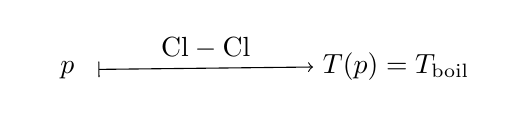
\begin{tikzpicture}
  \matrix (m) [matrix of math nodes, row sep=1.4em, column sep=7.8em, minimum width=2.2em] 
  {
p & T(p) = T_{\text{boil}} \\
};
  \path[|->]
  (m-1-1) edge node [above] {$ \text{Cl}-\text{Cl} $} (m-1-2)
  ;
\end{tikzpicture} 
\]
So for 
\[
\begin{aligned}
  & \dot{m}_l(0) = \rho_l(T_b,P)v_d(0) A_{\text{tot fuel inj}} \\ 
  & \dot{m}_{\text{Ox}}(0) = \frac{ \dot{m}_l(0) }{ (\phi_{\text{overal}} - \phi_g(0) ) \left( \frac{F}{O} \right)_{\Phi =1} } \\ 
  & \dot{m}_g(0) = \left( \phi_{\text{overall}} \left( \frac{F}{O} \right)_{\Phi =1} + 1 \right) \dot{m}_{\text{Ox}}(0) - \dot{m}_l(0) \\ 
  & v_g(0) = \frac{\dot{m}_g(0) R_U T_g(0) }{ MW_g(\phi_g(0)) PA_{cc} }
\end{aligned}
\]
and then for general $x\in N$, 
\[
\begin{aligned}
  & \dot{m}_l(x) = \dot{m}_l(0) \left( \frac{D}{D_0} \right)^3 \\ 
  & \dot{m}_g(x) = \dot{m}_g(0) + \dot{m}_l(0) - \dot{m}_l(x) \\ 
  & \phi_g(x) = \frac{ \frac{ \dot{m}_g(x) }{ \dot{m}_{\text{Ox}}(0) } - 1 }{ \left( \frac{F}{O} \right)_{\Phi =1} } \\ 
  & v_g(x) = \frac{\dot{m}_g(x) R_U T_g(x) }{ MW_g(\phi_g(x)) P A_{cc} }
\end{aligned}
\]

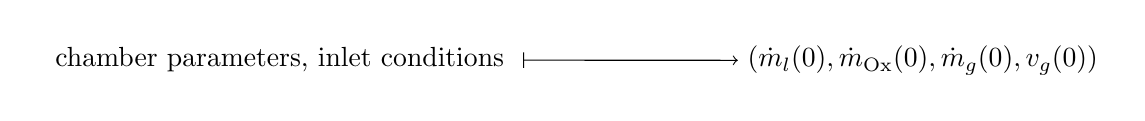
\begin{tikzpicture}
  \matrix (m) [matrix of math nodes, row sep=1.4em, column sep=7.8em, minimum width=2.2em] 
  {
\text{ chamber parameters, inlet conditions } & (\dot{m}_l(0) , \dot{m}_{\text{Ox}}(0), \dot{m}_g(0) , v_g(0)) \\
};
  \path[|->]
  (m-1-1) edge node [above] {$  $} (m-1-2)
  ;
\end{tikzpicture} 

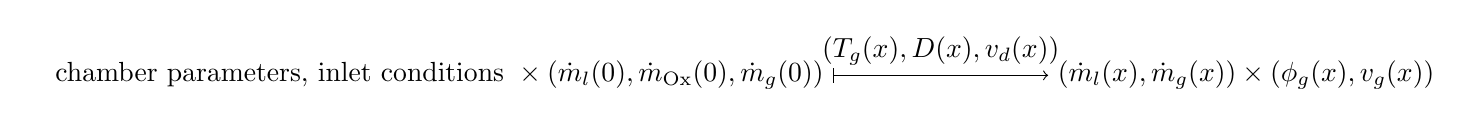
\begin{tikzpicture}
  \matrix (m) [matrix of math nodes, row sep=1.4em, column sep=7.8em, minimum width=2.2em] 
  {
\text{ chamber parameters, inlet conditions } \times (\dot{m}_l(0), \dot{m}_{\text{Ox}}(0), \dot{m}_g(0) ) & (\dot{m}_l(x) ,  \dot{m}_g(x)) \times (\phi_g(x) , v_g(x)) \\
};
  \path[|->]
  (m-1-1) edge node [above] {$(T_g(x),D(x),v_d(x))  $} (m-1-2)
  ;
\end{tikzpicture} 


\part{Numerical Computation; Scientific Computation}

\section{Interpolation and Extrapolation}

cf. Ch. 3, Interpolation and Extrapolation, Press, Teukolsky, Vetterling, Flannery (2007) \cite{PTVF2007}.

If we know $f(x)$ at $x_0, x_1, \dots x_{N-1}$, $x_0 < x_1 < \dots < x_{N-1}$,

2 interpolation processes:
\begin{enumerate}
	\item Fit (once) interpolating function to data pts. provided
	\item Evaluate (as many tiumes as you wish) that interpolating function at target pt. $x$
\end{enumerate}
Cons: typically less computationally efficient, more susceptible to round off error.

\begin{enumerate}
	\item Find right starting position in table ($x_i$ or $i$)
	\item Perform interpolation (construct functional estimate $f(x)$) using $M$ nearby values (e.g. centered on $M \ll N$ and $O(M^2)$ time (operations))
\end{enumerate}

local interpolation using $M$ nearest neighbor points gives interpolated values $f(x)$ that don't in general, have cont. 1st. or higher derivatives, \\
because, as $x= x_i$, $x=x_j$ tabulated values, interpolation scheme switches which tabulated pts. are "local" \\

where continuity of derivatives is concern, use "stiffer" interpolation by \emph{spline} function. \emph{spline} is a polynomial between each pair of table pts., but coefficients determined "slightly" nonlocally, \\
- nonlocality to guarantee global smoothness in interpolated function up to some order of derivative.

\emph{order} of the interpolation $= M - 1$, $M \equiv $ number of pts. used in interpolation scheme. \\

abscissas $x_j$, $j=0, \dots N-1$ \\
abscissas either monotonically increasing or monotonically decreasing. \\

Given $M \leq N$, number $x$, \\
find $j_{\text{lo}} \in \mathbb{Z}$ s.t. $x$ centered among $M$ abscissas $x_{j_{\text{lo}}}, \dots x_{j_{\text{lo}} }, \dots x_{j_{\text{lo}} + M - 1}$, i.e. $x\in [ x_m, x_{m+1}]$, where
\begin{equation}
	m = j_{\text{lo}} + \lfloor \frac{M-2}{2} \rfloor
\end{equation}

and $j_{\text{lo}} \nless 0$ and $ j_{\text{lo}} + M  - 1 \ngtr N - 1$ \\

If $M \mod{2} = 0$, $M = 2N$, so $ \frac{M-2}{2} = N-1$. \\
If $M \mod{2} = 1$, $M= 2N+1$, so $ \frac{M-2}{2} = \frac{2(N-1) + 1}{2} \mapsto N-1$, if $M > 2$. \\

\subsection{Polynomial Interpolation and Extrapolation}

\subsubsection{Lagrange polynomials or Lagrange's classical formula}

Given $M$ pts.
\[
\begin{gathered}
	(x_0, y_0), (x_1, y_1), \dots (x_{M - 1}, y_{M- 1})
\end{gathered}
\]
where no 2 $x_j$'s, $j= 0, 1 \dots M-1$ are equal, interpolation polynomial in Lagrange form is a linear combination:
\begin{equation}
	L(x) := \sum_{j=0}^{M- 1} y_j l_j(x)
\end{equation}
of Lagrange basis polynomials $l_j(x)$:
\begin{equation}
	l_j(x) := \prod_{ \substack{ 0 \leq m \leq M - 1 \\ m \neq j } } \frac{ x - x_m}{ x_j - x_m } = \frac{ (x- x_0) }{ (x_j - x_0) } \dots \frac{ (x- x_{j-1}) ( x - x_{j+1} ) }{ (x_j - x_{j-1} ) ( x_j - x_{j+1} ) } \dots \frac{ (x- x_{M-1}) }{ (x_j - x_{M- 1})}
\end{equation}
and so, for change of notation,
\[
\begin{gathered}
	L(x) \equiv P(x) = \frac{ (x-x_1) (x-x_2) \dots (x-x_{M-1} ) }{ (x_0 - x_1) (x_0 - x_2) \dots (x_0 - x_{M-1})} y_0 + \frac{ (x-x_0) (x-x_1) \dots (x-x_{M-2} ) }{ (x_1 - x_0) (x_1 - x_2) \dots (x_1 - x_{M-1})} y_1 + \dots + \frac{ (x-x_0) (x-x_1) \dots (x-x_{M-2} ) }{ (x_{M-1} - x_0) (x_{M-1} - x_1) \dots (x_{M-1} - x_{M-2})} y_{M - 1}
\end{gathered}
\]

For $M=2, M=3$ cases,

\[
\begin{aligned}
	& L^{(2)}(x) = \frac{ x - x_1}{x_0 - x_1} y_0 + \frac{ x- x_0 }{ x_1 - x_0} y_1 \\
	& L^{(3)}(x) = \frac{ (x - x_1)(x - x_2) }{ (x_0 - x_1) (x_0 - x_2) } y_0 + \frac{ (x - x_0)(x - x_2) }{ (x_1 - x_0) (x_1 - x_2) } y_1 + \frac{ (x- x_0)( x- x_1) }{ (x_2 - x_0)(x_2 - x_1)} y_2
\end{aligned}
\]


\section{Integration of ODEs}




\section{Systems of Ordinary Differential Equations ODEs}

EY : 20160228 There's a lack of fully general and useful examples of solving a system of ordinary differential equations (ODEs) in \verb|scipy| if one does a search on Google.  There is the \href{http://scipy-cookbook.readthedocs.org/items/numpy_scipy_ordinary_differential_equations.html}{scipy cookbook}, which has toy examples for the \href{http://scipy-cookbook.readthedocs.org/items/CoupledSpringMassSystem.html}{Coupled spring-mass system}, \href{http://scipy-cookbook.readthedocs.org/items/KdV.html}{Korteweg de Vries equation}, \href{http://scipy-cookbook.readthedocs.org/items/LoktaVolterraTutorial.html}{Matplotlib: lotka volterra tutorial}, \href{http://scipy-cookbook.readthedocs.org/items/Zombie_Apocalypse_ODEINT.html}{Modeling a Zombie Apocalypse}, \href{http://scipy-cookbook.readthedocs.org/items/Theoretical_Ecology_Hastings_and_Powell.html}{Theoretical ecology: Hastings and Powell}.  Then, there's Kevin Dunn's material for Process Model Formulation and Solution, which is \emph{excellent} for its layout, thoroughness, side-by-side comparison between Matlab and Python (scipy), and \emph{real-world} examples, though related to \emph{chemical engineering} (but which is an interesting and useful subject in its own right; so we'd might as well learn some chemical engineering).    

There was some \href{http://ocw.mit.edu/courses/chemical-engineering/10-37-chemical-and-biological-reaction-engineering-spring-2007/lecture-notes/lec05_02212007_g.pdf}{MIT OCW material on CSTR}, but it only solved for the steady-state solution.  

\subsection{Continuously Stirred Tank Reactor (CSTR)}

Consider the \emph{continuously stirred tank reactor} (CSTR) or vat or backmix reactor.  

The main assumption is of perfect mixing - perfect mixing throughout, with each locality's mixing the same as another locality, so reaction rate is equal everywhere throughout a volume $V$.  

From \href{https://en.wikipedia.org/wiki/Reaction_rate}{wikipedia's Reaction Rate} article, for a general chemical reaction of the form
\[
aA + bB \to pP + qQ
\]
the reaction rate $r$ is given by 
\[
r = \frac{-1}{a} \frac{d[A]}{dt} = - \frac{1}{b} \frac{d[B]}{dt} = \frac{1}{P} \frac{d[P]}{dt} = \frac{1}{q} \frac{d[Q]}{dt}
\]
where $[X] \equiv $ concentration of substance $X$.  

\subsubsection{Second-Order Reaction Rate}

A second order reaction rate would be of the form
\[
r = kC_A^2
\]
and if $[C_A] = \text{mol}/L$, then the units for $k$ are $[k] = \frac{ 1/s}{ \text{mol}/L} = \frac{L}{ \text{mol}\cdot s}$.  


Let's count (or account) for number of particles $N$.  In general, for concentration $n:= \frac{N}{V}$, and $N=N(t)$, dependent upon time, then
\[
\begin{gathered}
  N = \int_V n \text{vol}^n  \\
  \frac{dN}{dt} \equiv \dot{N} = \int_V \frac{ \partial n}{ \partial t} \text{vol}^n + \int_V \text{div}(nu) \text{vol}^n = \int_V \frac{ \partial n}{ \partial t} \text{vol}^n + \int_{\partial V} nu^j dS_j 
\end{gathered}
\]
One can interpretation the terms of the last equation immediately above as $[\text{accumulation}] = [\text{generation}] + ([\text{in}] - [\text{out}])$, respectively.  

Assuming perfect mixing, so the reaction rate equal everywhere throughout volume $V$, so $\frac{ \partial n}{ \partial t}$ the same throughout $V$, and that $\partial V = S_{\text{in}} \coprod S_{\text{out}}$, then
\[
\frac{dN}{dt} = \nu k C^2 V + \int_{S_{\text{in}} } nu^j dS_j + \int_{S_{\text{out}}} nu^j dS_j
\]
Now for $F(t)$ being the inlet flow of volume per second or volume per minute, then
\[
\int_{S_{\text{in}}} nu^j dS_j = F(t) C_{A,\text{in}}
\]
Supposing the flow rate out, \emph{in terms of volume}, is the same as flow rate in,
\[
\int_{S_{\text{out}} } nu^j dS_j = -F(t) C_A
\]
i.e., after perfect mixing, obtaining a concentration $n=C_A$, then multiply it by the volume per second or volume per minute flowing out, $-F(t)$ to obtain the number of particles rushing out.  

I think the flow rate out being the same as flow rate in, \emph{in terms of volume}, is what Kevin Dunn meant in the \href{http://modelling3e4.connectmv.com/wiki/Software_tutorial/Integration_of_ODEs}{first example problem for ODE integration}.  

Thus, after dividing by fixed $V$ (the volume of the tank), 
\[
\xrightarrow{ \frac{1}{V} } \frac{dn_A}{dt} \equiv \frac{dC_A}{dt} = \frac{F(t)C_{A,\text{in}}}{V} - \frac{F(t)C_A}{V} + \nu_A k C_A^2 
\]

For the ``right-hand side'' (RHS) of an ODE with constant coefficients, and a RHS that doesn't depend on time, then solving this problem is pretty easy.  In the language of flows on a manifold, letting curve, or our solution, be $\gamma :\mathbb{R} \to M$, so $\dot{\gamma} \in \mathfrak{X}(M)$, a vector field on smooth manifold $M$, then
\[
\frac{d\gamma}{dt} = f(\gamma,t) = f(\gamma) \Longrightarrow \frac{d\gamma}{f(\gamma)} = dt
\]

A copy of Dunn's implementation is in \verb|CSTRconstant.py| and \verb|CSTRdynamic.py|, copied from verbatim.  

EY : 20160229 Things I need to understand further are the \verb|set_integrator| method of \verb|scipy.integrate.ode|, with option \verb|'vode'| and method \verb|'bdf'| (i.e. \verb|method='bdf'|) and what a \href{https://en.wikipedia.org/wiki/Stiff_equation}{Stiff Equation} is. 

\section{Computational Fluid Dynamics (CFD) and Navier-Stokes equation}

Consider Liquid Bipropellant Spray Combustion Modeling (liquid bipropellant in that we are considering a liquid fuel, that's injected in, and also a liquid oxidizer, injected in), as outlined by Preclik, Knab, Estublier, and Wannerberg (Preclik, et. al.) in their article ``Simulation and Analysis of Thrust Chamber Flowfields: Storable Propellant Rockets'' (2004) \cite{YHHP2004}.  

Consider first gas-phase flow modeling.  They treat the gaseous phase in 2-dimensions, specifically in an axisymmetric coordinate axes setup, and solving, on it, the Favre-averaged Navier-Stokes equations, with species continuity, and so-called $k-\epsilon$ turbulence equations.  Let's examine first Navier-Stokes equations.

\subsection{Navier-Stokes equations}

Cuong Nguyen's notes (November 5, 2005) on \href{http://www.mit.edu/~cuongng/Site/Publication_files/TurbulenceModeling_04NOV05.pdf}{Turbulence Modeling} has an incomplete review of what RANDS is, what Favre-averaged Navier-Stokes equations is, and what $k-\omega$, $k-\epsilon$ are.    

\subsection{Spacetime $\Longleftrightarrow$ Grid}

\subsubsection{Spatial (smooth) $N$ manifold $\Longleftrightarrow$ Grid }

\[
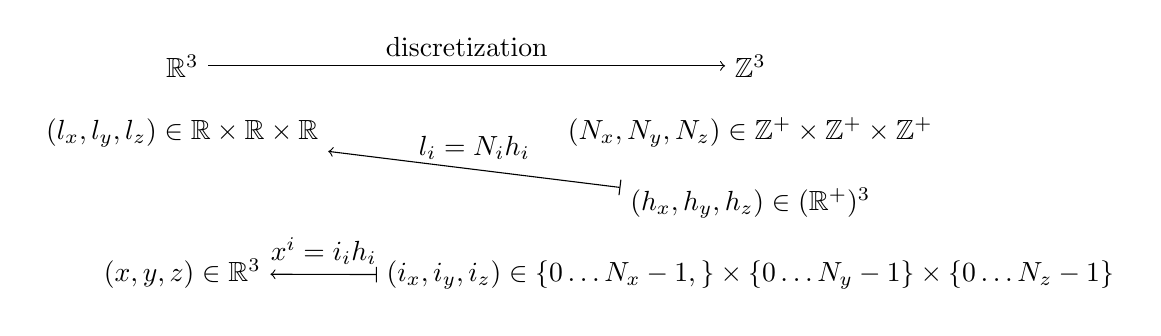
\begin{tikzpicture}
  \matrix (m) [matrix of math nodes, row sep=0.8em, column sep=1.8em, minimum width=0.6em] 
  {
    \mathbb{R}^3 & \mathbb{Z}^3 \\
    (l_x,l_y,l_z) \in \mathbb{R}\times \mathbb{R} \times \mathbb{R} & (N_x, N_y,N_z) \in \mathbb{Z}^+ \times \mathbb{Z}^+ \times \mathbb{Z}^+ \\
    & (h_x,h_y,h_z) \in (\mathbb{R}^+)^3 \\
    (x,y,z) \in \mathbb{R}^3 & (i_x,i_y,i_z) \in \lbrace 0 \dots N_x-1, \rbrace \times \lbrace 0 \dots N_y-1 \rbrace \times \lbrace 0 \dots N_z - 1\rbrace \\
    };
  \path[->]
  (m-1-1) edge node [above] {\text{discretization}} (m-1-2)
  ;
  \path[|->]
  (m-3-2) edge node [above] {$l_i = N_i h_i $} (m-2-1)
  (m-4-2) edge node [above] {$x^i = i_i h_i$ } (m-4-1)
  ;
\end{tikzpicture} 
\]

There is a \emph{flatten} functor that is necessitated by either the contiguous architecture of memory addresses on memory of the device GPU or by software constraints (CUDA C/C++ 7.5 Toolkit doesn't take multidimensional arrays).

\[
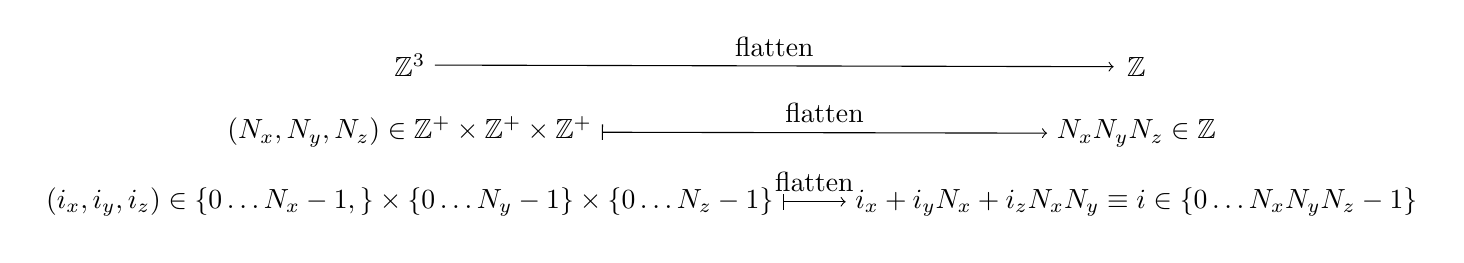
\begin{tikzpicture}
  \matrix (m) [matrix of math nodes, row sep=0.8em, column sep=2.3em, minimum width=1.6em] 
  {
     \mathbb{Z}^3 & \mathbb{Z} \\
     (N_x, N_y,N_z) \in \mathbb{Z}^+ \times \mathbb{Z}^+ \times \mathbb{Z}^+ & N_xN_y N_z \in \mathbb{Z} \\
 (i_x,i_y,i_z) \in \lbrace 0 \dots N_x-1, \rbrace \times \lbrace 0 \dots N_y-1 \rbrace \times \lbrace 0 \dots N_z - 1\rbrace & i_x + i_y N_x +i_z N_xN_y \equiv i \in \lbrace 0 \dots N_xN_yN_z-1 \rbrace \\
    };
  \path[->]
  (m-1-1) edge node [above] {\text{flatten}} (m-1-2)
  ;
  \path[|->]
  (m-2-1) edge node [above] { \text{flatten} } (m-2-2)
  (m-3-1) edge node [above] {\text{flatten} } (m-3-2)
  ;
\end{tikzpicture} 
\]
Note that $i$ is sometimes denoted as the ``global'' index in as it directly accesses the memory address on the device (GPU).  



Consider $\rho^{\infty}(\mathbb{R}^3) \in C^{\infty}(\mathbb{R}^3)$ and its behavior under the discretization (``discretize'') and flatten functors.  Also, treat $C^{\infty}(\mathbb{R}^3)$  as the ``zero''th order (trivial) vector bundle, endowed with a vector space structure itself (it's a ring, I believe, and it sits on the spatial manifold $N=\mathbb{R}^3$).  Then there is a natural projection $\pi$ back onto $N$.

\[
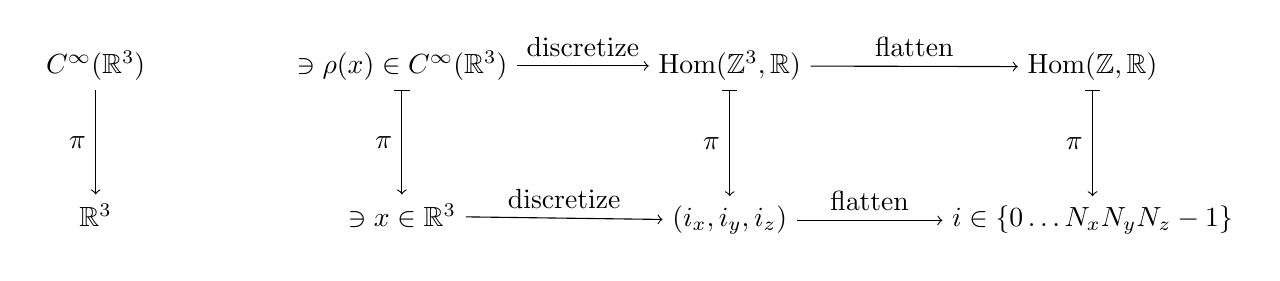
\begin{tikzpicture}
  \matrix (m) [matrix of math nodes, row sep=3.8em, column sep=4.8em, minimum width=2.9em] 
  {
   C^{\infty}(\mathbb{R}^3) & \ni \rho(x) \in C^{\infty}(\mathbb{R}^3) & \text{Hom}(\mathbb{Z}^3,\mathbb{R}) & \text{Hom}(\mathbb{Z},\mathbb{R}) \\
\mathbb{R}^3 & \ni x\in \mathbb{R}^3 & (i_x,i_y,i_z) & i \in \lbrace 0 \dots N_xN_yN_z - 1\rbrace \\
    };
  \path[->]
  (m-1-1) edge node [left] {$\pi$} (m-2-1)
  (m-1-2) edge node [above] {\text{discretize}} (m-1-3)
  (m-2-2) edge node [above] {\text{discretize}} (m-2-3)
  (m-1-3) edge node [above] {\text{flatten}} (m-1-4)
  (m-2-3) edge node [above] {\text{flatten}} (m-2-4)
  ;
  \path[|->]
  (m-1-2) edge node [left] {$\pi$} (m-2-2)
  (m-1-3) edge node [left] {$\pi$} (m-2-3)
  (m-1-4) edge node [left] {$\pi$} (m-2-4)
  ;
\end{tikzpicture} 
\]
Note that we can say that the discretization of $\rho(\mathbb{R}^3) \in C^{\infty}(\mathbb{R}^3)$ is a homomorphism $\text{Hom}$ from $\mathbb{Z}^3$ to $\mathbb{R}$ because vector space structure is preserved (and so discretization (discretize) is a functor, along with flatten).  As $C^{\infty}(N)$ is a vector space (ring) over the field $\mathbb{R}$ in that it is equipped with commutative (abelian) addition and scalar multiplication by field $\mathbb{R}$
\[
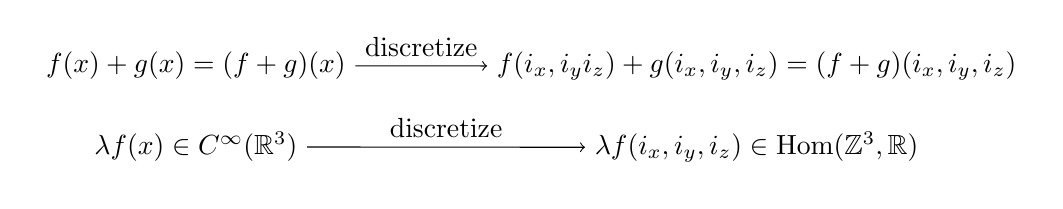
\begin{tikzpicture}
  \matrix (m) [matrix of math nodes, row sep=1.2em, column sep=4.8em, minimum width=2.9em] 
  {
    f(x) + g(x) = (f+g)(x) & f(i_x,i_yi_z) + g(i_x,i_y,i_z) = (f+g)(i_x,i_y,i_z) \\
    \lambda f(x) \in C^{\infty}(\mathbb{R}^3) &  \lambda f(i_x,i_y,i_z) \in \text{Hom}(\mathbb{Z}^3 , \mathbb{R}) \\
  };
  \path[->]
    (m-1-1) edge node [above] {\text{discretize}} (m-1-2)
  (m-2-1) edge node [above] {\text{discretize}} (m-2-2)
  ;
  \end{tikzpicture}
\]
Now consider the other object we need to consider, the vector bundle, namely the tangent bundle $TN$ over spatial (smooth) manifold $N$.  Namely consider the \emph{vector field}, representing the \emph{velocity vector field} $u$ as a section of the tangent bundle $T\mathbb{R}^3$ over Euclidean space (as a smooth manifold) $\mathbb{R}^3$.  Since $\text{dim}\mathbb{R}^3=3$, then the vector space $V \equiv T_xN$ ``over a fiber'' is of dimension 3, i.e. $\text{dim}T_xN$, $\forall \, x \in N$.
\[
u \in \mathfrak{X}(\mathbb{R}^3) = \Gamma(T\mathbb{R}^3)
\]
Recall the structure of a vector bundle, defined with a local trivialization $\varphi$ on an open set $U \subset N$:
\[
\begin{tikzpicture}
  \matrix (m) [matrix of math nodes, row sep=3.2em, column sep=4.8em, minimum width=2.9em] 
  {
TN \\
N \\
  };
  \path[->]
    (m-1-1) edge node [left] {$\pi$} (m-2-1)
  ;
  \end{tikzpicture} \qquad \, 
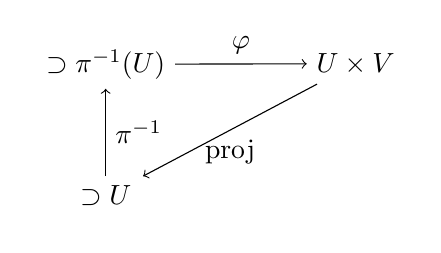
\begin{tikzpicture}
  \matrix (m) [matrix of math nodes, row sep=3.2em, column sep=4.8em, minimum width=2.9em] 
  {
\supset \pi^{-1}(U) & U\times V \\ 
\supset U & \\
  };
  \path[->]
    (m-1-1) edge node [above] {$\varphi$} (m-1-2)
  (m-2-1) edge node [right] {$\pi^{-1}$} (m-1-1)
  (m-1-2) edge node [below] {\text{proj}} (m-2-1)
  ;
  \end{tikzpicture}
\]
Then consider its behavior under discretization (discretize functor):
\[
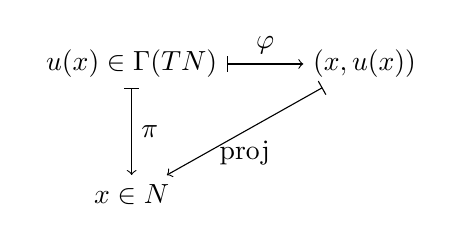
\begin{tikzpicture}
  \matrix (m) [matrix of math nodes, row sep=3.2em, column sep=2.8em, minimum width=2.4em] 
  {
u(x) \in \Gamma(TN) & (x,u(x)) \\ 
x\in N  & \\
  };
  \path[|->]
    (m-1-1) edge node [above] {$\varphi$} (m-1-2)
   edge node [right] {$\pi$} (m-2-1)
  (m-1-2) edge node [below] {\text{proj}} (m-2-1)
  ;
\end{tikzpicture} \xrightarrow{ \text{ discretize } }
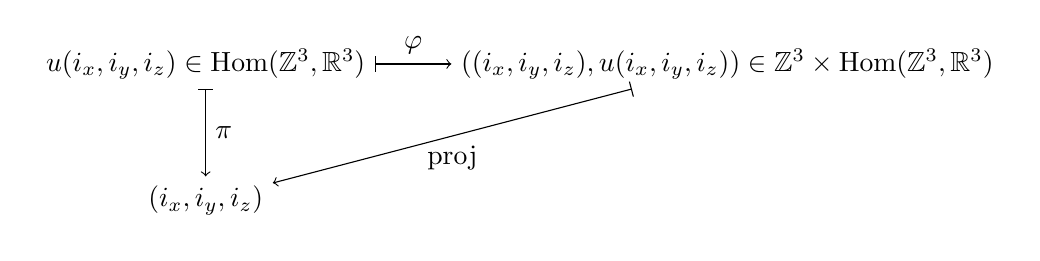
\begin{tikzpicture}
  \matrix (m) [matrix of math nodes, row sep=3.2em, column sep=2.8em, minimum width=2.4em] 
  {
u(i_x,i_y,i_z) \in \text{Hom}(\mathbb{Z}^3,\mathbb{R}^3) & ((i_x,i_y,i_z),u(i_x,i_y,i_z)) \in \mathbb{Z}^3 \times \text{Hom}(\mathbb{Z}^3 , \mathbb{R}^3) \\ 
(i_x,i_y,i_z)  & \\
  };
  \path[|->]
    (m-1-1) edge node [above] {$\varphi$} (m-1-2)
   edge node [right] {$\pi$} (m-2-1)
  (m-1-2) edge node [below] {\text{proj}} (m-2-1)
  ;
\end{tikzpicture}
\]

\subsection{Finite Volume}

\emph{Keywords:} Finite Volume, Upwind methods

Ferziger and Peric (2013) \cite{JFMP2013}.  However, here is my generalization.

\subsubsection{Upwind method}

Consider the so-called ``upwind method.''  Consider the 1-dimensional case.

Let $C_i^1 \equiv $ $i$th cell of dimension 1, for $i = 0, \dots , N-1$.  So there are $N$ total cells.

Cells are centered at $x_{2i+1} = l \frac{ (2i+1)}{2} = l(i + \frac{1}{2})$.  $l$ is the 1-dimensional size or length of a single cell.  Notice that in this case, I am assuming a uniform grid.  Note that this can be easily generalized to a grid with different cell sizes for each cell.  

For the $i$th cell, which is a 1-(cubic) simplex, a line segment, $C_i^1$, it has 2 $0$-(cubic) simplices (faces), which in this 1-dimensional case, it's 2 isolated points: $\partial C_i^1 = \lbrace C^0_{i \pm 1} \rbrace$.

The centers of these faces, i.e. the position of these 2 points, at the ends of the line segment, are
\[
x_{C^0_{i \pm 1} } = l \left( \frac{2i  +1 \pm 1 }{2} \right) = l ( i + \frac{1}{2} \pm \frac{1}{2} ) = \lbrace li, l(i+1) \rbrace
\]

I will take the mass conservation equation, in its integral form, as an example here, but this example can be easily generalized to the convection of any other conserved quantity.  Define the average mass density $\overline{\rho}_i$:
\begin{equation}
  \overline{\rho}_i := \frac{1}{l} \int_{C_i^1} \rho \text{vol}^1
\end{equation}
For the mass conservation equation (in integral form),
\begin{equation}\label{Eq:massconsvdiscretize}
\int_V  \frac{ \partial \rho}{ \partial t} = - \int_{\partial V} i_{\mathbf{u}}\rho \text{vol}^1
  \end{equation}
where the integral is taken over the volume $V$, and over its boundary $\partial V$ (which is the surface of $V$).

For the left-hand side (LHS) of Eq. \ref{Eq:massconsvdiscretize}, rewrite it in terms of $\overline{\rho}_i$,
\[
\begin{gathered}
  \int_{C_i^1} \frac{  \partial \rho}{ \partial t}(t,x) \text{vol}^1 \approx \int_{C_i^1} \frac{ \rho(t+\Delta t, x) - \rho(t,x) }{ \Delta t} \text{vol}^1 = \\
  = \frac{1}{ \Delta t} \left[ \int_{C_i^1} \rho(t+\Delta t,x) \text{vol}^1 - \int_{C_i^1} \rho(t,x) \text{vol}^1 \right] = \\
  = \frac{l}{\Delta t} \left[ \overline{\rho}_i(t+\Delta t) - \overline{\rho}_i(t) \right]
  \end{gathered}
\]

Considering the mass flux through the ``surface'' or through the endpoints of the line segment, that is a cell in the 1-dimensional case,
\[
\int_{\partial C_i^1} i_{\mathbf{u}} \rho \text{vol}^1 = \int_{ \partial C_i^1} \rho u^i dS_i
\]
then the so-called ``upwind'' scheme is this:
\[
\begin{gathered}
  \int_{C^0_{i+1}} \rho u^i dS_i = u^x(x_{C^0_{i+1}}) \int_{C^0_{i+1} } \rho dS_x = \begin{cases} 
    \overline{\rho}_iu^x(x_{C^0_{i+1}} ) & \text{ if } u^x(x_{C^0_{i+1}}) > 0 \\
    \overline{\rho}_{i+1}u^x(x_{C^0_{i+1}} ) & \text{ if } u^x(x_{C^0_{i+1}}) < 0
    \end{cases} \\
  \int_{C^0_{i-1}} \rho u^i dS_i = -u^x(x_{C^0_{i-1}}) \int_{C^0_{i-1} } \rho dS_x = \begin{cases} 
    -\overline{\rho}_{i-1}u^x(x_{C^0_{i-1}} ) & \text{ if } u^x(x_{C^0_{i-1}}) > 0 \\
    -\overline{\rho}_{i}u^x(x_{C^0_{i-1}} ) & \text{ if } u^x(x_{C^0_{i-1}}) < 0
    \end{cases} 
\end{gathered}
\]


For the 3-dimensional case, I refer back to my notes on \href{https://github.com/ernestyalumni/CompPhys/blob/master/LaTeXandpdfs/CompPhys.pdf}{Computational Physics} in the 3-dim. ``Upwind'' subsection. 


For a rectangular prism (cubic),

for cell $C^3_{ijk}$, $i=0 \dots N_x-1$, $j=0 \dots N_y-1$ , $k=0 \dots N_z-1$, $N_x\cdot N_y \cdot N_z$ total cells.

Cells centered at
\[
(x_{2i+1}, y_{2j+1}, z_{2j+1}) = (l^x \frac{ (2i+1)}{2} , l^y \frac{(2j+1)}{2}, l^z \frac{(2k+1)}{2} ) = \left( \sum_{l=0}^{i-1} l_l^x + \frac{l_i^x}{2} , \sum_{l=0}^{j-1}l_l^y + \frac{l_j^y}{2}, \sum_{l=0}^{k-1}l_l^z + \frac{l_k^y}{2}  \right)
\]
For the 3-(cubic) simplex, $C^3_{ijk}$, it has 6 2-(cubic) simplices (faces).  So for $C_{ijk}^3$, consider $\lbrace C^2_{i\pm 1, jk}, C^2_{ij\pm 1,k}, C^2_{ijk\pm 1}\rbrace$.

The center of these faces, such as for $C^2_{i\pm 1, jk}$, $x_{ C^2_{i\pm 1, jk} }$, for instance,
\[
\begin{aligned}
 x_{C^2_{i\pm 1,jk}} = (x_{2i+1\pm 1},y_{2j+1},z_{2k+1}) = (l^x\left( \frac{2i+1\pm 1}{2}\right) , l^y\frac{(2j+1)}{2},  l^z\frac{(2j+1)}{2} ) = \left( \sum_{l=0}^{ \frac{2i - 1 \pm 1 }{2} } l_l^x, \sum_{l=0}^{j-1} l_l^y + \frac{l_j^y}{2}, \sum_{l=0}^{l-1} l_l^z + \frac{l_k^z}{2} \right) 
  \end{aligned}
\]

We want the flux.  So for
\[
\overline{\rho}_{ijk} := \frac{1}{l_i^x l_j^yl^z_k} \int_{C^3_{ijk}} \rho \text{vol}^3
\]
then the flux through 2-(cubic) simplices (faces), $\int \rho i_{\mathbf{u}}\text{vol}^3$,
\[
\begin{aligned}
 &  \int_{C^2_{i+1,jk}} \rho i_{\mathbf{u}} \text{vol}^3 = \begin{cases} l_j^yl_k^z \overline{\rho}_{ijk} u^x(x_{C^2_{i+1, jk} } ) & \text{ if } u^x(x_{C^2_{i+1,jk} }) > 0 \\ 
 l_j^y l^z_k \overline{\rho}_{i+1,jk} u^x(x_{C^2_{i+1, jk} } ) & \text{ if } u^x(x_{C^2_{i+1,jk} }) < 0 \end{cases} \\
\end{aligned}
\]
\[
\begin{gathered}
  \int_{C^2_{i-1,jk}} \rho i_{\mathbf{u}} \text{vol}^3 = \int_{C^2_{i-1,jk}} \rho u^i dS_i = \int_{C^2_{i-1,jk}} \rho u^i \frac{ \sqrt{g}}{ (3-1)!} \epsilon_{ii_2i_3} dx^{i_2} \wedge dx^{i_3} = -u^x(x_{C^2_{i-1,jk}}) \int_{C^2_{i-1,jk} } \rho dy dz = \\
  = \begin{cases}
    -l_j^y l^z_k \overline{\rho}_{i-1,jk} u^x(x_{C^2_{i-1,jk}}) & \text{ if } u^x(x_{C^2_{i-1,jk}}) > 0 \\
        -l_j^y l^z_k \overline{\rho}_{i,jk} u^x(x_{C^2_{i-1,jk}}) & \text{ if } u^x(x_{C^2_{i-1,jk}}) < 0 
    \end{cases}
\end{gathered}
\]

and so on.




\subsection{Finite Difference}

Consider mass conservation.

\[
\begin{gathered}
\frac{d}{dt} M  = \frac{d}{dt} \int_V m \equiv \frac{d}{dt} \int \rho \text{vol}^d = \int \mathcal{L}_{ \frac{ \partial }{ \partial t} + \mathbf{u} } \rho \text{vol}^d = \int \frac{ \partial \rho }{ \partial t} \text{vol}^d + \mathbf{d}u_{\mathbf{u}}\rho \text{vol}^d = \int \left( \frac{ \partial \rho}{ \partial t} + \text{div}(\rho \mathbf{u} ) \right) \text{vol}^d = 0 
\end{gathered}
\]

From here,
\[
\begin{gathered}
  \frac{ \partial \rho }{ \partial t} + \text{div}(\rho \mathbf{u}) = \frac{ \partial \rho }{ \partial t} + \frac{1}{\sqrt{g}} \frac{ \partial }{ \partial x^k} (\rho u^k \sqrt{g}) = \frac{ \partial \rho}{ \partial t} + \rho \text{div}\mathbf{u} + u^k \frac{ \partial \rho }{ \partial x^k} = 0
  \end{gathered}
\]
If $\text{div}\mathbf{u} = 0$, this is the \emph{incompressible} case.

If $\sqrt{g}=1$, $\frac{ \partial \rho}{ \partial t} + \frac{ \partial }{ \partial x^k}(\rho u^k) = 0 $

\subsubsection{ 2 and more species, mass conservation}

Suppose $M_{\text{tot}} = M_A + M_B$, $\begin{aligned} \rho_{A} & = \frac{ M_A}{ | \int \text{vol}^d| } \\ \rho_{B} & = \frac{ M_B}{ | \int \text{vol}^d| } \end{aligned}$.  (assume, cf. Landau and Lifshitz, that species $A,B$ ``don't talk to each other'', that is, interaction between them is negligible in terms of occupying volume; this is what gases do).

\[
\begin{gathered}
  \dot{M}_{\text{tot}} \equiv \frac{d}{dt} M_{\text{tot}} = \frac{d}{dt}(M_A + M_B) = \frac{d}{dt} \left( \int \rho_A \text{vol}^d + \int \rho_B \text{vol}^d\right) = \frac{d}{dt} \left( \int (\rho_A + \rho_B) \text{vol}^d\right) = \\
  = \int \left( \frac{ \partial \rho_A}{ \partial t} + \text{div}(\rho_A \mathbf{u}) + \frac{ \partial \rho_B}{\partial t} + \text{div}(\rho_B \mathbf{u}) \right) \text{vol}^d   = \int \frac{ \partial (\rho_A + \rho_B) }{ \partial t} + \text{div}((\rho_A + \rho_B)\mathbf{u} ) = 0 
  \end{gathered}
\]
\begin{equation}
  \begin{gathered}
    U = U(\sigma, V,N) \\ 
    dU  = \tau d\sigma - p dV + \mu dN
    \end{gathered}
  \end{equation}


\begin{equation}
\begin{gathered}
  H=H(\sigma,p,N) := U + pV \\
dH = dU + pdV + Vdp = \tau d\sigma + \mu dN + Vdp
\end{gathered}
\end{equation}

\begin{equation}
\begin{gathered}
  G = G(\tau, p , N) = U + pV - \tau \sigma = H-\tau \sigma = \mu N \\ 
  dG = dU + pdV + Vdp - \tau d\sigma - \sigma d\tau = \tau d\sigma - pdV + \mu dN + pdV + Vdp - \tau d\sigma - \sigma d\tau = \\
  = -\sigma d\tau + Vdp + \mu dN = \mu dN + N d\mu
  \end{gathered}
  \end{equation}

\subsection{Compressible, inviscid (no viscosity) flow i.e. Euler equations}

Consider the total momentum of a fluid element $V$, $V \subset N$, $\mathbf{P}$:
\begin{equation}
  \mathbf{P} = \int_V \mathbf{p} \text{vol}^d = \int_V p^i \text{vol}^d \otimes \mathbf{e}_i
\end{equation}
where $\text{vol}^d$ is the volume $d$-form on the \emph{spatial} (smooth) manifold $N$, $N$ is of dimension $\text{dim}N = d$, $\mathbf{e}_i$ is an orthonormal basis vector of the orthonormal frame on $N$, and where $i=1,2, \dots , d$, with repeated indices imply summation (i.e. Einstein's summation notation).  $\mathbf{p} = \mathbf{p}(t,\mathbf{x})$ is a time-dependent vector field taking values on the tangent bundle of $N$, $TN$.  Note that $\mathbf{P}$ is also a time-dependent vector field, after integration of $\mathbf{p}\text{vol}^d$ over $V$: strictly speaking, one could say that $\mathbf{p}$ and $\mathbf{P}$ belongs to the space of all vector fields over $\mathbb{R}\times N$, with $\mathbf{R}$ representing time, $\mathfrak{X}(\mathbb{R}\times N) = T(\mathbb{R}\times N)$, but with the component in the time direction being strictly zero.  

Consider the (total) time derivative of $\mathbf{P}$:
\begin{equation}\label{Eq:TimeDevPEulerEqn}
  \begin{gathered}
    \dot{\mathbf{P}} \equiv \frac{d}{dt} \mathbf{P} = \frac{d}{dt} \int_V p^i \text{vol}^d\otimes \mathbf{e}_i = \int_V \left( \frac{ \partial p^i}{ \partial t} + \text{div}(p^i \mathbf{u}) \right)\text{vol}^d \otimes \mathbf{e}_i = \\
    = \int_V T^{ij} dS_j \otimes \mathbf{e}_i = -\int_V (\text{grad}p) \text{vol}^d
    \end{gathered}
  \end{equation}
where the usual ``right-hand side'' (RHS) for the Euler equations for inviscid flow is the second line of Eq. \ref{Eq:TimeDevPEulerEqn}, and there, $p$ is the pressure for the thermodynamic system at $V$.  This thermodynamic system is the (single) gas phase inside $V$.  Take $V$ small enough such that the system equilibrates \emph{locally} and thus the pressure $p$ is a good parameter to specify the thermodynamic state of the system at local equilibrium in $V$.  $p$ takes on double duty as a $C^{\infty}$ function on $\mathbb{R}\times N$, i.e. $p \in C^{\infty}(\mathbb{R}\times N)$, with $C^{\infty}(\mathbb{R}\times N)$ denoting the space of all smooth (i.e. infinitely differentiable) functions over (i.e. depending upon) $\mathbb{R}\times N$.

One thing to note about the derivation of the usual ``left-hand side'' (LHS) for the Navier-Stokes equations, as shown in the first line of Eq. \ref{Eq:TimeDevPEulerEqn}, is that the Lie derivative is only acting on the ``differential form'' part of the integrand $\mathbf{p} \text{vol}^d = p^i \text{vol}^d \otimes \mathbf{e}_i$.  This could be made clearer in considering the definition of a time derivative as a limit, and the flow of a differential form under the ``full'' velocity vector field $\frac{d}{dt} = \frac{ \partial}{ \partial t} + \mathbf{u}$, $\varphi_{\Delta t}$, where $\mathbf{u} \in \mathfrak{X}(\mathbb{R}\times N) = T(\mathbb{R}\times N)$ is the usual time-dependent velocity vector field, taking only values in $TN$.  Indeed
\begin{equation}\label{Eq:LHSderivationNavierStokes}
\begin{gathered}
  \frac{d}{dt} \int_V p^i \text{vol}^d \otimes \mathbf{e}_i := \lim_{\Delta t \to 0 } \frac{ \int_{\varphi_{\Delta t}V} p^i(t+\Delta t,\mathbf{x}) \text{vol}^d \otimes \mathbf{e}_i - \int_V p^i(t,\mathbf{x})\text{vol}^d \otimes \mathbf{e}_i }{ \Delta t} = \\
   = \lim_{\Delta t \to 0} \lbrace \int_{V} \varphi_{\Delta t}^*(p^i(t+\Delta t, \mathbf{x}) \text{vol}^d) \otimes \mathbf{e}_i - \int_Vp^i(t,\mathbf{x})\text{vol}^d \otimes \mathbf{e}_i \rbrace \frac{1}{\Delta t} = \\
   = \int_V \lim_{\Delta t \to 0} \left[ \varphi^*_{\Delta t} (p^i(t+\Delta t,\mathbf{x}) - p^i(t,\mathbf{x}) )\right]\frac{1}{\Delta t} \otimes \mathbf{e}_i =  \\
   = \int_V \mathcal{L}_{\frac{ \partial }{\partial t} + \mathbf{u}}(p^i(t,\mathbf{x}) \text{vol}^d) \otimes \mathbf{e}_i
  \end{gathered}
\end{equation}
Note that the derivation in Eq. \ref{Eq:LHSderivationNavierStokes} resolves the (possible) pitfall of perhaps taking the Lie derivative $\mathcal{L}_{\frac{\partial }{ \partial t} + \mathbf{u}}$ over the \emph{entire} integrand, $\mathbf{p}\text{vol}^d \in \Omega^d(N,TN)$, with $\Omega^d(N,TN)$ denoting the space of all $TN$-valued $d$-forms.  If that was the case, taking $\mathcal{L}_{\frac{\partial}{\partial t} + \mathbf{u}}$ over the entire integrand, we'd expect the Lie derivative to act as a ``symmetric'' derivation over a symmetric tensor product, i.e. $\mathcal{L}_{ \frac{ \partial }{ \partial t} + \mathbf{u} }( \mathbf{p} \text{vol}^d ) = (\mathcal{L}_{\frac{ \partial }{ \partial t} + \mathbf{u} }(\mathbf{p})) \text{vol}^d + \mathbf{p} \otimes (\mathcal{L}_{\frac{ \partial }{ \partial t} + \mathbf{u} } \text{vol}^d )$.  However, the derivation in Eq. \ref{Eq:LHSderivationNavierStokes} shows that this is not the case.  

The point is, or the take away is, that the total time derivative $\frac{d}{dt}$ can be ``moved into'' the integral of a vector-valued differential form and ``inside the integral,'' the Lie derivative is performed.  

We should take care of how mass density is defined in a small volume $V$.  Clearly, to obtain the total mass $M$ inside a volume $V$, we integrate over the mass density $\rho$, over $V$:
\begin{equation}
  M = \int_V \rho \text{vol}^d
  \end{equation}
Clearly, when $\rho=0$, then $M=0$, with the physical interpretation, clearly, being that there's no gas inside $V$.

Taking the total time derivative of $M$:
\begin{equation}\label{Eq:totaltimederMderivation}
\begin{gathered}
  \dot{M} = \frac{d}{dt} \int_V \rho \text{vol}^d = \int_V \frac{ \partial \rho }{ \partial t} \text{vol}^d + \int_V \mathbf{d}i_{\mathbf{u} } \text{vol}^d = \int_V \frac{ \partial \rho }{ \partial t} \text{vol}^d + \int_{\partial V} i_{\mathbf{u}}\rho \text{vol}^d = \\
  = \int_V \left( \frac{ \partial \rho }{ \partial t} + \text{div}(\rho \mathbf{u} ) \right) \text{vol}^d
  \end{gathered}
  \end{equation}
In the first line of Eq. \ref{Eq:totaltimederMderivation}, the last term, $\int_{\partial V} i_{\mathbf{u}}\rho \text{vol}^d$ expresses the mass flux through the surface of volume $V$, $\partial V$, and then, applying Stoke's law, leads to the second line of Eq. \ref{Eq:totaltimederMderivation}, leading to the divergence of $\rho \mathbf{u}$.  Multiplying vector fields by $C^{\infty}$ functions, in this case $\mathbf{u}$ and $\rho$, respectively, is ok since the space of vector fields $\mathfrak{X}(\mathbb{R}\times N)$ is a module over the commutative algebra of $C^{\infty}(\mathbb{R}\times N)$.

Mass conservation dictates that
\begin{equation}
  \dot{M} = 0 
  \end{equation}
This statement can be adapted to multiple number of species.

If $V$ can be made arbitrary and sufficiently small, then the usual statement, in differential form, of mass conservation is obtained:
\begin{equation}\label{Eq:massconsvdiff}
\frac{ \partial \rho}{\partial t} + \text{div}(\rho \mathbf{u} ) = 0 \text{ or } \frac{ \partial \rho }{ \partial t} = -\text{div}(\rho \mathbf{u} )
\end{equation}

Now, one should take special care in defining the ``momentum density'', the momentum per unit volume, $\mathbf{p}$,  with respect to the mass density, given a velocity vector field $\mathbf{u}$:
\begin{equation}
\mathbf{p} = \rho \mathbf{u}  \text{ or } p^i = \rho u^i \qquad \, i = 1, \dots , d
  \end{equation}
If $\rho =0$, then $\mathbf{p}=0$.  But it can be that $\mathbf{u} \neq 0$, say, at a particular point in $(t,\mathbf{x})$.  Then $\frac{\mathbf{p}}{\rho}$ is ill-defined.

If $\mathbf{u}=0$, but $\rho >0$, then the physical interpretation is clear: the gas is at rest.  $\mathbf{p}=0$ is thus clear.  Then $\frac{p}{\rho}$ is well-defined and so is $\mathbf{u}$ at that point $(t,\mathbf{x})$.

So Eq. \ref{Eq:massconsvdiff} gives a direct recipe for the use of finite difference methods in the next time step $t+\Delta t$, where $\Delta t$ is infinitesimally small, for $\rho$, $\rho(t+\Delta,\mathbf{x})$.  But the important point is that we may not be able to define what $\mathbf{u}$ will be in the next time step.

From Eqns. \ref{Eq:TimeDevPEulerEqn}, \ref{Eq:LHSderivationNavierStokes}, we obtain a direct recipe for the use of finite difference methods in the next time step $t+\Delta t$ for $\mathbf{p}$ or $p^i$, $i=1\dots d$:
\begin{equation}\label{Eq:momentumdiff}
\begin{gathered}
  \frac{ \partial p^i }{ \partial t} + \text{div}(p^i \mathbf{u}) = -(\text{grad}p)^i \text{ or } \frac{ \partial p^i}{ \partial t} = - \text{div}(p^i \mathbf{u}) - (\text{grad}p)^i
  \end{gathered}
  \end{equation}
As a notation note, $p$, that isn't decorated by superscript $i$'s or isn't boldfaced, refers to the \emph{pressure}, indeed the ``local'' pressure at point $(t,\mathbf{x})$; $p^i$ or $\mathbf{p}$ refer to the momentum density.

So from Eq. \ref{Eq:momentumdiff}, we obtain $\mathbf{p}(t+\Delta t, \mathbf{x})$, but we don't obtain $\mathbf{u}$ directly.  If $\rho >0$ (and the fact that $\rho$ is non-negative is a \emph{physical} fact that must be enforced in the math), then dividing $\mathbf{p}$ by $\rho$ yields $\mathbf{u}$:
\begin{equation}\label{Eq:fromprhoobtainu}
\frac{\mathbf{p}}{\rho} = \mathbf{u} \qquad \, \text{ if } \rho >0
\end{equation}
However, if $\rho =0$, then $\mathbf{u}$ is undetermined.  

My concerns are the following: in the implementation of finite difference methods, what is ``small enough'' for $\rho$ to warrant it to be effectively zero?  In Eq. \ref{Eq:fromprhoobtainu}, suppose $\rho$ is very small, but due to the floating point representation of numbers by the computer away from $0$, then $\mathbf{u}$ could be very large, perhaps ``overflowing'' the floating pointer presentation of the number.

On one level, I would think that we can check if $\rho$ is equal to $0$ or not and then if not, calculate the new $\mathbf{u}(t+\Delta t, \mathbf{x})$.  If $\rho$ is equal to $0$, then $\mathbf{u}$ is left alone.  

\subsection{Energy density}

Consider a thermodynamic system at rest.  Indeed, consider moving into the reference frame where the fluid element is at rest inside the volume $V$; this can be done at any instant $t$.

The enthalpy $H$ of this system is defined as
\begin{equation}
H := U + pV
  \end{equation}
with $U$ denoting the \emph{internal energy} of the thermodynamic system.  $U$ includes all the energy locked up in rotational and vibrational modes, chemical potential, random thermal kinetic energy, but \emph{not} the kinetic energy due to the \emph{bulk} fluid motion due to velocity vector field $\mathbf{u}$.

$H$ is a function of entropy (entropy that's \emph{not} multiplied by the Boltzmann constant; it is dimensionless in this notation) $\sigma$ of the system, pressure $p$, and the number of molecules of the species; and if there's only one species present, this is denoted as $N$; otherwise, for each species $i$, $H$ is a function of $\lbrace N_i\rbrace_i$, the number of each species present:
\[
H = H(\sigma,p,N) \text{ or } H = H(\sigma, p , \lbrace N_i \rbrace_i )
\]
In fact, the parameters $\sigma,p,\lbrace N_i \rbrace_i$ or $(\sigma,p,N)$ in the single-species case, define exactly (i.e. that's all you need to know) the state of the thermodynamic system at a given time and place $(t,\mathbf{x})$ - let these parameters be global coordinates for a manifold $\Sigma$ that represents all possible thermodynamic states of the system.

$U$ is a function of $\sigma,V,N$ or $\sigma, V,\lbrace N_i \rbrace_i$ in the multi-species case, which also specify completely the thermodynamic state of the system
\[
U = U(\sigma,V,N)
\]
Going from $U$ to $H$ is a Legendre transformation on $\Sigma$ - $\Sigma$ stays the same, but the (global) coordinates are transformed.

Nevertheless, when there is no gas in $V$, i.e. $N=0$, then define the zero $U=0$ for $N=0$.
\[
U=U(\sigma,V,0) = U(0,V,0) = 0 
\]
Notice that $\sigma=0$ in the above expression.  The physical argument is this: if there is no gas in the box of volume $V$, there is only 1 way to arrange the microstates of the thermodynamic system in such a manner, and so the $\log$ of $1$ is $0$ and so $\sigma =0$.

For $H$, we have to define what it means for $H$ to be zero carefully.  If $N=0$, then $U=0$ and so
\[
H(\sigma,p,0)= U(\sigma,V,0) + pV = 0 + pV
\]
I will argue that $p=0$ if $N=0$.  For if $N=0$, then there's no pressure to push back against the target gas system.  This is clearly the case of a vacuum.  For the case where there's already an ambient or background gas phase in and around $V$, this is also the case as well as we're concerned with the target gas system.  The background gas can be pushing against itself and have a pressure inside and around $V$, or even a pressure gradient, but if there's no target gas there at $V$, then there's nothing for this background gas to push against, other than itself.

So $H=0$ when $N=0$.

Define the (internal) energy density in this reference frame (denoted with $'$) where the fluid is at rest, the (internal) energy per unit volume, $\epsilon'$ to be
\begin{equation}
  \epsilon' := \frac{U}{V}
  \end{equation}
Define the enthalpy per unit volume $h'$ to be
\begin{equation}
  h':= \frac{H}{V} = \epsilon' + p
\end{equation}
If $\epsilon'=0$, and yet temperature of the thermodynamic system $\tau$ is positive, i.e. $\tau  >0$, then no gas is there.  Thus, also $h'=0$ as $p=0$ as argued above.

As a notation note, $\tau$ denotes the temperature in units of \emph{energy} such as joules $(J)$ or $(\text{ergs})$: use Boltzmann's constant $k_B$ as a units conversion factor between $\tau$ and the usual temperature $T$ in Kelvin
\[
\tau = k_b T
\]

Why I've elaborated upon when $U=0$ and $H=0$ and thus when $\epsilon'=0$ and $h'=0$ is because, first, the energy scale ``zero'' can be arbitrarily set and so it's good to set it once and for all, with physically meaningful reasons.  Second, there can be confusion that arises in the consideration of what it means for $H=0$ as when it is defined as $H:=U+pV$, and of what pressure $p$ refers to: the pressure that the target gas system encounters, only, or would it include the ``ambient'' pressure even if there's no gas in the local volume $V$ we're considering.  Third, these considerations stem from the concern of what it means to, in a volume $V$ with no gas initially present, put 1 molecule of gas into the fixed volume $V$ and the resulting changes in thermodynamic quantities; for instance, where there was no gas before, putting in 1 gas molecule results immediately in $pV$ work that needs to be done to restore the volume back to its initial ``fixed'' volume $V$ (see Le Bellac, Mortessagne, Batrouni (2004) \cite{MLeBellacFMortessagneGBatrouni2004} and its lucid distinguishing between \emph{convection} and \emph{conduction} for a thermodynamic system).

Clearly, when switching, i.e. ``boosting'' into the reference frame where the fluid is moving, i.e. the observer's or laboratory's frame of reference, $\epsilon'$ transforms into $\epsilon$, the (internal) energy density in this lab frame, in the following manner:
\begin{equation}
\epsilon = \epsilon' + \frac{1}{2} \rho u^2
  \end{equation}
Denote this kinetic energy density $\frac{1}{2} \rho u^2$ as $k \equiv \frac{1}{2} \rho u^2$.


For total energy in a volume $V$, $E$, given by
\begin{equation}
  E := \int_V \epsilon \text{vol}^d
  \end{equation}
then the total time derivative of $E$, $\dot{E} \equiv \frac{dE}{dt}$ is given by, from differential geometry as above,
\begin{equation}\label{Eq:dotEbalanceeqLHS}
\begin{gathered}
  \dot{E} \equiv \frac{d}{dt} \int_V \epsilon \text{vol}^d = \int \left( \frac{ \partial \epsilon }{ \partial t} + \text{div}(\epsilon \mathbf{u} ) \right) \text{vol}^d = \\
   = \int \left( \frac{ \partial \epsilon }{ \partial t} + \text{div}(k+\epsilon')\mathbf{u} \right) \text{vol}^d = \int \left( \frac{ \partial \epsilon}{ \partial t} + \text{div}(k\mathbf{u}) + \text{div}((h'-p) \mathbf{u} ) \right) \text{vol}^d = \int_V \left( \frac{ \partial \epsilon}{ \partial t} + \text{div}(k\mathbf{u}) + \text{div}(h'\mathbf{u} ) - \text{div}(p\mathbf{u}) \right) \text{vol}^d
\end{gathered}
\end{equation}
From physics, the total time derivative of the energy $E$, $\dot{E}$ is equal to the work done on the fluid system inside and about $V$ by external forces.  Neglecting body forces, the only external forces are due to stresses and strains at the surface of $V$, which are wrapped up in the stress-strain tensor $T^{ij}$.  Using Stoke's equation again, a surface integral involving $T^{ij}$ can be transformed into a volume integral.  For the case of the perfect fluid, $T^{ij}$ takes the form of $T^{ij} = g^{ij}(-p)$, where $g^{ij}$ is the metric of the spatial manifold $N$.  Thus
\begin{equation}\label{Eq:dotEbalanceeqRHS}
\begin{gathered}
  \dot{E} = \int_V \text{div}(u_iT^{ij}) \text{vol}^d = \int_V \text{div}(u_i g^{ij}(-p)) \text{vol}^d = -\int_V \text{div}(\mathbf{u}p) \text{vol}^d
  \end{gathered}
\end{equation}

Recognizing that we can subtract from both sides the $-\int_V \text{div}(\mathbf{u}p)\text{vol}^d$ term of the ``left-hand side'' and ``right-hand side'' of the ``energy balance'' equation for $\dot{E}$, Eqns. \ref{Eq:dotEbalanceeqLHS}, \ref{Eq:dotEbalanceeqRHS}, respectively, then we obtain the desired integral and differential form for the energy density $\epsilon$ under compressible fluid flow:
\begin{equation}
\begin{gathered}
  \Longrightarrow \int_V \left( \frac{ \partial \epsilon}{ \partial t} + \text{div}((k+h')\mathbf{u}) \right) \text{vol}^d =0 \Longrightarrow \boxed{ \frac{ \partial \epsilon}{ \partial t} + \text{div}((k+h')\mathbf{u}) = 0 }
  \end{gathered}
\end{equation}
Now if we can express $h'$ in terms of $\rho$ and $\mathbf{u}$, given the concerns above, and $\epsilon$, then we'd have succeeded in a complete or ``closed'' set of differential equations  for dynamically evolving the fluid system.

Consider using the heat constants for constant volume and constant pressure, $C_V$, $C_p$, respectively.  Definitively or exactly,
\[
\begin{aligned}
  & dU = C_V N d\tau \\ 
  & dH = C_p N d\tau
  \end{aligned}
\]
These statements are exact.

Assuming that $C_V$ and $C_p$ are constant over the range of temperatures we're interested in (note that this case can be modified as $C_V$, $C_p$ can be interpolated from experimentally obtained values and so they're \emph{not} constant), then
\[
dU=C_V N d\tau \xrightarrow{ \int } U = C_V N \tau
\]
where for $\tau=0$, $U=0$ (I've set the zero for $U$ to be such).  Also notice that when $N=0$, $U=0$ - physically, we'd expect that if there's no gas there at $V$, then $U=0$.  

Also
\[
\int_{\gamma} dH = \int_{\gamma} C_p N d\tau = C_pN(\tau-\tau_0) = H-H_0
\]
where $\gamma$ is a curve on $\Sigma$.

Let's set the zero for $H$.  For $\tau_0=0$, consider
\[
H-H_0 = C_pN\tau \Longrightarrow H = C_pN\tau
\]
Now
\[
H_0 = U_0 + pV = 0 
\]
where $pV=N\tau$, the ideal gas law, was used for $\tau=0$, as for $\tau =0$, $p=0$ if $V\neq 0$.

Now that the zeros for $H$ and $U$ are set, then we can definitely say that
\[
H = U + pV = C_VN\tau + pV = C_p N\tau \text{ or } U = C_pN\tau -pV
\]
Now
\[
\gamma := \frac{C_p}{C_V}
\]
and so
\[
\gamma -1 = \frac{C_p}{C_V} - 1 = \frac{C_p - C_V}{C_V}
\]
From $H=U+pV$, and the expressions above,
\[
\begin{gathered}
  C_pN\tau = C_VN\tau + pV \text{ or } (C_p- C_V)N\tau = pV \\ 
  \Longrightarrow (\gamma - 1) C_V N\tau = (\gamma -1) U = pV \\
  \xrightarrow{ \frac{1}{V} } (\gamma - 1 )\epsilon' = p  \\
  \Longrightarrow \boxed{ p = (\gamma - 1) ( \epsilon - \frac{1}{2} \rho u^2) } \text{ or } p = (\gamma - 1) ( \epsilon - k ) 
  \end{gathered}
\]
Thus, we can reexpress $h'$ in a number of ways using the expression above:
\[
h' = \epsilon' + p = \epsilon' + (\gamma -1) \epsilon' = \gamma \epsilon'
\]
Thus,
\[
\begin{gathered}
  \frac{ \partial \epsilon}{ \partial t} + \text{div}(k\mathbf{u}) + \text{div}(\gamma \epsilon' \mathbf{u} ) = \frac{ \partial \epsilon }{ \partial t} + \text{div}(k \mathbf{u} ) + \text{div}( \gamma ( \epsilon - k)\mathbf{u} ) = \\
  \frac{  \partial \epsilon}{ \partial t} + \text{div}(k\mathbf{u}(1-\gamma) ) + \text{div}(\gamma \epsilon \mathbf{u} ) = 0 
  \end{gathered}
\]
where $\epsilon' = \epsilon -k$ was used.

Thus
\begin{equation}\label{Eq:timederEperfectgas}
  \boxed{ \frac{ \partial \epsilon }{ \partial t} = -\text{div}(\gamma \epsilon \mathbf{u} ) - \text{div}(k \mathbf{u}(1-\gamma) ) } \text{ where } k := \frac{1}{2} \rho u^2
  \end{equation}

I want to point out that an advantage of this expression for $\epsilon$, Eqn. \ref{Eq:timederEperfectgas}, is that there is no division so we are not worried about dividing by $0$; this is a good trait to have in numerical computation, and on the theoretical side, division by $C^{\infty}$ functions is undefined for the vector field as a section of the tangent bundle $TN$.  

Of note, it should be remarked that the temperature $\tau$ can be easily obtained once $\epsilon$ and $\mathbf{u}$ is known at each point $(t,\mathbf{x})$:
\[
\begin{gathered}
  \epsilon = k + \epsilon' = k + c_V \tau \\ 
  \Longrightarrow \boxed{  \tau = \frac{ \epsilon - k }{ c_V} }
  \end{gathered}
\]
where $c_V := \frac{C_V}{V}$ the heat capacity at constant volume, per unit volume.

To obtain $\epsilon$ over $N$, as is necessary for our numerical computation to work, recall the following definitions and following steps:
\begin{equation}\label{Eq:energydensityeverywhere}
\begin{gathered}
  \epsilon := \epsilon' + \frac{1}{2} \rho u^2 \qquad \, \rho \geq 0 \\ 
  \epsilon' := \frac{U}{V} = \frac{C_V N \tau}{ V} =\frac{ C_V \rho \tau }{ M } \\
\boxed{  \epsilon = \rho \left( \frac{C_V \tau}{M} + \frac{1}{2} u^2 \right) }
\end{gathered}
\end{equation}
Again, I want to emphasize the advantage of the last expression in Eq. \ref{Eq:energydensityeverywhere} in that it's clear, in the physical interpretation, that when $\rho =0$, no gas is present at that point $(t,\mathbf{x})$, then $\epsilon=0$ and that there are no division arithmetic, avoiding division error in numerical computation and the fact that the division operator is undefined on the theory side (that the space of vector fields, $\mathfrak{X}(\mathbb{R}\times N)$ is a R-module).  

Thus, here is the strategy for the numerical computation for compressible fluid flow for the case of the ideal gas:

Given $\rho$, initially, everywhere on $N$, \\
Given an initial $\mathbf{u}$ everywhere on $N$, \\
\phantom{Given } $\mathbf{p}$ is easily obtained through $\mathbf{p} = \rho \mathbf{u}$.

Given an initial temperature ``distribution'' $\tau$, then we have an initial ``distribution'' for what $\epsilon$ is at each point in $N$, through
\[
\epsilon = \rho \left( \frac{C_V \tau}{M} + \frac{1}{2} u^2 \right)
\]

we can then use the following complete set of differential equations that dynamically evolves the system at each small volume $V$ is as follows:

\begin{equation}
  \boxed{
    \begin{aligned}
      \frac{ \partial \rho }{ \partial t} & = -\text{div}(\rho \mathbf{u} ) \\ 
      \frac{ \partial p^i}{ \partial t} & = -\text{div}(p^i \mathbf{u}) - (\text{grad}p)^i \\
      \frac{ \partial \epsilon }{ \partial t} &= - \text{div}(\gamma \epsilon \mathbf{u} ) - \text{div}( k \mathbf{u} ( 1- \gamma) )
    \end{aligned}
}
  \end{equation}
with the pressure $p$ given by
\[
p = (\gamma -1)(\epsilon - \frac{1}{2} \rho u^2)
\]
at all points $(t,\mathbf{x})$.

The only adhoc assertion is obtaining the velocity vector field at the new time step, denoted $\mathbf{u}(t+\Delta t, \mathbf{x})$:
\[
\frac{ \mathbf{p}(t+\Delta t, \mathbf{x}) }{ \rho(t+\Delta t, \mathbf{x}) } = \mathbf{u}(t+\Delta t, \mathbf{x})
\]
if $\rho(t+\Delta t, \mathbf{x}) \neq 0$.

Otherwise, $\mathbf{u}(t+\Delta t, \mathbf{x}) = u(t,\mathbf{x})$.  

Another possibility for $\mathbf{u}$ is if, in the absence of the target gas system, that it obeys the geodesic equation.  If this is the case, then for the 4-vector that is the ``4-velocity'', $u \in \mathfrak{X}(\mathbb{R}\times N)$, which takes on 2 different forms (and we'll use the nonrelativistic version)
\[
\begin{aligned}
  & u = (-1, \mathbf{\beta}) & \qquad \, \text{ relativistic } \\ 
  & u = (1, \mathbf{u} ) & \qquad \, \text{ nonrelativistic form }
  \end{aligned}
\]

\[
\begin{gathered}
  \nabla_u u = u^{\rho} \nabla_{ \frac{ \partial }{ \partial x^{\rho}} } u = u^{\rho} \lbrace \frac{ \partial u }{ \partial x^{\rho }} + \Gamma^{\mu}_{ \, \, \nu \rho } u^{\nu} \frac{ \partial }{ \partial x^{\mu } } \rbrace = \\
  = \frac{ \partial \mathbf{u}}{ \partial t} +  u^k \frac{ \partial \mathbf{u}}{ \partial x^k } + \Gamma^{\mu}_{ \,\, 0 0} \frac{ \partial }{ \partial x^{\mu} } + \Gamma^{\mu}_{ \, \, k0 } u^k \frac{ \partial }{ \partial x^{\mu }} + u^k \Gamma^{\mu}_{ \, \, 0k} \frac{ \partial }{ \partial x^{\mu} } + u^k \Gamma^{\mu}_{ \, \, jk} u^j \frac{ \partial }{ \partial x^{\mu } } = \\
  = \frac{ \partial \mathbf{u} }{ \partial t} + u^k \frac{ \partial \mathbf{u}}{ \partial x^k} + \Gamma^{\mu}_{ \, \, 0 0} \frac{ \partial }{ \partial x^{\mu} } + 2 \Gamma^{\mu}_{ \, \, k0} u^k \frac{ \partial }{ \partial x^{\mu} } + u^k u^j \Gamma^{\mu}_{ \, \, jk} \frac{ \partial }{ \partial x^{\mu } }
  \end{gathered}
\]


\section{Hamiltonian}

Novikov (1982) \cite{Novi1982} gives the Hamiltonian formalism for a compressible ideal fluid.

In Sec. 2 ``The Hamiltonian Formalism of Systems of Hydrodynamic Origin'' of Novikov (1982) \cite{Novi1982}, the Hamiltonian formalism ``usually'' (my words) involves ``Clebsch variables'' but Novikov points out that these field variables can't always be introduced, and if so, then frequently only locally.  Novikov advocates the language of ``Poisson brackets'' over the language of symplectic manifolds (of even dimensions).  One reason is that the number of field variables is odd.



\section{Heat Equation} 

\subsection{Boundary Conditions}

Let $N= \mathbb{R}^3$.  Let $B\subset \mathbb{R}^3$, $B := \lbrace (x,y,z) \in \mathbb{R}^3 | 0 \leq x \leq l_x, 0 \leq y \leq l_y, 0 \leq z \leq l_z \rbrace$; $(l_x,l_y,l_z) \in (\mathbb{R^+}^3$, i.e. $\mathbb{R}^+ \subset \mathbb{R}$, i.e. all positive real numbers (still an open set), with $l_x,l_y,l_z >0$.

Consider the ``inlet'' hypersurface at $x=0$, $S_{\text{inlet}}$, so $S_{\text{inlet}} \subset B$ (in fact, $S_{\text{inlet}} \subset \partial B$, $\text{dim}S_{\text{inlet}} = d-1=3-1=2$.  Define as such:
\begin{equation}
S_{\text{inlet}} := \lbrace (x,y,z) \in B | x=0 \rbrace
\end{equation}

Consider the ``sides'' hypersurface, $S_{\text{sides}}$, $S_{\text{sides}} \subset B$, in fact, $S_{\text{sides}} \subset \partial B$.

Now
\begin{equation}
S_{\text{sides}} := S_{y=0} \coprod S_{y=l_y } \coprod S_{z=0} \coprod S_{z=l_z}
\end{equation}
with
\begin{equation}
  \begin{aligned}
    & S_{y=0} = \lbrace (x,y,z) \in  B | y= 0 \rbrace \\ 
    & S_{y=l_y} = \lbrace (x,y,z) \in  B | y= l_y \rbrace \\ 
    & S_{z=0} = \lbrace (x,y,z) \in  B | z= 0 \rbrace \\ 
    & S_{z=l_z} = \lbrace (x,y,z) \in  B | z= l_z \rbrace 
    \end{aligned}
  \end{equation}

\section{Lattice Boltzmann method}





Pitaevskii, Lifshitz's \textbf{Physical Kinetics} (1981) \cite{PL1981}






Bao and Meskas (2011) \cite{BaMe2011}



T\"{o}lke (2008) \cite{Tolk2008}

A reference for the so-called $d2q9$ model is given by Qian, D'Humi\`{e}res, and Lallemand (1991) \cite{QDL1991}.  


In the Lattice Boltzmann method, the velocity space (really a $A^d$ affine space) is discretized into a discrete set of microscopic velocities $\lbrace \mathbf{e}_i \rbrace_{i \in I}$, for the $i$th particle.  

For the model \\
$D2Q9 \equiv d2q9$ \\
$D3Q15 \equiv d3q15$ \\
$D3Q19 \equiv d3q19$ \\
respectively (wikipedia and Qian's notation vs. T\"{o}lke's notation), the microscopic velocities are (according to wikipedia)
\begin{equation}
\begin{aligned}
&  \mathbf{e}_i = c \times \begin{cases} (0,0) & i = 0 \\
    (1,0),(0,1),(-1,0),(0,-1) & i = 1,2,3,4 \\
    (1,1),(-1,1), (-1,-1), (1,-1) & i = 5,6,7,8 \end{cases} \\
&  \mathbf{e}_i = c \times \begin{cases} (0,0,0) & i = 0 \\
    (\pm 1,0,0), (0, \pm 1, 0), (0,0,\pm 1) & i = 1,2, \dots, 5,6 \\
    (\pm 1, \pm 1, \pm ) & i = 7,8, \dots, 13,14 \end{cases} \\
&  \mathbf{e}_i = c \times \begin{cases} (0,0,0) & i = 0 \\
    (\pm 1, 0, 0) , (0, \pm 1, 0), (0,0 , \pm 1) & i = 1,2, \dots , 5, 6 \\
    (\pm 1, \pm 1 ,0), (\pm 1, 0, \pm 1), (0, \pm 1, \pm 1) & i = 7, 8 , \dots, 17, 18 \end{cases}
  \end{aligned}
  \end{equation}



\section{Reactive Flows}

\subsection{Kyle E. Niemeyer - Kyle E. Niemeyer's stuff}

Niemeyer (2013) \cite{NiSu2013}



\part{Cantera}

\section{Professor David Goodwin, 1957-2012}

\begin{quotation}
``Keep on working to make this world a better place. It is important to get your thoughts away from your problems and focused on those who are less fortunate than you are.''

``We can't control the hand of cards we are dealt, but we sure can determine how we play them.''
\end{quotation}

\begin{itemize}
  \item Open-Source, Berkeley license,
  \item Object-Oriented Structure, multi-inferface structure, 
  \item formalism for collision integrals in evaluating transport parameters of dilute ideal gases
\end{itemize}

cf. \url{https://code.google.com/archive/p/cantera/wikis/DaveGoodwin.wiki}

The following includes (disorganized) notes on using, implementing, and developing for Cantera.  

EY : 20160125 I wanted to obtain the \emph{equation of state} but in Python.  This was implemented in Matlab as \verb|eosType.m| here
\url{https://github.com/Cantera/cantera/blob/master/interfaces/matlab/toolbox/%40ThermoPhase/eosType.m}
It leads to \verb|thermo_get| for the code says
\begin{lstlisting}
e = thermo_get(tp.tp_id, 18);
\end{lstlisting}
I don't think the \verb|tp.tp_id| equilvalent in Python is \verb|tp.ID|; searching for \verb|tp_id| led to \href{https://github.com/Cantera/cantera/blob/5926d2db7c0d4919b75ee50828b0adab4e691a51/interfaces/matlab/toolbox/%40ThermoPhase/ThermoPhase.m}{ThermoPhase.m} and 
\begin{lstlisting}
if nargin == 1
    if isa(r, 'ThermoPhase')
        % create a copy
        t = r;
        return
    elseif isa(r, 'XML_Node')
        t.owner = 1;
        hr = xml_hndl(r);
        t.tp_id = thermo_get(hr, 0);
        if t.tp_id < 0
            error(geterr);
        end
    else
        t.owner = 0;
        t.tp_id = r;
    end
    t = class(t, 'ThermoPhase');
\end{lstlisting}

\verb|thermo_get| of MatLab is here, in the \verb|private| folder:
\url{https://github.com/Cantera/cantera/blob/master/interfaces/matlab/toolbox/%40ThermoPhase/private/thermo_get.m}
which leads to the MatLab command \verb|ctmethods| and the following inputs/parameters
\begin{lstlisting}
function i = thermo_get(n, job, a, b)
if nargin == 2
    i = ctmethods(20, n, job);
\end{lstlisting}

I was only able to find the ``definition'' of \verb|ctmethods| for \emph{MatLab} here:
\url{https://github.com/Cantera/cantera/blob/5926d2db7c0d4919b75ee50828b0adab4e691a51/src/matlab/ctmethods.cpp}

which was essentially a so-called ``mex function'' which was a bunch of different cases; the case I was interested in was for Thermo, leading me to
\url{https://github.com/Cantera/cantera/blob/5926d2db7c0d4919b75ee50828b0adab4e691a51/src/matlab/thermomethods.cpp}
with its \verb|thermo_get| and \verb|thermo_set|

as above, the so-called ``job'' I wanted was \verb|job=18|, which lead me to the command 
\verb|th_eosType|
\begin{lstlisting}
case 18:
            vv = double(th_eosType(n));
            break;
\end{lstlisting}


In \href{https://github.com/Cantera/cantera/blob/master/interfaces/matlab/toolbox/@ThermoPhase/soundspeed.m}{soundspeed.m} for the Matlab toolbox ThermoPhase, notice the line \verb|if isIdealGas(tp)|.  This is implemented in \href{https://github.com/Cantera/cantera/blob/5926d2db7c0d4919b75ee50828b0adab4e691a51/interfaces/matlab/toolbox/%40ThermoPhase/isIdealGas.m}{isIdealGas.m} by returning \verb|v| in 
\begin{lstlisting}
if eosType(tp) == 1
    v = 1;
else
    v = 0;
\end{lstlisting}



\section{Speed of Sound and sound speed.py}

Take a look at \verb|sound_speed.py| in the github repository for \href{https://github.com/Cantera/cantera/blob/master/interfaces/cython/cantera/examples/thermo/sound_speed.py}{cantera}.

Take a look at \verb|afrozen| in the code.  This is an exact implementation of the usual speed of sound:
\[
a^2_{\text{frozen}} = \left( \frac{ \partial p}{ \partial \rho} \right)_{\sigma}
\]
Take a look at \verb|afrozen2| in the code.  This is an exact implementation of the speed of sound for an ideal gas.  Let's review its derivation.  

From $pV=N\tau$, which is how ideal gases behave at any time, then $p = \frac{\rho \tau}{M}$ where $\rho := \frac{MN}{V}$ and $M$ is the mass of a single particle of the species.  Then
\[
dp = \frac{ \tau d\rho + \rho d\tau }{ M }
\]
and so
\[
C_p \frac{d\tau}{\tau} = C_p \left( \frac{dp}{p} - \frac{d\rho}{\rho} \right) = \frac{Vdp}{\tau}
\]
where the last equality comes from the following derivation
\[
\begin{gathered}
  Q = C_pd\tau - Vdp = \tau d\sigma = 0 \text{ since $d\sigma=0$ for an isentropic process } \\ 
  \Longrightarrow \frac{C_p }{\tau} d\tau = \frac{V}{\tau} dp
\end{gathered}
\]
Thus
\[
C_p \frac{d\rho}{\rho} = \left( \frac{C_p}{p} - \frac{V}{\tau} \right) dp = \left( \frac{C_p - N}{p} \right)dp = C_V \frac{dp}{p} \Longrightarrow \left( \frac{ \partial p}{ \partial \rho} \right)_{\sigma} = \frac{\gamma \tau}{M}
\]
recovering the usual speed of sound for ideal gases.  

The derivation on pp. 3-4 of Lecture 14 of MIT OCW 16.512 by Martinez-Sanchez (2005) \cite{MMartinez-Sanchez2005} is fallacious because $M$ is constant always and even in chemical reactions, masses for each species don't get created or destroyed.  The changes due to chemical reactions show up in $dN_i$.  And even then, we know that the changes in $N_i$, the number of particles for each species $i$, $dN_i$, is governed by the chemical reaction and the number of times the chemical reaction occurs.

For instance, surely the total mass $m$ of the system is thus given by
\[
m \equiv \sum_j m_j := \sum_j N_j M_j
\]
and so
\[
dm = \sum_j dm_j = \sum_j M_j dN_j = \sum_j M_j \nu_j d\widehat{N}
\]
where $d\widehat{N} \in \mathbb{Z}$ indicates how many times a reaction occurs, and $dN_j = \nu_j d\widehat{N}$, which tells us how the number of particles in each species changes everytime a chemical reaction occurs, as the chemical reaction is given by $\sum_j \nu_j A_j =0$ (see pp. 267 Section \textbf{Equilibrium in Reactions}, Ch. 9 Gibbs Free Energy and Chemical Reactions of Kittel and Kroemer \cite{CKittelHKroemer1980}).  

Considering the total number of particles $N = \sum_j N_j$, the total pressure $p = \sum_j p_j$ as a sum of partial pressure $p_j$, and taking the system as a whole to always obey ideal gas behavior, $pV=N\tau$, then
\[
p_j V= N_j \tau
\]
so that each species, at any time, behaves as an ideal gas. 

Considering the (mass) density of species $i$, $\rho_j := \frac{N_j M_j}{V}$, and so $\sum_j \rho_j = \frac{m}{V} = \rho$, then rewrite the ideal gas law as $p_j = \frac{N_j\tau}{V} = \frac{ \rho_j \tau }{M_j}$.  

If one takes the differential as does Martinez-Sanchez (2005) \cite{MMartinez-Sanchez2005} in Lecture 14, pp. 3-4, 
\[
dp_j = \frac{ \tau d\rho_j + \rho_j d\tau }{M_j} \Longrightarrow \frac{dp_j}{p_j} = \frac{d\rho_j}{\rho_j} + \frac{d\tau}{\tau}
\]
and the derivation for speed of sound $a^2 = \left( \frac{ \partial p_j}{ \partial \rho_j} \right)_{\sigma}$ goes as above.  It is fallacious to say that $M_j$ changes as it is a constant for each species $j$.  The changes in $N_j$ due to chemical reactions are already accounted for in $\rho_j$.  

Instead, one must go back to the general form of heat $Q$:
\[
Q = Q(\tau,p,\lbrace N_i \rbrace) = C_p d\tau + \left( \frac{ \partial \tau \sigma }{ \partial p} \right)_{\tau, \lbrace N_i \rbrace } + \sum_i \frac{ \partial Q}{ \partial N_i} dN_i = \tau d\sigma
\]
and realize that the implementation of \verb|aequil| in \verb|sound_speed.py| is this general implementation of 
\[
a^2 = \left( \frac{ \partial p }{ \partial \rho } \right)_{\sigma, \lbrace N_i \rbrace}
\]
that does not assume ideal gas behavior, and also equilibrates the changes in species, $dN_i$, and does not presume that heat capacities $C_V, C_p$ have the nice form that arises from the assumption of ideal gas behavior.  


\part{Compressible Flow}

I'll review or verify aspects of \emph{compressible flow} for gas dynamics.  

I want to verify the so-called \emph{Bernoulli constant} or Bernoulli invariant $h+u^2/2 + \Phi$ on pp. 38 of Thompson (1988) \cite{PThompson1988} for \emph{compressible} flow.  Note that Thompson uses $h:= H/m$ to denote the \emph{specific enthalpy}, whereas I used the notation of $h:=H/V$ for the enthalpy density.  I'll use the same notation and one should be able to understand which one is being used from context and/or from the units.  

Now for the (internal) energy density $\epsilon$ and kinetic energy density $k$, defined such that 
\[
\begin{aligned}
  & \epsilon := \frac{E}{V} \\ 
  & k = \frac{1}{2} \rho u^2
\end{aligned} \Longrightarrow E_{\text{tot}} = \int_V (\epsilon +k) \text{vol}^n
\]
(which is the notation used by Le Bellac, Mortessagne, Batrouni (2004) \cite{MLeBellacFMortessagneGBatrouni2004}), then from the physical principle that the change in total energy of a system is given by the work done on it by the sum of all external forces on the system,
\[
\frac{d}{dt} \int_V (\epsilon + k) \text{vol}^n = \int_V \left[ \frac{ \partial }{ \partial t}( \epsilon + k) + \text{div}((\epsilon +k)\mathbf{u} ) \right] \text{vol}^n = \int_V \rho \langle u,b\rangle \text{vol}^n + \int_{\partial V} \langle u , T^j \rangle dS_j - \int_{\partial V} q^j dS_j
\]
where $b$ is the density associated with (external) body forces on the system and $q$ is the outward-directed heat flux representing the system's heat loss, i.e.
\[
q^j dS_j = q\cdot n > 0 \text{ for outward-directed heat flux, } \qquad -\int_{\partial V} q^j dS_j \text{ represents heat loss }
\]
The \emph{specific energy} (unfortunately denoted as $e$ in Thompson (1988) \cite{PThompson1988}, as it looks like the exponential), the energy per unit mass, or specific internal energy, a thermodynamic quantity, is defined as such:
\[
\rho e = \epsilon = \frac{MN}{V} e = \frac{E}{V} \Longrightarrow e:= \frac{E}{m}
\]
Then
\[
\begin{gathered}
  \frac{d}{dt} \int_V (\rho e + k ) \text{vol}^n = \int_V \left[ \frac{ \partial }{ \partial t} (\rho e + k) + \text{div}((\rho e + k)\mathbf{u}) \right] \text{vol}^n
\end{gathered} \Longrightarrow \frac{D}{Dt}(\rho e + k) + (\rho e+k) \text{div}u = \text{div}\langle u, T \rangle + \rho \langle u, b\rangle - \text{div} q
\]
If one can use mass conservation for the flow
\[
\frac{ \partial \rho }{ \partial t} + \text{div}(\rho u) = \frac{D\rho }{ D t} + \rho \text{div}u = 0 \text{ for } \dot{m}=0
\]
then
\[
\rho \frac{D}{Dt}( e + \frac{k}{\rho } ) = \text{div}\langle u, T \rangle + \rho \langle u,b\rangle - \text{div}q
\]
since, from Newton's second law and using that on $\frac{Du^2}{Dt}$, 
\[
\begin{aligned}
  & \rho \frac{Du}{Dt} = \text{div}(T) \\
  & \rho \frac{Du^2}{Dt} = \langle u,\text{div}T \rangle
\end{aligned}
\]
Working the following out,
\[
\begin{gathered}
  \text{div}\langle u, T \rangle = \frac{1}{\sqrt{g}} \frac{ \partial }{ \partial x^k} (g_{ij} u^i T^{jk} \sqrt{g} ) = \langle u, \text{div}T \rangle + T^{jk} \frac{ \partial }{ \partial x^k}(g_{ij} u^i )
\end{gathered}
\]
For $T = -p g$, 
\[
\begin{gathered}
  \text{div}\langle u, T \rangle  = \text{div}( g_{ij}u^i T^j ) = \frac{1}{\sqrt{g}} \frac{ \partial ( g_{ij} u^i T^{jk} \sqrt{g} ) }{ \partial x^k } = \frac{1}{\sqrt{g}} \frac{ \partial ( g_{ij} u^i (-p)g^{jk } \sqrt{g} ) }{ \partial x^k} = \frac{-1}{\sqrt{g}} \frac{ \partial ( u^k p \sqrt{g} ) }{ \partial x^k} = -u^j \frac{ \partial p }{ \partial x^j} - p \text{div}u
\end{gathered}
\]
and
\[
\frac{D}{Dt}\left( \frac{ p}{\rho} \right) = \frac{1}{\rho} \frac{D}{Dt}p + \frac{-p}{\rho^2} \frac{D}{Dt}(\rho) = \frac{1}{\rho} \frac{Dp}{Dt} - \frac{p}{\rho} \text{div}u
\]
since, again, using mass conservation, 
\[
\frac{ \partial \rho }{ \partial t} + \text{div}(\rho u) = \frac{D\rho }{ Dt} + \rho \text{div}u = 0 
\]
Then
\[
\rho \frac{D}{Dt} \left( \frac{ p}{ \rho } \right) = \frac{Dp}{Dt} - p \text{div}u
\]
and so
\[
\Longrightarrow \rho \frac{D}{Dt} \left( e + \frac{p}{\rho} + \frac{k}{\rho} \right) = \frac{ \partial p}{ \partial t} + -q
\]
in the case of $b=0$ (no external body forces).

\section{Nozzle Flow of a Reacting Gas}

This follows from Section 3.7 \textbf{Nozzle Flow of a Reacting Gas} of Oates (1997) \cite{GOates1997}.  Also see Lecture 14 of Martinez-Sanchez (2005) \cite{MMartinez-Sanchez2005}.  

Investigate 2 limits to flow within nozzles, ``equilibrium'' and ``frozen.'' 

\subsection{Equilibrium flow}

Suppose all chemical reactions occur in times very short compared to the time of fluid passage through the nozzle, so that the fluid will be at all times (almost) in a state of chemical equilibrium.  Clearly, this is an approximation as we can imagine that during supersonic flow, the reactants could've traveled far, already, before the chemical reaction goes to completion.  

The reactions occur continuously throughout the flow, leading to a continuous passage of energy from chemical binding and excitation modes to translational modes.  Since the fluid is kept at equilibrium (locally) at all times, the ``equivalent' temperatures of all such modes of energy storage are equal and as a result the total entropy of the fluid remains constant.'' (cf. pp. 86 of Oates (1997) \cite{GOates1997}).  

From Oates (1997) \cite{GOates1997}, starting from 
\[
\begin{gathered}
\tau d\sigma_j = C_{p_j} d\tau - Vdp_j \text{ or }   d\sigma_j = \frac{C_{p_j} d\tau }{ \tau } - \frac{N_j dp_j}{p_j} \\
  \Longrightarrow \tau d\sigma_j = C_{p_j} d\tau - \frac{N_j\tau}{p_j} dp_j \text{ or } \widehat{\sigma}_j - \widehat{\sigma}_j(p_0,\tau_0) = \int_{\tau_0}^{\tau} \frac{ \widehat{C}_{p_j} d\tau }{\tau } - \ln{ \frac{p_j}{p_{j0} } }  \\
\begin{gathered}
  \widehat{\sigma}_j - \widehat{\sigma}_j(p_0,\tau_0) = \int_{\tau_0}^{\tau} \frac{ \widehat{C}_{p_j} d\tau }{ \tau } - \ln{ \frac{p_j}{p_{j0}} } \\ 
  \sigma = \sum_{j=1}^{\mathcal{N}} N_j \widehat{\sigma}_j = \sum_{j=1}^{\mathcal{N}} N_j \left[ \left( \int_{\tau_0}^{\tau} \frac{\widehat{C}_{p_j} d\tau }{ \tau} + \widehat{\sigma}_j(p_0,\tau_0) \right) - \ln{ \frac{p_j}{p_{j0}} } \right]
\end{gathered}
\end{gathered}
\]

Recall that a chemical reaction, labeled by $I$,  with the convention that reactant (stoichiometric) coefficients are negative integers, is given by $\sum_j \nu_{jI} A_j =0$ and so 
\[
\sum_j \nu_j A_j = 0 \Longrightarrow dN_{jI} = \nu_{jI} d\widehat{N}_I
\]
which informs us that a chemical reaction, every time it occurs, adds in and subtracts out particles of each species, represented by $dN_{jI}$, each time a chemical reaction is run, $d\widehat{N}$.  

Recalling the definition of enthalpy $H = H(\sigma,p;\lbrace N_i \rbrace_i):= U + pV$, then the total enthalpy $H$ of a system is completely specified by total entropy $\sigma$, pressure $p$, and $\mathcal{N}$ numbers, $\lbrace N_i \rbrace_i \equiv \lbrace N_i \rbrace_{i=1 \dots \mathcal{N}}$ for the number of particles in each species, with $\mathcal{N}$ being the total number of (different) species to consider in all possible chemical reactions $I$.  Effectively, $H$ is a smooth scalar function on a $2+\mathcal{N}$ manifold $\Sigma$, with $\Sigma$ representing all possible thermodynamic processes.   Also, recall that  
\[
dH = \tau d\sigma + Vdp + \sum_i \mu_i dN_i
\]
Consider a curve on $\Sigma$, $\gamma:\mathbb{R} \to \Sigma$, representing a thermodynamic process such that $\sigma$ is constant (isentropic) and $p$ is constant (isobaric).  This means that $d\sigma(\dot{\gamma})=0$ and $dp(\dot{\gamma})=0$, respectively, and so we have $d\sigma =dp=0$ in this case.  Then, this case,
\[
\begin{gathered}
  dH = \sum_i \mu_i dN_i \\
  \Longrightarrow dH(\dot{\gamma}) = \sum_i \mu_i \Delta N_i = H_P(\tau_P) - H_R(\tau_0)
\end{gathered}
\]
where $H_P$, $H_R$ refer to the total enthalpies of the products and reactants, respectively, as defined in Eq. \ref{Eq:enthalpyreactantsproducts}.  



%Recalling that $dG = dH - d(\tau \sigma)$, and so Gibbs equilibrium is achieved when $dG=0$, so when $dH=0$ and $d\sigma =0$ (which we can guaranteed for isentropic processes), and $d\tau=0$ (which we can guarantee by requiring thermal equilibrium).  Therefore, the condition that $dH=0$ implies $dG=0$.  

Recall that $dG = dH-d(\tau \sigma)$ and $dF = dU-d(\tau \sigma)=0$.  Suppose $dH=0$ and $dG=0$.  This implies that $d(\tau \sigma)=0$ so therefore $dU=0$ and $dF=0$ and so we're in Helmholtz free energy equilibrium.  One can imagine that both $\sigma$ and $\tau$ change during the process in such a way that $d(\tau \sigma)=0$.  

If we suppose we want Gibbs equilibrium $dG=0$, and so for an isentropic process $d\sigma =0$, then $dH = \sigma d\tau$ and so the so-called \emph{stagnation} enthalpy can drop (or at least change) with a drop (or change) in temperature.  

Thus, what's going on is that there's a transformation, or mapping, via a thermodynamic process represented by curve $\gamma : \mathbb{R} \to \Sigma$ in $\Sigma$, a $2+\mathcal{N}$-dim. manifold:

\[
\begin{gathered}
 \begin{tikzpicture}
  \matrix (m) [matrix of math nodes, row sep=4.8em, column sep=5.8em, minimum width=2.2em]
  {
\Sigma & \Sigma \\ 
};
  \path[->]
  (m-1-1) edge node [above] {$ \gamma $} (m-1-2);
\end{tikzpicture}  \\
 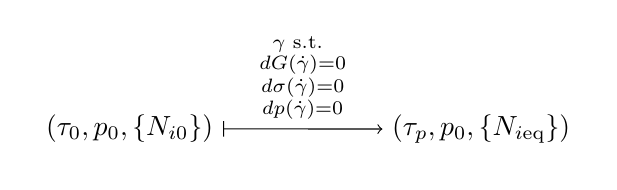
\begin{tikzpicture}
  \matrix (m) [matrix of math nodes, row sep=4.8em, column sep=5.8em, minimum width=2.2em]
  {
(\tau_0,p_0,\lbrace N_{i0} \rbrace) & (\tau_p, p_0, \lbrace N_{i \text{eq} } \rbrace)   \\ 
};
  \path[|->]
  (m-1-1) edge node [above] {$ \substack{  \gamma \text{ s.t. } \\ dG(\dot{\gamma}) = 0 \\ d\sigma(\dot{\gamma}) = 0 \\ dp(\dot{\gamma})=0   } $} (m-1-2);
\end{tikzpicture} 
\end{gathered}
\]
and if we wanted enthalpy to remain constant,
\[
\begin{gathered}
 \begin{tikzpicture}
  \matrix (m) [matrix of math nodes, row sep=4.8em, column sep=5.8em, minimum width=2.2em]
  {
\Sigma & \Sigma \\ 
};
  \path[->]
  (m-1-1) edge node [above] {$ \gamma $} (m-1-2);
\end{tikzpicture}  \\
 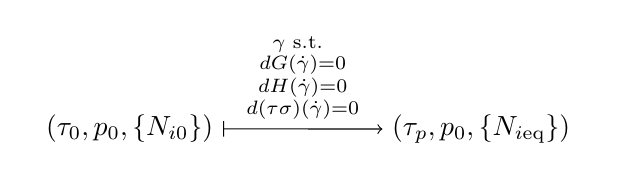
\begin{tikzpicture}
  \matrix (m) [matrix of math nodes, row sep=4.8em, column sep=5.8em, minimum width=2.2em]
  {
(\tau_0,p_0,\lbrace N_{i0} \rbrace) & (\tau_p, p_0, \lbrace N_{i \text{eq} } \rbrace)   \\ 
};
  \path[|->]
  (m-1-1) edge node [above] {$ \substack{  \gamma \text{ s.t. } \\ dG(\dot{\gamma}) = 0 \\ dH(\dot{\gamma}) = 0 \\ d(\tau \sigma)(\dot{\gamma})=0   } $} (m-1-2);
\end{tikzpicture} 
\end{gathered}
\]
I think what we want, since the flow was shown to be isentropic, and, again, as Oates \cite{GOates1997} argued, that local equilibrium leads to equilibrium in all modes of energy storage, chemical bonds, vibrational modes, to translational modes, that the total entropy of the fluid remains constant, this:
\[
\begin{gathered}
 \begin{tikzpicture}
  \matrix (m) [matrix of math nodes, row sep=4.8em, column sep=5.8em, minimum width=2.2em]
  {
\Sigma & \Sigma \\ 
};
  \path[->]
  (m-1-1) edge node [above] {$ \gamma $} (m-1-2);
\end{tikzpicture}  \\
 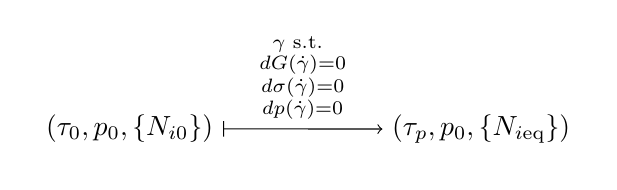
\begin{tikzpicture}
  \matrix (m) [matrix of math nodes, row sep=4.8em, column sep=5.8em, minimum width=2.2em]
  {
(\tau_0,p_0,\lbrace N_{i0} \rbrace) & (\tau_p, p_0, \lbrace N_{i \text{eq} } \rbrace)   \\ 
};
  \path[|->]
  (m-1-1) edge node [above] {$ \substack{  \gamma \text{ s.t. } \\ dG(\dot{\gamma}) = 0 \\ d\sigma(\dot{\gamma}) = 0 \\ dp(\dot{\gamma})=0   } $} (m-1-2);
\end{tikzpicture} 
\end{gathered} 
\]

\subsubsection{Continuity equations for equilibrium flow}

The continuity equations to use for equilibrium flow should be (correct me if I'm wrong) are
\[
\dot{m} = \rho u A
\]
for which $\dot{m}$ should be constant at each point along the 1-dimensional flow (out) by mass conservation (which should still should hold for chemical reactions).  

One possible form of mass conservation that could prove useful is 
\[
\rho_2u_2 A_2 = \rho_1 u_1 A_1 \text{ or } \frac{A_2}{A_1} = \frac{ \rho_1 u_1}{\rho_2 u_2}
\]

Also, throughout the flow, the Bernoulli invariant is $h+k$, i.e.
\[
\frac{u_2^2}{2} + h_2 = \frac{u_1^2}{2} + h_1 \text{ or } u_2^2 = u_1^2 + 2(h_1 -h_2)
\]
Note that the speed of sound $a^2 = \left( \frac{ \partial \rho }{ \partial p} \right)_{\sigma,\lbrace N_i \rbrace}$ can be calculated at each instance, and so the Mach number can be calculated: 
\[
\mathfrak{M} = \frac{u}{a}
\]

\subsection{Frozen flow}

Note that there are a number of critical typos in Martinez-Sanchez (2005) \cite{MMartinez-Sanchez2005} that makes it difficult to understand, in this case, Lecture 14.  

Given nozzle exit (i.e. entering combustion chamber), pressure $p_c$, and consider chamber entropy $\sigma_c$.  Then $(\sigma_c,p_c)$ specifies completely the thermodynamic state, and so enthalpy (or specific enthalpy) $h_c$ is specified.  
\[
(\sigma_c, p_c) \mapsto h_c(\sigma_c,p_c)
\]
For adiabatic flows, the energy equation (for steady state) is
\[
\frac{u_2^2}{2} = h_c - h_2
\]
In general, for multiple number of species, 
\[
(\sigma_c, p_c; \lbrace N_i \rbrace_{i=1 \dots \mathcal{N} } ) \mapsto h_c(\sigma_c,p_c; \lbrace N_i \rbrace)
\]

For throat conditions, consider mass flow $\dot{m} = \rho uA$.  

Assuming steady state (EY: 20160210 check if throat conditions necessitates $\dot{m}=0$), then 
\[
\begin{gathered}
  \begin{gathered}
  \frac{d\rho}{\rho} + \frac{du}{u } + \frac{dA}{A} = 0 
  \end{gathered} \Longrightarrow \frac{du}{u} = -\frac{dh}{ 2(h_c - h) } = \frac{-dp}{2 \rho (h_c- h) } = \frac{-dp }{ \rho u^2} \text{ since } \\
  u du = -dh \text{ and } \\
  dh = \tau ds + \frac{1}{\rho } dp + \frac{h}{\rho} d\rho \text{ and for this thermodynamic process $ds=d\rho =0$ in the fluid-at-rest frame }
\end{gathered}
\]
At the throat, $dA=0$ (by definition of a throat), and so \[
\frac{d\rho }{ \rho } = -\frac{du}{u} = \frac{dp}{\rho u^2} \Longrightarrow (u^*)^2 = \left( \frac{ \partial p}{ \partial \rho} \right)_{\sigma}
\]

Also, consider from mass conservation, that, at the throat, $dA =0$, 
\[
\begin{gathered}
  d(\rho u )A + \rho u dA = 0 \\
  \Longrightarrow \frac{d(\rho u)}{ \rho u} + \frac{dA}{A} = 0 \xrightarrow{ dA = 0 } d(\rho u)=0
\end{gathered}
\]
$\rho u$ is at a \emph{maximum} at the throat.  

\subsection{Implementation in Cantera of equilibrium flow and frozen flow}

The first thing that happens is \emph{combustion}!  Fuel and oxidizer enters through inlets into combustion chamber.  Then combustion occurs in the (combustion) chamber!
\[
\begin{gathered}
 \begin{tikzpicture}
  \matrix (m) [matrix of math nodes, row sep=4.8em, column sep=5.8em, minimum width=2.2em]
  {
\Sigma & \Sigma \\ 
};
  \path[->]
  (m-1-1) edge node [above] {$ \gamma $} (m-1-2);
\end{tikzpicture}  \\
 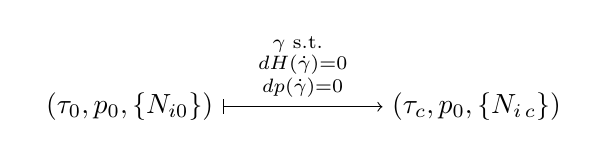
\begin{tikzpicture}
  \matrix (m) [matrix of math nodes, row sep=4.8em, column sep=5.8em, minimum width=2.2em]
  {
(\tau_0,p_0,\lbrace N_{i0} \rbrace ) & (\tau_c, p_0, \lbrace N_{i \,  c } \rbrace)   \\ 
};
  \path[|->]
  (m-1-1) edge node [above] {$ \substack{  \gamma \text{ s.t. } \\ dH(\dot{\gamma}) = 0 \\  dp(\dot{\gamma})=0   } $} (m-1-2);
\end{tikzpicture} 
\end{gathered} 
\]
and $dH(\dot{\gamma}) =0$ since $H_P(\tau_c)=H_R(\tau_0)$ so $\Delta H \equiv H_p(\tau_c)-H_R(\tau_0) = 0$

$h(\sigma_c, p_0, \lbrace N_{i \, c} \rbrace_i ) \equiv h_0 \in C^{\infty}(\Sigma)$ and $h_0$ is the stagnation enthalpy, used as the Bernoulli invariant in the energy equation (i.e. $\frac{u^2}{2} = (h_0-h)$).  

Then consider isentropic flow $\gamma_{\text{isent}}$:
\[
\begin{gathered}
 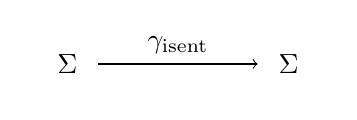
\begin{tikzpicture}
  \matrix (m) [matrix of math nodes, row sep=4.8em, column sep=5.8em, minimum width=2.2em]
  {
\Sigma & \Sigma \\ 
};
  \path[->]
  (m-1-1) edge node [above] {$ \gamma_{\text{isent}} $} (m-1-2);
\end{tikzpicture}  \\
 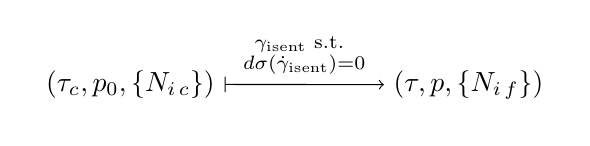
\begin{tikzpicture}
  \matrix (m) [matrix of math nodes, row sep=4.8em, column sep=5.8em, minimum width=2.2em]
  {
(\tau_c,p_0,\lbrace N_{i\, c} \rbrace ) & (\tau, p, \lbrace N_{i \,  f } \rbrace)   \\ 
};
  \path[|->]
  (m-1-1) edge node [above] {$ \substack{  \gamma_{\text{isent}} \text{ s.t. } \\ d\sigma(\dot{\gamma}_{\text{isent}}) = 0    } $} (m-1-2);
\end{tikzpicture}  \\
 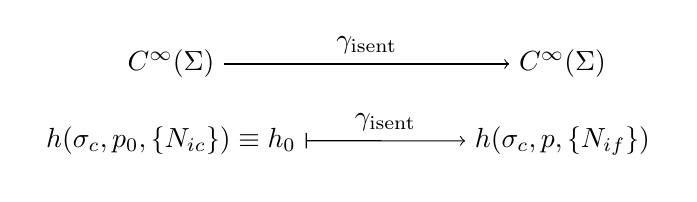
\begin{tikzpicture}
  \matrix (m) [matrix of math nodes, row sep=1.1em, column sep=5.8em, minimum width=2.2em]
  {
    C^{\infty}(\Sigma) & C^{\infty}(\Sigma) \\ 
    h(\sigma_c,p_0,\lbrace N_{ic} \rbrace ) \equiv h_0 & h(\sigma_c,p,\lbrace N_{if} \rbrace ) \\
};
  \path[->]
  (m-1-1) edge node [above] {$ \gamma_{\text{isent}} $} (m-1-2);
  \path[|->]
  (m-2-1) edge node [above] {$\gamma_{\text{isent}}$} (m-2-2);
\end{tikzpicture} 
\end{gathered} 
\]
How I implemented this in Cantera is by setting the state of the gas to the desired $p$, and then equilibrating the gas under constant entropy $\sigma_c$ and constant pressure $p$.  

\subsubsection{Getting the results for rocket (and nozzle) performance (i.e. collecting the dividends)}

You want to calculate the specific impulse (for the rocket).  Use this handy relation:
\[
\begin{gathered}
  gI_{\text{sp}} = \frac{F}{\dot{m}} = \frac{\dot{m} u_{\text{exh}} + (p_{\text{exh}}-p_a)A_e }{ \rho_{\text{exh}} u_{\text{exh}} A_e} = u_{\text{exh}} + \frac{p_{\text{exh}} - p_a}{ \rho_{\text{exh}} u_{\text{exh}} }
\end{gathered}
\]
and $\dot{m} = \rho^* u^* A^*$.  

\section{Dynamic pressure}

cf. \href{https://www.grc.nasa.gov/WWW/K-12/airplane/dynpress.html}{NASA Glenn Research Center, "Dynamic Pressure"}

From the NASA Glenn Research Center website link, here's how they started their derivation: \\
By fluid momentum conservation:
\begin{equation}
\frac{-dp}{dx} = \rho u \frac{du}{dx}
\end{equation} 
where \\
$p\equiv $ pressure \\
$\rho \equiv$ density. \\

If $u \in \mathbb{R}$, 
\[
\begin{gathered}
	\frac{dp}{dx} + \rho u \frac{du}{dx} = \frac{d}{dx} (p + \frac{1}{2} \rho u^2 ) = 0 \Longrightarrow p_s + \frac{1}{2} \rho u^2 = \text{ constant } = p_{\text{tot}}
\end{gathered}
\]
where \\
$p_{\text{tot}} := $ total pressure \\
$p_s := $ static pressure \\
$q := $ dynamic pressure $= \frac{1}{2} \rho u^2$. \\

If a gas is static and not flowing the measured pressure is the same in all directions. \\
If gas is moving, measured pressure depends on direction of motion. 

\begin{equation}
p_s + \frac{1}{2} \rho u^2 = p_{\text{tot}, 0}
\end{equation}
\emph{looks like} incompressible Bernoulli's equation.

$\frac{1}{2} \rho u^2$ is called dynamic pressure because it's a pressure term associated with velocity of the flow. \\
Dynamic pressure is a defined property of moving flow of gas. \\
We can use and apply idea of dynamic pressure in much more complex flows, like compressible flows or viscous flows. Particularly, aerodynamic forces acting on object as it moves through air are directly proportional to dynamic pressure. \\
By measuring dynmaic pressure in flight, pitot-static tube (Prandtl tube) can be used to determine aircraft airspeed.

My question is this: how does this derivation change if we can't assume flow is uniform and we can't assume flow is all in 1-dimension (i.e. it has non-zero velocity components in the "other" direction)?

Recall Navier-Stokes for compressible, viscous fluid flow:
\[
\rho \left( \frac{ \partial u^i }{ \partial t} + u^j \frac{\partial u^i }{ \partial x^j} \right) = \frac{- \partial p }{ \partial x^i } + ( \lambda +\mu) \frac{\partial }{ \partial x^i } \text{div}u + \mu \Delta u^i
\]
If $\mu =0$, $\text{div}u = 0$ and $\frac{\partial u^i}{\partial t} = 0$ (steady state),
\[
\rho_0 u^j \frac{\partial u^i}{\partial x^j} + \frac{ \partial p}{\partial x^i} = 0
\]
For $j=i$, $\frac{\partial }{ \partial x^i} (\frac{1}{2} \rho_0 (u^i)^2 + p) + \sum_{j\neq i} \rho_0 u^j \frac{\partial u^i}{\partial x^j } = 0$


\part{Electromagnetism}


cf. 1-2 Exhaust velocity and Specific Impulse of Jahn (2006) \cite{Jahn2006}

Jahn (2006) \cite{Jahn2006} defines specific impulse $I_s$ as the ratio of thrust to the rate of use of propellant by sea level weight:
\begin{equation}
  I_s := \frac{ T}{ \dot{m}g_0}
\end{equation}

\problemhead{1-4} It should be pointed out that the physics is exactly the same as before as propelling mass out, \emph{before} separation.  What's different is the final mass after all planned for propellant mass is expelled is different.

To review,  \\

Let $M=M(t)$ the mass of the entire system at any time, only excluding propellant mass that's \emph{already} expelled out.  

$M\dot{u} = -\dot{M}u_{\text{exh}} + F_g$.  For the case of $F_g = -Mg$,
\[
\begin{gathered}
  \dot{u} = \frac{-\dot{M}}{M} u_{\text{exh}} + \frac{F_g}{M} = \frac{-\dot{M}}{M} u_{\text{exh}} + -g \\
  \xrightarrow{ \int dt } \Delta u \equiv u(t_f) - u(0) = -\ln{ \left( \frac{M(t_f)}{M(0)} \right)}u_{\text{exh}} - gt_f \\
  \Longrightarrow \frac{\Delta u}{ u_{\text{exh}}} + \frac{ g\Delta t }{ u_{\text{exh}} } = \ln{ \left( \frac{M(0) }{ M(t_f)} \right)} \text{ or } \exp{ \left( \frac{ \Delta u}{ u_{\text{exh}} } \right) } \exp{ \left( \frac{ g \Delta t}{ u_{\text{exh}} } \right) } = \frac{ m_0 }{ M(t_f) }
\end{gathered}
\]
where $t_f \equiv \Delta t$ and $m_0 \equiv M(0)$ (Jahn's notation in the former, my notation for the latter).   

Now the mass of the power supply, $m_p$ was given by Jahn and reasoned to monotonically depend on the power $P$, which is reasonable.  Also, we have $M(0)$, and $M(t_f) \equiv  M(\Delta t)$ values:
\[
\begin{gathered}
  m_p = \alpha P = \alpha \frac{ T u_{\text{exh}} }{ 2\eta} = \frac{ \alpha \dot{m} u^2_{\text{exh}} }{ 2 \eta} \\ 
  M(\Delta t) = m_u + m_p = m_u + \frac{ \alpha }{2\eta} \frac{M_p}{\Delta t} u^2_{\text{exh}} \\ 
  m_0 \equiv M(0) = M_p + m_u + m_p = M_p + m_u + \frac{ \alpha \dot{m} u^2_{\text{exh}} }{ 2\eta} = \\
  = M_p + m_u + \alpha \left( \frac{ M_p }{ \Delta t} \right) \frac{u^2_{\text{exh}} }{ 2\eta}  \\
  \Longrightarrow M_p = \frac{m_0 - m_u }{ 1 + \frac{ \alpha u^2_{\text{exh}} }{ 2\eta \Delta t} } 
\end{gathered}
\]
for $\dot{m}\Delta t = M_p$ (\emph{assume constant} mass flow out, and by $\Delta t$ time, $M_p$ mass propellant is used up).

Plugging all this in:
\[
\begin{gathered}
  \exp{ \left( \frac{ \Delta u}{ u_{\text{exh}} }\right) } \exp{ \left( \frac{ g\Delta t}{ u_{\text{exh}} } \right) } = \frac{m_0 }{ m_u + \frac{ \alpha}{2\eta \Delta t} \left( \frac{m_0 - m_u }{ 1 + \frac{ \alpha u^2_{\text{exh}} }{ 2 \eta \Delta t} } \right) u^2_{\text{exh}} } = \frac{ 1 + \frac{ \alpha u^2_{\text{exh} }}{ 2 \eta \Delta t} }{ \frac{m_u}{m_0} + \frac{ \alpha u^2_{\text{exh}} }{ 2\eta \Delta t} }
  \end{gathered}
\]
Let $g=0$.  Then the desired result is obtained, for ratio of mass payload to initial mass, including a power supply:
\begin{equation}
  \frac{m_u}{m_0} = e^{-\Delta u / u_{\text{exh}} } + \frac{ \alpha u_{\text{exh}}^2}{2\eta \Delta t} ( e^{ -\Delta u / u_{\text{exh}} } - 1 )
\end{equation}




\subsection{Charge conservation}

Recall that the divergence $\text{div}$:
\[
\begin{aligned}
  & \text{div}: \mathfrak{X}(M) \to C^{\infty}(M) \\
  & \text{div}\mathbf{j} = \frac{1}{\sqrt{g}} \frac{ \partial ( j^k \sqrt{g} ) }{ \partial x^k} 
\end{aligned}
\]
Usually, charge conservation is written in differential vector form as
\[
\frac{ \partial \rho }{ \partial t} + \text{div}\mathbf{j} = 0 
\]
Does this hold for the differential form version of electromagnetism?

Consider $j \in \Omega^1(M)$.  Now
\[
j = j_{\mu} dx^{\mu} = \rho dt + j_i dx^i \in \Omega^1(M) \xmapsto{ \#} g^{\mu \nu} j_{\nu} \frac{ \partial }{ \partial x^{\mu } } \equiv j^{\mu} \frac{ \partial }{ \partial x^{\mu }} \in \mathfrak{X}(M)
\]
Then
\[
\begin{gathered}
  *j = \frac{ \sqrt{g}}{3!} \epsilon_{\mu \nu \rho \sigma} g^{\mu \mu_1} j_{\mu_1} dx^{\nu} \wedge dx^{\rho} \wedge dx^{\sigma} \\ 
  d*j = \frac{1}{3!} \epsilon_{\mu \nu \rho \sigma} \frac{ \partial }{ \partial x^{\mu_2} }(\sqrt{g} g^{\mu \mu_1} j_{\mu_1} ) dx^{\mu_2} \wedge dx^{\nu} \wedge dx^{\rho} \wedge dx^{\sigma} = \frac{1}{3!} \epsilon_{\mu \nu \rho \sigma} \frac{ \partial}{ \partial x^{\mu_2} } (\sqrt{g} j^{\mu } ) dx^{\mu_2} \wedge dx^{\nu} \wedge dx^{\rho} \wedge dx^{\sigma} = \\
  = \frac{1}{3!} \lbrace \epsilon_{ijk} \frac{ \partial ( \sqrt{g}j^0  ) }{ \partial t} dt \wedge dx^i \wedge dx^j \wedge dx^k + \epsilon_{ijk} \frac{ \partial }{ \partial x^l} ( \sqrt{g}j^i )  dt \wedge dx^l \wedge dx^j \wedge dx^k + \dots \rbrace = 0  \\
  \Longrightarrow \frac{1}{\sqrt{g}} \frac{ \partial (\sqrt{g} j^0  ) }{ \partial t} + \text{div}\mathbf{j} = \frac{1}{\sqrt{g}} \frac{ \partial ( \sqrt{g} g^{0 \mu } j_{\mu } ) }{ \partial t} + \frac{1}{\sqrt{g}} \frac{ \partial ( \sqrt{g} g^{k\mu } j_{\mu} ) }{ \partial x^k }  = 0 
\end{gathered}
\]
Suppose current is a \textbf{convective current} $\mathbf{j} = \rho \mathbf{u}$, where $\mathbf{u} \in \mathfrak{X}(M)$ ($\mathbf{u} = \mathbf{u}(t,x)$, $(t,x) \in M$).

Charge conservation always holds.  


my version of Maxwell's equations:

if $\mathbf{\nabla} \cdot \mathbf{B} = 0$, \\
then $\mathbf{\nabla} \times \mathbf{E} = \frac{-1}{c} \left( \frac{ \partial \mathbf{B} }{ \partial t} \right)$

if $\mathbf{\nabla} \cdot \mathbf{E} = 4\pi \rho_{\text{total}}$ \\
then $\mathbf{\nabla} \times \mathbf{B} = \frac{1}{c} \left( \frac{ \partial \mathbf{E} }{ \partial t} + 4\pi \frac{ \partial \mathbf{P} }{ \partial t} + 4\pi \mathbf{J}_{\text{free}} + 4\pi c \mathbf{\nabla}\times \mathbf{M}\right)$


% Rachel 1.  

cf. Section 1.4 Coulomb's law of Purcell (1984) \cite{Purcell1984}.

For $\mathbf{F}_2 = $ force on charge 2,
\[
\mathbf{F}_2 = \frac{k q_1 q_2 \mathbf{r}_{21} }{ r_{21}^2 } = \frac{k q_1 q_2 (\mathbf{r}_2 - \mathbf{r}_1 ) }{ | \mathbf{r}_2 - \mathbf{r}_1 |^3}
\]

I am curious to know if the tangent-cotangent (``musical'') isomorphism holds:
\[
F_2^i = \frac{ kq_1 q_2 (\mathbf{r}_2 - \mathbf{r}_1)^i }{ |\mathbf{r}_2 - \mathbf{r}_1 |^3 } \in \mathfrak{X}(M) \xmapsto{ \flat } (F_2)_j = \frac{k q_1 q_2 (\mathbf{r}_2 - \mathbf{r}_1)^i g_{ij} }{ | \mathbf{r}_2 - \mathbf{r}_1 |^3 } \in \Omega^1(M)
\]
$k=1$ \, (cgs) \\
$k = \frac{1}{4\pi \epsilon_0}$; $\epsilon_0 = 8.85 \times 10^{-12}$ ; $k = 8.988 \times 10^9$ \, (SI)

$1$ coulomb $=  2.998 \times 10^9 $ \, esu $\cong 3 \times 10^9 \, $ esu \\
$\epsilon_0 = 4.8 \times 10^{-16}$ esu $ = 1.6 \times 10^{-16} \, C$ \\
$10^5$ dynes $=1 $ Newtons.  

So the above takes care of Ch. 2 Electromagnetic Theory, Section 2-1 Electric Charges and Electrostatic Fields of Jahn (2006) \cite{Jahn2006} up to Eqn. (2-1).  


Section 3.5 Capacitance and Capacitors of Purcell (1984) \cite{Purcell1984}.

Consider an isolated conductor carrying charge $Q$.
\[
Q = C\phi_0
\]
cgs.  $[Q] = $ esu, $[C] = $ cm, $[\phi_0] = $ statvolts $= \frac{ \text{ergs}}{\text{esu}} = \frac{ \text{dyne}\cdot \text{cm}}{ \text{esu} }$.  \\
SI. $[Q]=$ coulombs, \, $[C] = $ farads, $[\phi] = $ volts.  


%\setlength{\unitlength}{1mm}
\[
\begin{gathered}
\begin{picture}(8,5)(0,0)
  \put(4,4){\circle{7.5}}
  \put(4,4){$Q$}
\end{picture}
\qquad \qquad \,
\begin{picture}(8,5)(0,0)
  \put(.7,4.7){\line(1,0){6}}
  \put(.7,4.0){\line(1,0){6}}
  \end{picture}
\end{gathered}
\]

cgs: $C=a$ \, $[a] = m$ \qquad \, $ C = \frac{A}{4\pi s}$ $[A] = \text{cm}^2$, $[s] = \text{cm}$

SI: $C=4\pi \epsilon_0 a$  \, $[a] = m$ \qquad \, $ C = \frac{\epsilon_0 A}{ s}$ $[A] = \text{m}^2$, $[s] = \text{m}$

$\epsilon_0 = 8.854 \times 10^{-12} \, \text{farad}/\text{meter}$
\[
\boxed{ 1 \, \text{cm} = 1.11 \times 10^{-12} \, \text{ farad }} 
\]



Fitzpatrick (2014) \cite{Fitz2014}

\part{Physical Kinetics}



Pitaevskii and Lifshitz (1981) \cite{PL1981}




Sonnendr\"{u}cker (2017) \cite{Sonn2017}.  

\part{Guidance, Navigation, and Control (GNC)}

\section{Software for modeling and execution}

\subsection{Matlab/Simulink and alternatives}

\subsubsection{Open source alternatives}

GNURadio for digital signal processing (cf. Nick C.)

In image processing, Matlab replaced with Python (openCV, numpy, PIL, other great modules) (cf. Katharine I.)

Modelica - has fairly good documentation with examples, has standard library that may or may not be surface level of domain of interest. Has FMI support, allowing saving models/simulations in standardized plain text data. (cf. Sean M.)

Use of Matlab is very team oriented (meaning very specific to the team's needs?) For example for Power Electronics, LTSpice is used, as well for PCB simulations. Simulink is good for model building and doing complex systems. (cf. Amir K.)

\part{Orbital Mechanics}

cf. Wie (2008) \cite{BWie2008}


\part{GPS, Geodesy} 

D. K. Olson, "Converting Earth-Centered, Earth-Fixed Coordinates to Geodetic Coordinates" IEEE Transactions on Aerospace and Electronic Systems, 32 (1996) 473-476 Olson algorithm

\section{Geodesy}

\part{Real-time systems}

\section{Partial Ordering of Events in a Distributed System}

cf. pp. 558, Communications of the ACM, July 1978, Vol. 21, Number 7, Lamport (1978) \cite{Lamp1978}

Assume system composed of a collection of processes. Each process consists of a sequence of events.

A single process is defined to be a set of events with an a priori total ordering.

Recall for set $P$, ordering $\leq$, then $(P, \leq)$ \textbf{partially ordered} if 
\begin{enumerate}
	\item reflexivity: $a \leq a$
	\item anti-symmetry: $(a\leq b \text{ and } b\leq a) \to a = b$
	\item transitive: $a\leq b$ and $b\leq c$ $\Longrightarrow a \leq c$
\end{enumerate}

We can extend our definition to allow a process to split into distinct subprocesses (EY: if needed).

Assume sending or receiving a message is an event in a process.

define "happened before" relation:

\begin{definition}["happened before" relation]\label{Def:HappenedBeforePartialOrdering}
	Given set of events $E$ of a system, with set of event $P\subseteq E$ s.t. $\forall \, $ event $\in P$ is on the same process $P$, \\
	relation $ <_p$ (Lamport's notation is "$\to$") is the "smallest" relation s.t.
	
	\begin{enumerate}
		\item irreflexivity: $a \not<_p a$ \, $\forall\, a \in E$ (interpret: event cannot happen before itself)
		\item concurrency: if $a \not<_p b$ and $b\not<_p a$, then $a,b$ \textbf{concurrent}.
		(contrapositive to concurrency) $a,b$ not concurrent if $a <_p b$ or $b<_p a$ \\
		
		EY: compare this with anti-symmetry, if $a \leq_p b$ and $b\leq_p a$, then $a =_p b$; this conclusion requires from concurrency that if $a \not<_p b$, then $b\leq_p a$. Then consider the extra claim that $a\leq_p b$ is equivalent to $a <_p b$ or $a =_p b$ (concurrent).
		\item transitivity: if $a<_p b$ and $b<_p c$, then $a<_pc$ \\
		
		Can be shown that if $a\leq_p b$ and $b\leq_pc$, then $a\leq_p c$ (consider all permutations/cases: if $a=_p b$, $b=_pc$, then $a=_pc$, if $a=_p b$, $b<_p c$, then $a<_p c$, \dots)
	\end{enumerate}
Intepret: $\forall a, b \in P$ (interpret $a,b$ are events in the same process), $a<_p b$ means $a$ comes before $b$. 

Interpret, if processes $P, Q \subset E$, and event $a$ is sending of a message by process $P$, and event $b$ is receipt of same message by another process $Q$, then $a <_p b$.
\end{definition}

EY: if $a \not<_p b$, equivalent to $b \leq_p a$, $\forall \, a, b\in E$, then $a \leq_p a$, \, $\forall \, a \in E$, if $a\leq_p b$ and $b\leq_p a$, then $a=_p b$, and $a\leq_p b$ and $b\leq_p c$, then $a \leq_p c$. \\
So if $a \not<_p b$ equivalent to $b\leq_p a$, and $a=_p b$ is equivalent to concurrency, $<_p$ \textbf{implies partial ordering} $\leq_p$.

Also consider for $<_p$ in Def. \ref{Def:HappenedBeforePartialOrdering} to be interpreted in terms of causation, and two events are concurrent if neither can causally affect the other.

\section{Logical clocks}

cf. pp. 559, Communications of the ACM, July 1978, Vol. 21, Number 7, Lamport (1978) \cite{Lamp1978}

Introduce clocks in the system.

Begin with abstract point of view such that clock is just a way of assigning number to an event, where number is thought of as time at which event occurred. 

Define $\forall $ process $P_i$, a clock $C_i$, 
\begin{equation}
\begin{aligned}
	& C_i : P_i \to \mathbb{R} \text{ or } \mathbb{Z} \\ 
	& C_i: P_i \to \mathbb{Z} \text{ for system clock or digital computer clock }
\end{aligned}
\end{equation}

For clock $i$ on process $i$, i.e. clock $C_i$ for each process $P_i$, then $\forall \, $ event $a\in P_i$, 
\begin{equation}
C_i\langle a \rangle \in \mathbb{Z}
\end{equation}

Entire system of clocks represented by mapping $C$ s.t. 
\begin{equation}
\begin{aligned}
& C: b \mapsto C \langle b \rangle \\
& C\langle b \rangle = C_j\langle b \rangle \text{ if $b$ is an event in process $P_j$ }
\end{aligned}
\end{equation}

("For now") we make no assumption about the relation of the numbers $C_i\langle a \rangle$ to physical time, so we can think of clocks $C_i$ as logical rather than physical clocks. They maybe implemented by counters with no actual timing mechanism.

Base definition on \textbf{order in which events occur}; we cannot base our definition of correctness on physical time, since that would require introducing clocks which keep physical time.

Lamport makes this strongest reasonable condition: if an event $a$ occurs before another event $b$, then $a$ should happen at an earlier time than $b$:

\begin{proposition}[Clock Condition]\label{Prop:ClockCondition}
	$\forall \, $ events $a,b \in E$, \\if $a <_p b$, then $C\langle a \rangle < C \langle b \rangle$
\end{proposition}

Lamport says that we can't expect converse condition, since that'd imply any 2 concurrent events must occur at the same time: \\
(converse to Prop. \ref{Prop:ClockCondition}) if $a \not<_p b$, then $C\langle a \rangle \geq C\langle b \rangle$ or if $a =_p b$ or $a >_p b$, then $C\langle a \rangle \geq C\langle b\rangle$. Further, if $a \not>_p b$, then this implies $C\langle a \rangle = C\langle b \rangle$ (since it cannot be that $C\langle a \rangle > C\langle b \rangle$, we eliminated this possibility out of the two implied by $a \geq_p b$). But we \emph{don't want} for 2 concurrent events to necessarily have equal times (because  who's to say that they must occur at the same time).

e.g. On process $P$, $p_2 <_p p_3$, and $C_p(p_2) < C_p(p_3)$, because events on the same process are totally ordered.

Given,
\[
\begin{aligned}
& p_1 <_p q_2 \\
& q_1 <_p p_2 \\
& q_2 <_p q_3
\end{aligned}
\]
$p_2 \not<_p q_2$ and $q_2 \not<_p p2$, and since $q_2 < q_3$, then \\
since $p_2 \nrightarrow q_3$ and $q_2 \nrightarrow p_3$, $p_2, q_3$ concurrent. \\
since $p_3 \nrightarrow q_3$ and $q_3 \nrightarrow p_3$, $p_3, q_3$ concurrent.

Clock condition is satisfied if  
\begin{proposition}[Clock conditions 1, 2] 
\begin{enumerate}
	\item[C1] If $a,b \in $ process $P_i$, and $a<b$; $C_i\langle a \rangle < C_i \langle b \rangle$ 
	\item[C2] If $a$ is sending a message by process $P_i$ and $b$ is receipt of that message by process $P_j$, then $C_i\langle a \rangle < C_j \langle b \rangle$
\end{enumerate}
\end{proposition} 
cf. pp, 560, Lamport (1978) \cite{Lamp1978}

Let's assume that processes are algorithms, and events represent certain actions during their execution. Process $P_i$'s clock is represented by $C_i$ during event $a$. 

For condition C1, if $a,b \in P_i$, $a<_p b$, then $C_i(a) < C_i(b)$, so then processes need to obey the following

\begin{proposition}[Implementation Rule 1 (IR1)]\label{IR1}
Each process $P_i$ increments $C_i$ between any 2 successive events.

EY (20210408) i.e. $\forall $ process $P_i$, let sequence of events $a_k \in P_i$ s.t. $\forall \, a_k$ totally ordered on $P_i$, i.e. $a_k <_p a_{k+1}$, \, $\forall \, k$, then
\begin{equation}
\boxed{ 
	C_i(a_k) < C_i(a_{k+1}) = C_i(a_k) + 1 }
\end{equation}
\end{proposition} 

To meet condition C2, if $a$ sends message by process $P_ii$, $b$ receives same messsage by process $P_j$, then 
\[
C_i(a) < C_j(b)
\]

We require that each message $m$ contain a timestamp $T_m$ which equals the time at which message was sent.\\
\emph{Upon receiving a message} timestamped $T_m$, a process must advance its clock to be later than $T_m$, More precisely,

\begin{proposition}[Implementation Rule 2 (IR 2)]
\begin{enumerate}
	\item If event $a$ sends message $m$ by process $P_i$, then message $m$ contains timestamp $T_m = C_i\langle a \rangle$
	\item Upon receiving a message $m$, process $P_j$ sets $C_j$ greater than or equal to its present value and greater than $T_m$
\end{enumerate}

EY (20210408), i.e. \\

If event $ a\in P_i$ sends message $m_a$ contains timestamp $T_a = C_i(a)$ \\
Upon receiving message $m_a$, event $r_a$, process $P_j$ sets 
\begin{equation}
\boxed{
	C_j(r_a) = \max{ (C_j(r_a), T_a)} + 1
}
\end{equation} 
The addition, increment, of 1 makes sense since the message can never be received before or at the same time of sending it (cf. \href{https://towardsdatascience.com/understanding-lamport-timestamps-with-pythons-multiprocessing-library-12a6427881c6}{Steven Van Dorpe})

(remember that $C_j(r_a) = C_j(q) + 1$ where $q$ is event immediately before $r_a$, $q <_p r_a$ (and no other event))

\end{proposition}
IR2 insures C2 satisfied; hence IR1, IR2 imply Clock Condition satisfied.


\subsection{Ordering Events Totally}

Define relation $\Longrightarrow$. \\
Use any arbitrary total ordering $<_{(P)}$ of the processes to break ties. \\
If event $a$ in process $P_i$, event $b$ in process $P_j$, then $a \Longrightarrow b$ iff either 
\begin{enumerate}
	\item $C_i\langle a \rangle < C_j \langle b \rangle $ or 
	\item $C_i \langle a \rangle < C_j \langle b \rangle$ and $P_i < P_j$ 
\end{enumerate}
ordering $\Longrightarrow$ depends upon system of clocks $C_i$ and is not unique.

Example: use total ordering of events solving the following version of the \emph{mutual exclusion problem} (EY: mutex?).

Consider system composed of fixed collection of processes $P_i$, (e.g. $N=1$, $P$, e.g. $N=2$, $P_i$, $P_j$). Processes share a \emph{single} resource (resource is external, not part of any of the processes, to any of the processes, I believe). 

We wish to find an algorithm satisfying following 3 conditions:
\begin{enumerate}
	\item[(I)] A process $P_i$ which has been granted \emph{the} resource must release it before it can be granted to another process $P_j$ 
	\item[(II)] Different requests for \emph{the} resource must be granted in order in which they're made
	\item[(III)] If every process which is granted the resource eventually releases it, then every request is eventually granted
\end{enumerate}

Implement:

Each  process maintains own request queue which is never seen by any other process.

\begin{enumerate}
	\item To request resource, process $P_i$, sends $T_m:P_i$ "requests resource" to every other process (e.g. if $N=2$, to $P_{i+1}$; if $N=1$, no send) \emph{and} \\
	puts \emph{that message} $T_m:P_i$ "requests resource" on its request queue
	\item When process $P_j$ receives message $T_m:P_i$ "requests resource", it places it on its request queue \emph{and} \\
	sends (timestamped) acknowledgement message to $P_i$ ($N=1$ none, $N=2$, $P_j$ receives and sends ack to $P_i$)
	\item To release resource $P_i$ remorses \emph{any} $T_m: P_i$ "requests resource" message from its request queue, \emph{and} \\
	sends (timestamped) $P_i$ "releases resource" message to every other process ($N=1$, removes all $T_{m'}:P_i$ "requests resource" messages; $N=2$, $P_i$ removes any $T_m:P_i$ "requests resources" and $P_j$ gets sent $T_{m'}:P_i$ "releases resource")
	\item When $P_j$ receives $P_i$ "releases resource", removes any $T_m:P_i$ "requests resource" message from its request queue.
	\item $P_i$ granted resource if 
	\begin{enumerate}
		\item[(i)] $\exists \, T_m: P_i$ "requests resource" message in its request queue ordered before any \emph{other request}
		\item[(ii)] $P_i$ received message from $\forall \, P_{i'}$ timestamped later than $T_m$ ($N=1$, none; $N=2$, $P_i$ received ack (acknowledgement) from $P_j$ at $T_{m'} > T_m$)
	\end{enumerate}
\end{enumerate}

5(ii) $\to$ guarantees $P_i$ has learned about all requests which preceded its current request \\
rules 3,4 are only ones which delete messages from request queue $\to$ Condition I \\
Condition II from total ordering $\Longrightarrow $ extends partial ordering \\
Rule 2 $\Longrightarrow$ guarantees after $P_i$ requests resonance, rule 5(ii) holds \\
Rules 3,4 $\Longrightarrow$ if $\forall \, P_i$ granted resource eventually releases it, then rule 5(i), $\Longrightarrow$ Condition III \\

$\Longrightarrow$ \\
$\mathbf{C} :=$ set of possible commands, e.g. $\mathbf{C} = \lbrace $ rule 1, rule 3 $\rbrace = $ all commands $P_i$ requests resource, $P_i$ releases resources \\
$\mathbf{S} :=$ set of possible states, e.g. $\mathbf{S} = $ queue of waiting request commands, where request at head of queue is currently granted \\

\[
\begin{aligned} 
& \mathbf{e} : \mathbf{C} \times \mathbf{S} \to \mathbf{S} \\
& \mathbf{e}(C, S) = S' 
\end{aligned}
\]

Synchronization achieved because all processes order commands according to their timestamps (using $\Longrightarrow$ relation), so each $P_i$ uses same sequence of commands. \\
$P_i$ can execute command timestamped $T$ where it has learned of all commands issued by all other processes with timestamps less than or equal to $T$.

\section{Vector Clocks}

A vector clock in a system of $N$ processes (e.g. $N=2, N=3$), is a vector of $N$ integers.

Each process $P_i$ maintains its own vector clock ($V_i$ for a process $P_i$) to timestamp local events.

Vector timestamps (vector of $N$ integers) are sent with each message. 

Rules for vector clocks:

\begin{enumerate}
	\item vector is initialized to 0 at all processes:
	\begin{equation}
	V_i[j] = 0 \, \forall \, i,j = 1, \dots , N
	\end{equation}
	\item Before a process $P_i$ timestamps an event, it increments its element of the vector (index $i$) in its local vector (vector of $N$ integers):
	\begin{equation}
		V_i[i] = V_i[i] + 1
	\end{equation}
	\item A message is sent from process $P_i$ with $V_i$ attached to the message.
	\item When a process $P_i$ receives a vector timestamp $t$, it compares the 2 vectors element by element, setting its local vector clock to the higher of the 2 values:
	\begin{equation}
		V_j[i] = \max{ (V_j[i], t[i])}  \, \forall \, i = 1, \dots, N
	\end{equation}
\end{enumerate}
Remember also to, upon the receiving event, increment the local vector of the receiving process, before the comparison.

We compare 2 vector timestamps by defining:
\begin{equation}
\begin{aligned} 
& V = V' \iff V[j] = V'[j] \, \forall \, i = 1, \dots N \\
& V\leq V' \iff V[j] = V'[j] \, \forall \, i = 1, \dots N
\end{aligned} 
\end{equation}

For any 2 events $e, e'$, if $e\to e'$, then $V(e) < V(e')$ which is the same as we get from Lamport's algorithm, Lmaport's timestamps.

But with vector clocks, we now have additional knowledge that if $V(e) < V(e')$ then $e\to e'$. 2 events $e, e'$ are concurrent if \emph{neither} $V(e) \leq V(e')$ nor $V(e') \leq V(e)$.




\section{Clock Synchronization, Lamport Timestamps, Vector Clocks, References}

\url{https://www.cs.rutgers.edu/~pxk/rutgers/notes/content/08-logical-clocks-slides.pdf}

\url{https://towardsdatascience.com/understanding-lamport-timestamps-with-pythons-multiprocessing-library-12a6427881c6}


Rutgers University – CS 417: Distributed Systems 2009 Paul Krzyzanowski, Lectures on distributed systems Clock Synchronization Paul Krzyzanowsk
\url{https://www.cs.rutgers.edu/~pxk/rutgers/notes/content/08-clocks.pdf}


\part{Flight Software}



\end{multicols*}

\begin{thebibliography}{9}

\bibitem{GOates1997}
Gordon C. Oates. \textbf{Aerothermodynamics of Gas Turbine and Rocket Propulsion} 3rd Edition. AIAA; 3rd edition (January 1, 1997). ISBN-13: 978-1563472411

\bibitem{HiPe1992}
Philip Hill and Carl Peterson. \textbf{Mechanics and Thermodynamics of Propulsion}. 2nd Ed. Pearson.

\bibitem{GSuttonOBiblarz2001}
George P. Sutton, Oscar Biblarz. \textbf{Rocket Propulsion Elements}, 7th Edition. Wiley, 2001.  

\bibitem{HHL1995} 
Ronald W. Humble, Gary N. Henry, Wiley J. Larson.  \textbf{Space Propulsion Analysis and Design}.  First Edition-Revised.  The McGraw-Hill Companies, Inc.  Primis Custom Publishing.  1995. ISBN 0-07-031320-2   

\bibitem{LLandauELifshitz1976}
L D Landau, E.M. Lifshitz. \textbf{Mechanics}: Volume 1 (Course of Theoretical Physics S) 3rd Edition. Butterworth-Heinemann; 3 edition (January 15, 1976). ISBN-10: 0750628960

  
\bibitem{TFrankel2011}
T. Frankel, \textbf{The Geometry of Physics}. Cambridge University Press, Third Edition, 2011.

\bibitem{RBaierlein1999}
Ralph Baierlein. \textbf{Thermal Physics} Cambridge University Press (July 28, 1999), ISBN-13: 978-0521658386

\bibitem{CKittelHKroemer1980}
Charles Kittel, Herbert Kroemer, \textbf{Thermal Physics}, W. H. Freeman; Second Edition edition, 1980. 
ISBN-13: 978-0716710882

\bibitem{BSchutz1980}
Bernard F. Schutz, \textbf{Geometrical Methods of Mathematical Physics}, Cambridge University Press, 1980.
ISBN-13: 978-0521298872

\bibitem{CBorgnakkeRSonntag2012}
Claus Borgnakke, Richard E. Sonntag.  \textbf{Fundamentals of Thermodynamics}, 8th Edition, Wiley, (December 26, 2012). 
ISBN-13: 978-1118131992  

\bibitem{HGoldsteinCPooleJSafko2001}
Herbert Goldstein, Charles P. Poole Jr., John L. Safko.  \textbf{Classical Mechanics} (3rd Edition). Addison-Wesley; 3 edition (June 25, 2001).  ISBN-13: 978-0201657029 \url{https://homepages.dias.ie/ydri/Goldstein.pdf}

\bibitem{JPowers2014}
Joseph M. Powers.  ``Lecture Notes on Fundamentals of Combustion.'' updated 30 March 2014, 2:12pm
\url{http://www3.nd.edu/~powers/ame.60636/notes.pdf}


\bibitem{STurns2011}
Stephen Turns. \textbf{An Introduction to Combustion: Concepts and Applications} 3rd Edition.  McGraw-Hill Education; 3 edition (January 24, 2011).  The second edition, 2000, was used in these notes.  

\bibitem{LLandauELifshitz1980}
L.D. Landau, E.M. Lifshitz.  \textbf{Statistical Physics}, Third Edition, Part 1: Volume 5 (Course of Theoretical Physics, Volume 5). Butterworth-Heinemann; 3rd edition (January 15, 1980).  ISBN-13: 978-0750633727


\bibitem{MLeBellacFMortessagneGBatrouni2004}
Michel Le Bellac, Fabrice Mortessagne, G. George Batrouni.  \textbf{Equilibrium and Non-Equilibrium Statistical Thermodynamics}.  Cambridge University Press (May 3, 2004).  ISBN-13: 978-0521821438


\bibitem{JLee2012}
John Lee, \textbf{Introduction to Smooth Manifolds} (Graduate Texts in Mathematics, Vol. 218), 2nd edition, Springer,  2012, ISBN-13: 978-1441999818

\bibitem{OCalinDChang2005}
Ovidiu Calin, Der-Chen Chang. \textbf{Geometric Mechanics on Riemannian Manifolds: Applications to Partial Differential Equations} (Applied and Numerical Harmonic Analysis).  Birkh\"{a}user. 2005. ISBN-13: 978-0817643546




\bibitem{DGoodwin}
D. G. Goodwin, CANTERA, Division of Engineering and Applied Science, California Institute of Technology,
\url{www.cantera.org}.

\bibitem{PThompson1988}
Philip A. Thompson.  \textbf{Compressible-Fluid Dynamics}.  1988.

\bibitem{MMartinez-Sanchez2005}
Manuel Martinez-Sanchez. 16.512 Rocket Propulsion, Fall 2005. (Massachusetts Institute of Technology: MIT OpenCourseWare), \href{http://ocw.mit.edu/courses/aeronautics-and-astronautics/16-512-rocket-propulsion-fall-2005}{http://ocw.mit.edu} (Accessed 10 Feb, 2016). License: \href{http://creativecommons.org/licenses/by-nc-sa/4.0/}{Creative Commons BY-NC-SA}


\bibitem{JFMP2013} Joel H. Ferziger, Milovan Peric.  \textbf{Computational Methods for Fluid Dynamics}, 3rd Edition.  Springer.  2013.  

\bibitem{CKLS2005} Tuncer Cebeci, Jian P. Shao, Fassi Kafyeke, Eric Laurendeau.  \textbf{Computational Fluid Dynamics for Engineers}.  Horizons Publishing Inc., 2005.  ISBN 0-9766545-0-4 Horizons Pbulishing Inc., Long Beach, ISBN 3-540-24451-4 Springer Berlin Heidelberg, New York.  
  


\bibitem{YHHP2004}
Edited by Vigor Yang, Mohammed Habiballah, James Hulka, Michael Popp.  \textbf{Liquid Rocket Thrust Chambers: Aspects of Modeling, Analysis, and Design}.  Volume 200, Progress in Astronautics and Aeronautics.  Paul Zarchan, Editor-in-Chief. 2004.  ISBN 1-56347-223-6

\bibitem{Novi1982}
S.P. Novikov. ``The Hamiltonian formalism and a many-valued analogue of Morse theory.'' \url{http://www.mi.ras.ru/~snovikov/74.pdf}

\bibitem{BaMe2011}
Yuanxun Bill Bao and Justin Meskas.  ``Lattice Boltzmann Method for Fluid Simulations.''   \url{http://www.cims.nyu.edu/~billbao/report930.pdf}


\bibitem{NiSu2013}
Kyle E. Niemeyer, Chih-Jen Sung.  \emph{Accelerating reactive-flow simulations using graphics processing units}.  \textbf{American Institute of Aeronautics and Astronautics, Inc. (AIAA)}.  \emph{51st AIAA Aerospace Sciences Meeting including the New Horizons Forum and Aerospace Exposition; 07 - 10 January 2013, Grapevine (Dallas/Ft. Worth Region), Texas. }  \verb|Niemeyer-Sung-ASM_2013.pdf|
  

\bibitem{Jahn2006}
Robert G. Jahn. \textbf{Physics of Electric Propulsion} (Dover Books on Physics).  Dover Publications (May 26, 2006). 

\bibitem{Purcell1984}
  Edward M. Purcell. \textbf{Electricity and Magnetism} (Berkeley Physics Course, Vol. 2) 2nd. Edition.  McGraw-Hill Science/Engineering/Math; 2 edition (August 1, 1984) ISBN-13: 978-0070049086

  There's a 3rd. edition, 2013, and another co-author, David Morin, but I don't have access to a copy.  

\bibitem{Fitz2014}
Richard Fitzpatrick. \textbf{Plasma Physics} 2014  \url{https://www.cfa.harvard.edu/~scranmer/Ay253/LecNotes/fitzpatrick_plasma_physics.pdf}

\bibitem{PL1981}
L. P. Pitaevskii, E.M. Lifshitz. \textbf{Physical Kinetics}: Volume 10 (Course of Theoretical Physics S) 1st Edition.  Butterworth-Heinemann; 1 edition (January 15, 1981).  ISBN-13: 978-0750626354

\bibitem{Tolk2008}
  Jonas T\"{o}lke.  \emph{Implementation of a Lattice Boltzmann kernel using the Compute Unified Device Architecture developed by nVIDIA}.  Comput Visual Sci.  DOI 10.1007/s00791-008-0120-2  \url{http://moodle.epfl.ch/pluginfile.php/952831/mod_resource/content/0/toelked2q9.pdf}

\bibitem{QDL1991}
Y.H. Qian, D. D'Humi\`{e}res and P. Lallemand.  Lattice BGK Models for Navier-Stokes Equation.  \textbf{Europhysics Letters}.  \emph{Europhys. Lett.}, \textbf{17} (6), pp. 479-484 (1992).  1 February bis 1992 
 

\bibitem{Sonn2017}
Eric Sonnendr\"{u}cker.  \emph{Advanced Finite Element Methods}.  Lecture notes.  Wintersemester 2016/2017.  January 30, 2017.  Eric Sonnendr\"{u}cker, \emph{Max-Planck-Institut f\"{u}ur Plasmaphysik und Zentrum Mathematik, TU M\"{u}nchen}

\bibitem{Darm2005}
  David Darmofal. *16.901 Computational Methods in Aerospace Engineering, Spring 2005.* (Massachusetts Institute of Technology: MIT OpenCourseWare), \url{http://ocw.mit.edu} (Accessed 12 Jun, 2016). \href{http://creativecommons.org/licenses/by-nc-sa/4.0/}{License: Creative Commons BY-NC-SA}

\bibitem{BMW1071}
Roger R. Bate, Donald D. Mueller, Jerry E. White. \textbf{Fundamentals of Astrodynamics} (Dover Books on Aeronautical Engineering) Revised ed. Edition. Dover Publications; Revised ed. edition (June 1, 1971). ISBN-10: 0486600610

\bibitem{PTVF2007}
William H. Press, Saul A. Teukolsky, William T. Vetterling, Brian P. Flannery. \textbf{Numerical Recipes: The Art of Scientific Computing}. 3rd Edition.  Cambridge University Press.  ISBN-10: 0521880688

\bibitem{GaSt2018}
Daniel Gaspar, Jack Stouffer.
\textbf{Mastering Flask Web Development: Build enterprise-grade, scalable Python web applications}, 2nd Edition Kindle Edition. 2018.

\bibitem{BWie2008}
Bong Wie. \textbf{Space Vehicle Dynamics and Control} (AIAA Education) 2nd Edition. (August 28, 2008)




\bibitem{Lamp1978}
Leslie Lamport. \emph{Time, Clocks and the Ordering of Events in a Distributed System}. \textbf{Communications of the ACM 21}, 7   (July 1978), 558-565. \url{https://lamport.azurewebsites.net/pubs/time-clocks.pdf} 
  
\end{thebibliography}
There's an 8th edition of Biblarz and Sutton \cite{GSuttonOBiblarz2001} for 2010 that I would like to have.  If you find any of this material useful or if you'd like to help, email me or visit my Open/Tilt page \url{ernestyalumni.tilt.com} and donate to the crowdfunding campaign or click on the PayPal donate button.  






\clearpage
\onecolumn

%\section{Code listings}

%\definecolor{darkgreen}{rgb}{0, 0.4, 0}
%\lstset{language=Python,
%  numbers=left,
%  frame=bottomline,
%  basicstyle=\scriptsize,
%  identifierstyle=\color{blue},
%  keywordstyle=\bfseries,
%  commentstyle=\color{darkgreen},
%  stringstyle=\color{red},
%  literate={Ö}{{\"O}}1 {é}{{\'e}}1 {Å}{{\AA}}1,
%}
%\lstlistoflistings


%\label{listing:brede_str_nmf}\lstinputlisting{../../matlab/brede/python/brede_str_nmf}


\newpage
%\section{Automatic generation of documentation}

%Demontration using epydoc:
%\begin{verbatim}
%epydoc --pdf -o /home/fnielsen/tmp/epydoc/ --name RBBase wikipedia/api.py
%\end{verbatim}
%This example does not use \verb!brede_str_nmf! but another more
%well-documented module called {\tt api.py} that are used to download
%material from Wikipedia. 

%\includepdf[pages={-}]{/home/fnielsen/tmp/epydoc/api.pdf}

\end{document}
